

%%%%%%%%%%%%%%%%%%%%%%%%%%%%%%%%%
% thesis.tex: This is the Primary TeX control file for thesis.
%%%%%%%%%%%%%%%%%%%%%%%%%%%%%%%%%

%%%%%%%%%%%%%%%%%%%%%%%%%%%%%%%%%%%%%
%%% 
%%% CHANGE TO MNTHESIS CLASS'S DEFINITION OF XFLOATS.
%%% 
%%% This change allowed me to use the deluxetable environment, which is what
%%% my Tables were (already) made in for the AJ articles.  One of the tables
%%% is both rotated and contains footnotes, which deluxetable can do but
%%% which the other table environment included by default in the MN thesis
%%% template could not handle.
%%%
%%% I learned this fix from:
%%% 		http://tex.stackexchange.com/questions/191808/problems-with-tikz-when-i-change-document-class
%%%
%%% save a copy of the kernel's \@xfloat
\makeatletter\let\latex@xfloat\@xfloat\makeatother
%%%
%%% load the mnthesis class
\documentclass[11pt,oneside]{mnthesis}
%%%
%%% fix floats to use single spacing
\usepackage{etoolbox}
\makeatletter
\let\@xfloat\latex@xfloat
\apptocmd{\@xfloat}{\linespread{1}\normalsize}{}{}
\makeatother
%%%
%%% (END OF CHANGE TO MNTHESIS CLASS'S DEFINITION OF XFLOATS.)
%%%%%%%%%%%%%%%%%%%%%%%%%%%%%%%%%%%%%%


\usepackage{epsfig,epic,eepic,units}
\usepackage{hyperref}
\usepackage{url}
\usepackage{longtable}
\usepackage{mathrsfs}
\usepackage{multirow}
\usepackage{bigstrut}
\usepackage{amssymb}
\usepackage{graphicx}
\usepackage{textcomp}
\usepackage{threeparttable}
%\usepackage{verbatim}
\usepackage{cleveref}
\usepackage{amsmath}

% Per Jake Simones' github notes, this packages aastex_hack from Pete Mendygral
% eases the use of common AASTeX commands
\usepackage{aastex_hack}


\usepackage{natbib, deluxetable}

% add this package for subfigures
\usepackage[caption=false]{subfig}   


\newcommand{\vdag}{(v)^\dagger}
\newcommand\aastex{AAS\TeX}
\newcommand\latex{La\TeX}
\newcommand{\rr}[1]{$r_{#1}$}
\newcommand{\M}[1]{$M_{\mathrm{#1}}$}
\newcommand{\A}{\textit{A}}
\newcommand{\N}{\textit{N}}
\newcommand{\Pf}{$P(``F"|F)$}
\newcommand{\Pn}{$P(``N"|N)$}
\newcommand{\p}{$p_0$}
\newcommand{\tf}{$t_F$}
\newcommand{\tn}{$t_N$}
\newcommand{\feat}{`Featured'}
\newcommand{\notfeat}{`Not'}
\newcommand{\raw}{GZ2$_{\text{raw}}$}
\newcommand{\deb}{GZ2$_{\text{debiased}}$}
\newcommand{\pmachine}{$p_{\mathrm{machine}}$}
\newcommand{\ffeat}{$f_{\mathrm{featured}}$}
\newcommand{\fsmooth}{$f_{\mathrm{smooth}}$}
\newcommand{\fstar}{$f_{\mathrm{artifact}}$}
\newcommand{\fclump}{$f_{\mathrm{clumpy}}$}

\linespread{1.3}		% not sure what this does, but it's in the MN template

\begin{document}

% Bibliography style file: I changed from the template's default to the apj style file ``apj.bst'' because hunrst.bst did not
% format the cites in the text the way they should be.  
\bibliographystyle{apj}

% Title and the other sections that appear before the body of the document (List of Figures, List of Tables)
%%%%%%%%%%%%%%%%%%%%%%%%%%%%%%%%%%%%%%%%%%%%%%%%%%%%%%%%%%%%%%%%%%%%
% title.tex - Set up the beginning of thesis.
%%%%%%%%%%%%%%%%%%%%%%%%%%%%%%%%%%%%%%%%%%%%%%%%%%%%%%%%%%%%%%%%%%%%
% For a  PhD give the command \phd. Default is masters
%\degree (normally Doctor of Philosophy or Master of Science)
%\initials (normally Ph.D. or M.S.)
%\ms % use if for a Master of Science thesis
\phd % use if for a Ph.D. dissertation
%\draft

\title{\bf Integrating Human and Machine Intelligence in Galaxy Morphology Classification Tasks}
%\title{Jack of All Trades: I studied all kinds of galaxy shits}
\author{Melanie Renee Beck}
\campus{University of Minnesota} 
\program{Astrophysics} 
\degree{Doctor of Philosophy}
\director{Advisor:\\ M. Claudia Scarlata} 

% Optionally specify the month and year.
\submissionmonth{December} % defaults to current month.
\submissionyear{2017} % defaults to current year.

%Comment out below on final copy
\abstract{%!TEX root = thesis.tex

%%%%%%%%%%%%%%%%%%%%%%%%%%%%%%%%%%%%%%%%%%%%%%%%%%%%%%%%%%%%%
% abstract.tex: Abstract
%%%%%%%%%%%%%%%%%%%%%%%%%%%%%%%%%%%%%%%%%%%%%%%%%%%%%%%%%%%%%


%The abstract for this chapter is now a ``quote'' environment in which can use centering
The large flood of data flowing from observatories presents significant challenges to astronomy and cosmology -- challenges that will only be magnified by projects currently under development. Growth in both volume and velocity of astrophysics data is accelerating: whereas the Sloan Digital Sky Survey has produced 60 terabytes of data in the last decade, the upcoming Large Synoptic Survey Telescope (SDSS) plans to register 30 terabytes per night starting in the year 2020. Additionally, the Euclid Mission will acquire imaging for $\sim5\times10^7$ resolvable galaxies. The field of galaxy evolution faces a particularly challenging future as complete understanding often cannot be reached without analysis of detailed morphological galaxy features. Historically, morphological analysis has relied on visual classification by astronomers, accessing the human brain’s capacity for advanced pattern recognition. However, this accurate but inefficient method falters when confronted with many thousands (or millions) of images. In the SDSS era, efforts to automate morphological classifications of galaxies \citep[e.g.,][]{Conselice2000,Lotz2004} are reasonably successful and can distinguish between elliptical and disk-dominated galaxies with accuracies of $\sim$80\%. While this is statistically very useful, a key problem with these methods is that they often cannot say which 80\% of their samples are accurate. Furthermore, when confronted with the more complex task of identifying key substructure within galaxies, automated classification algorithms begin to fail.

The Galaxy Zoo project uses a highly innovative approach to solving the scalability problem of visual classification. Displaying images of SDSS galaxies to volunteers via a simple and engaging web interface, www.galaxyzoo.org asks people to classify images by eye. Within the first year hundreds of thousands of members of the general public had classified each of the $\sim$1 million SDSS galaxies an average of 40 times. Galaxy Zoo thus both solved the visual classification problem of time efficiency and improved accuracy by producing a distribution of independent classifications for each galaxy. While crowd-sourced galaxy classifications have proven their worth, challenges remain before establishing this method as a critical and standard component of the data processing pipelines for the next generation of surveys. In particular, though innovative, crowd-sourcing techniques do not have the capacity to handle the data volume and rates expected in the next generation of surveys. These algorithms will be delegated to handle the majority of the classification tasks, freeing citizen scientists to contribute their efforts on subtler and more complex assignments. 

This thesis presents a solution through an integration of visual and automated classifications, preserving the best features of both human and machine. We demonstrate the effectiveness of such a system through a re-analysis of visual galaxy morphology classifications collected during the Galaxy Zoo 2 (GZ2) project. We reprocess the top-level question of the GZ2 decision tree with a Bayesian classification aggregation algorithm dubbed SWAP, originally developed for the Space Warps gravitational lens project. Through a simple binary classification scheme we increase the classification rate nearly 5-fold classifying 226,124 galaxies in 92 days of GZ2 project time while reproducing labels derived from GZ2 classification data with 95.7\% accuracy.

We next combine this with a Random Forest machine learning algorithm that learns on a suite of non-parametric morphology indicators widely used for automated morphologies. We develop a decision engine that delegates tasks between human and machine and demonstrate that the combined system provides a factor of 11.4 increase in the classification rate, classifying 
210,543 galaxies in just 32 days of GZ2 project time with 93.5\% accuracy. As the Random Forest algorithm requires a minimal amount of computational cost, this result has
important implications for galaxy morphology identification tasks in the 
era of \textit{Euclid} and other large-scale surveys.











}
\words{331}    % number of words in the abstract
\copyrightpage % Do you want copyright protection?
\acknowledgements{%!TEX root = thesis.tex


Getting to this point in one's academic career requires the help and support of dozens of people. I hope I can name you all. %Prepare yourself for some clich{\'e}s. 

First and foremost, I \textit{literally} would not be where I am today without my advisor, Claudia Scarlata. She unwittingly saved me from a life of drudging Statistics by asking me to join her research group moments before I was to accept the department transfer, and for this I am eternally grateful. I have the utmost respect for you as a researcher, a leader, a scientist, and a collaborator. Thank you for helping me gain the confidence in my abilities and myself without resorting to bullshit. Thank you for pushing me to finish what I start, as much as I may loathe it. And thank you for sticking with me even during our rockier moments. I would be honored to consider you not just my advisor and collaborator, but also my friend. 


For the past three years I've had the delightful fortune to be part of the Galaxy Zoo science team and the insight and guidance provided by collaborators Chris Lintott, Brooke Simmons, Karen Masters, Stephen Bamford, and Becky Smethurst has been invaluable. Particular thanks go to Lucy Fortson as my unofficial co-adivsor. Thank you for your steady support, even hand, cool head, and constant (but gentle!) pressure.  You and Claudia make an amazing team and I am so grateful to have been part of it. 

Of course I am also indebted to the support provided by those within MIfA. Many thanks to Hugh Dickinson, John Phillips, Kyle Willett (ex-MIfA), Evan Skillman, and Terry J. Jones. Discussions with each of you helped shaped my research and my direction through graduate school in myriad, subtle ways. Finally, thanks to my additional committee members, Tom Jones and Yong Qian, for your expertise and time commitment. 


Obviously, no grad student is an island and I am so thankful that the grads in our program have always cared more for inclusion and camaraderie over advancement and competition. Thanks to all of you for the experiences that make grad school bearable: game nights, D\&D campaigns, roof beers, and camping trips. Thanks to my office mates Miceala Bagley and Vihang Mehta. You two have taught me more things and listened to me bitch more times than I can count. Thanks to Michael Gordon for Computer Club, for teaching me all the Pythons, and for daily hilarious stories. Thanks to my dancing buddy, Brian O'Neill; to my Dranks Club: Tony Young, Matt Gomer, and Trevor Knuth; to the best traveling partner one could hope for and without whom I could not be Melanie$^2$, Dr. Melanie Galloway; to Evan Tyler for relieving me of Outreach Coordinator duties (sorry, bro), and to Karlen Shahinyan. If you wait for Karlen, you die; but look who graduated first. 


Last but certainly not least, I couldn't have done this without all the support and love from my friends and family. Mom, thanks for letting me vent every Saturday morning. You never failed to cheer me on. And Max, thanks for helping me see (and believe!) what my skills are truly worth. PhD or GTFO. 


This work could not have been completed without the financial support of several institutions. In particular I am extremely grateful to the University of Minnesota Graduate School for both the Doctoral Dissertation Fellowship and the Thesis Research Travel Grant. Additionally, I am eternally indebted to the University of Oxford and New College, Oxford for the opportunity to conduct visiting research through the Balzan Fellowship. \\~



%%----------------------------------------------------------------------------------------------------------------------------------------------------
%%   ACKNOWLEDGEMENTS
%%----------------------------------------------------------------------------------------------------------------------------------------------------
\noindent Chapters 3 and 4 of this thesis are modified versions of a paper submitted to MNRAS. For flow and clarity, the acknowledgments for that paper are placed below. 

MB thanks Steven Bamford and Boris H{\"a}u{\ss}ler for insightful discussions on citizen science and Galaxy Zoo; and John Wallin and Marc Huertas-Company for several enlightening conversations on machine learning and classification. 
We are grateful to Elisabeth Baeten, Micaela Bagley, Karlen Shahinyan, Vihang Mehta, Steven Bamford, Kevin Schawinski, and Rebecca Smethurst for providing expert classifications in addition to those provided by the authors. PJM acknowledges Aprajita Verma and Anupreeta More for their ongoing collaboration on the Space Warps project. 

MB, CS, LF, KW, and MG gratefully acknowledge support from the US National Science
Foundation Grant AST-1413610.  MB acknowledges additional support 
through New College and Oxford University's Balzan Fellowship as well as the University
of Minnesota Doctoral Dissertation Fellowship. Travel funding was supplied 
to MB, in part, by the University of Minnesota Thesis Research Travel Grant. CJL recognizes support from a grant from the Science \& Technology Facilities Council (ST/N003179/1). 
BDS acknowledges support from Balliol College, Oxford, and the National Aeronautics and Space Administration (NASA) through Einstein Postdoctoral Fellowship Award Number PF5-160143 issued by the Chandra X-ray Observatory Center, which is operated by the Smithsonian Astrophysical Observatory for and on behalf of NASA under contract NAS8-03060. The work of PJM is supported by the U.S. Department of Energy under contract number DE-AC02-76SF00515.

}
\dedication{% dedication.text

I dedicate this thesis to my brother, James Overton Beck IV, whose memory never ceases to inspire me to achieve. }

% Use a special preface
%\extra{\input{preface}}

% The \beforepreface command actually causes insertion of the title, 
% abstract, signature, and copyright pages into the new document.
\beforepreface 

% Define the text to go before the table of contents
\figurespage
\tablespage

% The \afterpreface command actually causes insertion of the
% contents, list of figures, etc. into the new document.
\afterpreface            
%%%%%%%%%%%%%%%%%%%%%%%%%%%%%%%%%%%%%%%%%%%%%%%%%%%%%%%%%%%%%%%%%%%%%%%%%%%%%%%%


% Intro Chapter
%!TEX root = thesis.tex

%%%%%%%%%%%%%%%%%%%%%%%%%%%%%%%%
% intro.tex: Introduction to the thesis
%%%%%%%%%%%%%%%%%%%%%%%%%%%%%%%%
\chapter{Introduction}
\label{chap:intro}


A galaxy's morphology is the culmination of its formation, interactions, and evolution through environmental as well as internal processes. It is a snapshot into the current state of a galaxy's life as well as window to its past. Though sometimes subtle, the insights gleaned through the study of galaxy morphology have radically changed our view of universe since the time of Edwin Hubble. 


Astronomers have made use of visual galaxy morphologies to understand the dynamical structure of these systems for nearly ninety years 
\citep[e.g.,][]{Hubble1936, 
			deVauc1959, 
			Sandage1961, 
			vandenBergh1976, 
			NairAbraham2010, 
			Baillard2011}. 
The division between early-type and late-type systems corresponds, for example, to a wide range of parameters from mass and luminosity, to environment, colour, and star formation history 
\citep[e.g.,][]{Kormendy1977,  
			Dressler1980, 
			Strateva2001, 
			Blanton2003, 
			Kauffman2003, 
			Nakamura2003, 
			Shen2003, 
			Peng2010}; 
while detailed observations of morphological features such as bars and bulges provide information about the history of their host systems 
\citep[e.g., review by][]{KK04, 
			Elmegreen2008, 
			Sheth2008, 
			Masters2010, 
			Simmons2014}. 
Modern studies of morphology  divide systems into broad classes 
\citep[e.g.,][]{Conselice2006, 
			Lintott2008, 
			Kartaltepe2015, 
			Peth2016}, 
but a wealth of information can be gained from identifying new and often rare classes, such as low redshift clumpy galaxies \citep[e.g.,][]{Elmegreen2013}, polar-ring galaxies \citep[e.g.,][]{Whitmore1990}, and the green peas \citep{Cardamone2009}. 

Obtaining these morphologies has traditionally been a time-consuming visual endeavor and only in the past twenty years have automated morphological assignment been possible. Even with the varied automated approaches currently being exploited, an era of Even Bigger Data looms for the field of astronomy. The next decade will herald the first light of more powerful ground- and spaced-based telescopes such as the Large Synaptic Survey Telescope (LSST), Euclid, and WFIRST. The surveys planned for these instruments promise to revolutionize the field of astrophysics providing several orders of magnitude more data than all of Everything? I don't know. Traditional techniques will not be sufficient for extracting galaxy morpholgoies on a pertinent timescale. 

This thesis details a solution to the scalability of galaxy morphology designations by examinging classification obtained as part of the Galaxy Zoo project, a crowd-sourcing initiative that has obtained morphological classifications from over a million volunteers for over a million galaxies from several surveys. Though innovative, even crowd-sourcing will be unable to sustain the classification load for future surveys. Instead, these classifications are combined with supervised machine learning algorithms that train on automated measurements of galactic morphological structural indicators. This thesis begins with a detailed account of the methodology used to obtain these morphological structural indicators (Chapter \ref{chap:2}). Chapter \ref{chap:3} demonstrates how crowd-sourcing techniques can be optimized by applying SWAP [come up with generic words] to Galaxy Zoo classifications, while Chapter \ref{chap:4} explores the combination of visual classifications with machine learning algorithms. Also included is a prelimary analysis of a rare sample of ``clumpy'' galaxies in the local universe discovered during the course of the analysis of Galaxy Zoo classifications [NOT GOOD WORDS] (Chapter \ref{chap:5}). While common in the distant universe, these potential local counterparts could shed light on  star-formation things and stuff. This Introduction provides a brief overview of galaxy formation, the sciece of morphology, and galaxy classification techniques, as well as an overview of Galaxy Zoo: Express, an integrated framework of human and machine galaxy classifiers. 




\section{Galaxy formation}
Brief overview of how galaxies form and the dizzying variety of morphologies. 


\section{Standard morphology designations}
\begin{figure}
\centering
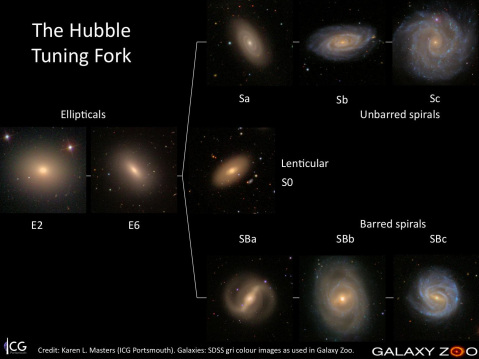
\includegraphics[width=4.5in]{Figures/Masters_tuningfork.jpg}
\caption[Hubble tuning fork]{i'm a caption}
\label{fig: tuning fork}
\end{figure}

The oldest and arguably simplest system for categorizing galaxy morphology dates back to the 1930s and Edwin Hubble's famous ``tuning fork''. Based on a small sample, Hubble classified galaxies into two major groups, elliptical and spiral. Visually, elliptical galaxies possessed a smooth light distribution while spirals are characterized by well-defined disk structure with spiral arms. Hubble assigned a number to elliptical galaxies denoting the degree of their ellipticity, where 0 corresponds to a nearly perfectly round galaxy and 7 being highly elongated. Spirals were given additional designation in the form of letters a through c, characterizing the compactness of their spiral arms. For example, ``Sa'' galaxies are tightly wound, whereas "Sc" spirals are looser. The spiral category was then further subdivided by galaxies that exhibited a central bar. There is also indications that the bulges inherent to many spiral galaxies share a close connection to elliptical galaxies. 

It became common to call galaxies on the left side of the diagram ``early-types,'' and those on the right ``late-types''. Contrary to this author's belief, Hubble never intended these designations to imply galactic evolution. Instead, this terminology was borrowed from stars, where massive O and B stars were referred to as ``early-type'', while older stars were known as ``late-type''\citep{Buta2011}. It has subsequently become clear that, much to the contrary, ellipticals are dominated by late-type stars while disk galaxies are typically composed of young, early-type stars.  Unfortunately, the misnomer has stuck. 

%This hybrid category, denoted S0 on the tuning-fork diagram, was originally thought to be a transition stage between these two fundamental galaxy types. Additionally, it was surmised that galaxies travelled along the Hubble tuning fork from left to right. While this theory has literally been turned on its head, astronomers are unfortunately left with the misnomer of ``early-'' and ``late''-type galaxies referring to ellipticals and spirals respectiively. 


This method of galaxy classification was based on an extremely small sample of which only a few percent did not conform to the basic designations originally posited by Hubble. These leftover galaxies were dubbed ``Irregulars'' or ``peculiars''. It wasn't until much later that it was discovered these types of galaxies are far more prevalant than Hubble originally thought. Since this early attempt at classification, several other systems have been put forward but most share the same basic categories. Indeed, even this simplistic approach has yielded nearly a hundred years of science that has advanced our understanding of galaxy formation, structure, and evolution. 
 


\section{Morphology as a tracer of galaxy evolution}
Though simple, these basic categories have proved to then segue into how those different morphologies provide detailed insights into formation and evolution. Give examples of the science that can be gleaned from broad classifications (early- vs late-type galaxies), and how rare classifications can provide unique viewpoints (clumpy galaxies at low redshift, or green peas, i.e.)

Any theory of galaxy formation and evolution will
have to, at some point, account for the bewildering array of galactic forms. --Buta
 Galaxy morphology is strongly correlated with galactic star formation history. Galaxies
where star formation ceased gigayears ago tend to look very different from those where star
formation continues at the present time. 


\subsection{Stellar populations and star-formation histories}
At its heart, morphology simply traces an integrated 2D projection of a galaxy's light distribution. As such, it encodes information on the distribution of a galaxy's stellar, gas, and dust content. However, these components are best traced through different wavelengths of light. 

Consider a coevolving stellar population with a mass distribution according to your favorite initial mass function. Stars on the Main Sequence (MS) radiate in the blue and ultraviolet (UV) end of the spectrum due to their high effective temperatures. The most massive quickly evolve off the MS and become red supergiants causing a decrease in the UV flux and an increase in the near infrared (NIR). As the low mass stars in this stellar population continue to evolve off the MS, the UV flux steadily decreases until eventually the red giant branch becomes the dominant source of flux, radiating in the IR. This so-called \textit{passive} evolution indicates that as a galaxy ages it becomes redder. A galaxy's morphology is tightly correlated with its color: massive elliptical galaxies are typically referred to as ``red and dead,'' possessing old stellar populations, while disk galaxies are generally still undergoing star formation and thus possess young, bluer stellar populations \citep[e.g.,][]{Strateva2001,Baldry2004b, Cirasuolo2007, Lee2013, Taylor2015}. This dichotomy is so prBevalent that color has been used as a proxy for morphology when acquiring the latter was impractical \citep[e.g.,][]{Shen2003, Blanton2003c}. 

Furthermore, this color bimodality correlates with luminosity resulting in the color-magnitude relation (CMR) \citep{Baldry2004a, Bell2004}. Now ubiquitous, this relation visualizes the separation of galaxy colors as a function of luminosity resulting in three main categories: the blue cloud, the red sequence and, more recently recognized, the green valley. Studies have shown that the red sequence is dominated by early-type galaxies like elliptical/S0 while disk galaxies reside in the blue cloud. There is a distinct gap between these two galaxy populations but recent studies have shown that, though sparse, galaxies also reside here. The top panel of Figure XXX \citep[credit:][]{Kormendy2012} shows an example of the color-magnitude relation for a sample of SDSS galaxies while the bottom panel depicts a schematic of the associated morphologies. 

\begin{figure}
\centering
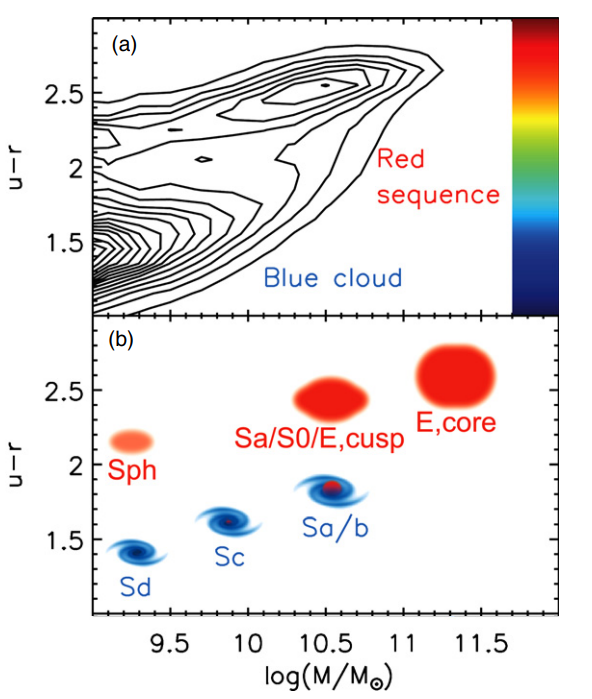
\includegraphics[width=3.5in]{Figures/kormendy_CMR.png}
\caption{Color-magnitude (mass) relation schematic \citep[credit:][]{Kormendy2012}.}
\end{figure}

For early-type galaxies, the color-magnitude relationship is more significant and provides a tool to constrain the star-formation histories of this galaxy population \citep{Sandage1978, Tully1982}. There exists a degeneracy between the age and metallicity of stellar populations: though older stars tend to be redder, this effect can also be achieved through an increase in stellar metallicity. It is now believed that the slope of the CMR is due primarily to metallitcy effects \citep{Bower1992, Kodama1997}, which then allows for age estimates to be placed on the last episode of significant star formation in early-type galaxies \citep[e.g.,][]{LopezCruz2004}. The small scatter in this relation reflects that these galaxies have old, passively evolving stellar populations. 

put this somewhere \citep{Mei2009}
%Galaxies contain more than just stars; gas and dust can also alter a galaxy's morphology. Dust is thought to be produced in AGB stars and distributed to the interstellar medium via stellar winds. Disk galaxies typically have more dust than ellipticals indicating that early-type galaxies expelled their dust content via dramatic mergers \citep{some people}. Blue light is more strongly attenuated than red light. This causes the dust to heat and radiate in the IR making a galaxy appear redder than it would otherwise. Another, more dramatic example of dust's effect on a galaxy's morphology is the dust lanes exhibited by many spiral galaxies. 

%It is clear that to fully understand a galaxy's composition, studying the morphology through observations across the electromagnitic spectrum is necessary: cold dust indicative of recent galaxy-galaxy interaction can be determine through radio observations of HI gas; infrared observations shed light on the dust content and old stellar components, visual and UV observations trace ever stellar nurseries, and high energy observations like X-rays give a tantalizing peak at what lurks in the bulges of active galaxies. 


\subsection{Mass and luminosity functions and galactic growth}
The most fundamental characteristic of a galaxy is its mass, however, this is a difficult quantity to measure. Much easier, instead, is a measurement of a galaxy's luminosity which takes only an image to estimate. Because the luminosity is, in large part, an integration of stellar light, mass generally scales with luminosity. The correlation of morphology with luminosity thus also implies a dependence on galaxy mass. A cottage industry for decades, constructing mass and luminosity functions has provided insights into the build-up of baryonic mass over cosmic time. 
In priniciple, the star formation density at a given epoch should represent the integral of the SF density up to that redshift. 

Stellar mass functions (SMFs) are a key first-order observatble that allows one to statistically trace back the formation of stars in the universe. Comparison with predicted SMFs further constrains the mechanisms with which galaxies converst 

Nearly half of the stellar mass in the local universe resides in early-type galaxies with half in late-type disk structures \citep{Kelvin2014}. However, this was not always the case.  Prior to z of 2, Hubble type morphologies become vague and are dominated by pecular galaxies \citep{Dickenson2000,Papovich2005,Cameron2011,Conselice2005,Conselice2011,Buitrago2013}and thus considerable evolution has taken place since that epoch. It has been shown that the Hubble morphologies emerge between 1 < z < 3 indicating that the peculiar high-redshift systems settle down into the galaxies we see in the local universe \citep{Mortlock2013}. 

It has been postulated that these early galaxies' evolution is dominated by violent mergers into spheroidal systems\citep{Driver2013,Bluck2009,Man2012}. After redshift 2 the dominant mechanism for galaxy evolution switches to cold gas accretion and hence the formation of of disk galaxies \citep{Conselice2013}. Of course, these processes are also presumed to be mass-dependent with the most massive galaxies settling into the familar Hubble sequence more quickly than low-mass galaxies \citep{Buitrago2013,Conselice2011,Mortlock2013}

Understanding the rate of growth and distribution of baryonic mass in galaxies provides constraints on the mechanisms necessary to produce such observations. It is well known that there was a period of increased star formation at z>2 when many galaxies rapidly formed stars at rates not typically observed in the local universe. However this formation was not distributed equally among all galaxies and types and the subsequent evolution of the star formation density of the universe paints a picture in which.. blah blah blah. 

A z$\sim$2, most of the stellar mass density is in irregular galaxies \citep{HuertasCompany2016} but this drops with redshift until, in the local universe, irregulars only dominate the SF density in low-mass galaxies. The abundance of passive (early-type) galaxies steadily increases from z 4 up until the present epoch. 

The quenching of star formation produces the color bimodality of galaxies, is likely the cause of the decrease in the star-formation rate density in the universe since z of 2 and could also be associated with morphological transformations within galaxies. 

The shape of the SMFs of galaxies has a knee corresponding to a characteristic stellar mass around 10^10.7 which appears to be independent of redshift. This implies that galaies tend to cease forming stars at this characteristic mass. This takes place primarily at z > 1 because, at later times, there are more passive, early-type galaxies than late-type star-forming galaxies with this particular mass. 


Mass build up over cosmic time: galaxies grow differently based on their morphology. Bivariate mass-luminosity function. Shen2003. Ellipticals gain X amount of mass since z~1 but only gain how much in size? On the other hand, disks are entirely different... suggests different growth mechanisms demarcated by optical morphology. 

stellar mass functions for disks and spheriods \citep{Thanjavur2016,Bell2003}
mass assembly history \citep{Bundy2005, Taylor2015, Brinchmann2000}
luminosity and mass functions \citep{Blanton2003b, Blanton2001}


In heirarchical models, morphologies transform according to the mass characteristics of mergers. We find no evidence for any change in the mass density of
spiral galaxies, suggesting the merging of spiral galaxies into
elliptical galaxies between and the present cannot be a z = 1
dominant process. Moreover, the total stellar mass density
hardly increases over the range sampled. Both results support
the contention that most massive galaxies formed their stars
prior to or around . Lower mass galaxies remain active z = 1
to much more recent epochs, consistent with the “downsizing”
picture introduced by Cowie and collaborators. --Brinchmann and Ellis


\subsection{Morphology as a function of environment}
A galaxy's environment also has a direct relationship with its morphology. First quantified by \cite{Dressler1980}, the morphology-density relation is an emperical observation that elliptical galaxies tend to reside in the densest environments, i.e., rich groups and clusters, at all stages of cosmic time. in the richest and densest clusters of galaxies, the dominant morphology is elliptical, while for field galaxies, the dominant morphology is spiral. Furthermore, it's been determined that this relation evolves over time, at least for the densest environments. All of this points to scenarios in which the environment of a galaxy dictates, or influences its morphology and that the processes contributing to this effect have evolved with time. \citep[e.g.,][]{Fasano2000, Shen2003, Smith2005, Peng2010}

Much study has been done to separate the effects of environment from mass, i.e., secular, causes of morphological features. Peng, Shen,,etc. Cluster environments are, compared to the field, extremely hot and dense. Galaxies residing in these environments have faster velocity, on average. (What kind of v is that called again? I forgot.)  It's estimated that field galaxies are, on average, 1 per Mpc (?). The merging rate depends on the density of galaxies. In the past galaxies were closer together so merging was a bigger deal. Logically then, it would seem that merging happens all the timein clusters and that this then causes a morphological change from disk to elliptical. However, galaxies are moving so briskly in clusters that it becomes less likely that they collide! Instead, merging seems to be a predominant morphological mechanism in groups rather than clusters. In clusters, instead, other physical processes shape the way a galaxy evolves and looks over time. 

Spirals convert to S0/elliptical galaxies in clusters due to several processes: they should have lost their cold atomic and molecular gas via ram pressure stripping (but see Tonnesen \& Bryan 2009, for the effect of ram
pressure on molecular clouds), harassment (Moore et al. 1996),
strangulation (Kawata \& Mulchaey 2008), etc.


role of mergers CANDELS \citep{Karteltepe2010}
mergers and AGN \citep{Kocevski2012, Villforth2014}

\subsection{Insights from rare morophologies}
So far I've examined insights gleaned by considering large populations of galaxies split into broad categories of early- and late-types. Though unbeknownst to Hubble, it is now well known that galaxy structure and hence the integrated light profile is much more complicated and varied. Examing both finer galactic structure such as bars, as well as rare morphologies like the ``green peas'' has pushed the boundaries on our collective knowledge of galaxy evolution. What have we learned from the green peas? Clumpy galaxies at low redshift? Ring galaxies? 

-- insights concerning dynamical disks; star formation; blah. 


\section{Obtaining morphological designations}
Now that we all believe we should get these morphologies -- how should we do it? 

\subsection{Visual classifications}
The history of galaxy morphology assignment is rife with historical precendents due in large part to Edwin Hubble's original ``tuning fork.'' Seeing as Hubble originally thought these `nebulae' were features residing in our own galaxy, we end up with goofy shit where we call elliptcals ``early-type'' and disks ``late-type'' though subsequent studies all confirm that the ages of ellipticals are far older than those of spiral galaxies. 

Visual classification, though highly accurate due to the human mind's unique pattern recognition capability, is, however, entirely slow. Assignment of morphological type to galaxies thus resulted in small samples lacking statistical signifigance for decades (until the use of cartels of graduate students wherein morphologies for galaxy samples reached a few thousands). With surveys such as the Sloan Digital Sky Survey looming on the horizon, a new approach would be necessary in order to take advantage of the unique insights provided by galaxy morphologies.

This necessitated the birth of the Galaxy Zoo project, the first effort to crowd-source the task of galaxy morphology assignment to the general public. Blah blah blah Galaxy Zoo blah. 

While the Galaxy Zoo project has provided a solution that scales visual classification for current surveys  by harnessing the combined power of thousands of volunteers \citep{Lintott2008, Lintott2011, Willett2013, Willett2017, Simmons2017},  producing a prolific amount of scientific output \citep[e.g.,][]{Land2008, Bamford2009, Darg2010, Schawinski2014, Galloway2015, Smethurst2016}; upcoming surveys such as \textit{LSST} and \textit{Euclid} will require a different approach, imaging more than a billion new galaxies  \citep{LSST, Euclid}.  If detailed morphologies can be extracted for just  0.1\% of this imaging, we will have millions of images to contend with. A project of this magnitude would take more than sixty years to classify at Galaxy Zoo's current rate and configuration. Standard visual morphology 
methods will thus be unable to cope with the scale of data. 


Visual classification by experts: CANDELS \citep{Kartaltepe2015}

\subsection{Automated classifications}
Another approach has been the automated extraction of galaxy morpholgies with the development of both parametric and non-parametric structural indicators. 

It is well known that a galaxy's light profile can be modelled according to the function [insert function here] where the Sersic index, $n$, has been shown to correlate strongly with a distinction between early- and late-type galaxies. In particular, a Sersic index of $n=4$ corresponds to a de Vaucouleurs' profile which well describes the surface brightness of an elliptical galaxy as a function of its apparent radius from the galaxy's center. On the other hand, a Sersic index of $n=1$ describes an exponential profile which is a good description for spiral galaxies. 

A drawback to the parametric approach is the need to assume the underlying distribution and while this works technique works well for galaxies that are obviously elliptical or spiral, it produces mixed results for other morphological types, i.e., irregulars or peculiars, which have low central concentration resulting in a low Sersic index, but which do not have disks or spiral arms. 

Non-paramteric structural indicators require fewer assumptions on the data and are instead derived observationally. Several of these diagnostics have been developed over the past couple decades, each probing a different part of the galaxy's light profile and thus its overall dynamical distribution. The most common diagnostics are described below. 

Closely related to the Sersic index is the non-paramatric diagnostic of concentration. A galaxy's concentration aims to identify how dense a galaxy's central surface brightness profile is. Concentration, originally conceived by Abraham(?) has had several definitions over the years. The most common consider the ratio of the aggregated light within two concentric apertures about the galaxy's center. Typically, these apertures contain 50 and 90\% of the galaxy's light (another common approach is to use 50\% and 80\%). Because 


Example of using parametric Sersic profile to classify galaxies as early-/late-type:
``We show that the wavelength-dependence of n may be employed to separate visually-classified early- and late-type galaxies in a manner similar to the use of colour and n. Furthermore, we find that the wavelength variation of n can recover galaxies that are misclassified by these other morphological proxies."\citep{Vika2015}

Peng(?) [was that the first?] developed the first model to decompose a galaxy's light profile into 

The radial luminosity profile of a disk is usually exponential, with departures from an
exponential being due to the presence of other structures. --Buta

Another approach has been the automated extraction of morphologies with the development of parametric \citep{Sersic1968, Odewahn2002, Peng2002}, and non-parametric 
\citep{Abraham1994, 
	   Conselice2003, 
	   Abraham2003, 
	   Lotz2004,  
	   Freeman2013} 
structural indicators. While these scale well to large samples 
\citep[e.g.,][]{Simard2011, 
			Griffith2012, 
			Casteels2014, 
			Holwerda2014, 
			Meert2016}, 
they often fail to capture detailed structure and can provide only statistical morphologies with large uncertainties \cite[e.g.,][]{Abraham1996, Bershady2000}. 


\subsection{Machine learning}
Machine learning techniques are becoming increasingly popular for classification and image processing tasks. Another automated approach, these generally work by defining a set of features that describe the morphology in an $N$-dimensional space. The location in this morphology space defines a morphological type for each galaxy. Learning the morphology space can be achieved through algorithms such as Support Vector Machines \citep{HuertasCompany2008} or Principal Component Analysis \citep{Watanabe1985, Scarlata2007}. Another approach is through deep learning, a machine learning technique that attempts to model high level abstractions. Algorithms like convolutional and artificial neural networks (CNNs, ANNs) have been used for galaxy morphology classification with impressive accuracy 
\citep{Ball2004, 
	Banerji2010, 
	Dieleman2015, 
	HuertasCompany2015}. 
A drawback to all machine learning classification techniques is the need for standardized training data, with more complex algorithms requiring more data. Furthermore, these data must be consistent for each survey: differences in resolution and depth can be implicitly learned by the algorithm making their application to disparate surveys challenging. 


\section{Overview of Galaxy Zoo: Express}

 In this work we present a system that preserves the best features of both visual and automatic classifications, developing for the first time a framework that brings both human and machine intelligence to the task of galaxy morphology to handle the scale and scope of next generation data. We demonstrate the effectiveness of such a system through a re-analysis of visual galaxy morphology classifications collected during the Galaxy Zoo 2 project, and combine these with a Random Forest machine learning algorithm that trains on a suite of non-parametric morphology indicators widely used for automated morphologies. In this paper we focus on the first question of the Galaxy Zoo decision tree. We demonstrate that our method provides a factor of 11.4 increase in the rate of galaxy morphology classification  while maintaining at least 93.5\% classification accuracy as compared to Galaxy Zoo 2 published data. We first present an overview of our framework, which also serves as a blueprint for this paper. 


%%%-------------------------------------------------------
%%% FIGURE:     GZ EXPRESS Schematic
%%%-------------------------------------------------------
\begin{figure*}[ht!]
%\figurenum{1}
\plotone{Figures/human_machine/f1.pdf}
\caption[Schematic of the Galaxy Zoo: Express human+machine hybrid system.]{Schematic of our hybrid system. Humans provide classifications of galaxy images via a web interface. We simulate this with the Galaxy Zoo 2 classification data described in Chapter~\ref{chap:2}. Human classifications are processed with an algorithm described in Chapter~\ref{chap:3}. Subjects that pass a set of thresholds are considered human-retired (fully classified) and provide the training sample for the machine classifier as described in Chapter \ref{chap:4}. The trained machine is applied to all subjects not yet retired. Those that pass an analogous set of machine-specific thresholds are considered machine-retired. The rest remain in the system to be classified by either human or machine. This procedure is repeated  nightly. \label{fig: schematic}}
\end{figure*}


%%----------------------------------------------------------------------------------------------------------------------------------------------------
%%   GALAXY ZOO EXPRESS OVERVIEW
%%---------------------------------------------------------------------------------------------------------------------------------------------------

The Galaxy Zoo Express (GZX) framework combines human and machine to increase morphological classification efficiency, both in terms of the classification rate and required human effort. Figure~\ref{fig: schematic} presents a schematic of GZX including section numbers as a shortcut for the reader. We note that transparent portions  of the schematic represent areas of future work which we explore in Chapter \ref{chap:summary}. Any system combining human and machine classifications will have a set of generic features: a group of human classifiers, at least one machine classifier, and a decision engine which determines how these classifications should be combined.

In this work we demonstrate our system through a re-analysis of  Galaxy Zoo 2 (GZ2) classifications. This allows us to  create simulations of human classifiers. These classifications are used most effectively when processed with SWAP, a Bayesian code described in Chapter \ref{chap:3}, first developed for the Space Warps gravitational lens discovery project~\citep{Marshall2016}. These subjects provide the machine's training sample. 

In Chapter~\ref{chap:4}, we incorporate a machine classifier. We have developed a Random Forest algorithm that trains on measured morphology indicators such as Concentration, Asymmetry, Gini coefficient and \M{20} well-suited for the top-level question of the GZ2 decision tree, discussed in Chapter \ref{chap:2}. After a sufficient number of subjects have been classified by humans, the machine is trained and its performance assessed through cross-validation. This procedure is repeated nightly and the machine's performance increases with size of the training sample, albeit with a performance limit. Once the machine reaches an acceptable level of performance it is applied to the remaining galaxy sample. 

Even with this simple description, one can see that the classification process will progress in three phases.  First, the machine will not yet have reached an acceptable level of performance; only humans contribute to subject classification. Second, the machine's performance will improve; both humans and machine will be responsible for classification. Finally, machine performance will slow; remaining images will likely need to be classified by humans. This blueprint allows even modest machine learning routines to make significant contributions alongside human classifiers and removes the need for ever-increasing performance in machine classification.

% The main Chapters 
%!TEX root = thesis.tex

\chapter{Data: visual and automated morpholgies}
\label{chap:2}


This chapter presents all data used in this research. It begins with an in depth overview of the Galaxy Zoo 2 project, including the galaxy sample and procurement of visual galaxy morphology classifications. It then covers in considerable detail the methodology for obtaining the morphological structural indicators measured for the Galaxy Zoo 2 sample. 


%%%%%%%%%%%%%%%%%%%%%%%%%%%%%%%%%%%%%%%%%%%%%%%%%%%%%%%%%%%%%%%%%%%%%%%%%%
%%%		SECTION: 	GALAXY SAMPLE SELECTION
%%%%%%%%%%%%%%%%%%%%%%%%%%%%%%%%%%%%%%%%%%%%%%%%%%%%%%%%%%%%%%%%%%%%%%%%%%
\section{Galaxy Zoo}
Founded by co-creators Chris Lintott and Kevin Schawinksi, Galaxy Zoo is a crowd-sourced innitiative to visually classify large numbers of galaxies by enlisting members of the general public. The original project \citep[GZ1,][]{Lintott2008} began in 2007 with the classification of 893,212 galaxy images from the Sloan Digital Sky Survey (SDSS) Data Release 6 with $r < 17.77$ Petrosian AB magnitudes \citep{Strauss2002,Adelman2008}. The first iteration of the project was simplistic, inviting volunteers to determine whether a galaxy was elliptical, spiral, or a star / artifact. The project was an immediate success both in terms of the public interest and the resulting science: following its completion \citep{Lintott2008}, over a dozen peer-reviewed articles utilzing GZ1 classifications\footnote{\url{https://www.zooniverse.org/about/publications}} were published. In addition to explorations of galaxy morphology and its dependence on color and environment \citep{Skibba2009, Bamford2009}, significant results also included the discovery of substantial populations of red disks \citep{Masters2010b} and blue ellipticals \citep{Schawinski2009}, as well as discoveries of rare objects such as the ``green peas'' \citep{Cardamone2009} and Hanny's Voorwerp \citep{Lintott2009}, the first obvservation of an AGN ionization echo. 

The early sucess of GZ1 led to several subsequent and progressively more complex projects. To date, Galaxy Zoo has provided morphologies for over a million galaxies from multiple imaging surveys of various wavebands and redshifts using classifications provided from over a hundred thousand volunteers. The research presented in this thesis utilizes data from the Galaxy Zoo 2 project \citep[GZ2,][]{Willett2013}, the immediate successor of GZ1. The following sections provide an overview of the GZ2 project including the galaxy sample, the decision tree structure, and a brief description of how volunteer votes are converted into descriptive classifications. 
%A summary of Galaxy Zoo projects is given in Table XXX. 

%%%%%%%%%%%%%%%%%%%%%%%%%%%%%%%%%%%%%%%%%%%%%%%%%%%%%%%%%%%%%%%%%%%%%%%%%%
%%%		SUBSECTION:		GALAXY SAMPLE SELECTION
%%%%%%%%%%%%%%%%%%%%%%%%%%%%%%%%%%%%%%%%%%%%%%%%%%%%%%%%%%%%%%%%%%%%%%%%%%
\subsection{Galaxy sample selection}
The original GZ1 project sought classifications for nearly one million galaxies in SDSS. Due to the staggering galaxy sample size, the morphologies collected were broad, seeking to determine between early-type, late-type and mergers. However, much can be gained by probing detailed morpholgies such as the existance of bars, bulges, dust lanes, rings, etc. Galaxy Zoo 2 thus selected the nearest and brightest 25\% of galaxies from the original GZ1 sample, galaxies for which fine morphological structure could be resolved and classified. Pulled from the Data Release 7 Legacy catalog \citep{Abazajian2009} which imaged the the North Galactic Cap, this galaxy sample required the Petrosian half-light magnitude be brighter than 17.0 in the $r$-band, along with a size limit such that \texttt{petror90\_r} $>3\arcsec$, where \texttt{petror90\_r} is the radius containing 90\% of the $r$-band Petrosian aperture flux. Spectroscopic redshifts were pulled from the SDSS Main Galaxy Sample \citep{Strauss2002} and galaxies outside of $0.0005 < z < 0.25$ were removed, though objects without reported redshifts remained in the sample. This resulted in a sample of 273,783 galaxies. 

In addition to the DR7 Legacy catalog, galaxies were included from Stripe 82, a multiply-imaged strip along the celestial equator in the Southern Galactic Cap. Galaxies in this region were selected to have $m_r\le17.7$. GZ2 included multiple samples from this region: a set of 21,522 single-exposure images (though only about half conformed to the shallower Legacy magnitude cut specified above), and two sets of $\sim$30K co-added images from multiple exposures resulting in an object detection limit approximately two magnitudes deeper than the normal depth imaging. The research presented in this thesis utilizes the final GZ2 single-depth sample consisting of 295,305 galaxies of which 11,334 have the deeper magnitude limit. 


%%%%%%%%%%%%%%%%%%%%%%%%%%%%%%%%%%%%%%%%%%%%%%%%%%%%%%%%%%%%%%%%%%%%%%%%%%
%%%		SUBSECTION:		GZ2 DECISION TREE / PROJECT HISTORY
%%%%%%%%%%%%%%%%%%%%%%%%%%%%%%%%%%%%%%%%%%%%%%%%%%%%%%%%%%%%%%%%%%%%%%%%%%
\subsection{GZ2 decision tree and project history}
GZ2 was the first Galaxy Zoo project to utilize a decision tree wherein, with the exception of the first question, subsequent tasks depended on the response to the current question. The full decision tree is shown in Figure \ref{fig: gz2 decision tree}. Volunteers are allowed to select a single option for each question and are immediately taken to the next task after responding.  Using GZ2 nomenclature, a \textit{classification} is the total amount of information about a subject obtained by completing all tasks in the decision tree. Each step in the tree is a \textit{task} consisting of a \textit{question} and a set of \textit{responses}. A volunteer's response is referred to as a \textit{vote}. The first question in the tree is a modification of the GZ1 project, asking volunteers to identify whether a galaxy is `smooth', has `features or a disk', or is a `star or artifact'. 

%%%%%%%%%%%%%%%%%%%%%%%%%%%%%%%%%%%%%%%%%%%%%%%%%%%%%%%%%%%%%%%%%%%%%%%%%%
%%%		FIGURE: 	GZ2 DECISION TREE
%%%%%%%%%%%%%%%%%%%%%%%%%%%%%%%%%%%%%%%%%%%%%%%%%%%%%%%%%%%%%%%%%%%%%%%%%%
\begin{figure}[h!]
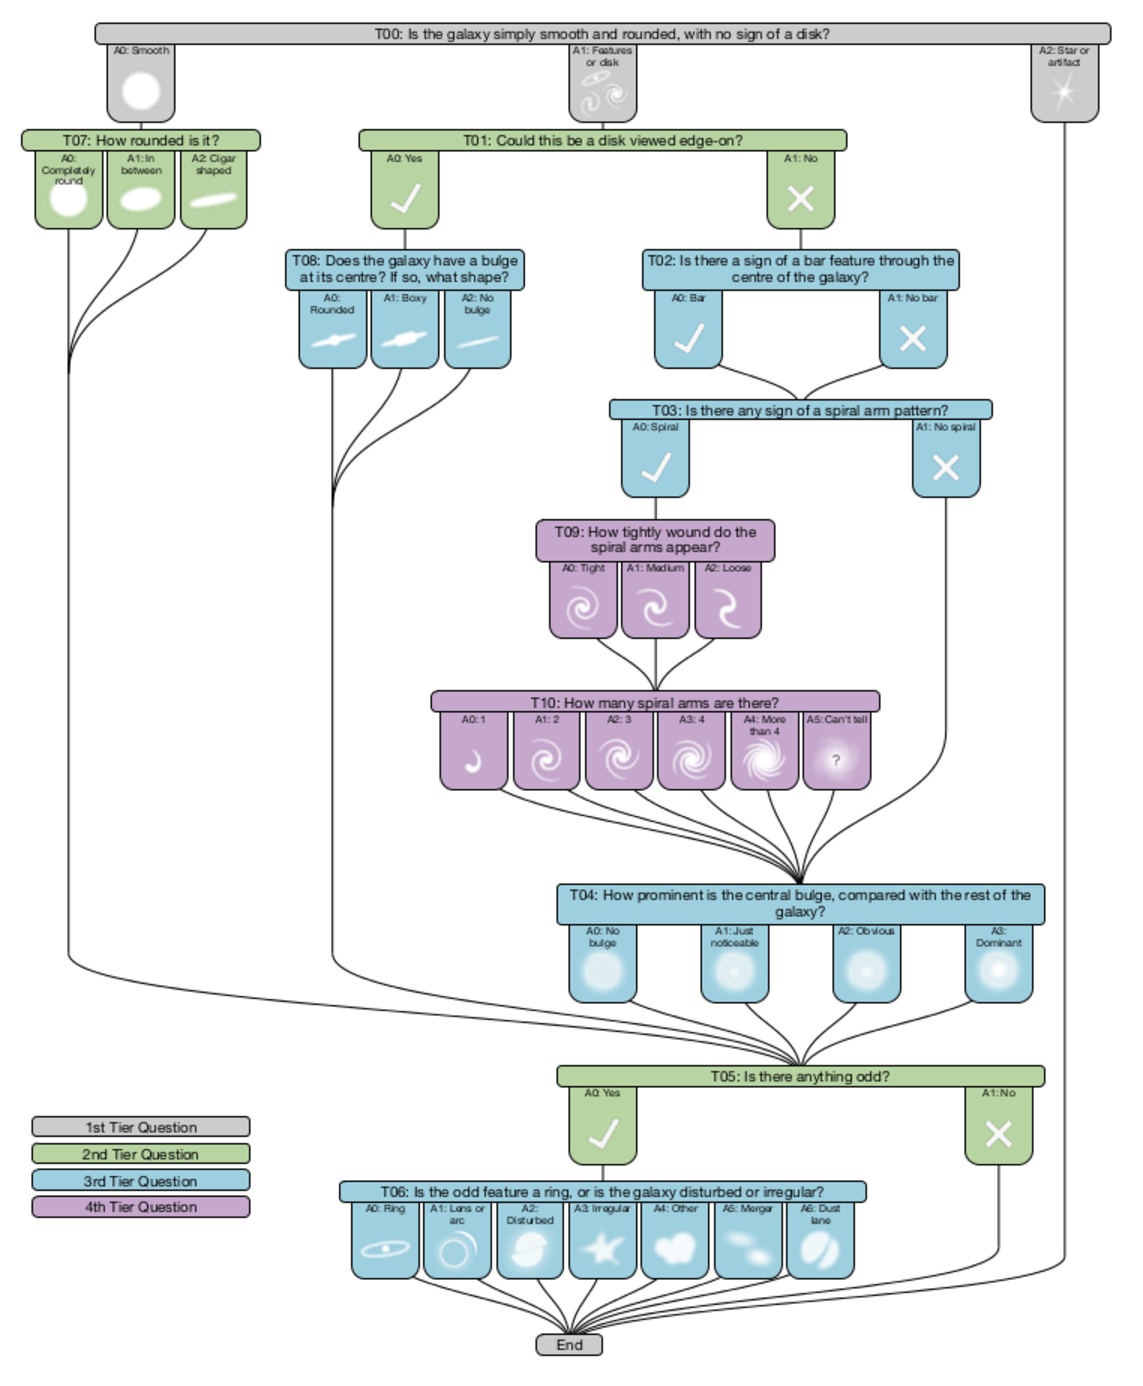
\includegraphics[width=\textwidth]{Figures/gz2_tree.pdf}
\caption[Galaxy Zoo 2 decision tree]{Galaxy Zoo 2 decision tree structure.}
\label{fig: gz2 decision tree}
\end{figure}

For the single-depth sample, volunteers were shown color images generated from the SDSS ImgCutout web service. Each image is a $gri$ color composite scaled to $0.02\times$\texttt{petror90\_r}. Throughout the life of GZ2 these images were randomly served to a web interface similar to that shown in Figure \ref{fig: gz2 interface}. Towards the end of the project galaxy images with few responses were shown more frequently in order to ensure that each galaxy had a sufficient number of classifications to adequately characterize the classification distribution. This resulted in a median of 44 classifications per galaxy with a wide spread. The full project spanned just over 14 months with the final dataset consisting of over 16 million classifications from over 80 thousand volunteers. 
 
%%%%%%%%%%%%%%%%%%%%%%%%%%%%%%%%%%%%%%%%%%%%%%%%%%%%%%%%%%%%%%%%%%%%%%%%%%
%%%		FIGURE: 	GZ2 WEB INTERFACE
%%%%%%%%%%%%%%%%%%%%%%%%%%%%%%%%%%%%%%%%%%%%%%%%%%%%%%%%%%%%%%%%%%%%%%%%%%
\begin{figure}[h!]
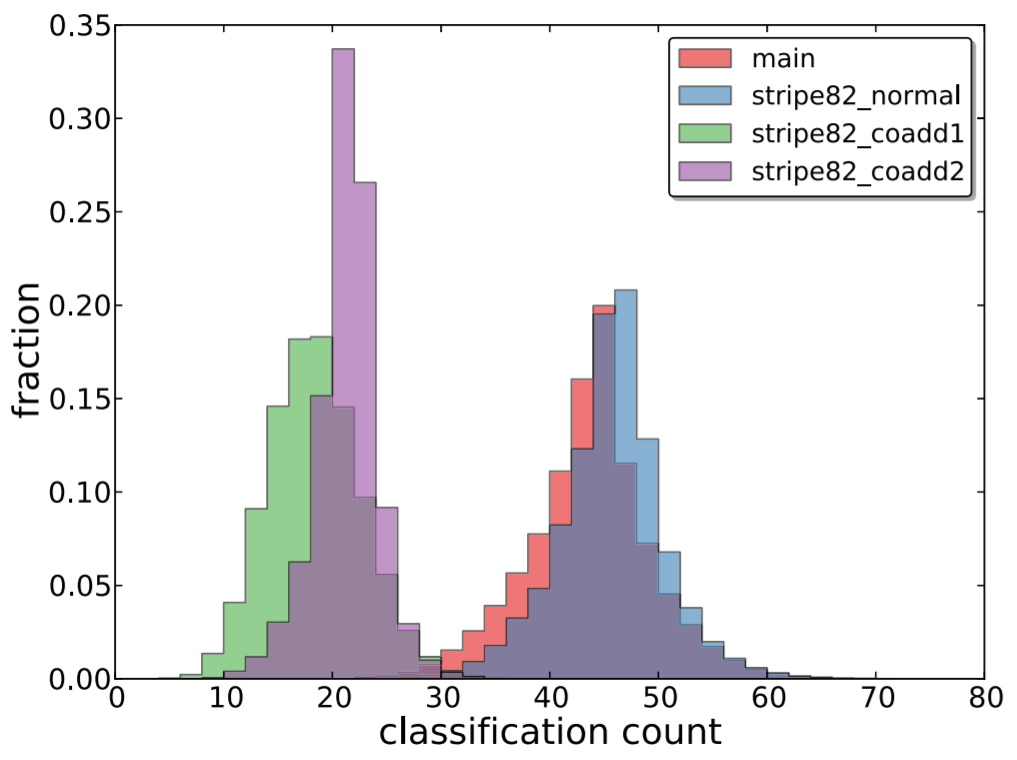
\includegraphics[width=\textwidth]{Figures/GZ2_classification_count.png}
\caption[Galaxy Zoo 2 classification count distributions]{Distribution of the classification counts for the various subsets of the GZ2 galaxy sample \citep[credit:][]{Willett2013}. In this thesis we use the main sample with a median of 44 votes per galaxy.}
\label{fig: gz2 interface}
\end{figure}

%%%%%%%%%%%%%%%%%%%%%%%%%%%%%%%%%%%%%%%%%%%%%%%%%%%%%%%%%%%%%%%%%%%%%%%%%%
%%%		SUBSECTION: 	DATA REDUCTION
%%%%%%%%%%%%%%%%%%%%%%%%%%%%%%%%%%%%%%%%%%%%%%%%%%%%%%%%%%%%%%%%%%%%%%%%%%
\subsection{Data reduction}
The GZ2 catalog provides several types of morphologies computed from volunteer classifications constisting of a vote fraction for each response to every task, denoted $f_{\mathrm{response}}$. The most basic of these is computed simply as $f_r = n_r/n_t$, where $n_r$ is the number of votes of response $r$, and $n_t$ is the total number of votes for task $t$. In future chapters, this type of vote fraction is referred to as the \textit{raw} vote fraction as no post-processing has been performed. 

All GZ projects perform a weighting scheme that evaluates the consistency of individual volunteers by assessing how their votes deviate from the majority for each task in the decision tree. This process effectively downweights volunteers whose responses are consistent with a random classifier. A volunteer's consistency, $\kappa$, for a given task is defined as 

\begin{equation}
\kappa = \frac{1}{N_r}\sum_{i=1}^{N_r}{\kappa_i}
\end{equation}
where $N_r$ is the total number of responses to a task, and $\kappa_i$ is $f_r$ if the volunteer's vote corresponds to response $i$, otherwise $\kappa=(1-f_r)$. Each volunteer is then assigned a mean consistency, $\bar\kappa$, which is the average consistency over all tasks. A weighting function is then applied according to  

\begin{equation}
w = \min({1.0, (\bar\kappa/0.6)^{8.5}}).
\end{equation}

All vote fractions are then recomputed using the volunteer weights and the process is repeated three times to assure convergence. The resulting vote fractions are dubbed \textit{weighted}. For GZ2, $w=1$ for $\sim$95\% of volunteers and thus the majority are treated equally. It's important to note that there is no up-weighting of exceptionally consistent volunteers.


Finally, vote fractions are adjusted for classification bias: a change in the observed morphology as a function of redshift that is independent of any true galaxy evolution. The galaxies in the GZ2 sample have $0.005<z<0.25$, a range that is shallow enough to justify an assumption of no significant evolution.  Thus, the presumed culprit is that more distant galaxies are, on average, smaller and dimmer making fine features more difficult to identify. This effect is not unique to visual classifications and can also affect automated morphologies. GZ2 corrects for this effect, briefly described below, producing \textit{debiased} vote fractions.

The general approach is such that, for a galaxy of a given size and brightness, a sample of other galaxies with similar characteristics will statistically share the same mix of morphologies. The GZ2 main galaxy sample is binned by Petrosian absolute magnitude (M$_r$) and the Petrosian half-light radius, R$_{50}$,  as well as by redshift. A baseline morphology ratio for each task in the tree is computed in the lowest redshift bin for those galaxies with confirmed spectroscopic redshifts and with a sufficient number of votes to yield statistically reliable classifications, i.e., at least ten votes for a given task. This baseline is then used to correct more distant redshift bins. A more detailed account can be found in \cite{Willett2013}.

%This thesis draws on the \textit{raw} vote fractions for reasons explained in Chapter \ref{chap:3}. Focus now turns to the methodology of measuring automatic morphological indictors which are used in Chapter \ref{chap:4} to train a machine classifier. 

%%%%%%%%%%%%%%%%%%%%%%%%%%%%%%%%%%%%%%%%%%%%%%%%%%%%%%%%%%%%%%%%%%%%%%%%%%
%%%		SECTION: 	AUTOMATIC MORPHOLOGY INDICATORS
%%%%%%%%%%%%%%%%%%%%%%%%%%%%%%%%%%%%%%%%%%%%%%%%%%%%%%%%%%%%%%%%%%%%%%%%%%
\section{Automatic morphology indicators}
This thesis seeks to draw on the best qualities of all galaxy morphology classification methods including using automated morphologies and machine learning algorithms, which provide speed and brute force. Any machine classifier must have a set of features from which to learn to differentiate between classes. These features can be anything that correlates or distinguishes among classes. In the case of galaxy morphology possible features could include pixel values, spectral indices, magnitude, color, etc. Choosing which features are most appropriate for a given task is a difficult undertaking as the field of machine learning provides little in the way of clear cut rules for feature selection. Too few features and a machine learning algorithm will be unable to learn the parameter space; too many features can result in the Curse of Dimensionality: as the dimensionality of the parameter space increases linearly, the number of samples required to learn that space increases exponetially! 

In this work we draw on the Zurich Estimator of Structural Types \citep[ZEST,][]{Scarlata2007}. ZEST utilized five features measured from the light profile of galaxies combined with a PCA analaysis to determine morphologies for 120K COSMOS galaxies. These features are well known to correlate strongly with the distinction between early- and late-type galaxies. In this section we discuss how these values are measured for the GZ2 SDSS galaxy sample. 

\subsection{Imaging data}
The Galaxy Zoo 2 main galaxy sample contained 295,305 galaxies though 11,334 are single-epoch imaging from the Stripe 82 region with m$_r > 17.0$, fainter than the rest of the galaxy sample. These galaxies are excluded from the main GZ2 classification catalog though classifications for these galaxies exist in Stripe 82-exclusive catalogs. However, because we utilize the raw volunteer classifications from the original GZ2 project, we include all single-epoch galaxy imaging in our current sample, regardless of magnitude limit.  

We obtain $i$-band imaging (with central wavelength 7480\AA) from SDSS Data Release 12 for 290,059 galaxies in the GZ2 project. Image identifiers such as \texttt{CAMCOL}, \texttt{RUN}, and \texttt{FIELD} are used to select over 151,987 SDSS fields. Because the original GZ2 project obtained imaging from DR7, we surmise that the route to some galaxies in DR12 have switched locations or identifiers thus explaining the loss of 5246 galaxies. Because this represents only 1.8\% of the total population, these galaxies were not tracked down at this time. Postage stamps of each galaxy are cut from these fields where the dimensions of each cutout are 4$\times$Petrosian radius as measured by the SDSS pipeline. Galaxies located within 4 Petrosian radii of the edge of a field were excluded as image mosaicing was not performed. This removed 7962 galaxies resulting in a final sample of 282,350 GZ2 galaxy postage stamps or 95.6\% of the original sample.

\begin{figure}
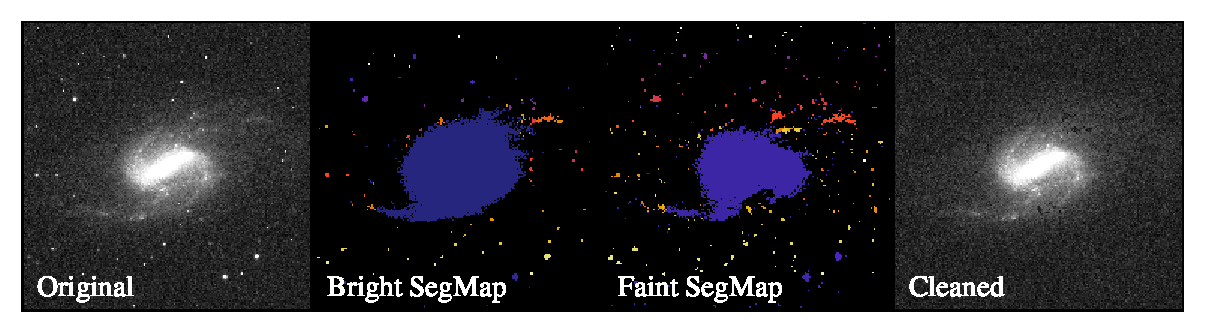
\includegraphics[width=\textwidth]{Figures/sextractor_example.pdf}
\caption[Example of Source Extractor segmentation maps.]{Example of SExtractor segmentation maps generated during the postage stamp cleaning process. The left panel shows the original $i$-band postage stamp, the middle two panels show the bright and faint segmentation maps where individual objects detected by SExtractor are shown on an arbitrary rainbow scale, and the right panel shows the resulting cleaned postage stamp.}
\label{fig: segmaps}
\end{figure}


\subsection{Image cleaning}
These postage stamps undergo a cleaning process in order to remove the light from nearby sources so as not to contaminate the light profile of the galaxy of interest. Each stamp is processed through Source Extractor \citep[ver. 2.8.6;][]{sextractor}, a software that automatically detects sources in CCD imaging based on a set of input parameters that control the object detection process. Two sets of parameters are used as it is unfeasible to find a single set of parameters that properly identifies all 282K galaxies. The first is designed to identify bright sources, while the second is better optimized to detect fainter objects. This software produces segmentation maps that identify the boundaries of each detected object in an image. By design, the galaxy of interest is located at the center of the cutout. Extraneous sources are then identifed from both the bright and faint segmentation maps and the pixels corresponding to these sources are replaced with a random value consistent with the background in that postage stamp.  An example of the segmentation maps created during this process is shown in Figure \ref{fig: segmaps}. Additionally, the first two columns in \Cref{fig: morph examples,fig: morph examples 2,fig: morph examples hardest} depict random samples of original and cleaned cutouts for a variety of ``difficulties,'' where the difficulty of successfully cleaning an image of all stray light from other nearby sources is dependent upon how many other sources exist in the postage stamp and how close those sources are to the galaxy of interest. 


\begin{figure}
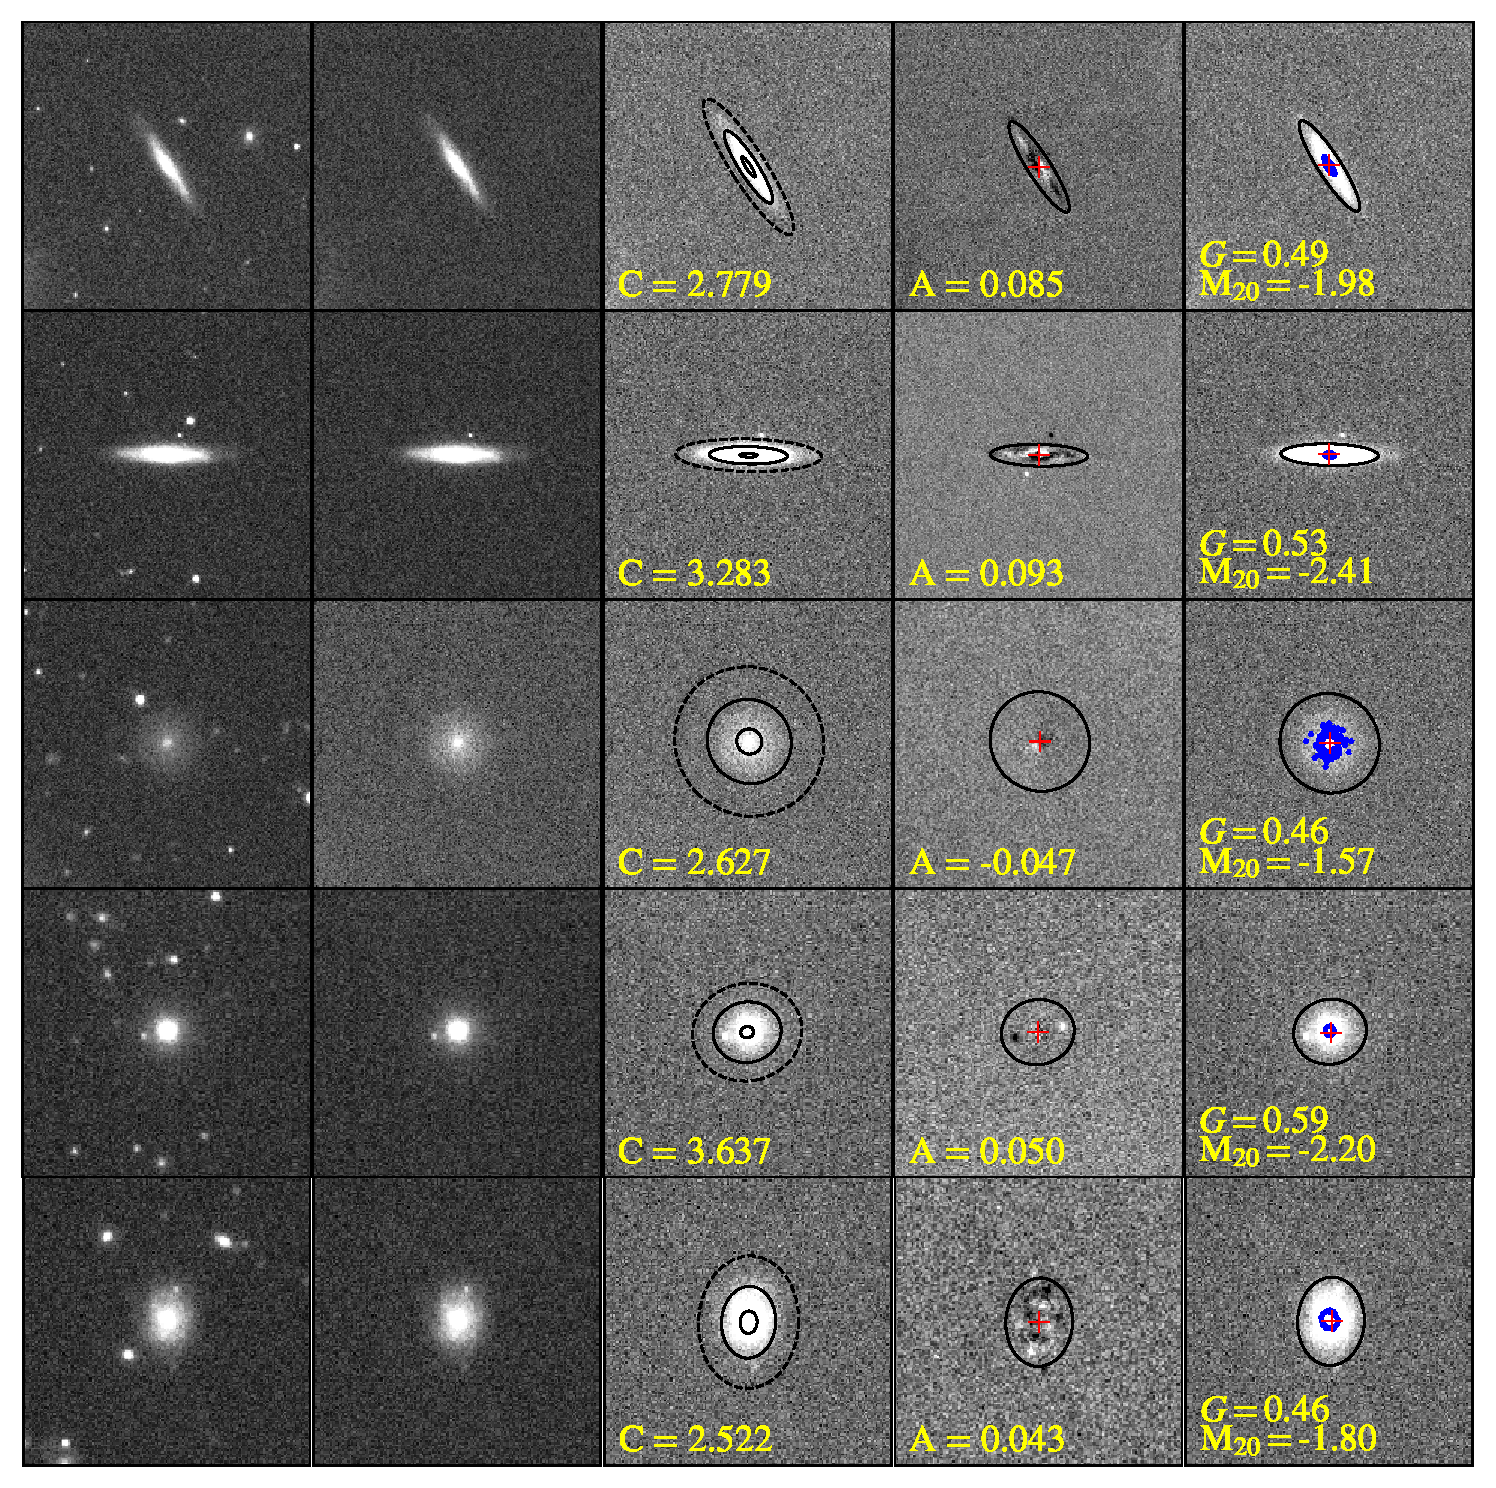
\includegraphics[width=\textwidth]{Figures/measure_morph_bin2_corrected.pdf}
\caption[Examples of image cleaning and morphology diagnostic measurements]{Examples of the postage stamp cleaning and morphology diagnostic measuring processes. The first and second columns show the original and cleaned $i$-band postage stamps. The third column shows the apertures used to calculate the concentration index where the two solid ellipses represent the apertures enclosing 20\% and 80\% of the galaxy total light which is defined as 1.5$\times$\rp~and shown as a dashed ellipse. The fourth column shows the residual asymmetry image generated according to Equation \ref{eqn: asymmetry} where the red cross denotes the galaxy's asymmetry center. The final column shows the Gini and \M{20} values where the red cross denotes the galaxy's \M{20} center and the blue contours trace the brightest 20\% of galaxy pixels. In the two rightmost columns, the solid ellipse represents 1\rp~within which all morphology diagnostics are computed.}
\label{fig: morph examples} 
\end{figure}


\begin{figure}
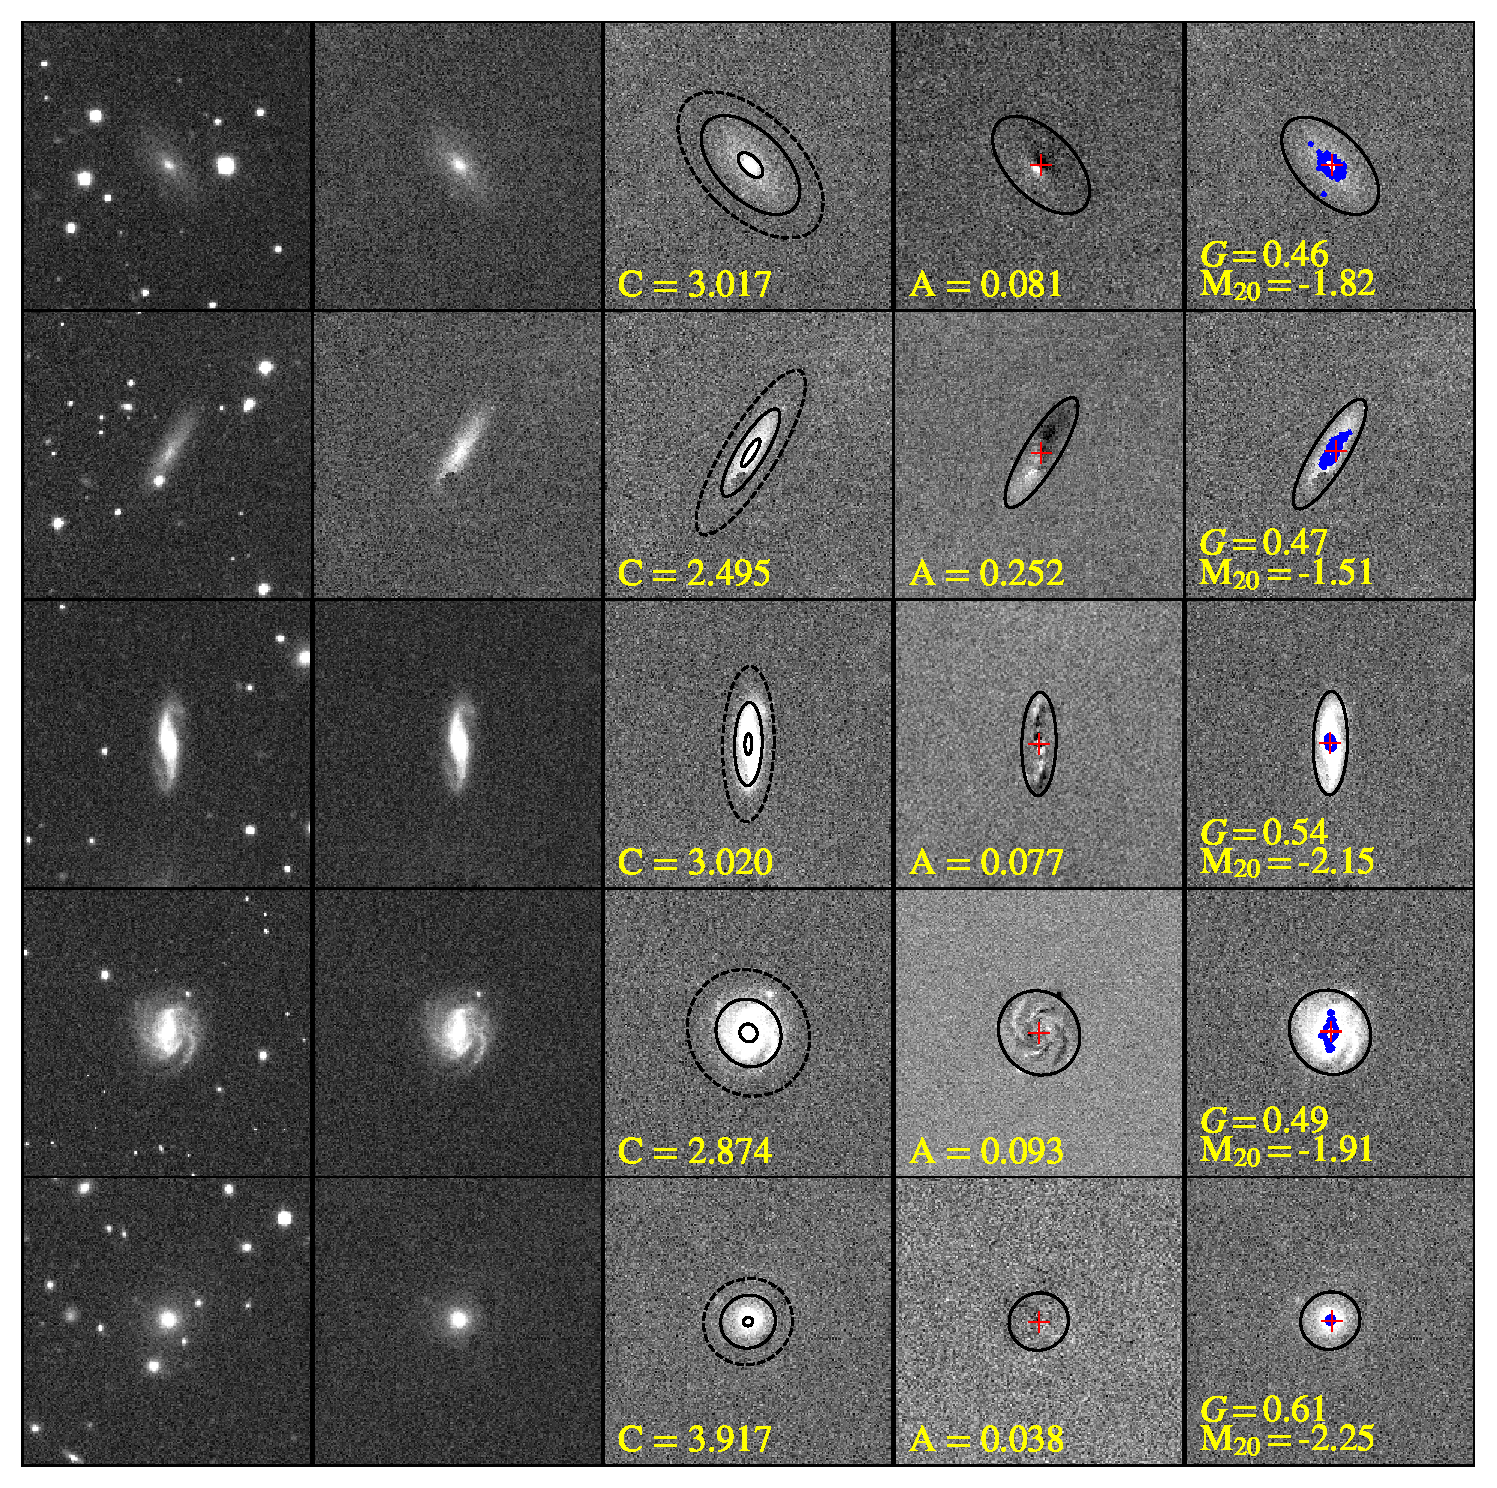
\includegraphics[width=\textwidth]{Figures/measure_morph_bin3_corrected.pdf}
\caption[Examples of image cleaning and morphology diagnostic measurements]{Additional examples of the postage stamp cleaning and morphology diagnostic measuring processes. See caption from Figure \ref{fig: morph examples}.}
\label{fig: morph examples 2}
\end{figure}

\begin{figure}
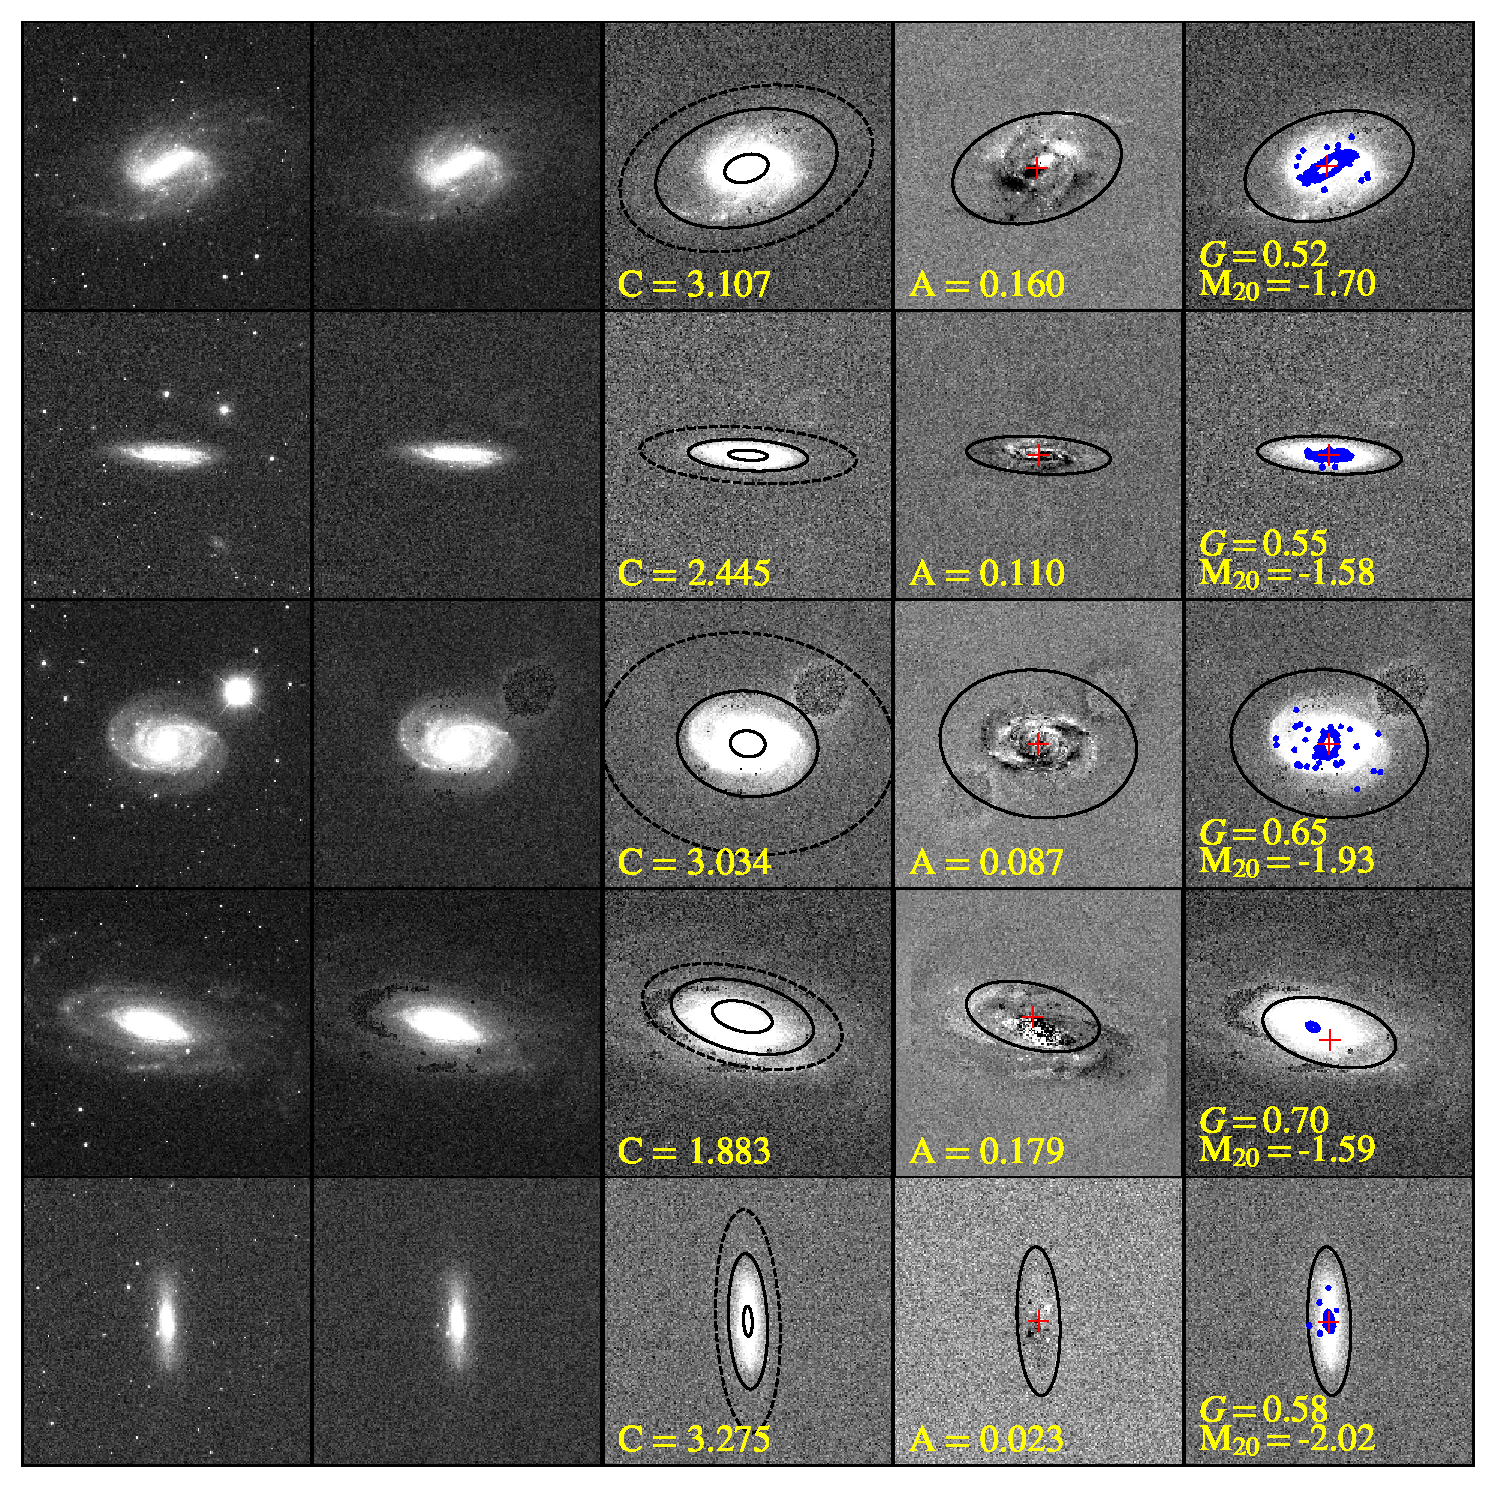
\includegraphics[width=\textwidth]{Figures/measure_morph_hardest.pdf}
\caption[Examples of image cleaning and morphology diagnostic measurements]{Examples of the postage stamp cleaning and morphology diagnostic measuring processes for a random sample of the largest and most difficult galaxies. See caption from Figure \ref{fig: morph examples}.}
\label{fig: morph examples hardest}
\end{figure}


\subsection{Morphology indicators}

Defining the flux associated with a galaxy is a challenging task: galaxies do not have constant radial surface brightness, hard edges, or uniform shapes.  Additionally, a prescription is required that measures a constant fraction of the total light while mitigating biases due to galaxy position and distance.  To combat these issues, it is common practice to use the \cite{Petrosian1976} system which computes a radius defined by the empirical shape of the galaxy's light profile. Specifically, the Petrosian radius, \rp, is such that the ratio of the surface brightness at \rp~to the mean surface brightness within \rp~is equal to a fixed value $\eta$, i.e., 

\begin{equation}\label{fig: petrosian raidus}
\eta = \frac{\mu(r_p)}{\bar\mu(r<r_p)}
\end{equation}
where $\eta$ is traditionally set to 0.2. Because this is a ratio of surface brightnesses, cosmological factors are diminished. 

We compute \rp~by first generating a set of elliptical annuli centered on the galaxy and equidistant in logspace. At least 20 annuli are used for each postage stamp. Elliptical apertures minimize the contribution from noisy background pixels. The position angle and galaxy center are taken from the SExtractor catalogs generated ealier. For each annulus, $\mu(r_i)$ is computed as the flux within the annulus divided by the annulus area, while $\mu(r<r_i)$ is computed as the total flux integrated to the center of that annulus divided by $\pi r_i^2$. This provides a crude estimate of $\eta$ which is then interpolated onto a finer set of radial values.  \rp~is that radius for which $\eta$ intersects 0.2. Examples of surface brightness profile are shown in Figure XXX. XX demonstrates a case in which the cleaning algorithm did not fully remove nearby contaminating light from other sources, resulting in an $\eta$ that never crosses the 0.2 threshold. To correct for this, we model the excess light in the outer component with a linear relation and subtract a constant value from the surface brightness profile. Even with these measures, some failures persist, however, we are only unable to obtain \rp~for 16 galaxies, a vanishingly small fraction of our sample. Using our measured values of \rp, we compute the following morphology diagnostics in an elliptical aperture with semimajor axis of one Petrosian radius. 


%\subsubsection{Concentration}
Concentration is defined in several slightly different ways with the aim being to measure the ratio of the light within an inner aperture to that within an outer aperture. Small values of this ratio typically indicate disky galaxies, while larger values correlate with early-type ellipticals. We use the definition of \cite{Bershady2000}:

\begin{equation}\label{eqn: concentration}
C = 5\log\Big(\frac{r_{80}}{r_{20}}\Big) 
\end{equation}
where \rr{80} and \rr{20} are the radii containing 80\% and 20\% of the total galaxy light respectively where we define the total flux as that within \rp~and the galaxy center is that determined by the asymmetry minimization \cite[described below,][]{Lotz2004}. A random sample of concentration measurements can be seen in the middle column of \Cref{fig: morph examples,fig: morph examples 2,fig: morph examples hardest}. 

The asymmetry parameter, $A$, quantifies the degree of rotational symmetry in the galaxy light distribution, though not necessarily the physical shape of the galaxy, as $A$ is not highly sensitive to low surface brightness features. $A$ is measured by subtracting the galaxy image rotated by 180$^{\circ}$ from the original image itself. A correction for background noise is applied \citep[as in e.g.,][]{Conselice2000, Lotz2004}, i.e., 
\begin{equation}\label{eqn: asymmetry}
A = \frac{\sum_{x,y} |I(i,j) - I_{180}(i,j)|}{ 2\sum|I(i,j)|} - B_{180}
\end{equation}
where $I$ is the galaxy flux in each pixel $(x, y)$, $I_{180}$ is the image rotated by 180 degrees about the galaxy's central pixel, and $B_{180}$ is the average asymmetry of the background. $A$ is summed over all pixels within \rp~of the galaxy's center and then normalized by a corresponding measure in the original image. The center is determined by minimizing $A$ as described in \cite{Conselice2000}. Briefly, an initial central pixel is chosen and $A$ computed. Then asymmetry is calculated again in a $3\times3$ grid about that central pixel. If one of these produces a lower value of $A$, it becomes the new center and the process repeats until a minimum is found. This is a crucial step as \cite{Conselice2000} find that a small difference can change the asymmetry by up to 50\%. Additionally, the effects due to noise must also be corrected. This is accomplished by generating a ``background cutout'': an image with the same pixel area as defined for the measurement of $A$ wherein each pixel is assigned a random value based on the statistics of the background in the original image as defined by the SExtractor segmentation maps. $A$ is computed as before, including the minimization, and this value then constitutes $B_{180}$. A random sample displaying the apertures and asymmetry centers are shown in the fourth columns of\Cref{fig: morph examples,fig: morph examples 2,fig: morph examples hardest}. 

The Gini coefficient, $G$, has long been used in econometrics as a measure of inequality by estimating the concentration of wealth in a nation's population. It is based on the Lorenz curve \citep{Lorenz1905} which is constructed by mapping the cumulative proportion of the population ranked by wealth onto the corresponding cumulative proportion of the size of their wealth. More formally, if $X$ is a positive random variable with cumulative distribution function $F(x)$ then the Lorenz curve goes as   
\begin{equation}
L(p) = \frac{1}{\bar X}\int^p_0 F^{-1}(u)~du,
\end{equation}
where $p$ is the percentile of the poorest denizens, and $\bar X$ is the mean over all values of $X_i$, a random deviate drawn from $X$. $G$ is then a summary statistic of this curve describing the mean of the absolute difference between all combinations of $X_i$:

\begin{equation}
G = \frac{1}{2\bar Xn(n-1)}\sum_{i=1}^n\sum_{j=1}^n\Big|X_i - X_j\Big|.
\end{equation}
This statistic was first applied to the distribution of a galaxy's light by \cite{Abraham2003} and further developed by \cite{Lotz2004}. In these terms, $G$ is 0 when the galaxy's flux is distributed homogeneously among all assigned pixels, and 1 if the light is concentrated within a single pixel. $G$ can be calculated more efficiently if the $X_i$ are first sorted into increasing order and then computing \citep{Glasser1962}
\begin{equation}
G = \frac{1}{|\bar X|n(n-1)}\sum_i^n(2i-n-1)|X_i|,
\end{equation}
where $n$ is the number of pixels assigned to the galaxy. Here we follow \cite{Lotz2004} by taking the absolute value of the flux, $X_i$, because in pixels with low signal-to-noise the flux is scattered to values below the mean sky level resulting in negative flux values for the faintest pixels. 

Assigning pixels to each galaxy must be given due consideration. As \cite{Lotz2004} point out, including too many sky pixels will systematically increase $G$, while exclusion of low surface brightness galaxy pixels will decrease $G$. \cite{Abraham2003} measure $G$ for pixels above a given surface brightness threshold but this will fall prey to cosmological effects. In this work, we compute $G$ from all pixels within \rp. This will exclude some low surface brightness features, especially for galaxies with faint, extended elements. However, this definition puts every galaxy on equal footing, and as we discuss in Chapter \ref{chap:4}, systematics are easily handled by the machine learning algorithm we exploit. The last column in \Cref{fig: morph examples,fig: morph examples 2,fig: morph examples hardest} shows examples of $G$.

%\subsubsection{M$_{20}$}
\M{20} is the second order moment of the brightest 20\% of the galaxy flux \citep{Lotz2004}. It traces the spatial distribution of any bright galactic features such as nuclei, bars, spiral arms, or star-forming clusters. It is computed by first calculating the total moment as
\begin{equation}
 M_{\mathrm{tot}} = \sum_i^n M_i = \sum_i^nf_i[(x_i-x_c)^2 + (y_i-y_c)^2] 
\end{equation}
where $f_i$ is the flux in pixel $x_i$, $y_i$, and $x_c$, $y_c$ is the galaxy's center which is determined by minimizing $M_{tot}$ in a similar fashion as is done for the asymmetry. The galaxy pixels are then ranked by flux in descending order and $M_i$ is summed over the brightest pixels until that sum equals 20\% of the total galaxy flux, normalized by $M_{\mathrm{tot}}$:
\begin{equation}
 M_{20} = \log_{10} \Big( \frac{\sum_iM_i}{M_{\mathrm{tot}}} \Big), ~~\textrm{while} \sum_if_i < 0.2f_{\mathrm{tot}}
\end{equation}
where $f_{tot}$ is the total flux defined within \rp. For centrally concentrated objects, \M{20} correlates with $C$ but is also sensitive to bright off-center knots of light. 

It's worth noting that both \M{20} and $G$ are correlated with $C$, but with key differences. Because $G$ is a measure of concentration it correlates strongly with $C$, especially for local galaxies \citep{Abraham2003}. However, $G$ is independent of spatial distribution: whereas $C$ measures the concentration in the central region of a galaxy, $G$ is sensitive to any concentration of light: centralized or not. M$_{20}$ takes this a step further with its key difference being a strong $r^2$ dependence. It is strongly weighted by the spatial distribution of bright regions but these need not be centralized either.  Indeed, when $G$ and \M{20} are taken together they are highly adept at identifying merging galaxies \citep{Lotz2004,Lotz2008}.  


%\subsubsection{Ellipticity}
For our final morphology diagnostic, we use the ellipticity, $\epsilon = 1 - b/a$, of the light distribution as measured by SExtractor which computes the semi-major axis $a$ and semi-minor axis $b$ from the second-order moments of the galaxy light. The ellipticity of a galaxy correlates strongly with edge-on galaxies. 

In total, we successfully measure all morphological indicators for 281,801 SDSS galaxies. Some galaxies are lost at each stage of the measurement process due to various failures which we discuss in detail below. For example, if our measurement of the Petrosian radius is not successful, no morphology diagnostics are computed for that galaxy. The number of galaxies with successful measuremenets at each stage is listed in Table \ref{tab:morph numbers}.  The relations between these diagnostics for the full sample is shown in Figure~\ref{fig: morph thresh}. The code developed to clean and compute these morphology indicators is open source and can be found at \url{https://github.com/melaniebeck/measure_morphology}.

% From the Selecting Random Subsamples for Thesis Chap3 (jupyter notebook)
\begin{table*}[]
	\centering
	\caption[Summary of morphology measurements (UPDATE THIS)]{}
	\label{tab:morph numbers}
	\let\mc\multicolumn
	\begin{tabular}{lccc}
		\mc4c{ \textbf{Morphology measurement summary}} \\
		\hline \hline
			&	&	&	\\
								  & Number &  \% Success & Notes \\
		\hline
		Full Galaxy Zoo 2 sample  	& 295 305 &	   &  \\
		Postage stamps 				& 282 350 &		95.6 	&  \% of full sample\\
		Petrosian radius			& 282 334 &		99.99 	& \% of postage stamps\\
		Concentration				& 281 927 &		99.85 	& \% of postage stamps\\ 	
		Asymmetry 					& 282 334 &		99.99 	& \% of postage stamps\\
		Gini coefficient			& 282 323 &		99.99	& \% of postage stamps\\
		M$_{20}$					& 282 194 &		99.94 	& \% of postage stamps\\	
		Ellipticity ($1 - b/a$)		& 282 350 &		100.0 	& \% of postage stamps\\
		\hline
		All morphologies successful & 281 801  &	95.4	& \% of full sample \\
	\end{tabular}
\end{table*}

\subsection{Quality and consistency}
We perform several checks to determine the quality and consistency of our morphology diagnostics. Due to the wealth of information provided by the SDSS pipeline, we can compare some of our diagnostics against SDSS values. Obviously there are some instances where our measurements will outperform the SDSS pipeline and vice versa. We first check our values of the Petrosian radius as shown in Figure \ref{fig: Rp and C comparison}. Our \rp~are on average $\sim$35\% larger than those computed by SDSS. The biggest reason for this discrepancy is due to aperture shape: SDSS compute \rp~using circular annuli while we use elliptical. [Mention the weird ones where our \rp~is tiny but SDSS's is huge? Show some examples where my code does better than SDSS? And where mine fails?]

\begin{figure}
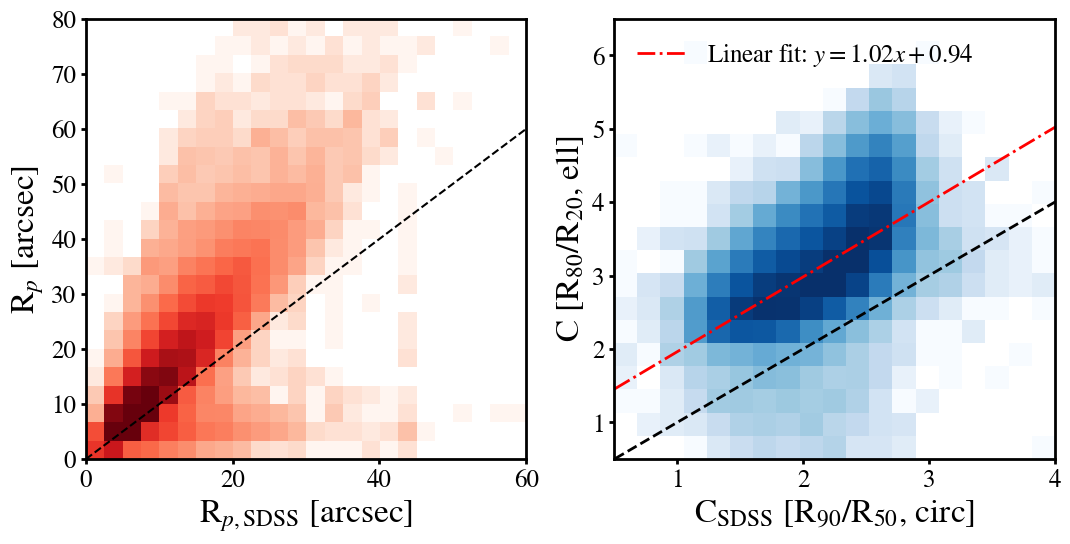
\includegraphics[width=\textwidth]{Figures/compare_Rp_concentrations.png}
\caption[Comparison of Petrosian radius and concentration index from this work to SDSS values]{Comparison of our measured \rp~and $C$ to SDSS values. In both panels the black dashed line represents a 1-to-1. The left panel shows the Petrosian radius we measure against that computed in the SDSS pipeline. Most of the discrepancy is due to the apertures used: the SDSS pipeline defines \rp~in circular annuli while we use elliptical. 
The right panel shows the relationship between concentration indexes, where the red dash-dotted line is a linear fit. We find that our $C$ is systematically $\sim$1 point larger than SDSS. This is remarkable considering $C_{\mathrm{SDSS}}$ is computed using Petrosian radii containing 50\% and 90\% of the total galaxy light while we use radii containing 20\% and 80\%, in addition to the disperate aperture shapes already mentioned.}
\label{fig: Rp and C comparison}
\end{figure}

Of greater importance, however, are the values of the morphology diagnostics as these are used as features to train our machine learning algorithm in Chapter \ref{chap:4}. Though SDSS does not measure all of the structural indicators we tackle here, they do provide a means to compute the concentration index via \texttt{PETROR50} and \texttt{PETROR90}, the Petrosian radii containing 50\% and 90\% of the galaxy total light, respectively. Figure \ref{fig: Rp and C comparison} shows our $C$ against that computed from SDSS, $C_{\mathrm{SDSS}}$. Our values are systematically $\sim$1 point larger than SDSS values but otherwise retain a strikingly tight correlation. This is suprising considering the drasticly different ways these values are computed. Besides the obvious difference in radii (SDSS uses 50\% and 90\% vs our 20\% and 80\%), SDSS values are measured using ciruclar aperture,s whereas we use elliptical. The latter is preferable as it has been shown that aperture shape affects $C$ such that the concentration index is artificially inflated when measured within circular apertures, especially for highly elongated galaxies, i.e., edge-on disks \citep{Bershady2000, Andrae2011}.


%This is hinted at in the right panel of Figure \ref{fig: concentrations} which shows the ratio $C$/$C_{\mathrm{SDSS}}$ as a function of galaxy elongation.  Instead Figure \ref{fig: concentrations} shows the opposite, that is, there exists a trend towards higher $C$ for less elongated galaxies. These are predominantly early-type galaxies (as evidenced by the $C$-$e$ panel in Figure \ref{fig: morphs as a fcn of fsmooth}). The scatter to lower $C$ is due to face-on disk galaxies. That we see the correct trend in $C$ with elongation is due to the fact that we use elliptical apertures to compute $C$ and thus our $C$ values are less prone to aperture bias.

\begin{figure}
\centering
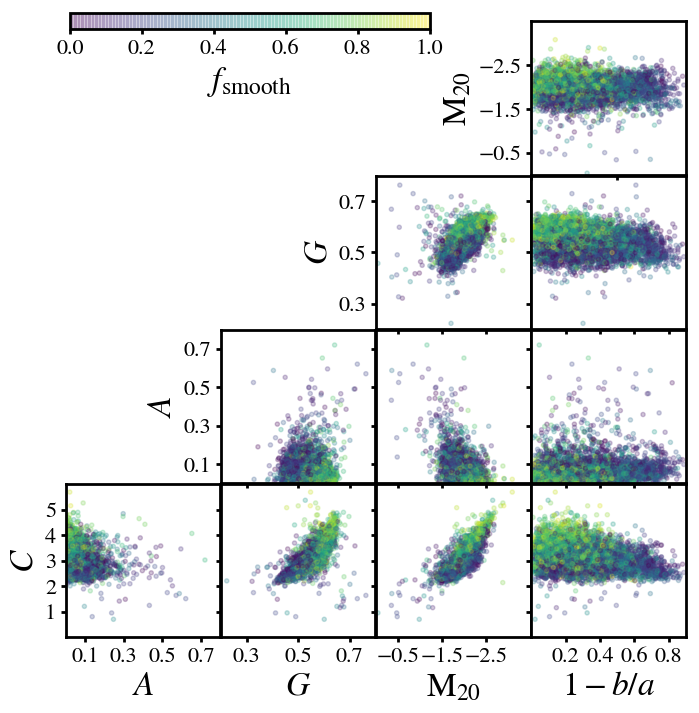
\includegraphics[width=5in]{Figures/morph_params_random_sample_fsmooth_colored_clean.png}
\caption[Automated morphologies as a function of Galaxy Zoo 2 \fsmooth]{Here a random sample of 5000 galaxies are plotted in every possible planar combination of our morphology structural indicators where the color denotes the galaxy's debiased \fsmooth~fraction from GZ2. As expected, galaxies with higher \fsmooth~are found in locations where early-types are typically seen: notably they have larger $C$ and $G$, and smaller \M{20}.}
\label{fig: morphs as a fcn of fsmooth}
\end{figure}

SDSS does not provide any other direct morphology diagnostics comparable to what we measure here so we next assess the quality of our structural indicators by estimating the fraction that are poorly measured. We consider the galaxy central coordinates assigned at various stages during the cleaning and measuring process and compare those to the original SDSS galaxy coordinates. SExtractor assigns galaxy central coordinates for each postage stamp based on the first order moment of light. Additionally, the $A$ and \M{20}~measurements each determine their own galaxy center via the minimization of their respective quantity and thus do not necessarily overlap. We compute the coordinate difference in arcseconds for each of these three centers as compared to the SDSS coordinates and determine that only 1.8\%, 1.4\%, and 0.9\% of galaxies have SExtractor, $A$, and \M{20} centers, respectively, that differ by more than $1.4\arcsec$ (the SDSS PSF) from the original SDSS coordinates. We thus find very good agreement between SDSS and SExtractor galaxy centers, indicating that we correctly identify the galaxy of interest in each postage stamp. We also find good agreement between SDSS and both the $A$ and \M{20} centers indicating that our minimizing algorithm fails in only a handful of instances.  

%Though all of these morphological diagnostics are subject to resolution, signal-to-noise, and aperture size and shape variability, the Gini coefficient is arguably the most susceptible to such issues \citep{Lisker2008}. 

Finally we consider the overall distribution of our measured structural indicators. It is well known that different galaxy types live in different parts of morphology parameter space \citep{Abraham1996,Abraham2003,Conselice2000,Lotz2004,Lotz2008}. For example, in the $G$-\M{20} plane, early-type galaxies are typically found in the upper right with late-type galaxies residing in the lower left, and merging systems in the upper left. Similar relations exist in the $C$-$G$, and $G$-\M{20}~planes. In Figure \ref{fig: morphs as a fcn of fsmooth}~we select a random sample of, for clarity, 5000 galaxies and plot them in each possible planar combination of our morphology diagnostics where the points are colored according to their Galaxy Zoo 2 debiased \fsmooth~fraction. Because \fsmooth~correlates well with early-type galaxies we see the expected trends discussed above. 



\section{Catalog of morphology diagnostics}
Below we present an excerpt of the catalog of morphology diagnostics we measured and described in this chapter. The full catalog is available ... Where??

\begin{deluxetable}{lccccccccc}
\rotate
\tablecolumns{10}
\tablewidth{0pt}
\tablecaption{Morphology Diagnostics for $\sim$283K SDSS Galaxies in the GZ2 Sample}
\tablehead{
	\colhead{DR7 objID} &
	\colhead{RA ($^{\circ}$)}	&
	\colhead{DEC ($^{\circ}$)}	&
	\colhead{R$_p$ ($\arcsec$)}	&
	\colhead{$C$}		&
	\colhead{$A$}		&
	\colhead{$G$}		&
	\colhead{\M{20}}	&
	\colhead{e}			&
	\colhead{flag}		
}
\startdata
587725550667628769 & 145.05811 & 60.57904 & 7.688 & 3.843 & 0.024 & 0.604 & -2.169 & 1.050 & 0 \\
587722984438300950 & 211.61574 & 0.84794 & 5.436 & 2.817 & 0.173 & 0.590 & -1.857 & 1.375 & 0 \\
587722982285574398 & 199.63151 & -0.84205 & 6.236 & 3.377 & 0.048 & 0.595 & -2.040 & 1.332 & 0 \\
587722982300188997 & 233.01370 & -0.83720 & 7.520 & 3.085 & 0.006 & 0.568 & -1.903 & 1.372 & 0 \\
587725550664220860 & 133.98611 & 55.43282 & 4.611 & 3.089 & 0.059 & 0.581 & -1.784 & 1.228 & 0 \\
587725083580367045 & 153.43677 & -2.12333 & 17.687 & 2.865 & 0.054 & 0.500 & -2.014 & 2.599 & 0 \\
587725471212044550 & 146.47262 & 60.21963 & 6.118 & 3.281 & 0.057 & 0.577 & -2.097 & 2.040 & 0 \\
587725474417868988 & 151.83835 & 60.88533 & 11.891 & 3.394 & -0.024 & 0.531 & -2.219 & 1.519 & 0 \\
587725471211389091 & 144.04851 & 59.35270 & 8.090 & 2.529 & 0.051 & 0.512 & -1.906 & 2.744 & 0 \\
587722982813204559 & 178.52952 & -0.42060 & 8.073 & 3.581 & -0.007 & 0.595 & -2.083 & 1.099 & 0 \\
587725550136459379 & 171.90446 & 65.68197 & 19.407 & 2.420 & 0.003 & 0.496 & -1.890 & 5.162 & 0 \\
587722983362134374 & 206.06578 & -0.00380 & 7.243 & 3.024 & 0.048 & 0.583 & -2.266 & 2.596 & 0 \\
587725082507870286 & 156.26072 & -3.02887 & 10.261 & 2.681 & 0.024 & 0.504 & -1.822 & 1.224 & 0 \\
587725471206670541 & 129.87227 & 52.06361 & 12.570 & 3.477 & 0.043 & 0.539 & -2.197 & 1.437 & 0 \\
587725040100704461 & 200.04925 & -2.82914 & 7.173 & 3.432 & 0.039 & 0.590 & -1.943 & 1.246 & 0 \\
587725550143668309 & 210.94442 & 63.89091 & 4.833 & 2.963 & 0.058 & 0.556 & -1.869 & 1.096 & 0 \\
587725075528941624 & 139.16755 & 0.42750 & 17.521 & 2.841 & 0.092 & 0.517 & -2.037 & 3.459 & 0 \\
%587724649256452276 & 178.59272 & -2.69328 & 7.472 & 2.169 & 0.022 & 0.423 & -1.576 & 1.458 & 0 \\
%587724650337206457 & 194.62813 & -1.83056 & 8.575 & 3.363 & 0.018 & 0.559 & -2.104 & 1.057 & 0 \\
\enddata
\end{deluxetable}

\label{tab: morphologies}


\begin{figure}
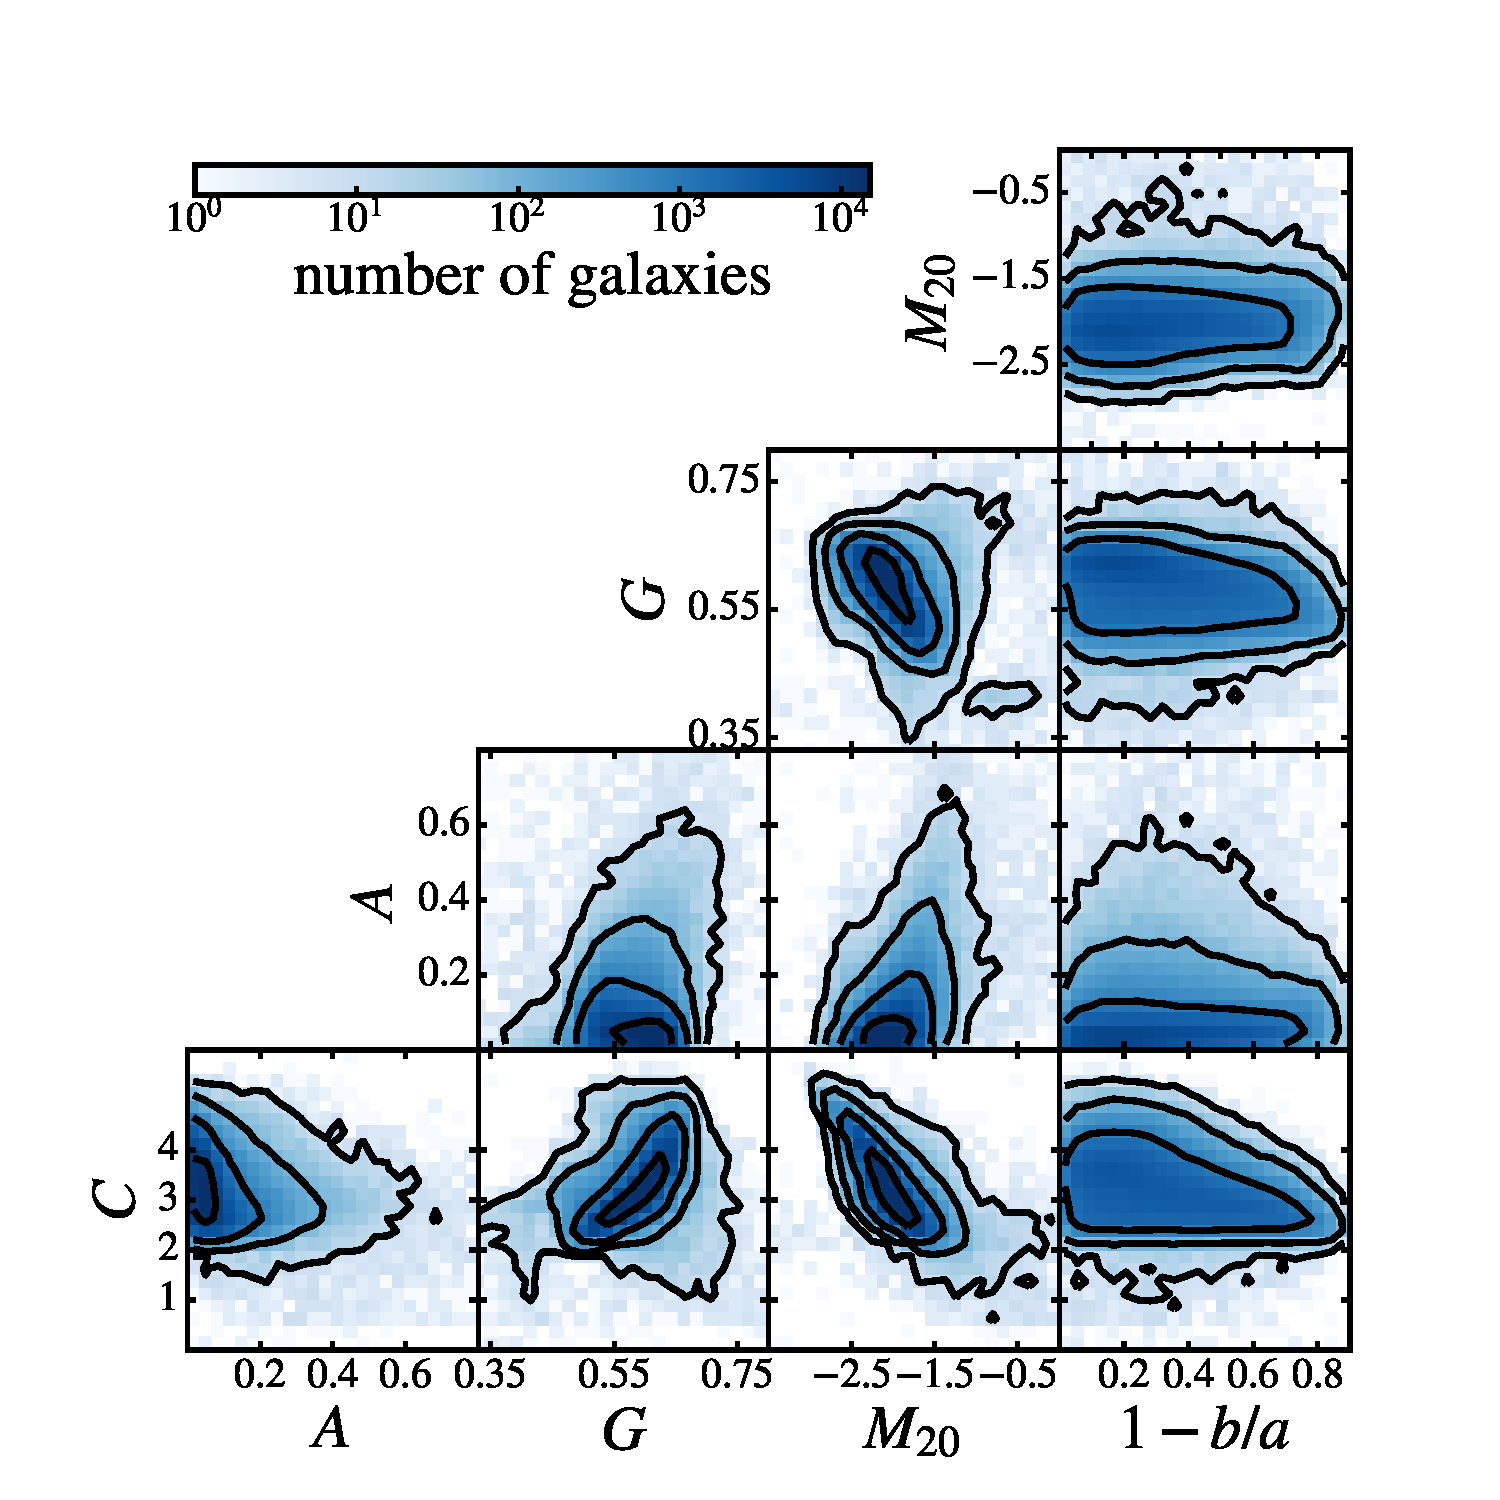
\includegraphics[width=\textwidth]{Figures/human_machine/A2b.pdf}
\caption[Automated morphologies for the full GZ2 sample.]{Relation between measured morphology diagnostics for more than 280K SDSS galaxies. Correlations between several diagnostics are immediately obvious and not all relations are likely to be linear. These points will be revisited in Chapter \ref{chap:4} when we discuss machine learning algorithms.}
\label{fig: morphs}
\end{figure}
%!TEX root = thesis.tex

\chapter{Intelligent management of visual classifications}
\label{chap:3}


%%----------------------------------------------------------------------------------------------------------------------------------------------------
%%   Galaxy Zoo 2 Data Description
%%---------------------------------------------------------------------------------------------------------------------------------------------------
\section{Galaxy Zoo 2 Classification Data} \label{sec: data}

Our simulations utilize original classifications made by volunteers during the GZ2 project. These data\footnote{\url{data.galaxyzoo.org}} are described in detail in~\cite{Willett2013} and the preceding Chapter, though we provide a brief overview here.  The GZ2 subject sample consists of 285,962 galaxies identified as the brightest 25\% ($r$-band magnitude $< 17$) residing in the SDSS North Galactic Cap region from Data Release 7 and included subjects with both spectroscopic and photometric redshifts out to $z < 0.25$. Subjects were shown as colour composite images via a web-based interface\footnote{\url{www.galaxyzoo.org}} wherein volunteers answered a series of questions pertaining to the morphology of the subject. With the exception of the first question, subsequent queries were dependent on volunteer responses from the previous task creating a complex decision tree\footnote{A visualization of this decision tree can be found at \url{https://data.galaxyzoo.org/gz_trees/gz_trees.html}}. Using GZ2 nomenclature, a \textit{classification} is the total amount of information about a subject obtained by completing all tasks in the decision tree. A subject is \textit{retired} after it has achieved a sufficient number of classifications.
%\footnote{\url{zoo2.galaxyzoo.org}}


For our current analysis, we choose the first task in the tree: ``Is the galaxy simply smooth and rounded, with no sign of a disk?" to which possible responses include ``smooth", ``features or disk", or ``star or artifact". This choice serves two purposes: 1) this is one of only two questions in the GZ2 decision tree that is asked of every subject thus maximizing the amount of data we have to work with, and 2) our analysis assumes a binary task and this question is simple enough to cast as such. Specifically, we combine ``star or artifact" responses with ``features or disk" responses.

We assign each subject a descriptive label in order to validate our classification output with GZ2. GZ2 classifications are composed of volunteer vote fractions for each response to every task in the decision tree, denoted as $f_{\mathrm{response}}$. They are derived from the fraction of volunteers who voted for a particular response and are thus approximately continuous. A common technique is to place a threshold on these vote fractions to select samples with an emphasis on purity or completeness, depending on the science case. For our current analysis we choose a threshold of 0.5, that is, if \ffeat+\fstar~$ >$ \fsmooth, the galaxy is labelled~\feat, otherwise it is labelled~\notfeat. We note that only 512 subjects in the GZ2 catalogue have a majority \fstar, contributing less than half a percent contamination when combining the ``star or artifact" with ``features or disk" responses.

The GZ2 catalogue publishes three types of vote fractions for each subject: raw, weighted, and debiased. Debiased vote fractions are calculated to correct for redshift bias, a task that GZX does not perform. The weighted vote fractions account for inconsistent volunteers. The SWAP algorithm (described below) also has a mechanism to weight volunteer votes, however, the two methods are in stark contrast. For consistency, we thus derive labels from the raw vote fractions (\raw); those that have received no post-processing whatsoever. In total, the data consist of over 14 million classifications from 83,943 individual volunteers. 

The labels we compute from GZ2 vote fractions are used solely to validate our classification method and are thus considered ``ground truth,'' though this is, of course, subjective. Furthermore, we envision our framework being applied to never-before-classified image sets for which ``ground truth" labels would not yet exist. Nevertheless, in Appendix XXX we show how different choices of our descriptive GZ2 labels change the perceived quality of our classification system and demonstrate that our method yields robust galaxy classifications.


%%-----------------------------------------------------------------------------
%%   Talk About SWAP 
%%-----------------------------------------------------------------------------
\section{Efficiency through intelligent human-vote aggregation}\label{sec: SWAP}

Galaxy Zoo 2 had a brute-force subject retirement rule whereby each galaxy was to receive approximately forty independent classifications.  Once the project reached completion, inconsistent volunteers were down-weighted~\citep{Willett2013}, a process that does not make efficient use of those who are exceptionally skilled. To intelligently manage subject retirement and increase classification efficiency, we adapt an algorithm from the Zooniverse  project Space Warps~\citep{Marshall2016}, which searched for and discovered several gravitational lens candidates in the CFHT Legacy Survey~\citep{More2016}.  Dubbed SWAP (Space Warps Analysis Pipeline), this algorithm computed the probability that an image contained a gravitational lens given volunteers' classifications and experience after being shown a training sample consisting of simulated lensing events.  We provide a brief overview here.  

The algorithm assigns each volunteer an \textit{agent} which interprets that volunteer's classifications. Each agent assigns a 2$\times$2 confusion matrix to their volunteer which encodes that volunteer's probability to correctly identify feature \A~given that the subject exhibits feature \A; and the probability to correctly identify the absence of feature \A~(denoted \N) given that the subject does not exhibit that feature. The agent updates these probabilities by estimating them as 

\begin{equation}
P(``X" | X, \mathbf{d}) \approx \frac{\mathcal{N}_{``X"}}{\mathcal{N}_{X}}
\end{equation}
where $X$ is the true classification of the subject and ``$X$" is the  classification made by the volunteer upon viewing the subject. Thus $\mathcal{N}_{``X"}$ is the number of classifications the volunteer labelled as type $X$, $\mathcal{N}_X$ is the number of subjects the volunteer has seen that were actually of type $X$, and $\mathbf{d}$ represents the history of the volunteer, i.e., all subjects they have seen. Therefore the confusion matrix for a single volunteer goes as

\begin{eqnarray}
\mathcal{M} & = & \left[
	\begin{array}{cc}
		P(``A"|N, \mathbf{d}) ~~& P(``A" | A, \mathbf{d}) \\[0.3em]
		P(``N"|N, \mathbf{d})~~& P(``N"|A, \mathbf{d}) \\[0.3em]
	\end{array}\right]
\end{eqnarray}
where probabilities are normalised such that $P(``A"|A) = 1- P(``N" | A) $.

Each subject is assigned a prior probability that it exhibits feature \A: $P(A) = p_0$. When a volunteer makes a classification, Bayes' theorem is used to compute how that subject's prior probability should be updated into a posterior using elements of the agent's confusion matrix. As the project progresses, each subject's posterior probability is updated after every volunteer classification, nudged higher or lower depending on volunteer input. Upper and lower probability thresholds can be set such that when a subject's posterior crosses the upper threshold it is highly likely to exhibit feature \A; while if it crosses the lower threshold it is highly likely that feature \A~is absent. Subjects whose posteriors cross either of these thresholds are considered retired.


\subsection{Gold-standard sample}\label{sec: training sample}

A key feature of the original Space Warps project was the training of individual volunteers through the use of simulated images. These were interspersed with real imaging and were predominantly shown at the beginning of a volunteer's association with the project, allowing that volunteer's agent time to update before classifying real data. Volunteers were provided feedback in the form of a pop-up comment after classifying a training image. GZ2 did not train volunteers in such a way, presenting a challenge when applying SWAP to GZ2 classifications. Though we cannot retroactively train GZ2 volunteers, we develop a gold standard sample and arrange the order of gold standard classifications in order to mimic the Space Warps system.


We create a gold standard sample by selecting 3496 SDSS galaxies representative of the relative abundance of T-Types, a numerical index of a galaxy's stage along the Hubble sequence, at $z\sim0$ by considering galaxies that overlap with the~\cite{NairAbraham2010} catalogue, a collection of $\sim$14K galaxies classified by eye into T-Types. We generate expert labels for these galaxies that are consistent with the labels we defined for GZ2 classifications. These are obtained through the Zooniverse platform\footnote{The Project Builder template facility can be found at \url{http://www.zooniverse.org/lab.}} from 15 professional astronomers, including members of the Galaxy Zoo science team.  The question posed was identical to the original top-level GZ2 question and at least five experts classified each galaxy. Votes are aggregated and a simple majority provides an expert label for each subject. This ensures that our expert labels are defined in exactly the same manner as the labels we assign the rest of the GZ2 sample. Our final dataset consists of the GZ2 classifications made by those volunteers who classify at least one of these gold standard subjects. We thus retain for our simulation 12,686,170 classifications from 30,894 unique volunteers. When running SWAP, classifications of gold standard subjects are always processed first. 

\subsection{Volunteer Bias}

\begin{figure}
\centering
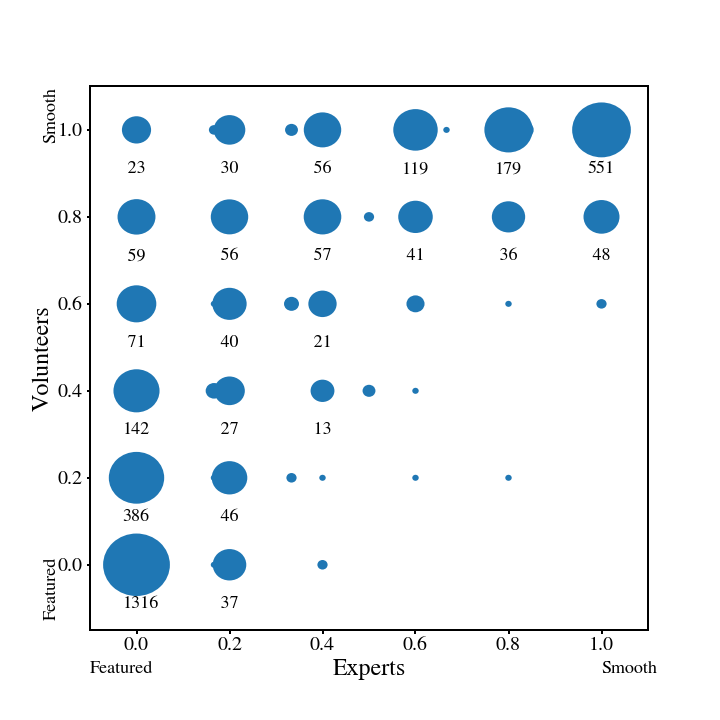
\includegraphics[width=5in]{Figures/expert_vs_volunteer_votes_highskill_11-6-17.png}
\caption[]{Volunter bias of labeling galaxies `Smooth' (\notfeat) as compared to expert classifications for the gold standard sample.}
\label{fig: volunteer bias}
\end{figure}

By comparing expert and GZ2 volunteer votes we uncover indications of volunteer bias towards labeling galaxies as `Smooth' (`Not Featured'). For each galaxy in our gold standard sample we identify the five most skilled volunteers who classified that galaxy, where skill is determined by the volunteer confusion matrix in Figure \ref{fig: confusion matrix}. We compute \fsmooth~from those five volunteers. In Figure \ref{fig: volunteer bias} we plot the volunteer \fsmooth~against the expert \fsmooth~sample, where the size of the circle is proportional to the number of subjects wherein both volunteers and experts agreed. Circles representing more than ten gold standard subjects are also labelled with the correponding number of galaxies at that location in \fsmooth~space. For example, there are 1316 subjects that both experts and volunteers labeled \feat~with \fsmooth~$ = 0.0$. Though the vast majority of galaxies received five expert classifications, some received more than that resulting in blue circles at one sixth intervals instead of the majority at fifths. The large circles at $0.0$ and $1.0$ indicate that both experts and volunteers agree for more than half of the gold standard sample. However, that the circles extend almost solely into the upper left hand corner indicates that volunteers consistently label galaxies as `Smooth' moreso than experts. Of this small sample, 40\% of galaxies are given a larger \fsmooth~by volunteers than by experts. 

It is well known that redshift and surface brightness affect the apparent strength of morphological features in CCD imaging in that finer details are harder to identify. GZ2 mitigate these issues by ``debiasing'' volunteer vote fractions \citep{Willett2013}. We compare both the original raw and debiased \fsmooth~vote fractions for the gold standard sample and find that it cannot account for the pronounced bias seen here. The reason for this is unsurprising as this sample was selected from the \cite{NairAbraham2010} catalog, which consists of bright, low-redshift galaxies. Effects due to cosmic distance are thus minor. 

This then suggests that the bias could be inherent to the question posed to volunteers: ``Is the galaxy simply smooth and rounded, with no sign of a disk?'' Terminology such as ``disk'' could be misinterpreted by those without specific astrophysics training. Experienced astronomers are more adept at identifying galactic disks, even those which posses few other obvious features. On the other hand, if volunteers do not see obvious features such as spiral arms or a bar, they could well mark galaxies as ``smooth.''  A similar issue is also observed in the GZ: CANDELS project in which \cite{Simmons2017} compares volunteer classifications to expert classifications collected by the CANDELS team \citep{Kartaltepe2015}. This comparison is, however, not ideal as the question posed to the CANDELS team was not identical to that given to GZ volunteers. With the small sample presented here, it is difficult to determine how much this bias could affect the full GZ2 galaxy sample though we touch on this issue again in Chapter \ref{chap:4}. 



%%----------------------------------------------------------------------------------------------------------------------------------------------------
%%   Subsection:    		SWAP only (FIDUCIAL RUN)
%%----------------------------------------------------------------------------------------------------------------------------------------------------
\subsection{Fiducial SWAP simulation}\label{sec: fiducial}

%% ----------------------------------------------------------------------------
%%   FIGURE:  VOLUNTEER PROBABILITIES
%% ----------------------------------------------------------------------------
\begin{figure}
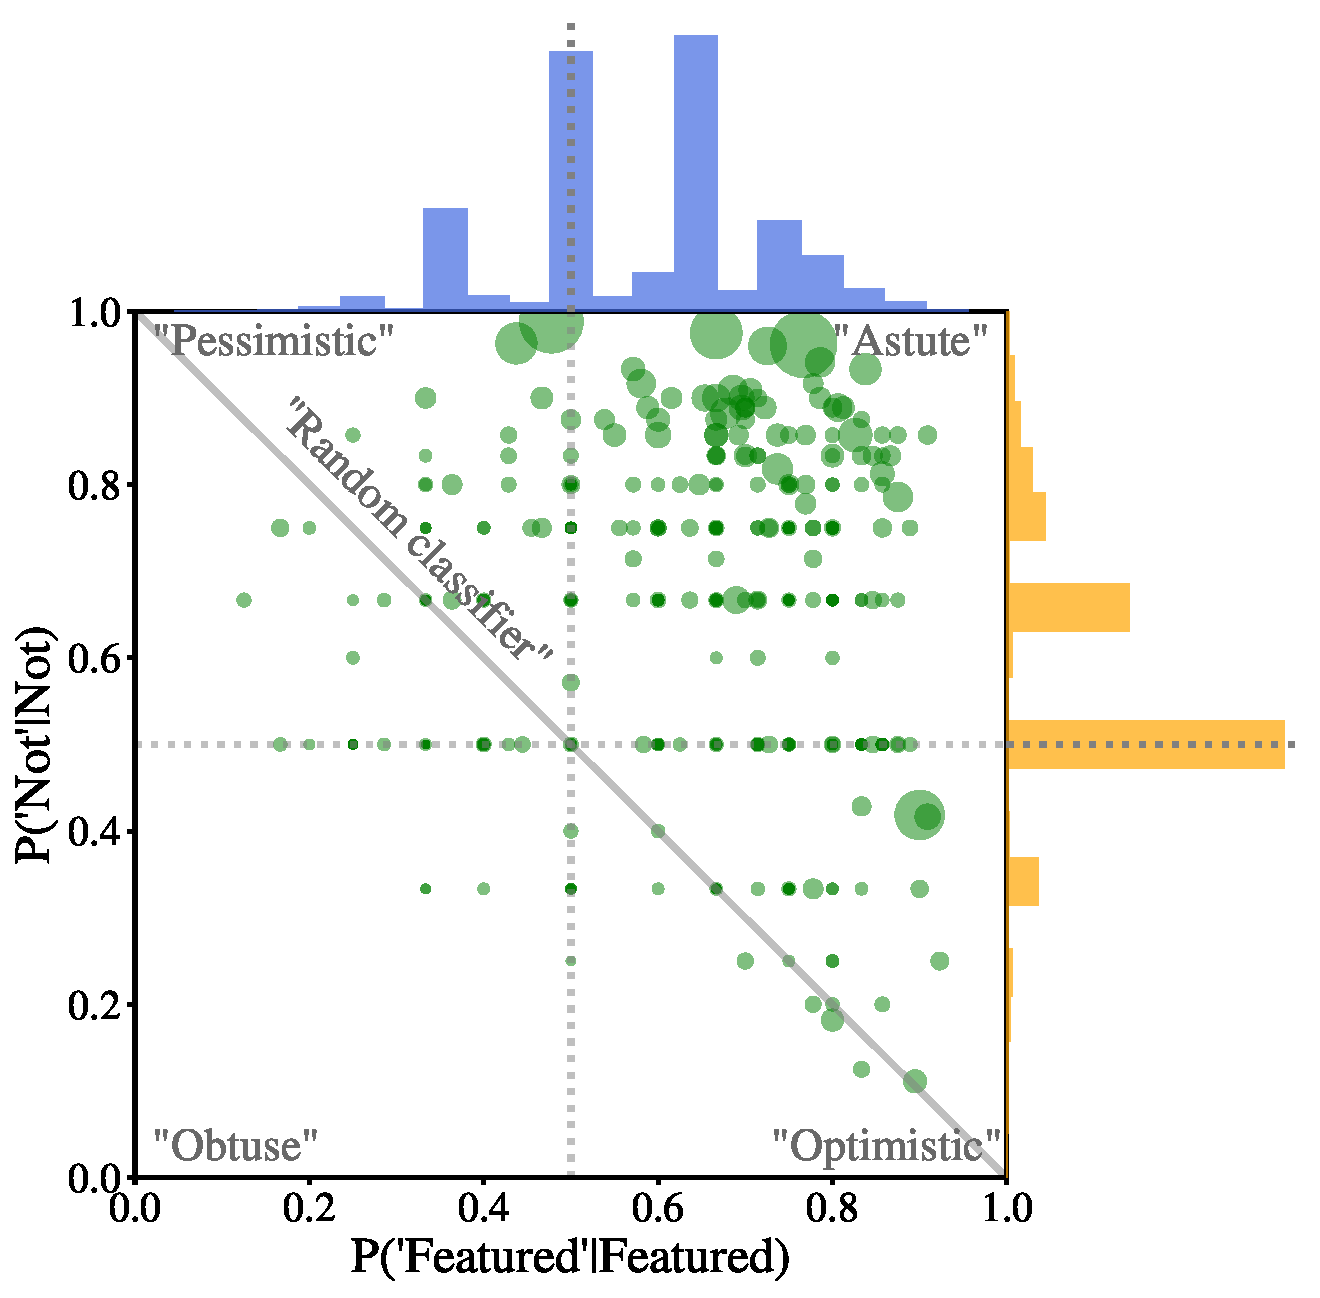
\includegraphics[width=3.45in]{Figures/human_machine/f2.pdf}
\caption[Volunteer confusion matrices achieved through SWAP reprocessing of GZ2 data.]{Confusion matrices for 1000 randomly selected GZ2 volunteers after fiducial SWAP assessment. Circle size is proportional to the number of gold standard subjects each volunteer classified. The histograms on top and right represent the distribution of each component of the confusion matrix for all volunteers.  A quarter of GZ2 volunteers are ``Astute"; they correctly identify both \feat~and \notfeat~subjects more than 50\% of the time. The peaks at 0.5 in both distributions are due primarily to volunteers who see only one training image: only half of their confusion matrix is updated.}
\label{fig: volunteer training}
\end{figure}

%%%-------------------------------------------------------
%%%  FIGURE:   SUBJECT POSTERIOR PROBABILITIES
%%%-------------------------------------------------------
\begin{figure} 
\centering
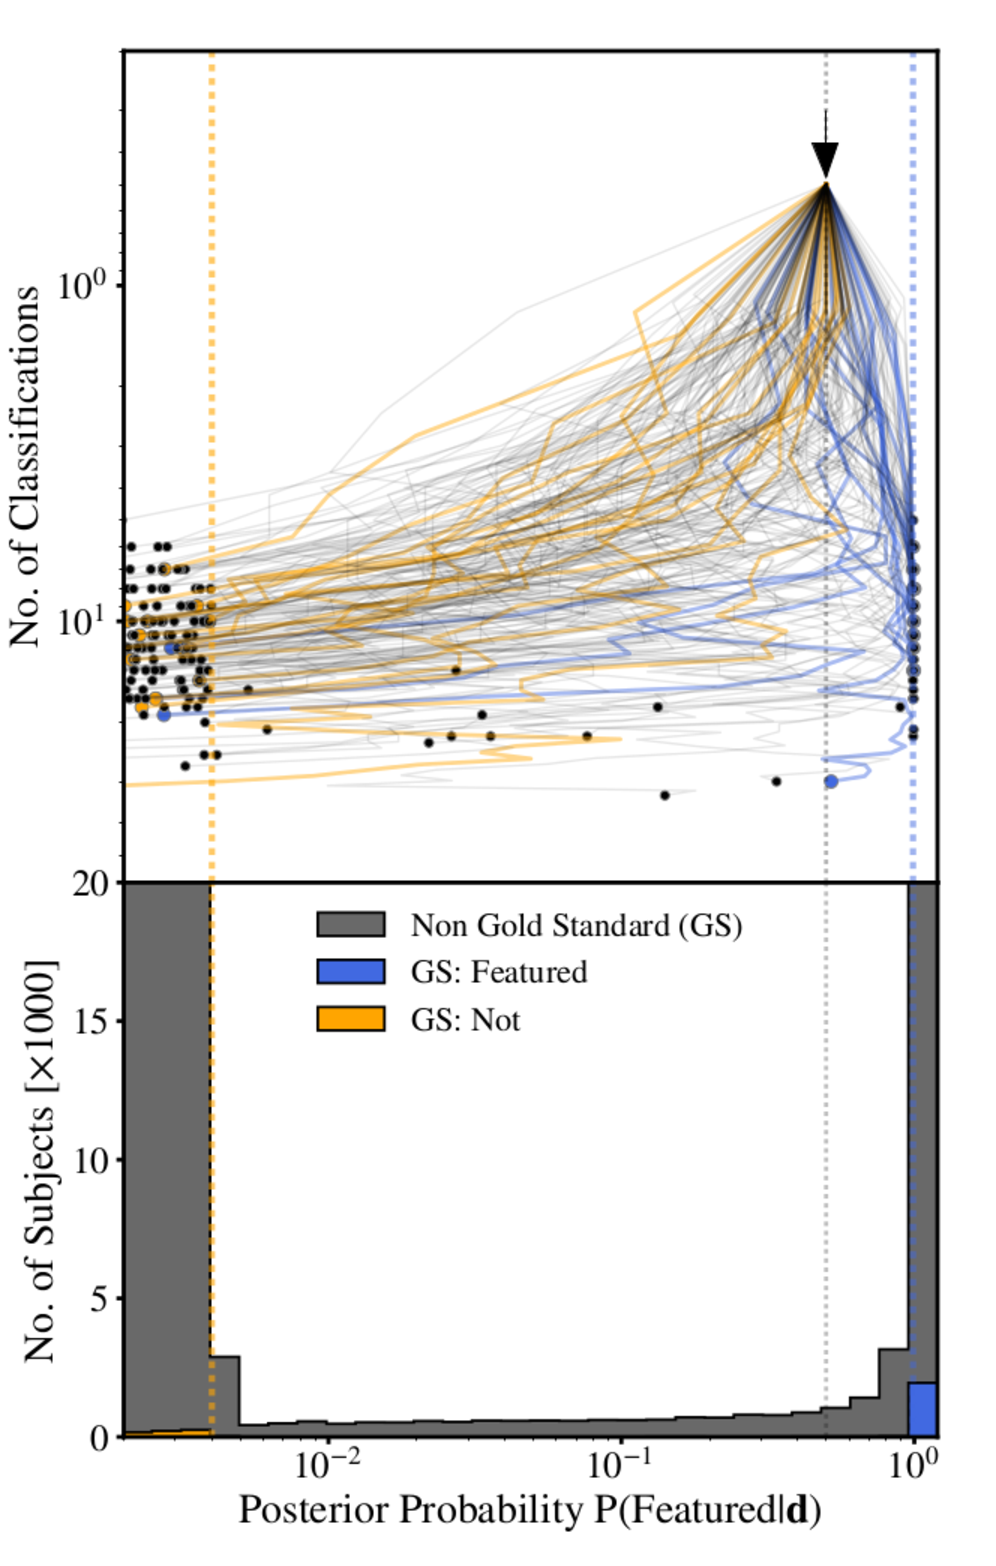
\includegraphics[width=3.25in]{Figures/human_machine/f12.pdf}
\caption[Galaxy posterior probabitilies realized through SWAP reprocessing of GZ2 data.]{Posterior probabilities for GZ2 subjects.  The top panel depicts the probability trajectories of 200 randomly selected GZ2 subjects. All subjects begin with a prior of 0.5 denoted by the arrow. Each subject's probability is nudged back and forth with each volunteer classification. From left to right the dotted vertical lines show the \notfeat~threshold, prior probability, and \feat~threshold. Different colours denote different types of subjects. The bottom panel shows the distribution in probability for all GZ2 subjects by the end of our simulation, where the y axis is truncated to show detail.}
\label{fig: subject probabilities}
\end{figure}


Before we run a simulation, a number of SWAP parameters must be chosen: the initial confusion matrix for each volunteer's agent, (\Pf, \Pn); the subject prior probability, \p; and the retirement thresholds, \tf~and \tn. For our fiducial  simulation, we initialize all confusion matrices at (0.5, 0.5), and set the subject prior probability, \p~$= 0.5$. We set the~\feat~threshold, \tf, i.e., the minimum probability for a subject to be retired as~\feat, to $0.99$. Similarly, we set the~\notfeat~threshold, \tn~$= 0.004$. In Section XXX we show that varying these parameters has only a small affect on the SWAP output. To simulate a live project, we run SWAP on a time step of $\Delta t = 1$ day, during which SWAP processes all volunteer classifications with timestamps within that range. This is performed for three months worth of GZ2 classification data. 

Figure~\ref{fig: volunteer training} (adapted from Figure 4 of~\citealt{Marshall2016}) demonstrates the volunteer assessment we achieve, and shows confusion matrices for 1000 randomly selected volunteers. The circle size is proportional to the number of gold standard subjects each volunteer classified. The histograms represent the distribution of each component of the confusion matrix for all volunteers. Nearly 25\% of volunteers are considered ``Astute"  indicating they correctly identify both \feat~and \notfeat~subjects more than 50\% of the time. Furthermore, as long as a volunteer's confusion matrix is different from random, they provide useful information to the project. The spikes at $0.5$ in the histograms are due to volunteers who see only one gold standard subject (i.e.,~\feat), leaving their probability in the other (\notfeat) unchanged. Additionally, 4\% of volunteers have a confusion matrix of (0.5, 0.5) indicating these volunteers classified two gold standard subjects of the same type, one correctly and one incorrectly. 

Figure~\ref{fig: subject probabilities} (adapted from Figure 5 of \citealt{Marshall2016}) demonstrates how subject posterior probabilities are updated with each classification. The arrow in the top panel denotes the prior probability, \p~$=0.5$. With each classification, that prior is updated into a posterior probability creating a trajectory through probability space for each subject. The blue and orange lines show the trajectories of a random sample of \feat~and \notfeat~subjects from our gold standard sample, while the black lines show the trajectories of a random sample of GZ2 subjects that were not part of the gold standard  sample. The similarly coloured vertical dashed lines correspond to the retirement thresholds, \tf~and \tn. The lower panel shows the full distribution of GZ2 subject posteriors at the end of our simulation, where the y-axis has been truncated to show detail. An overwhelming majority of subjects cross one of these retirement thresholds.

Our goal is to increase the efficiency of galaxy classification. We therefore  use as a metric the cumulative number of retired subjects as a function of the original GZ2 project time. We define a subject as GZ2-retired once it achieves at least 30 volunteer votes, encompassing 98.6\% of GZ2 subjects (explored in depth in Section XXX).  In contrast, a subject is considered SWAP-retired once its posterior probability crosses either of the retirement thresholds defined above. 

%%%-------------------------------------------------------
%%%  FIGURE:    CONFUSION MATRIX -- GZX VS GZ2
%%%-------------------------------------------------------
\begin{figure} 
\centering
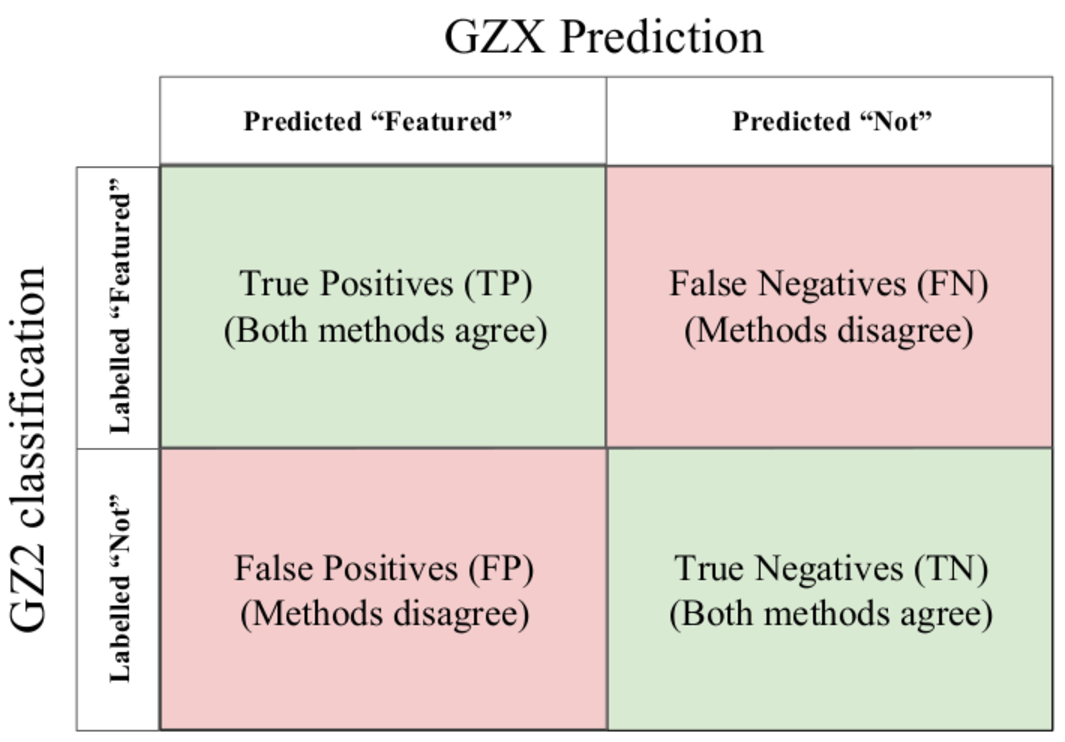
\includegraphics[width=3.2in]{Figures/human_machine/confusionmatrix.pdf}
\caption[Confusion matrix between predictions and ground truth defines quality metrics.]{Confusion matrix for comparing GZ2 classifications to our method.  True positives (TP) and true negatives (TN) indicate that the predictions from our method agree with GZ2 for subjects labelled \feat~and \notfeat, respectively. When the two classification methods disagree, the result is a sample of false negatives (FN) and false positives (FP). This allows us to easily compute  quality metrics like accuracy, completeness, and purity with respect to GZ2 as shown in Equations \ref{eqn: metrics}.} 
\label{fig: confusion matrix}
\end{figure}

However, it is important not to prioritize efficiency at the expense of quality. Because we have a binary classification we can construct a confusion matrix from which we can compute the quality metrics of accuracy, completeness and purity as a function of GZ2 project time by comparing our predicted labels to the \raw~labels. Figure \ref{fig: confusion matrix}
graphically depicts the elements of this confusion matrix. From this we compute: 
 
\begin{align*}\label{eqn: metrics}
\mathrm{accuracy} &= \frac{TP + TN}{TP + FP + TN + FN} \\
\mathrm{completeness} &= \frac{TP}{TP +FN }\tag{3} \\
\mathrm{purity} &= \frac{TP}{TP + FP}
\end{align*}

Thus, a complete sample recovers \textit{all} subjects labelled \feat~by GZ2, whereas a pure sample recovers \textit{only} subjects labelled \feat~by GZ2. For example, by Day 20, SWAP retires 120K subjects with 96\% accuracy, 99.7\% completeness, and 92\% purity. 
 
Figure \ref{fig: fiducial run} and Table~\ref{tab: summary} detail the results of our fiducial SWAP simulation compared to the original GZ2 project. The bottom panel shows the cumulative number of retired subjects as a function of GZ2 project time. By the end of our simulation, GZ2 (dashed dark blue) retires $\sim$50K subjects while SWAP (solid light blue) retires 226,124 subjects. We thus classify 80\% of the entire GZ2 sample in three months. Processing volunteer classifications through SWAP presents nearly a factor of 5 increase in classification efficiency. The top panel of Figure~\ref{fig: fiducial run} demonstrates the quality of those classifications as a function of time and establishes that our full SWAP-retired sample is 95.7\% accurate, 99\% complete, and 86.7\% pure. We discuss these small discrepancies in Section XXX.

%%%-------------------------------------------------------
%%%  FIGURE:    SWAP FIDUCIAL RUN
%%%-------------------------------------------------------
\begin{figure}
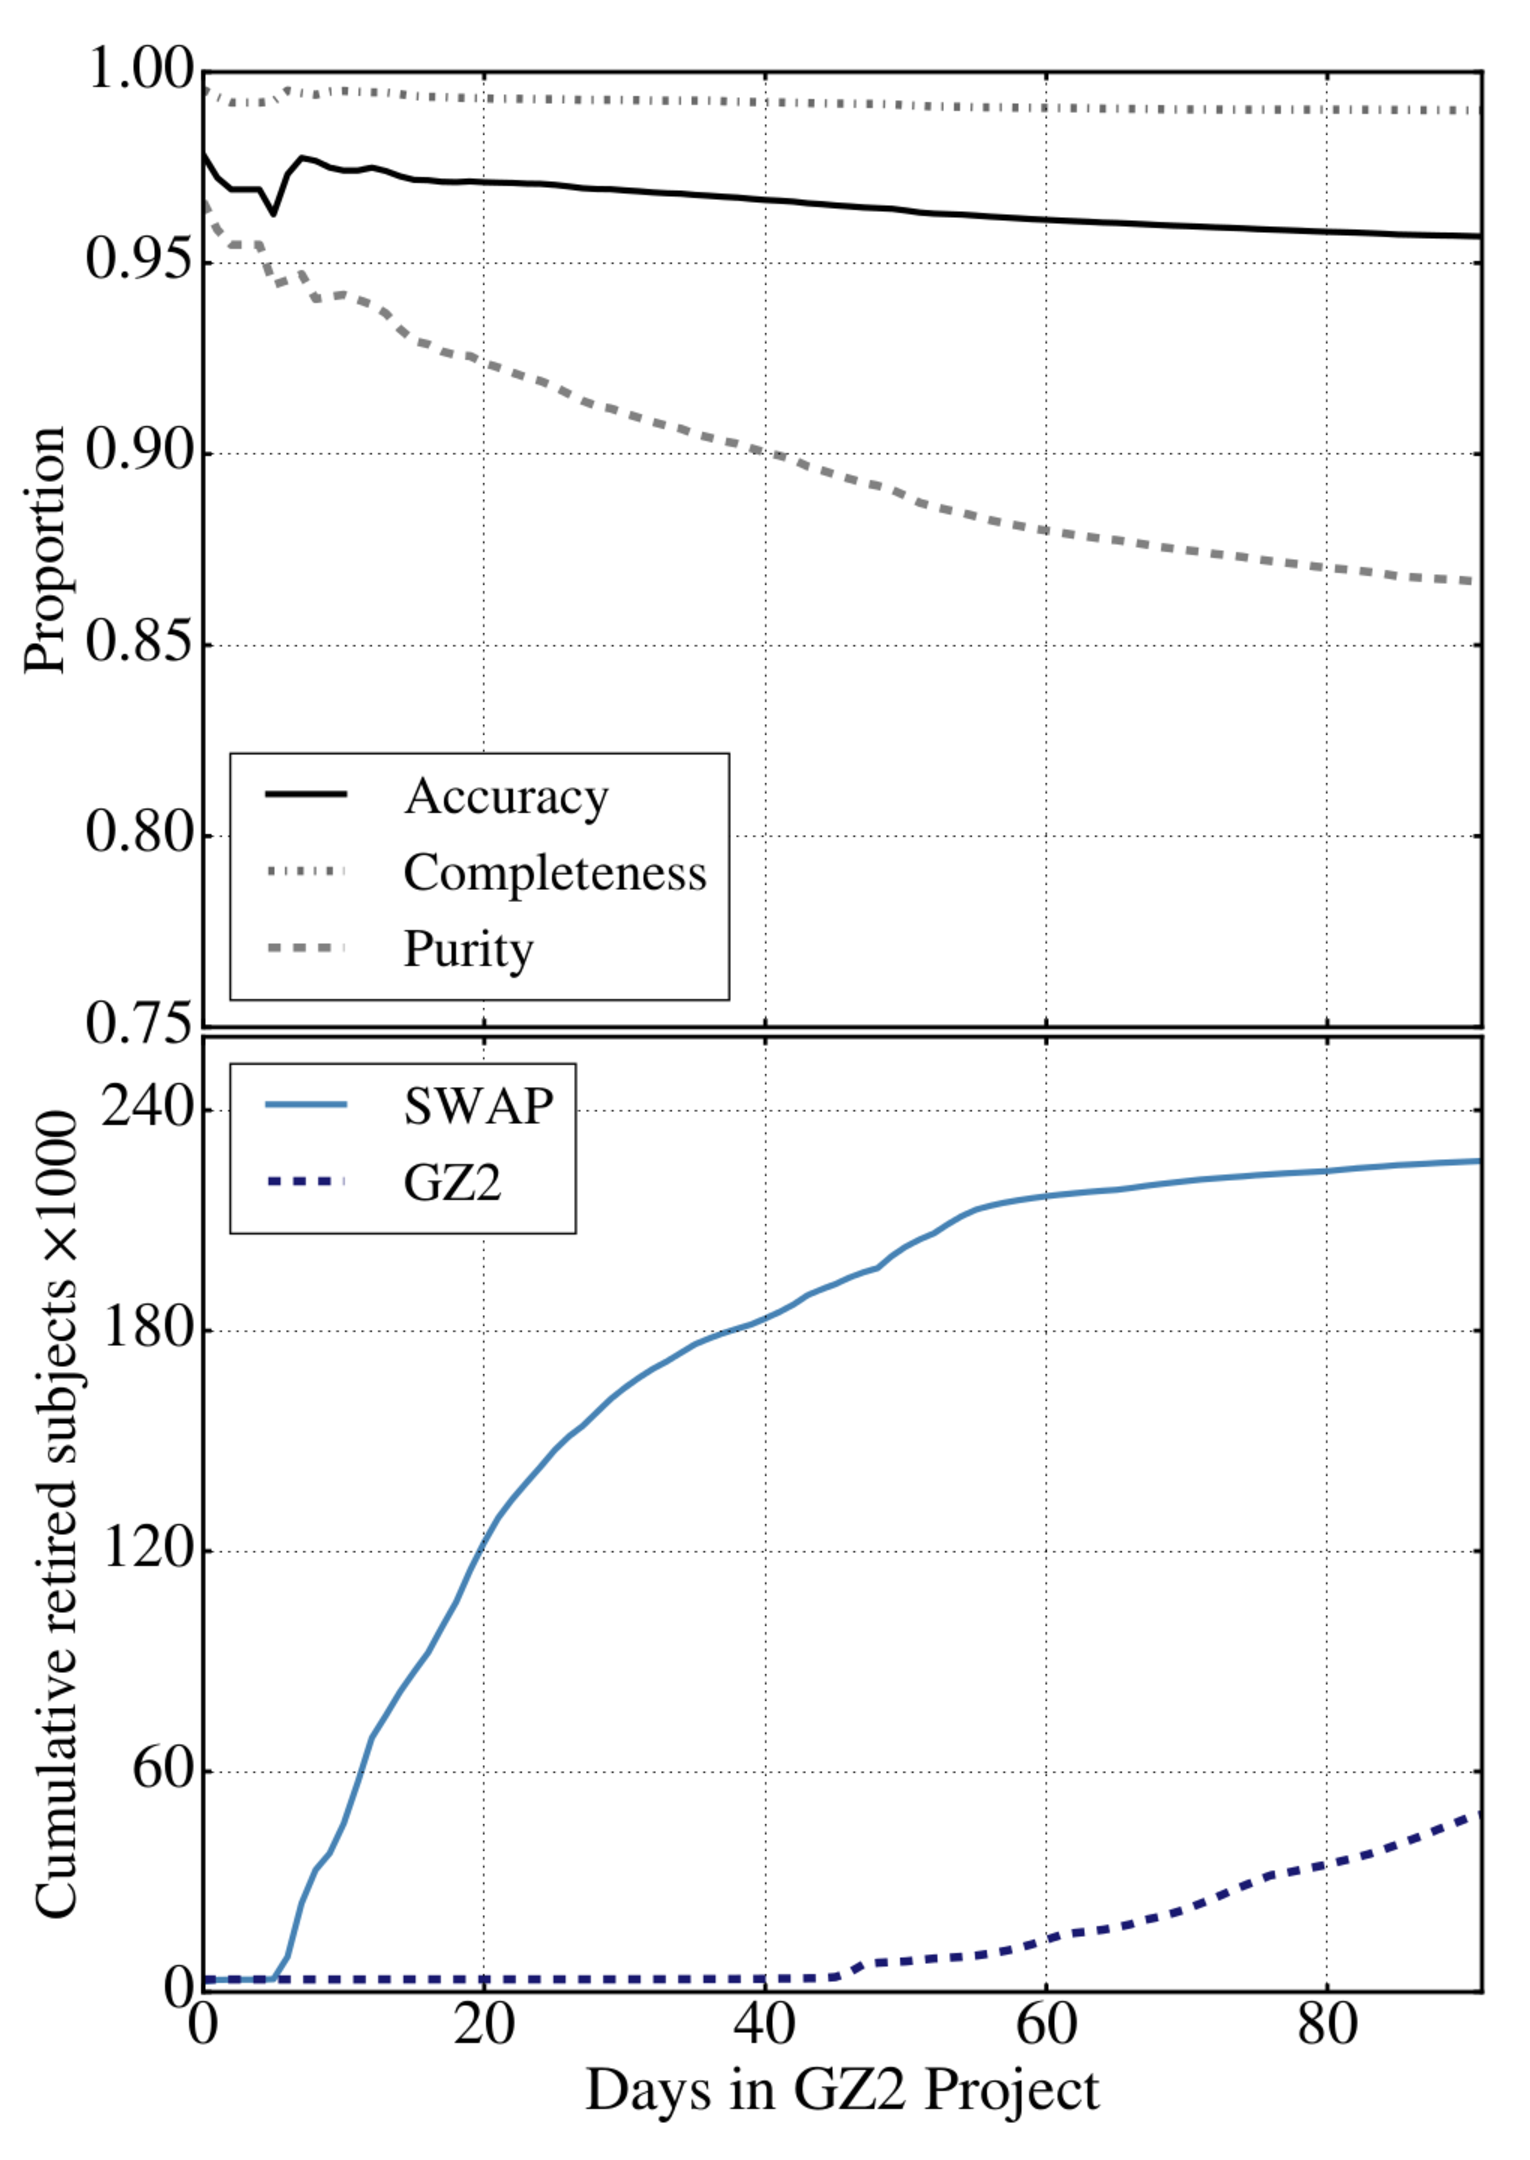
\includegraphics[width=3.35in]{Figures/human_machine/f3.pdf}
\caption[Reprocessing GZ2 data with SWAP results in a factor of increase in the classification rate.]{Fiducial SWAP simulation demonstrates a factor of 4.7 increase in the rate of subject retirement as a function of GZ2 project time (bottom panel, light blue) compared with the original GZ2 project (dashed dark blue). After 92 days, SWAP retires over 226K subjects, while GZ2 retires $\sim$48K.  The top panel displays the quality metrics (greys). These are calculated by comparing labels predicted by SWAP to~\raw~labels (Section~\ref{sec: data}) for the subject sample retired by that day of the simulation. Thus, on the final day, SWAP retires 226,124 subjects with 95.7\% accuracy,  and with completeness and purity of~\feat~subjects at 99\% and 86.7\% respectively. The decrease in purity as a function of time is due, in part, to the fact that more difficult to classify subjects are retired later in the simulation (see Section~\ref{sec: swap is faster}).}
\label{fig: fiducial run}
\end{figure}


%%%--------------------------------------------------------------------------------------------------
%%%  SECTION:   SWAP IS FASTER THAN GZ2 SANS DECISION TREE
%%%--------------------------------------------------------------------------------------------------
\subsection{Intelligent subject retirement}\label{sec: swap is faster}

That SWAP achieves a classification rate nearly 5 times faster than GZ2 comes with a caveat: we consider only the top-level question of the GZ2 decision tree, which, it can be argued, required that GZ2 secure enough votes to populate the subqueries.  In order to put SWAP and GZ2 on equal footing we determine the minimum number of votes, $N$, that the GZ2 project would need to achieve the same top-level classification for 95\% of its sample.

\begin{figure}
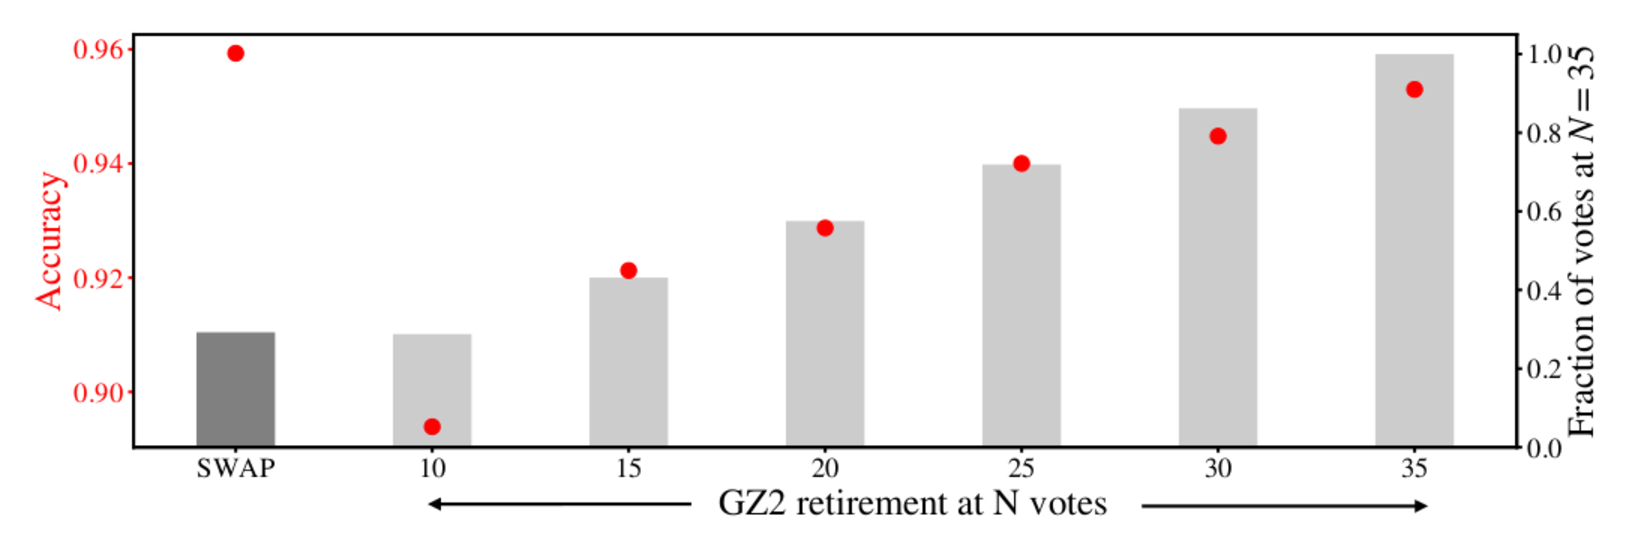
\includegraphics[width=\linewidth]{Figures/human_machine/f15.pdf}
\caption[SWAP's intelligent retirement mechanism 3.5 times fewer classifications than GZ2.]{SWAP's intelligent retirement mechanism allows it to use 30\% fewer classifications than GZ2 for the top-level question. To see this, we determine the minimum number of votes GZ2 needs in order to achieve consistent top-level classifications 95\% of the time, allowing us to compare the total number of votes in our SWAP simulation to the total number required for GZ2. We compute the vote fractions \fsmooth, \ffeat, and \fstar~using only the first $N$ votes in GZ2 and then compute the resulting class label.  We compare these labels to those we originally computed in Section~\ref{sec: data} using the full GZ2 vote fractions and compute the accuracy and the total number of votes necessary for subject retirement. We do this for 100 randomly selected subsamples from GZ2 with the same number of subjects as retired during our SWAP simulation. The red dots show the average accuracy while the grey bars denote the average fraction of votes compared to that required for $N=35$ (statistical error bars on these quantities are too small to be seen.) GZ2 needs at least 35 votes per subject in order to retain consistent subject classifications for 95\% of the GZ2 sample. SWAP can surpasses this accuracy using only 30\% as many votes.}
\label{fig: gz2 min retirement}
\end{figure}

We compute the raw vote fractions (\ffeat, \fsmooth, and \fstar) for every subject in the GZ2 sample using only the first $N$ classifications for $N \in [10, 15, 20, 25, 30, 35]$. From this, we compute descriptive labels as described in Section~\ref{sec: data}. Because our SWAP simulation did not retire every subject in the GZ2 sample, we select 100 random subsamples each consisting of 226,124 subjects, and compute the average accuracy and the average number of total GZ2 classifications necessary retire that subsample. These results are shown in Figure~\ref{fig: gz2 min retirement} for each value of $N$ along with the accuracy and total classifications for our SWAP simulation. We see that GZ2 needs at least 35 votes per subject in order to achieve consistent class labels 95\% of the time.  SWAP achieves the same accuracy with 30\% fewer classifications. Furthermore, this justifies our choice of defining a subject as GZ2-retired once it reached at least 30 classifications.

SWAP's performance can be explained through its retirement mechanism. GZ2 retired subjects randomly and required an arbitrary number of classifications per subject. In contrast, SWAP retires ``easier" subjects first while harder subjects remain in the system for longer (requiring many more classifications to nudge that subject's posterior across a retirement threshold).  Evidence for this can be seen in the top two panels of Figure~\ref{fig: swap retirement}. The top left panel shows the distribution of \fsmooth~for the entire GZ2 sample (orange), the SWAP-retired sample (blue), and the sample of subjects which SWAP has not yet retired, of which there are $\sim 19$K at the end of our simulation. The SWAP-retired sample generally follows the same distribution as GZ2-full except for the noticeable dip around \fsmooth$=0.6$. In contrast, the SWAP-not-yet-retired sample peaks at \fsmooth$=0.6$. These subjects can be interpreted as being the most difficult to classify which can be understood intuitively: galaxies with \fsmooth~$\le 0.5$ are easily identified as having features, while galaxies with \fsmooth~$\ge 0.8$ are obviously elliptical.

 This is further corroborated in the top right panel which shows the distribution of the number of classifications a subject had at the time of retirement. The solid lines show this distribution from the original GZ2 project for the same subsamples as the top left panel. For comparison, the dashed line shows the number of classifications at retirement realized during our SWAP simulation. Again, we see that the SWAP-retired sample is representative of GZ2 as a whole. However, the distribution for the SWAP-not-yet-retired sample is skewed toward fewer total classifications. To understand this, consider the following: GZ2 served subject images at random with the  exception that, towards the end of the project, subjects with low numbers of classifications were shown at a higher rate to ensure that each galaxy had enough responses to accurately characterize the likelihood of the classification~\citep{Willett2013}. The median number of classifications was 44 with the full distribution shown in orange in the top right panel of Figure~\ref{fig: swap retirement}. Our SWAP simulation processes these classifications in the same order as the original project (with the exception that gold-standard subject classifications are processed first as described in Section~\ref{sec: training sample}). Because our simulations cycle through only 92 days of GZ2 data, there are three general scenarios for why a subject has not yet been retired through SWAP: 1) SWAP has seen only a few of the many classifications for a given subject and it is not yet enough to retire it, 2) SWAP has seen many of the classifications for a subject but that subject is difficult; if we ran the simulation longer to process the remaining GZ2 classifications, SWAP would eventually retire it, and 3) SWAP has seen most or all of the classifications for a subject but it is difficult and there are few or no remaining GZ2 classifications; without additional volunteer input, these subjects will never be retired by SWAP. It is this third category that skews the red distribution towards fewer GZ2 votes. These are difficult-to-classify subjects that have only 30 - 40 GZ2 classifications, all of which are processed by SWAP, but these subjects remain unretired.

We have demonstrated that SWAP retires subjects intelligently: quickly retiring easy-to-classify subjects while allowing those that are more difficult to collect additional classifications. SWAP thus needs 30\% as many votes to retire nearly 5 times as many subjects during the three months of GZ2 project time that we include in our simulation.


%%%-------------------------------------------------------
%%%  FIGURE:    SWAP IS FASTER; RETIRES EASIEST FIRST
%%%-------------------------------------------------------
\begin{figure}
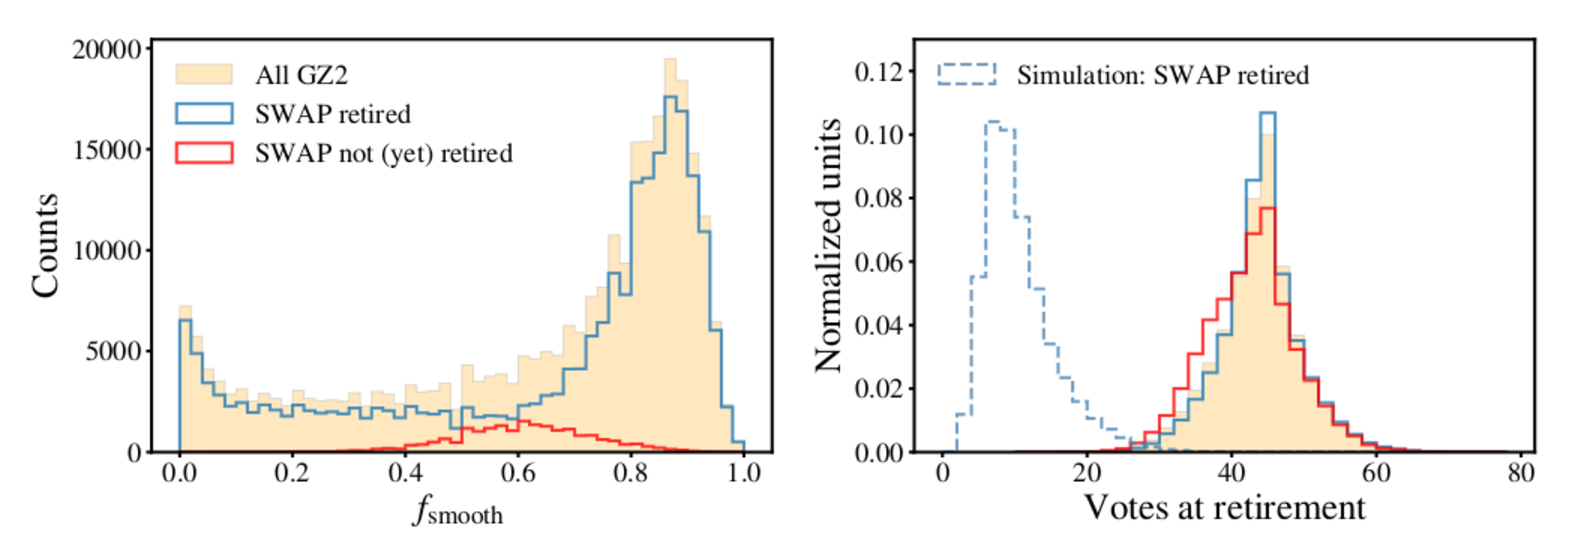
\includegraphics[width=\linewidth]{Figures/human_machine/f14.pdf}
\caption[SWAP increase classification efficiency by retiring ``easy'' galaxies quickly.]{SWAP uses 30\% fewer classifications to retire subjects due to its ability to retire easier subjects quickly, while more difficult subjects remain in the system to acquire additional classifications. The top left panel shows~\fsmooth~for the entire GZ2 sample (orange), the subjects retired by SWAP (blue), and subjects that SWAP has not yet retired by the end of our simulation (red). The latter distribution peaks at \fsmooth~$\sim 0.6$, which can intuitively be understood as the most difficult to classify subjects: those with \fsmooth~$\le 0.5$ are easily identified as \feat, while those with \fsmooth~$\ge 0.8$ are more obviously \notfeat. The top right panel provides additional evidence where here we show the number of votes at retirement for both the original GZ2 project (solid lines) and our SWAP simulation (dashed blue). The left-skew inherent in the red SWAP-not-yet-retired sample is due to difficult-to-classify subjects that received only 30-40 classifications during the GZ2 project. Even after processing all available classifications, SWAP cannot retire these subjects without additional volunteer input.}
\label{fig: swap retirement}
\end{figure}



\subsection{Reducing human effort}
SWAP's intelligent retirement mechanism is due, in large part, to how SWAP estimates volunteer classification ability which, in turn, allows for a dramatic reduction in the amount of human effort (votes) required. To see this, we consider a toy model wherein we simulate volunteers with fixed confusion matrices. We simulate 1000 \feat~subjects and 1000 \notfeat~subjects each with prior, \p~$ = 0.5$. We simulate 100 volunteer agents all with the same fixed confusion matrix of (0.63, 0.65), where these values are computed as the average \Pf~and \Pn~from our assessment of real volunteers, excluding the spikes at 0.5. We generate volunteer classifications based on this confusion matrix (i.e., volunteers will correctly identify \feat~subjects 63\% of the time) and update the subject's posterior probability with each classification. We track how many classifications are required for each subject's posterior to cross either the \feat~or \notfeat~retirement thresholds. 


%%%-------------------------------------------------------
%%%  FIGURE:   SWAP vote distributions
%%%-------------------------------------------------------
\begin{figure}
\centering
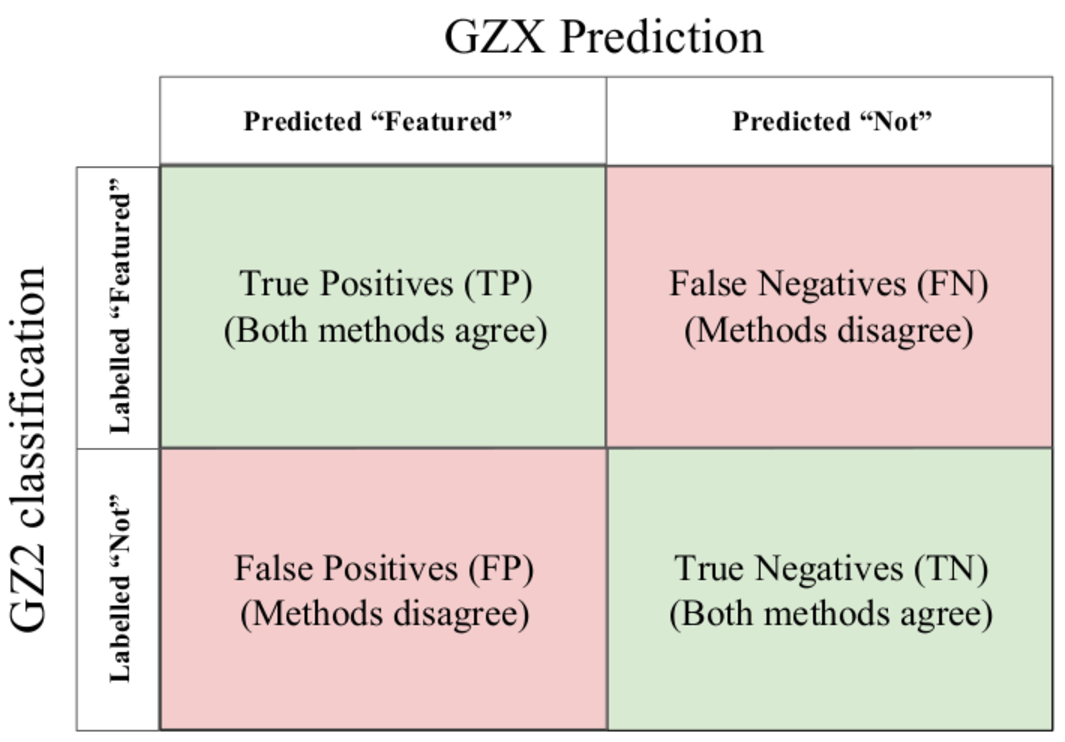
\includegraphics[width=3.5in]{Figures/human_machine/f4.pdf}
\caption[SWAP's volunteer-weighting mechanism provides a factor of three reduction in the required human effort for classification tasks.]{SWAP's volunteer-weighting mechanism provides a factor of three reduction in the human effort required to retire GZ2 subjects. The filled histograms show the number of volunteer classifications per subject achieved during our SWAP simulation broken down by class label, where the solid black line is the total. The dashed histograms are results from our toy model in which we simulate volunteers with fixed confusion matrices, effectively disengaging SWAP's volunteer-weighting mechanism. These broad distributions require $\sim$3 times more classifications per subject to reach the same retirement thresholds.} 
\label{fig: swap vote distributions}
\end{figure}

The results are presented in Figure~\ref{fig: swap vote distributions}. The filled blue and orange histograms show the number of classifications per subject achieved from our SWAP simulation, where volunteer agent confusion matrices are those from Figure~\ref{fig: volunteer training}. The dashed blue and orange distributions are the results from our toy model. When SWAP accounts for volunteer ability, most subjects are retired with between 6 and 15 votes, with a median of 9 votes. In contrast, when every volunteer is given equal weighting, subjects require 16 to 45 votes with a median of 30 votes before crossing one of the retirement thresholds. Thus the volunteer weighting scheme embedded in SWAP can reduce the amount of human effort required to retire subjects by a factor of three.

This reduction will be, in part, a function of the number of gold standard subjects each volunteer sees.  Our gold standard sample was chosen to be representative of morphology rather than evenly distributed among GZ2 volunteers. We thus find that half of our volunteers classify only one or two gold standard subjects. That we achieve a factor of three reduction when only half of our volunteer pool has seen $\ge 2$ gold standard subjects suggests that an additional reduction of  human effort is possible with more extensive volunteer training.



\subsection{Disagreements between SWAP and GZ2}\label{sec: swap gz2 disagree}

Galaxy Zoo's strength comes from the consensus of dozens of volunteers voting on each subject. Processing votes with SWAP reduces the number of classifications to reach consensus. Though we typically recover the \raw~label, SWAP disagrees about 5\% of the time. We thus examine the false positives (subjects SWAP labels as \feat~but \raw~labels as~\notfeat) and false negatives (subjects SWAP labels as \notfeat~but \raw~labels as \feat). We explore these subjects in redshift, magnitude, physical size, and concentration but find no correlation with any of these variables, suggesting that, at least for this galaxy sample, the reliability of morphology depends on factors that are not captured by these coarse measurements. This is perhaps unsurprising since GZ2 subjects were selected from the larger GZ1 sample to be the brightest, largest and nearest galaxies:  precisely those subjects most accessible for visual classification. 

%%%-------------------------------------------------------
%%%  FIGURE:   SWAP failures
%%%-------------------------------------------------------
\begin{figure}
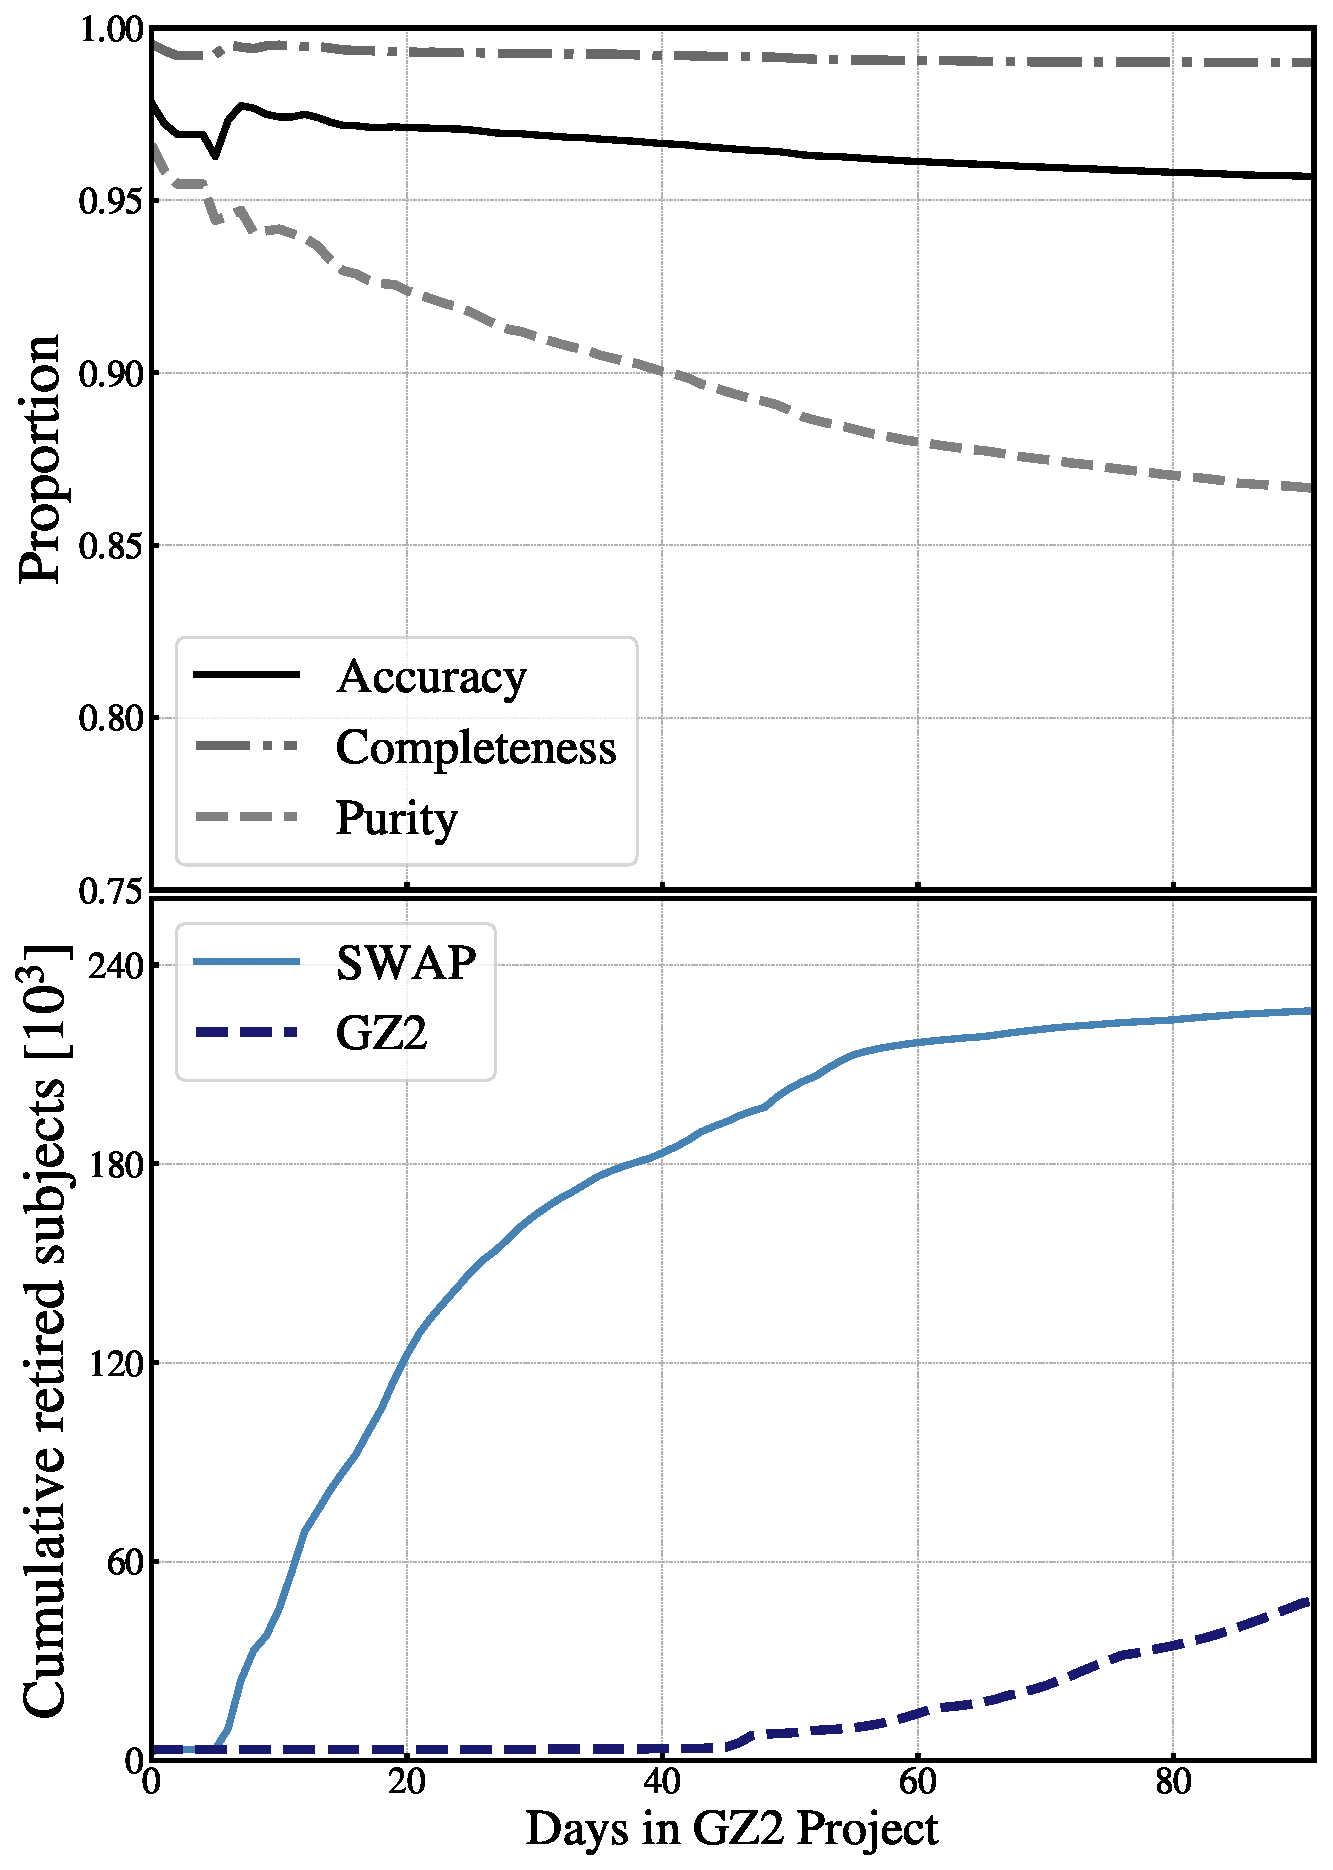
\includegraphics[width=3.5in]{Figures/human_machine/f5.pdf}
\caption[SWAP's prediction disagrees with the GZ2 label as a result of the confidence interval around the chosen threshold used to define the GZ2 label.]{Distribution of GZ2 \ffeat+\fstar~vote fractions for subjects correctly identified by SWAP (dotted grey), along with those identified as false positives (solid purple), and false negatives (dashed teal). 
The false positives and false negatives are scaled by factors of 10 and 100 respectively for easier comparison. From Section~\ref{sec: data}, subjects with values $> 0.5$ are defined as~\feat, however, the teal distribution indicates that SWAP labels them as~\notfeat. This is not a flaw of SWAP: 68.9\% of incorrectly identified subjects have $0.4 \le $~\ffeat +\fstar~$ \le 0.6$ suggesting that~\raw~labels are simply too uncertain. The overlap between the false positives and negatives is due to subjects that are exactly 50-50; by default these are labelled~\notfeat.}
\label{fig: SWAP sucks}
\end{figure}

Instead we consider the stochastic nature of GZ2 vote fractions, which can be estimated as binomial. Let success be a response of ``smooth'' and failure be any other response. The $68\%$ confidence interval on a subject with \fsmooth~$=0.5$ is then $(0.42, 0.57)$ assuming 40 classifications, each with a probability of 0.5. Figure~\ref{fig: SWAP sucks} shows the distribution of \ffeat+\fstar~for the false positives (solid purple), and the false negatives (dashed teal) compared to the  subjects where SWAP and GZ2 agree (dotted grey).  Recall that if this value is greater than 0.5, the subject is labeled \feat. The majority of disagreements between SWAP and GZ2 are for subjects that have $0.4 <$~\ffeat+\fstar~$< 0.6$. It is thus unsurprising that SWAP and GZ2 disagree most within the approximate confidence interval of our selected GZ2 threshold. We note that the distribution overlap between false positives and false negatives is due to subjects that do not have a majority; these are labeled \notfeat~by default. 

Two other effects contribute to the disagreement between SWAP and GZ2. First, as the number of classifications used to retire a galaxy decreases, the likelihood of misclassification by random chance increases. Second, disagreement arises due to expert-level volunteers whose confusion matrices are close to 1.0. These volunteers are essentially more strongly weighted, allowing that subject's posterior to cross a retirement threshold in as few as two classifications. In rare cases, despite training, some expert-level 
volunteers get it wrong compared to the gold-standard labels. These issues can be mitigated by requiring each subject reach a minimum number of classifications in addition to its posterior probability crossing a retirement threshold, thus combining the best qualities of GZ2 and SWAP. 


\subsection{Summary}

%In Appendix~\ref{sec: tweaking swap}, we find that varying the initial SWAP 
%parameters from the fiducial values does not substantially change the results 
%presented here. The largest influence comes from choosing unrealistic subject 
%prior probabilities, which can mildly degrade the quality of the resulting classifications. 
%More importantly, none of these effects significantly alters our human and machine integration in Section~\ref{sec: results}. 


We demonstrate nearly a factor of five increase in the classification rate, a reduction of at least a factor of three in the human effort necessary to maintain that increased rate, all while maintaining 95\% accuracy, nearly perfect completeness of~\feat~subjects, and with a purity that can be controlled by careful selection of input parameters to be better than 90\% (see Appendix~\ref{sec: tweaking swap}). Exploring those subjects wherein SWAP and GZ2 disagree, we conclude that the majority of this disagreement stems from the stochastic nature of~\raw~labels. We now turn our focus towards incorporating a machine classifier utilizing these SWAP-retired subjects as a training sample. 


%% ------------------------------------------------------------------------------------------------------------------------------
%% 		EXPLORING SWAP PARAMETERS
%% ------------------------------------------------------------------------------------------------------------------------------
\section{Exploring SWAP's Parameter Space} \label{sec: tweaking swap}

The entirety of our analysis thus far has assumed the most basic SWAP parameters. In this section we explore how SWAP's classification output changes as a function of varying the initial agent confusion matrices, prior probability, and retirement thresholds.


\subsection{Initial agent confusion matrix.} 
In our fiducial simulation each volunteer was assigned an agent whose confusion matrix was initialized at $(0.5, 0.5)$, which presumes that volunteers are no better than random classifiers. We perform two simulations wherein we initialize agent confusion matrices as $(0.4, 0.4)$, slightly obtuse volunteers; and $(0.6, 0.6)$, slightly astute volunteers, with everything else remaining constant.  Results of these simulations compared to the fiducial run are shown in the left panel of Figure~\ref{fig: tweak swap}. We find that SWAP is largely insensitive to the initial confusion matrix  both in terms of the subject retirement rate and classification quality.  

%% -------------------------------------------------------------------------------
%%   FIGURE:  SWAP --  CONFUSION MATRIX & PRIOR 
%% -------------------------------------------------------------------------------
\begin{figure*}
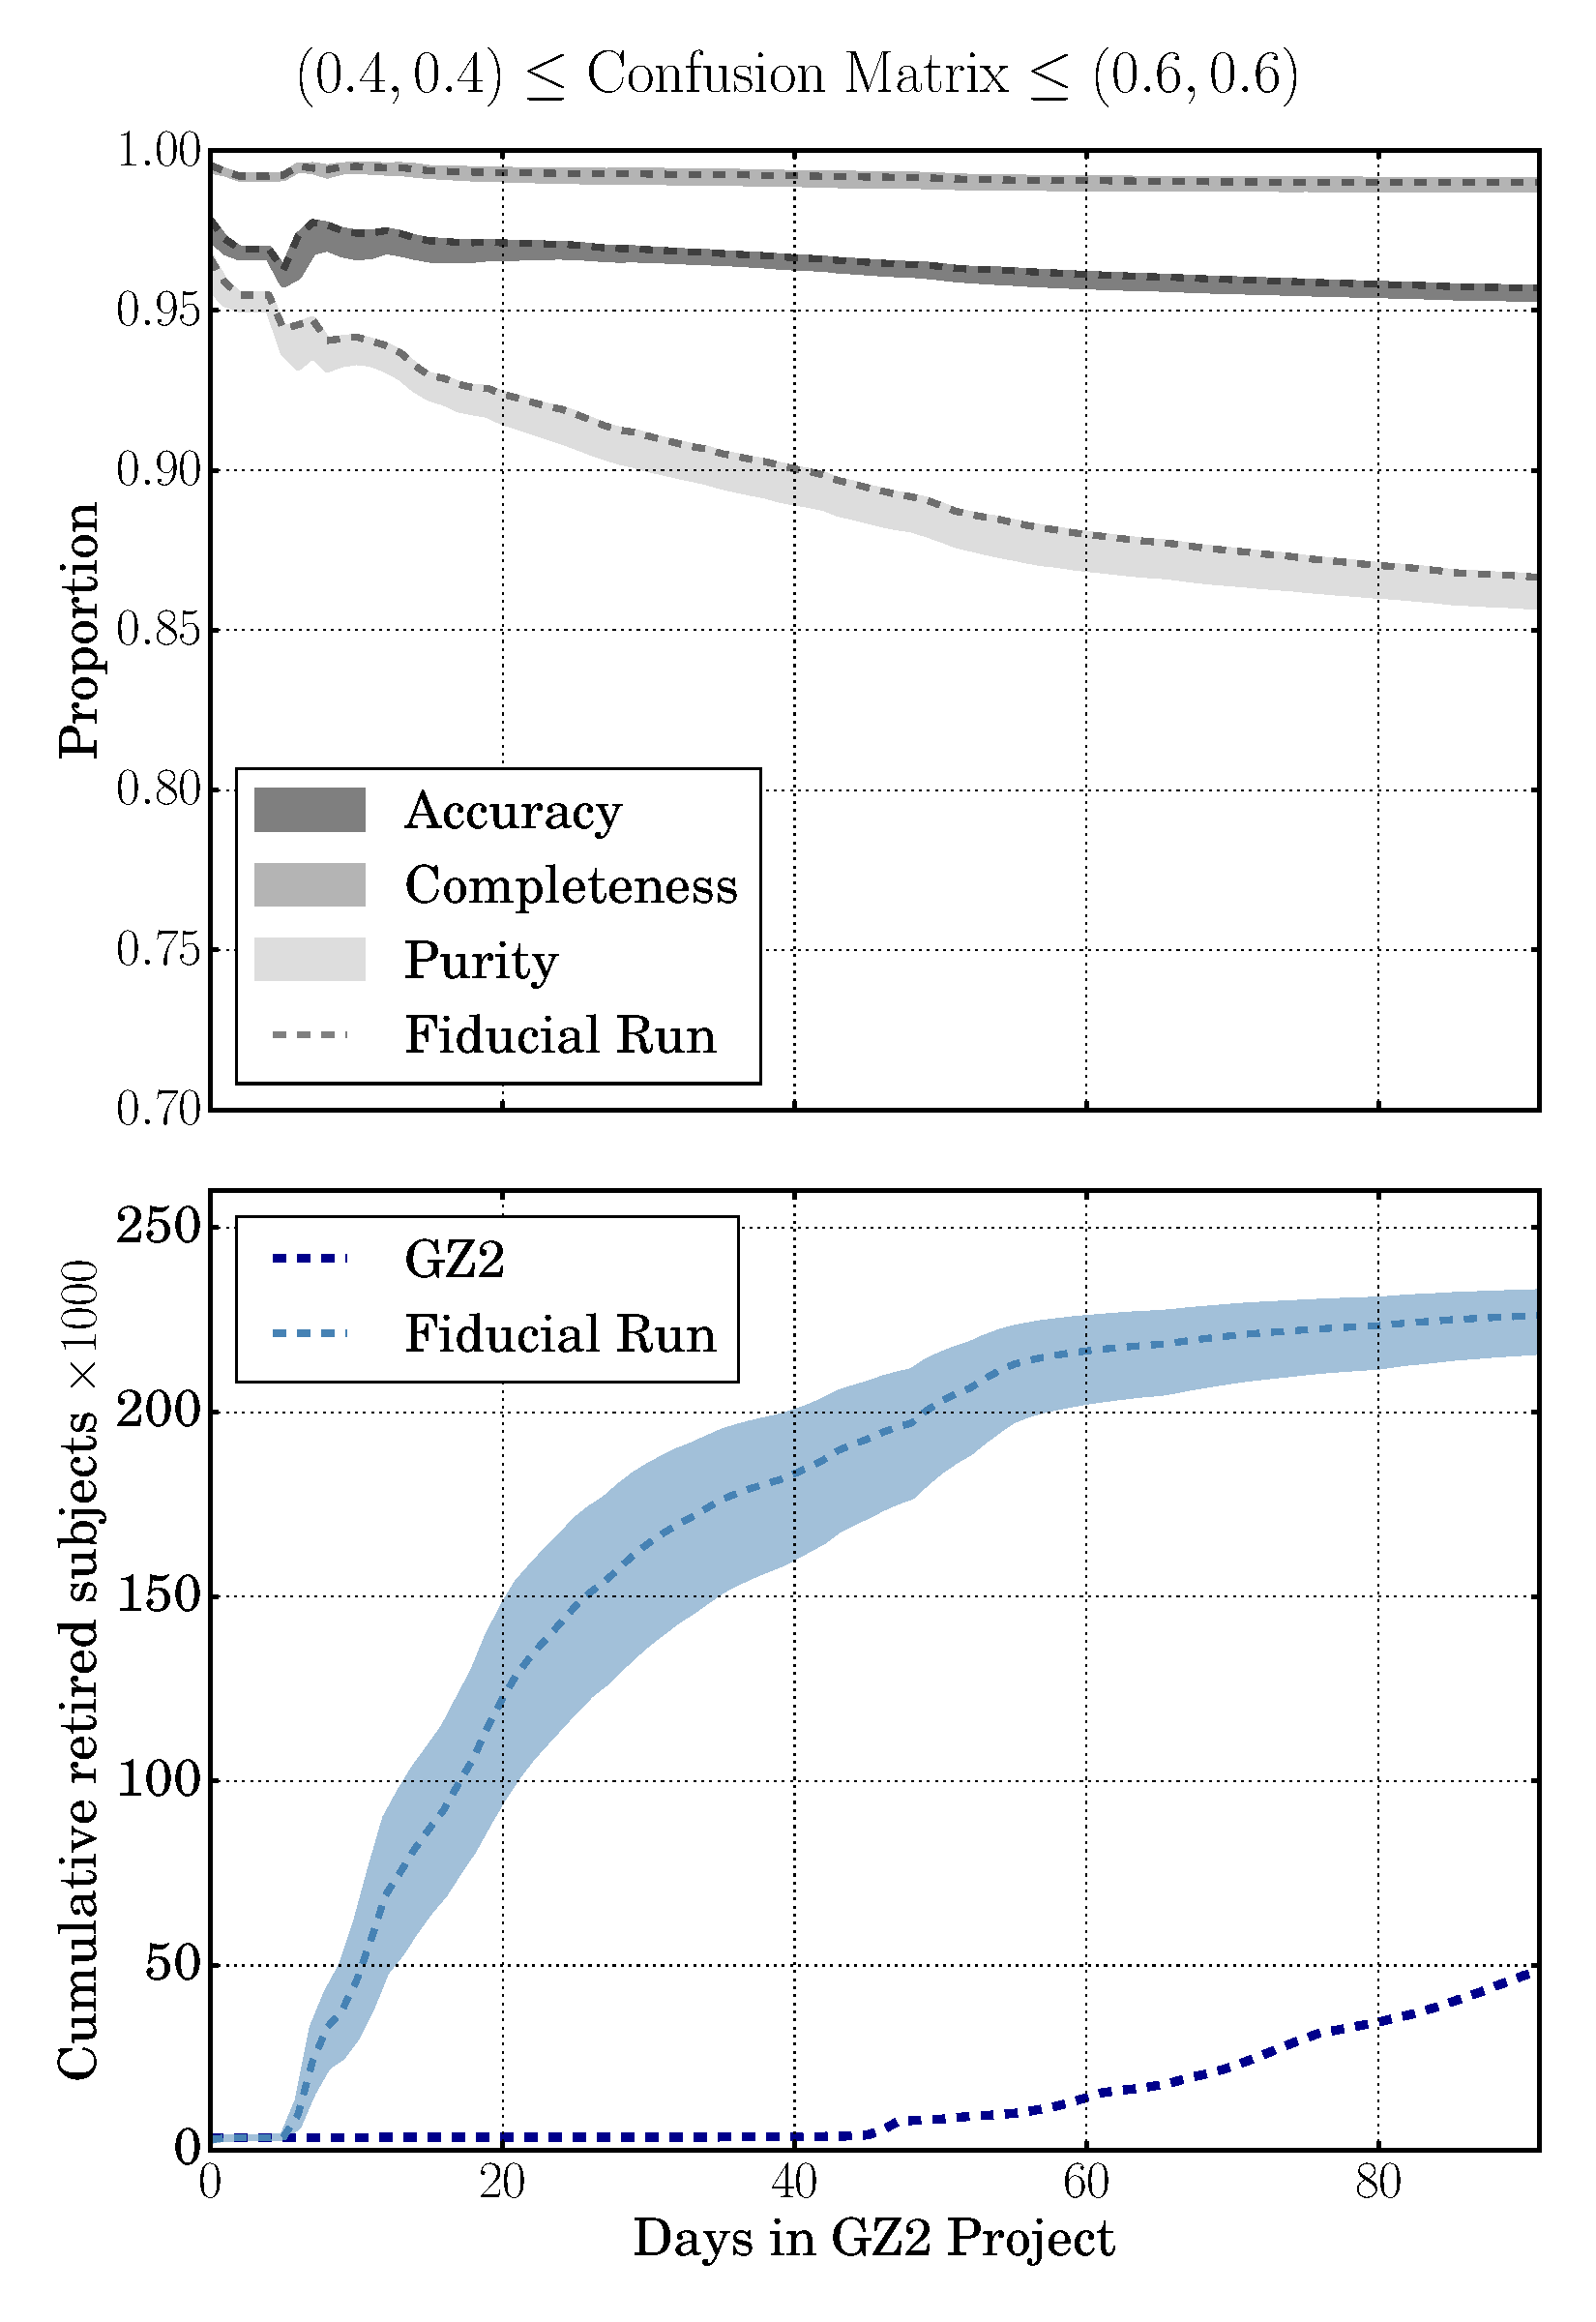
\includegraphics[width=2.8in]{Figures/human_machine/A1a.pdf}
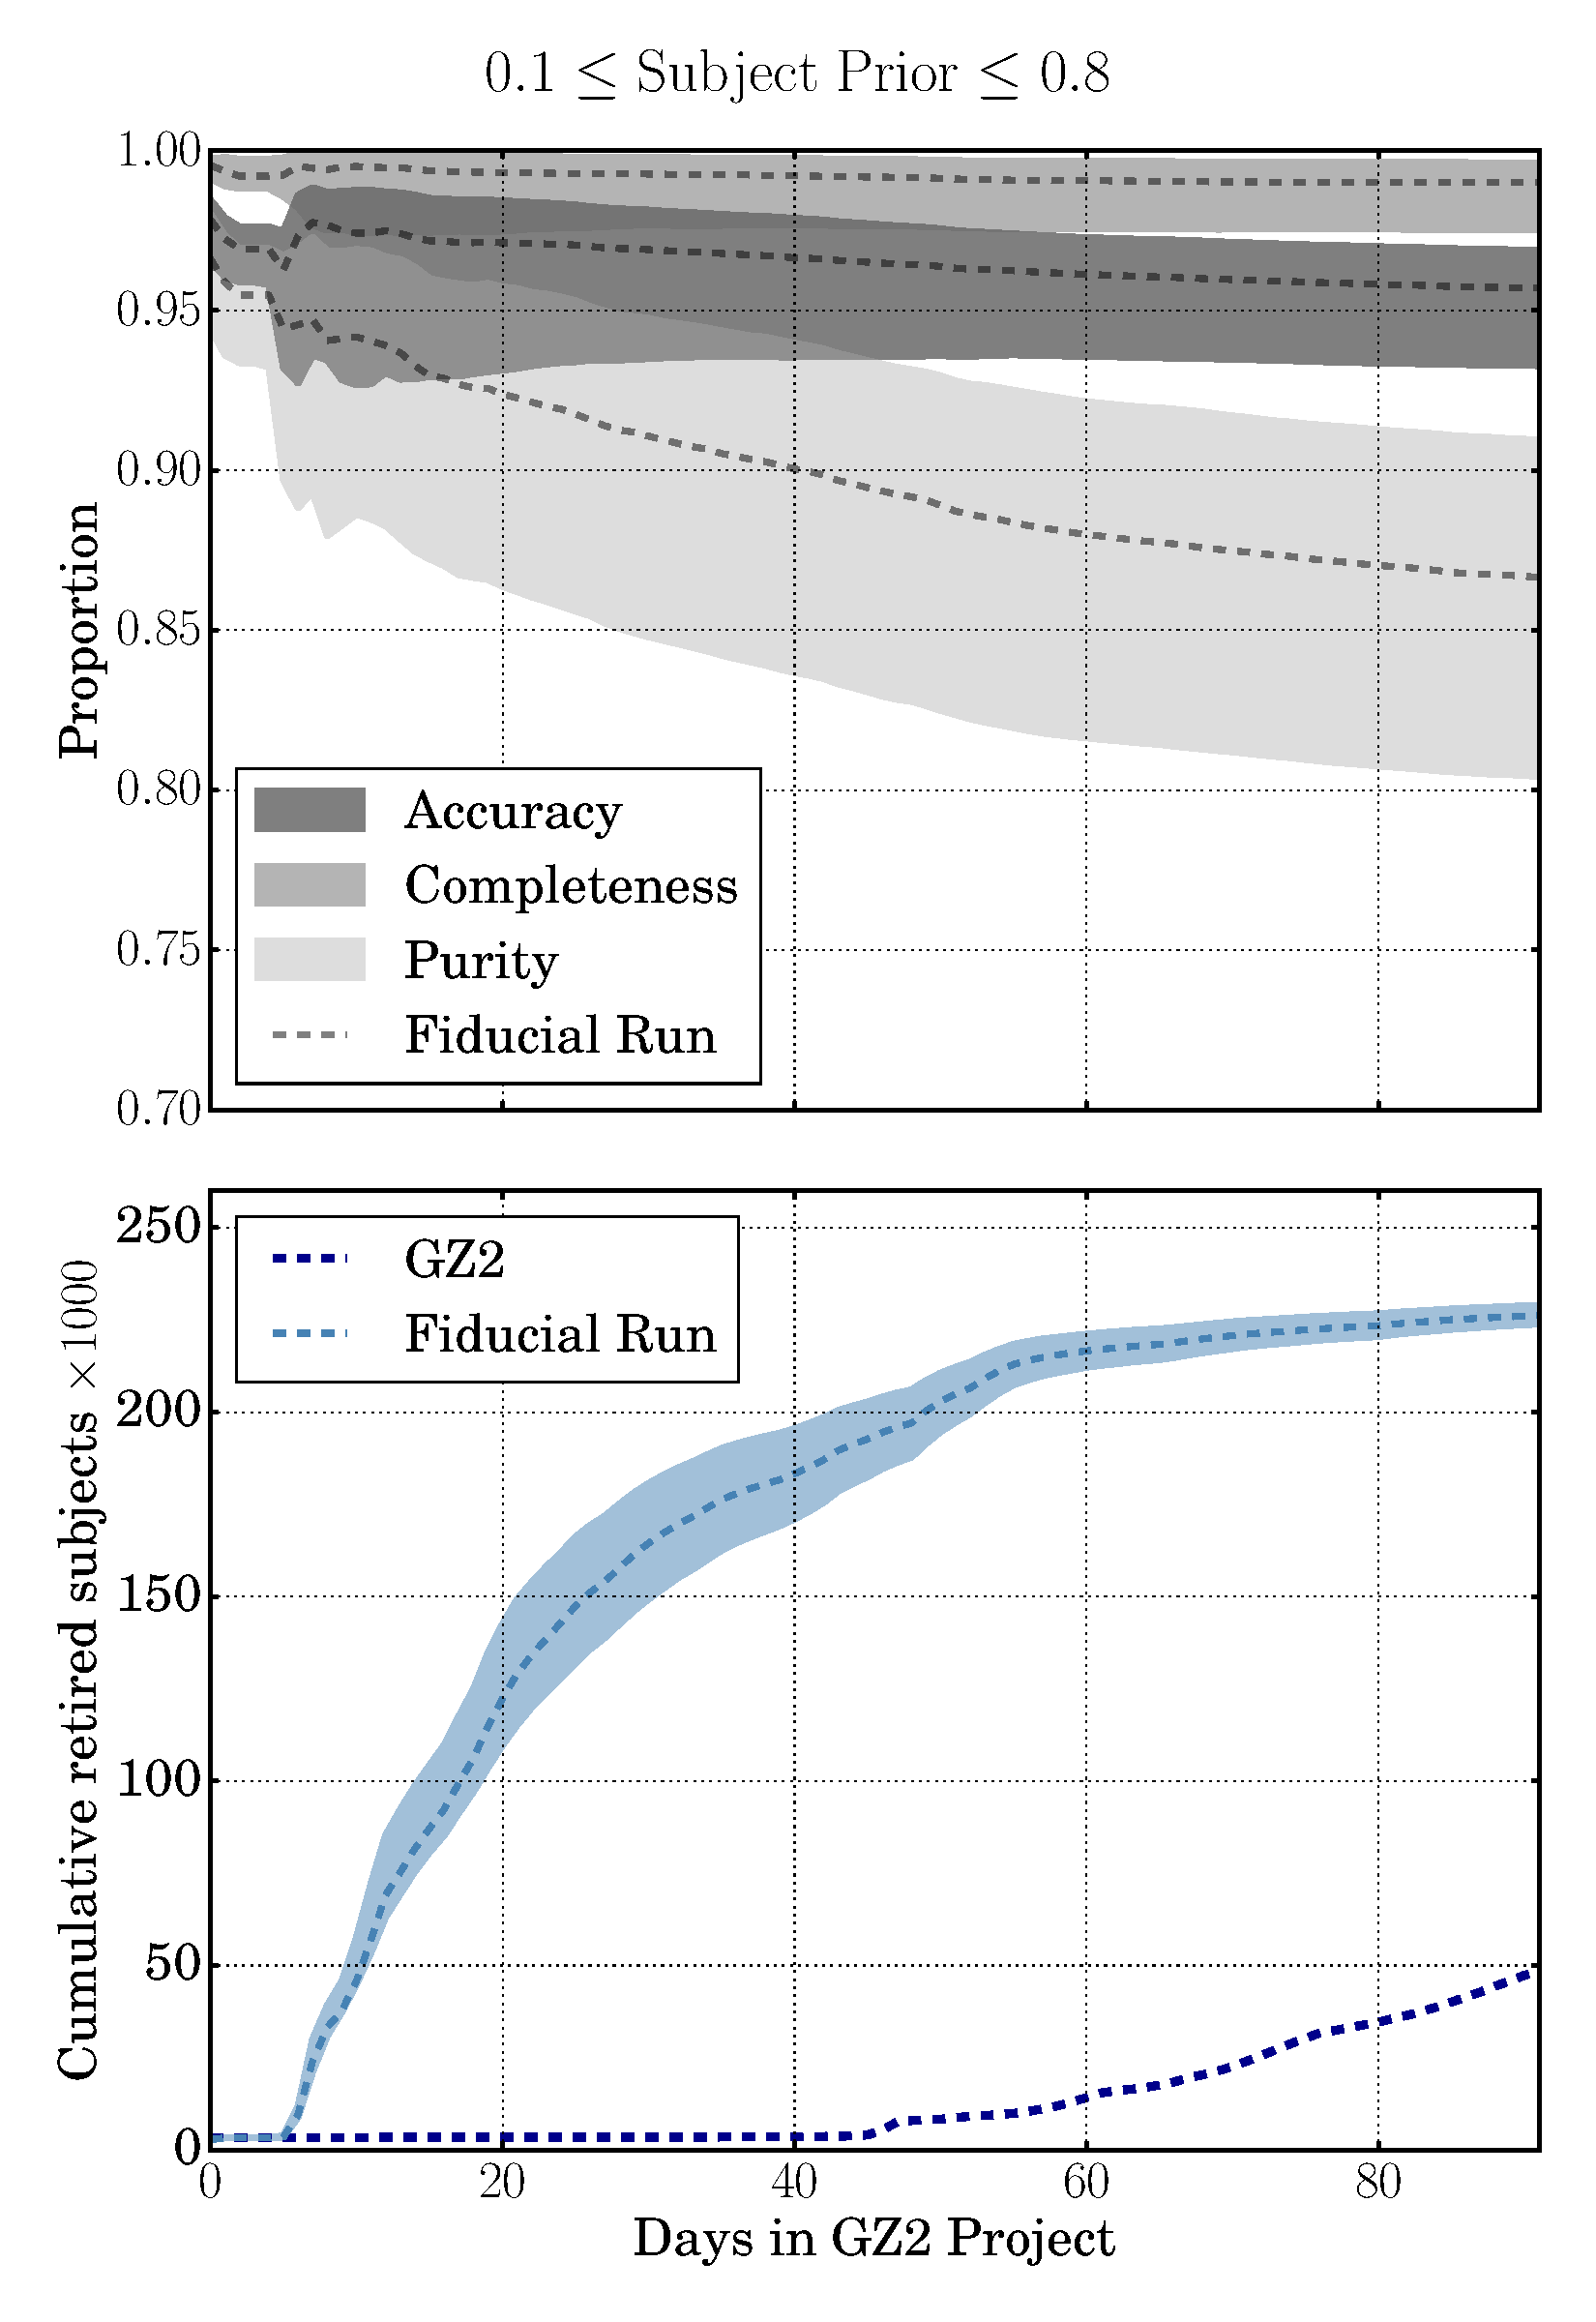
\includegraphics[width=2.8in]{Figures/human_machine/A1b.pdf}
\caption[SWAP's performance is robust to changes in initial volunteer confusion matrix and subject prior.]{SWAP performance does not dramatically change even with a range of input parameters (shaded regions) as compared to the fiducial run of Section~\ref{sec: fiducial} (dashed lines).  \textit{Left.} The quality (top) and retirement rate (bottom) when the confusion matrix is initialized as (0.4, 0.4) and (0.6, 0.6), with all other input parameters remaining constant. \textit{Right.} Same as the left panel but allowing the subject prior probability, \p $= 0.2, 0.35$ and $0.8$. Changing the confusion matrix has little impact on the quality of the labels but varies the total number of subjects retired. In contrast, changing the subject prior is more likely to affect the classification quality rather than the total number of subjects retired. \label{fig: tweak swap}}
\end{figure*}

We retire $\sim$$225$K$\pm3.5\%$ subjects as shown by the light blue shaded region in the bottom left panel of Figure~\ref{fig: tweak swap}, where the dashed blue line denotes the fiducial run. Predictably, when the confusion matrix probabilities are low, we retire fewer subjects than when these probabilities are high for a given period of time. This is easy to understand since it takes longer for volunteers to become astute classifiers when they are initially given values denoting them as obtuse. Regardless, most volunteers become astute classifiers by the end of the simulation. The top left panel demonstrates our usual quality metrics as computed in Section \ref{sec: fiducial}. The dashed lines again denote the fiducial run. We maintain $\sim$$95\%$ accuracy, $99\%$ completeness, and $\sim$$84\%$ purity;  and no metric changes by $> 2\%$ regardless of initial confusion matrix values.  
 
This spread is due to three effects: 
1) subjects can receive an alternate SWAP label in different simulations, 
2) subjects can be retired in a different order, and 
3) the set of retired subjects is not guaranteed to be common to all runs. 
We find SWAP to be highly consistent: more than 99\% of retired subjects are the same among all simulations, and, of these, 99\% receive the same label.  Instead we find that the order in which subjects are retired changes between runs. When the confusion matrix is low, subjects take longer to classify compared to the fiducial run (i.e., they retire on a later date in GZ2 project time). Likewise, subjects retire sooner when the confusion matrix is high. This can cause quality metrics to vary since they are calculated on a day to day basis. These effects each contribute less than one per cent variation and thus we see a high level of consistency between simulations. 

Of interest, perhaps, is that the quality metrics for these simulations are not symmetric about the fiducial run. However, in the Bayesian framework of SWAP, an agent with confusion matrix (0.4, 0.4) contributes as much information as an agent with confusion matrix (0.6, 0.6). The quality metrics computed are thus within a per cent of each other. In either case, we find that initializing agents at (0.5, 0.5) provides optimal performance for the `training' we simulate with our current approach. Further assessment would require a live project with real-time training and feedback. 


\subsection{Subject prior probability,~\p.}
The prior probability assigned to each subject is an educated guess of the frequency of that characteristic in the scope of the data at hand. For galaxy morphologies, this number should be an estimate of the probability of observing a desired feature (bar, disk, ring, etc.). In our case, we desire simply to find galaxies that are~\feat; however, this is dependent on mass, redshift, physical size, etc. The original GZ2 sample was selected primarily on magnitude and redshift.  As there was no cut on galaxy size (with the exception that each galaxy be larger than the SDSS PSF), the sample includes a large range of  masses and sizes. Designating a single prior is not clear-cut; we thus explore how various~\p~values effect the SWAP outcome.

We run simulations allowing~\p~to take values 0.2, 0.35, and 0.8 
and compare these to the fiducial run, with everything else remaining constant. The results are shown in the right panels of Figure~\ref{fig: tweak swap}. We again find that SWAP is consistent in terms of subject retirement which varies by only 1\%. However, as can be seen in the top panel, the variation in our quality metrics is more pronounced. Firstly, though we retire nearly the same number of subjects over the course of each simulation, they are less consistent than our previous runs. That is, only 95\% of retired subjects are common to all simulations. Secondly, of those that are common, only 94\% receive the same label from SWAP indicating that hanging the prior is more likely to produce a different label for a given subject than changing the initial agent confusion matrix. Finally, there is also a larger spread for the day on which a subject is retired as compared to the fiducial run. These trends all contribute to a broader spread in accuracy, completeness, and purity as a function of project time. We stress, however, that although more substantial than the previous comparison, these variations are all within $\pm5\%$. 

We can understand these variations more intuitively by considering the following. Recall that our retirement thresholds,~\tf~and~\tn, have not changed in these simulations. When~\p~is small, the subject's probability is already closer to~\tn~in probability space, and thus more subjects are classified as~\notfeat~compared to the fiducial run. Similarly, when~\p~is large, some of these same subjects can instead be classified as~\feat~because~\p~is already closer to~\tf. Obviously, both outcomes cannot be correct. We find that the simulation with~\p~= 0.8 performs the worst of any run; this is a direct reflection of the fact that this prior is not suitable for this question or this dataset. Indeed, the best performance is achieved when~\p = 0.35.  This reflects the distribution of~\feat~subjects as determined by~\raw~labels and is more characteristic of the expected proportion of~\feat~galaxies in the local universe. As a value far from the correct value can have a significant impact on the classification quality, it is important to choose a prior wisely.


%%%-------------------------------------------------------
%%%  FIGURE:   SWAP THRESHOLDS
%%%-------------------------------------------------------
\begin{figure}
\begin{center}
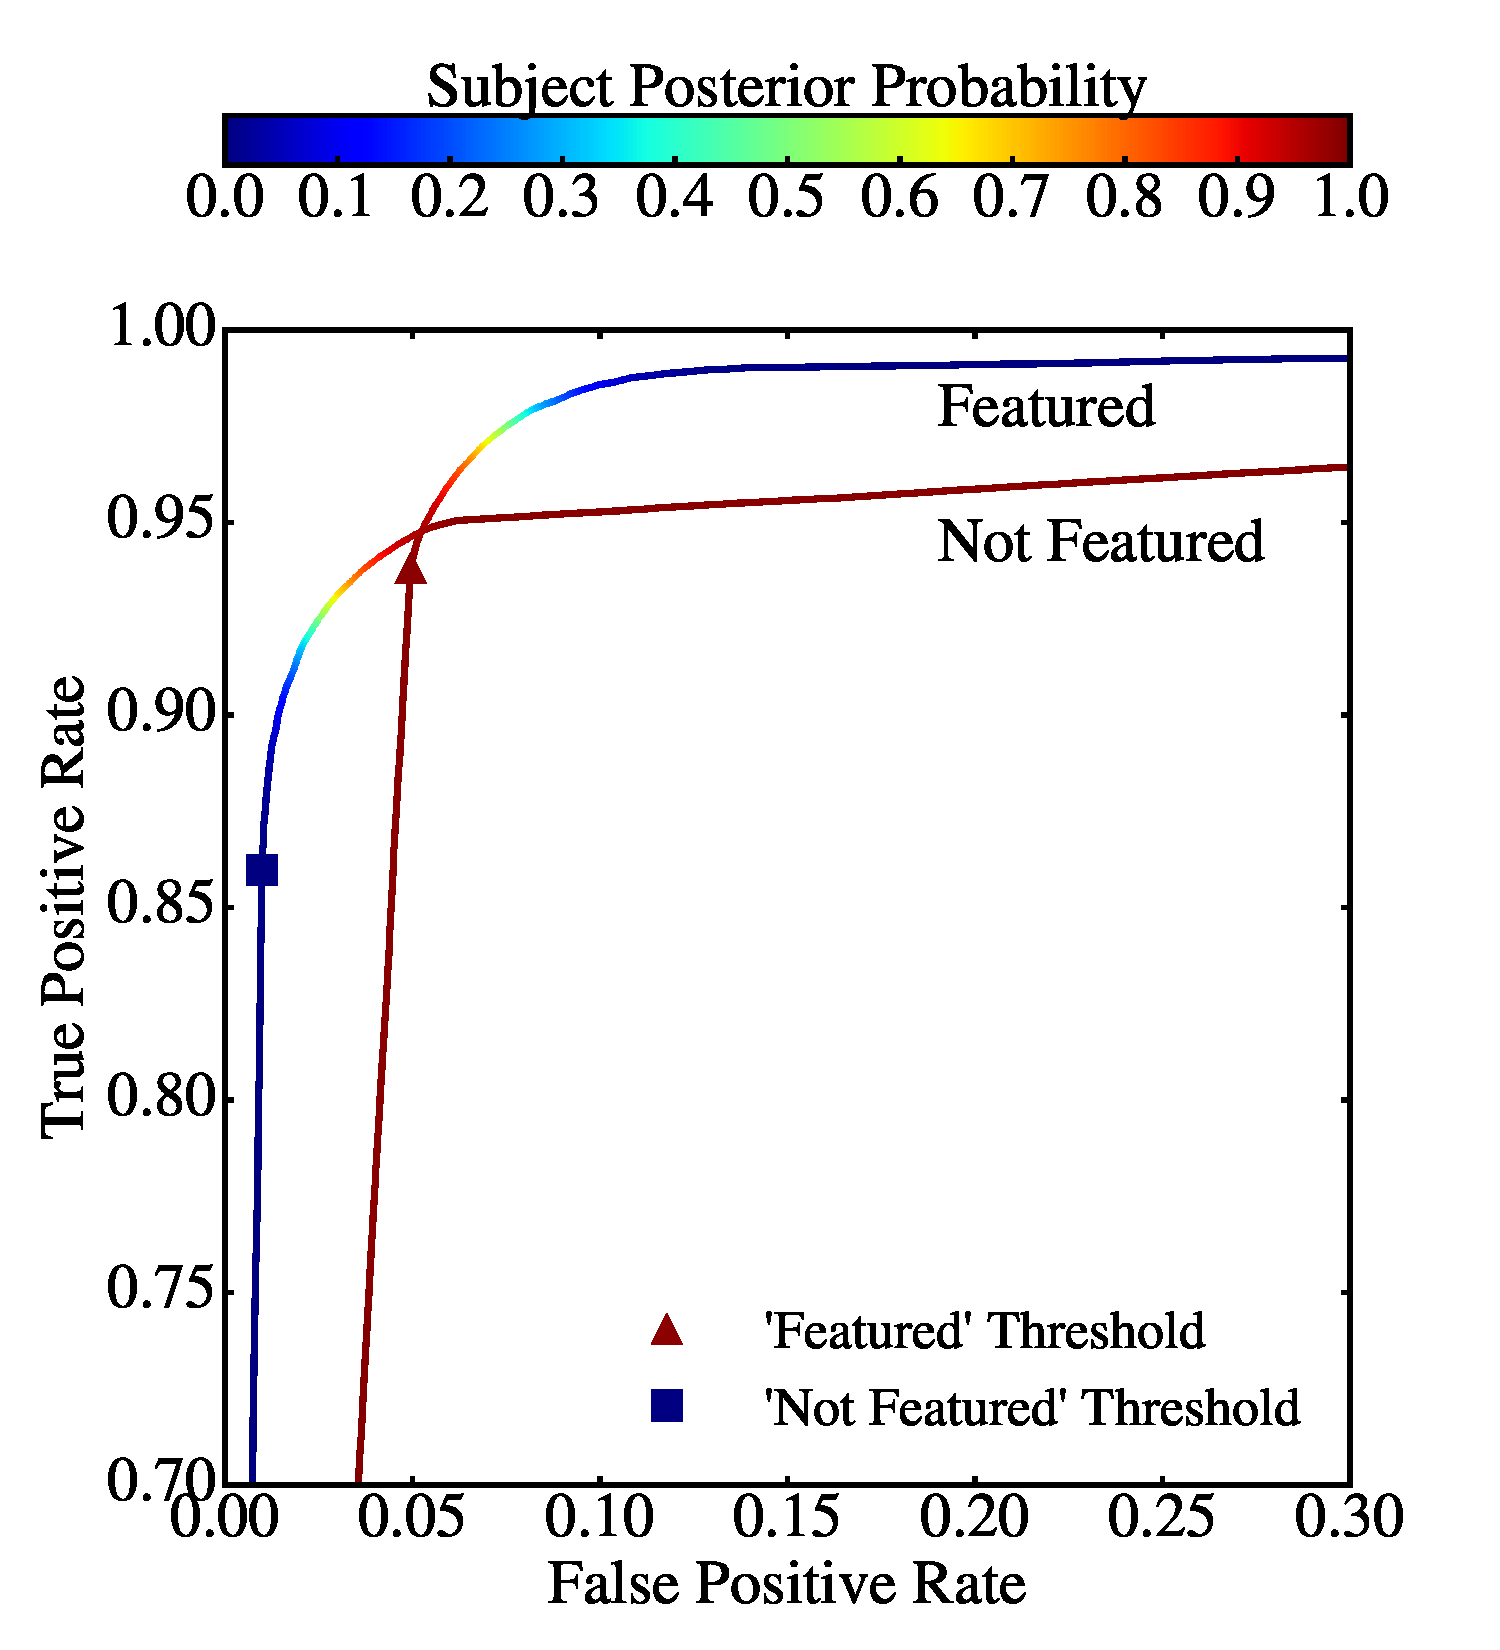
\includegraphics[width=3.08in]{Figures/human_machine/A2a.pdf}
\caption[Receivor operating characteristic curve for the chosen SWAP retirement thresholds.]{Identifying~\feat~subjects is independent of identifying~\notfeat~subjects.  Both ROC curves use all subjects processed by SWAP where the score used to create the ROC curve is simply each subject's achieved posterior probability. The Featured curve demonstrates how well we identify~\feat~subjects with a threshold of 0.99, while the Not Featured curve demonstrates how well we identify~\notfeat~subjects with a threshold of 0.004. Typically, best performance is achieved by the score associated with the upper-left-most part of the curve. Our~\feat~threshold is nearly optimal, while our~\notfeat~threshold could be improved since the blue square is not as close to the upper left hand corner as other possible values of the subject posterior.}
\label{fig: morph thresh}
\end{center}
\end{figure}

\subsection{Retirement thresholds, \tf~and~\tn.}
Retirement thresholds are directly related to the time that a subject will spend in SWAP before retirement. If we lower~\tf~(and/or raise~\tn), more subjects will be retired compared to the fiducial run as each subject will have a smaller swath of probability space in which to fluctuate before crossing one of these thresholds. On the other hand, if we raise~\tf~(and/or lower~\tn), it will take longer for subjects to cross one of these thresholds. This also increases the likelihood of some subjects never crossing either threshold, instead oscillating indefinitely through probability space.

What thresholds should one choose? To answer this question, we consider the left panel of Figure~\ref{fig: morph thresh}, which depicts the receiver operating characteristic (ROC) curve for our fiducial simulation, an illustration of performance as a function of a threshold for a binary classifier. ROC curves display the true positive rate against the false positive rate for a discriminatory threshold or score with a perfect classifier achieving 100\% true positives and no false positives. The value of the threshold optimal for predicting class labels would be that which allows the ROC curve to reach the upper-left-most point in the diagram. We have two thresholds to consider and thus we plot the curve twice: once under the assumption that ``true positives" denote correctly identified~\feat~subjects; and again under the assumption that ``true positives" instead denote correctly identified~\notfeat~subjects.  In both cases, the color of the line corresponds to the subject posterior probability. We mark the location of~\tf~$=0.99$~and~\tn~$=0.004$
from our fiducial run with a red triangle and blue square respectively. We see that~\tf~is nearly optimal but~\tn~could be improved upon. 
%!TEX root = thesis.tex

\chapter{Incorporating machine intelligence}
\label{chap:4}



%%----------------------------------------------------------------------------------------------------------------------------------------------------
%%   INTEGRATING MACHINE CLASSIFIERS 
%%----------------------------------------------------------------------------------------------------------------------------------------------------
\section{Efficiency through incorporation of machine classifiers} \label{sec: machine}

We construct the full Galaxy Zoo Express by incorporating supervised 
learning, the machine learning task of inference from labelled training data. 
The training data consist of a set of training examples, and must include
an input feature vector and a desired output label.  Generally speaking,
a supervised learning algorithm analyses the training data and produces a 
function that can be mapped to new examples. A properly optimized algorithm will 
correctly determine class labels for unseen data. By processing human classifications 
through SWAP, we obtain a set of binary labels by which we can train a machine 
classifier. We briefly outline the technical details of our machine below,  turning
towards the decision engine we develop in Section~\ref{sec: decision engine}. 



%%----------------------------------------------------------------------------------------------------------------------------------------------------
%%   RANDOM FORESTS
%%----------------------------------------------------------------------------------------------------------------------------------------------------
\subsection{Random Forests}
We use a Random Forest (RF) algorithm~\citep{Breiman2001},  
an ensemble classifier that operates by
 bootstrapping the training data and constructing a multitude of individual decision 
tree algorithms, one for each subsample.  
An individual decision tree works by deciding which of 
the input features best separates the classes. It does this by performing 
splits on the values of the input feature that minimize the classification 
error. These feature splits proceed recursively. Decision trees alone are
 prone to over-fitting, precluding them from generalizing 
well to new data. Random Forests mitigate this effect by combining the 
output labels from a multitude of decision trees.  Specifically, we use the 
\texttt{RandomForestClassifier} from the Python module \texttt{scikit-learn}
\citep{scikit-learn}. 


%%----------------------------------------------------------------------------------------------------------------------------------------------------
%%   CROSS-VALIDATION
%%----------------------------------------------------------------------------------------------------------------------------------------------------
\subsection{Grid Search and Cross-validation}
Of fundamental importance is the task of choosing an algorithm's hyperparameters, 
values which determine how the machine learns.   For a RF, key quantities include
 the maximum depth of individual trees (\texttt{max\_depth}), the number of trees
in the forest (\texttt{n\_estimators}), and the number of features to consider when 
looking for the best split (\texttt{max\_features}). 
The goal is to determine which values will optimize 
the machine's performance and thus these values cannot be chosen \textit{a priori}. 
We perform a grid search with $k$-fold cross-validation whereby the 
training sample is split into $k$ subsamples. One subsample is withheld to 
estimate the machine's performance while the remaining data are used to train the machine. 
This is performed $k$ times and the average performance
value is recorded. The entire process is repeated for every combination of the 
 hyperparameters in the grid space and values that optimize the output are chosen. 
In this work we let $k=10$, however, we leave this as an adjustable input parameter.
In the interest of computational speed, we set \texttt{n\_estimators} $=30$ and 
perform the grid search for \texttt{max\_depth} over the range $[5,16]$, and 
\texttt{max\_features} over the range $[\sqrt{D}, D]$,
where $D$ is the number of features in the feature vector, described below.
 

%%----------------------------------------------------------------------------------------------------------------------------------------------------
%%   FEATURE REPRESENTATION AND PRE-PROCESSING
%%----------------------------------------------------------------------------------------------------------------------------------------------------
\subsection{Feature Representation and Pre-Processing}
The feature vector on which the machine learns is composed of $D$ individual 
numeric quantities associated with the subject that the machine uses to discern 
that subject from others in the training sample. 
To segregate~\feat~from~\notfeat, we draw on ZEST \citep{Scarlata2007} and compute
 concentration, asymmetry, Gini coefficient, and M$_{20}$, 
the second-order moment of light for the brightest 20\% of galaxy pixels as
measured from SDSS DR12 $i$-band imaging (see Appendix \ref{sec: measuring morphology}). 
Coupled with SExtractor's measurement of ellipticity \citep{sextractor}, 
we provide the machine with a $D=5$ dimensional morphology parameter space.
These non-parametric diagnostics have long been used to distinguish between early- and late-type galaxies 
in an automated fashion \cite[e.g.,][]{Abraham1996, Bershady2000, Conselice2000, Abraham2003, Conselice2003, Lotz2004, Snyder2015}.
Because the RF algorithm handles a variety of input formats, the only pre-processing 
step we perform is the removal of poorly-measured morphological indicators, i.e. catastrophic failures.



%%%-------------------------------------------------------
%%%  FIGURE:   LEARNING CURVE
%%%-------------------------------------------------------
\begin{figure}[t!]
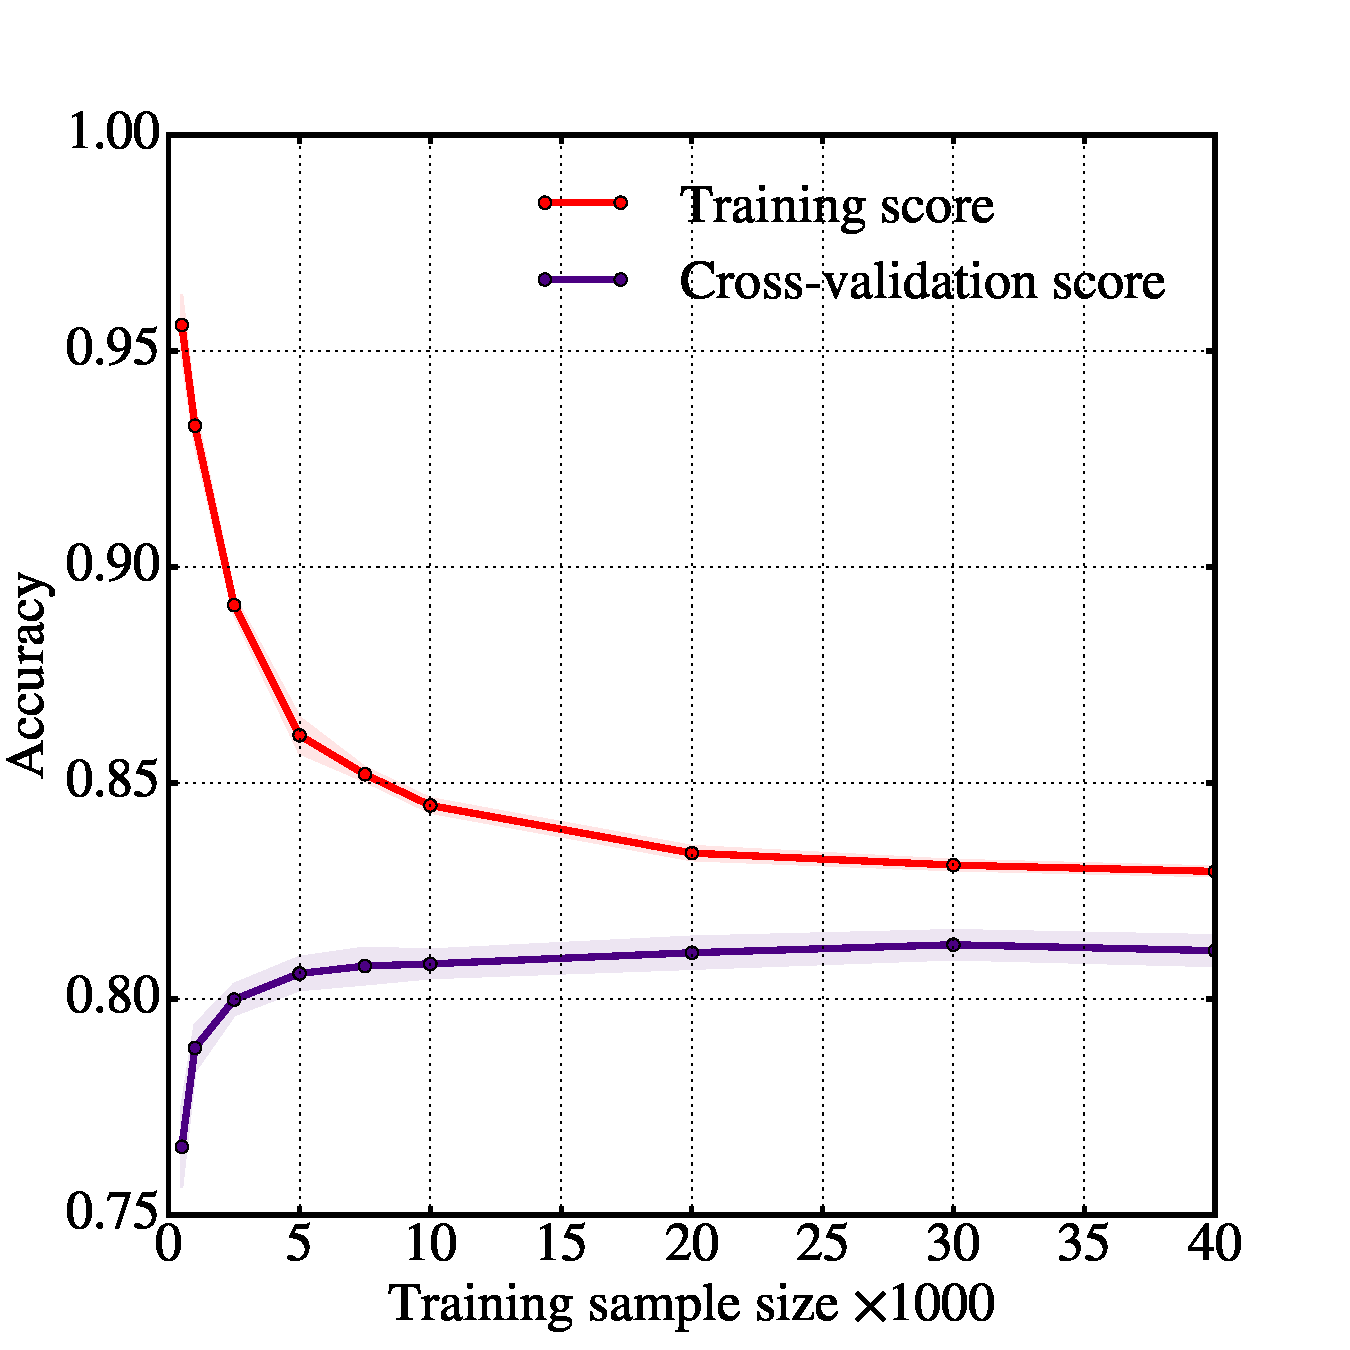
\includegraphics[width=3.25in]{Figures/human_machine/f6.pdf}
\caption[Random Forest learning curve]{Learning curve for a Random Forest with fixed hyperparameters. These curves show the mean accuracy computed during cross-validation and on the training sample, where the shaded regions denote the standard deviation. When the training sample size is small, the machine accurately identifies its own training sample but is unable to generalize to unseen data as evidenced by a low cross-validation score. As the training sample size increases, the cross-validation score increases. This behaviour plateaus indicating that larger training samples provide little in additional performance. \label{fig: learning curve}}
\end{figure}


%%----------------------------------------------------------------------------------------------------------------------------------------------------
%%   DECISION ENGINE 
%%----------------------------------------------------------------------------------------------------------------------------------------------------
\subsection{Decision Engine}\label{sec: decision engine}
A number of decisions must be addressed before attempting to train the machine. 
In particular, which subjects should be designated as the training sample? 
When should the machine attempt its first training session? 
When has the machine's performance been optimized such that it will successfully
generalize to unseen subjects? The field of machine learning provides few hard rules 
for answering these questions, only guidelines and best practices. 
Here we briefly discuss our approach for the development of our decision engine.

%%%-------------------------------------------------------
%%%  FIGURE:    FULL GZX PERFORMANCE
%%%-------------------------------------------------------
\begin{figure*}[t!]
\centering
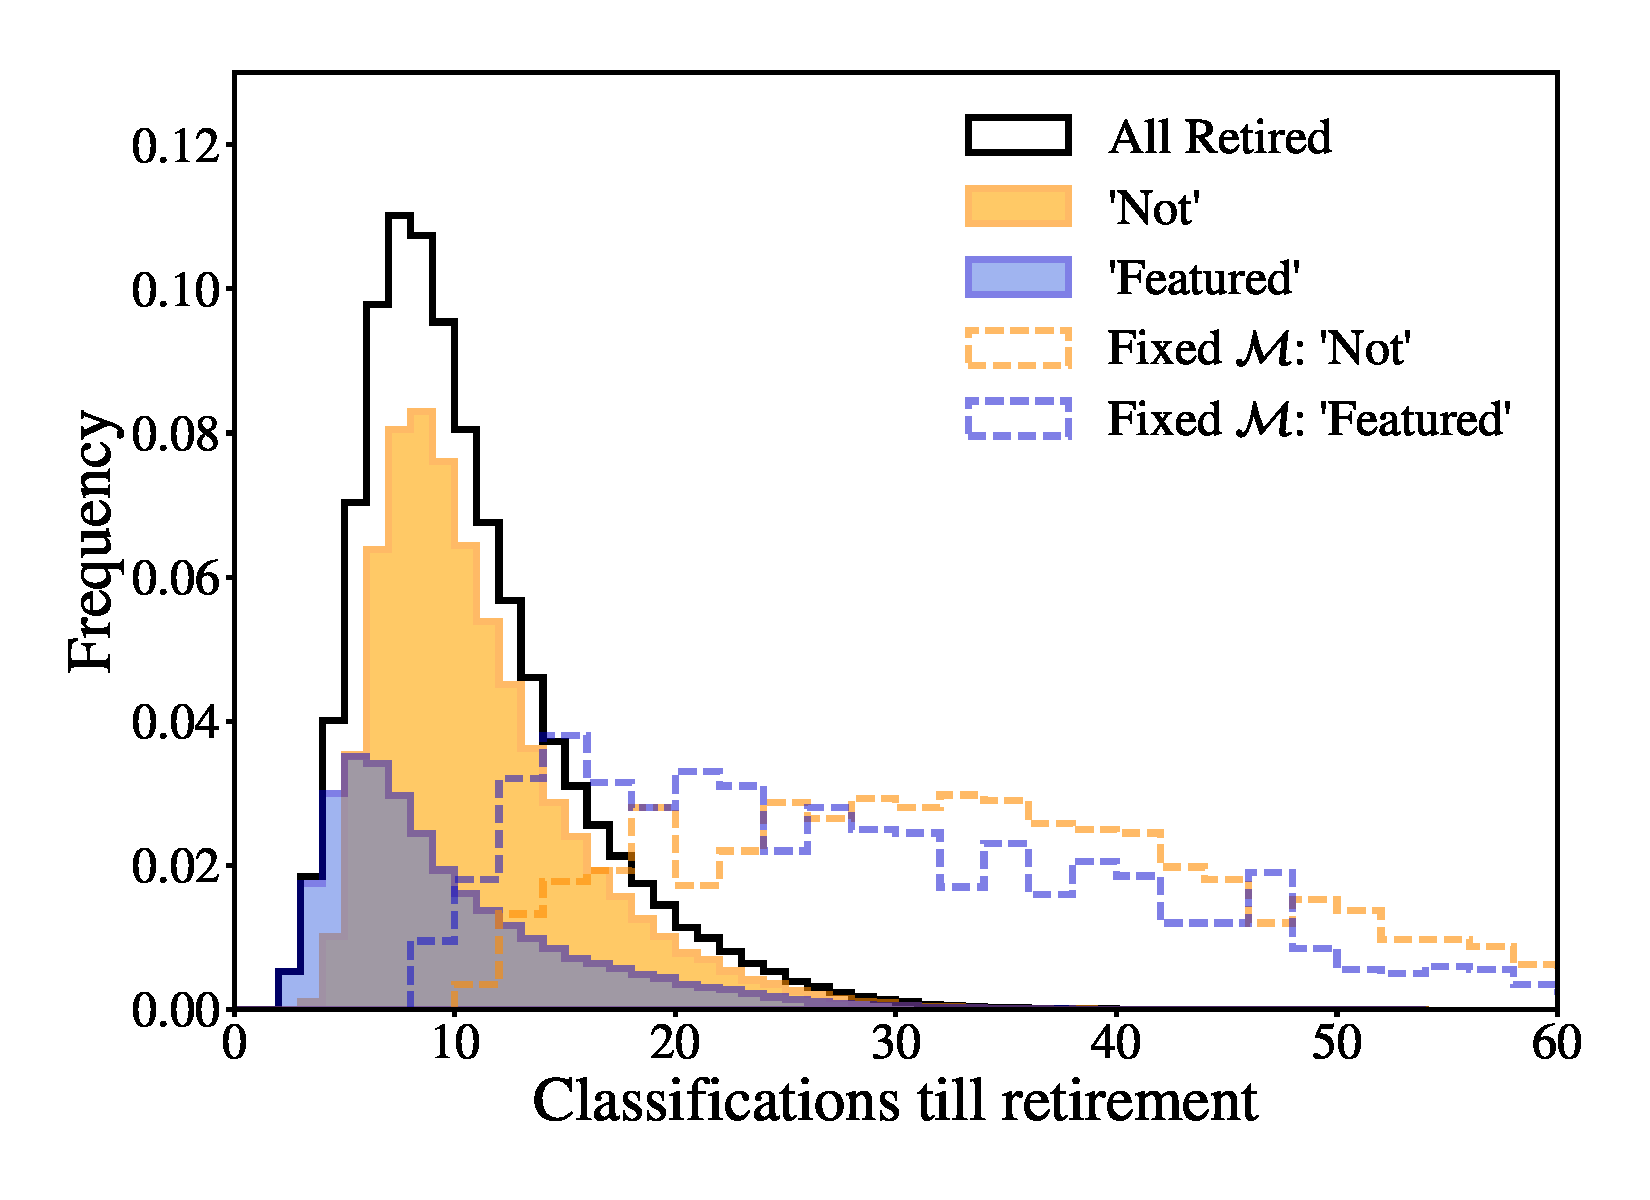
\includegraphics[width=5.5in]{Figures/human_machine/f7.pdf}
\caption[Performance of the human+machine combination -- Galaxy Zoo: Express]{By incorporating a machine classifier, GZX (red) increases the classification rate by an order of magnitude compared to GZ2 (dashed dark blue) and out-performs the SWAP-only run (light blue), retiring more than 200K subjects in just 27 days of GZ2 project time. The dashed black line marks the first night the machine trains. After several additional nights of training, it is deemed optimized and allowed to retire subjects. Both humans and machine then contribute to retirement. We end the simulation after 32 days having retired over 210K galaxies. See Table~\ref{tab: summary} for details. \label{fig: money}}
\end{figure*}


As discussed in detail in Section~\ref{sec: SWAP}, SWAP yields a probability that 
a subject exhibits the feature of interest. While some machine algorithms can 
accept continuous input labels, the RF requires distinct classes. We thus use only 
those subjects which have crossed either of the retirement thresholds. 
Though we find that SWAP consistently retires 35-40\%~\feat~subjects on 
any given day of the simulation, a balanced ratio of~\feat~to~\notfeat~isn't guaranteed.
 Highly unbalanced training samples should be resampled to correct the imbalance; 
however, as we exhibit only a mild lopsidedness, we allow the machine to train on all 
SWAP-retired subjects.  

SWAP retires a few hundred subjects during the first days of the simulation.
In principle,  a machine can be trained with such a small sample, but will be unable
to generalize to unseen data. We estimate a minimum number of training samples
and the machine's ability to generalize by considering a learning curve, an illustration
of a machine's performance with increasing sample size for fixed hyperparameters. 
Figure~\ref{fig: learning curve} demonstrates such a curve wherein we plot
the accuracy from both the 10-fold cross-validation, and the trained machine
applied to its own training sample for a random sample of GZ2 subjects
required to be balanced between~\feat~and~\notfeat.  
We fix the RF's hyperparameters as follows: \texttt{max\_depth} $=8$, 
\texttt{n\_estimators } $=30$, and \texttt{max\_features} $=2$. 
When the sample size is small, the cross-validation score is low and the training 
score is high, a clear sign of over-fitting.  However, as the training 
sample size increases, the cross-validation score increases and eventually plateaus,
 indicating that larger training sets will yield little additional gain. 

We estimate this plateau begins when the training 
sample reaches 10,000 subjects and require SWAP retire at least this many 
 before the machine attempts its first training.  We estimate the machine 
has trained sufficiently if the cross-validation score fluctuates by less than 1\% 
for three consecutive nights of training to ensure we have reached the plateau.  
This requires that we record the machine's training performance each night, 
including how well it scores on the training sample, the 
cross-validation score, and the best hyperparameters. 



%%----------------------------------------------------------------------------------------------------------------------------------------------------
%%   MACHINE SHOP 
%%----------------------------------------------------------------------------------------------------------------------------------------------------
\subsection{The Machine Shop}\label{sec: machine shop}
We can now describe a full GZX simulation, which begins with human classifications 
processed through SWAP for several days.   
Once at least 10K subjects have been retired, their feature vectors are passed to 
the machine for its inaugural training. 
A suite of performance metrics are recorded by a machine agent, similar
in construction to SWAP's agents. This agent determines 
when the machine has trained sufficiently by assessing the variation
in performance metrics for all previous nights of training. 
Once the machine has been optimized, the agent introduces it to the test sample
consisting of any subject that has not yet reached retirement through SWAP 
and is not part of the gold standard sample.  

Analogous to SWAP, we generate a retirement rule for machine-classified subjects. 
In addition to the class prediction, the RF algorithm computes the probability for
each subject to belong to each class.  This probability is simply the average of
 the probabilities of each individual decision tree, where the probability of a 
single tree is determined as the fraction of subjects of class X on a leaf node.  
Only subjects that receive a class prediction of \feat with 
$p_{\mathrm{machine}} \ge 0.9$ ($p_{\mathrm{machine}} \le 0.1$ for \notfeat)
are considered retired. 
The remaining subjects have the possibility of being classified by humans 
or the machine on a future night of the simulation. 
This constitutes the core of our passive feedback mechanism. Subjects that are
not retired by the machine can instead be retired by humans, thus providing 
the machine a more fully sampled morphology parameter space on future 
training sessions. 




%%----------------------------------------------------------------------------------------------------------------------------------------------
%%   RESULTS 
%%----------------------------------------------------------------------------------------------------------------------------------------------
\section{Results} \label{sec: results}
We perform a full GZX simulation incorporating our RF with the fiducial 
SWAP run discussed in Section~\ref{sec: fiducial}. 
The machine attempts its first training on Day 8 with an initial training
sample of $\sim$20K subjects. It undergoes several additional nights 
of training, each time with a larger training sample. 
By Day 12, SWAP has provided over 40K subjects for training and the machine's 
agent has deemed the machine optimized. 
The machine predicts class labels for the remaining 230K GZ2 subjects. 
Of those, the machine retires over 70K, dramatically increasing the 
subset of retired subjects. 
We end the simulation after 32 days, having retired $\sim$210K subjects
as detailed in Table~\ref{tab: summary}. 

We present these results in Figure~\ref{fig: money} where subject retirement 
with GZX (red) is compared to our fiducial SWAP-only run (light blue) and GZ2 (dashed dark blue). 
Using the~\raw~labels as before, we compute our usual quality metrics on the 
full sample of GZX-retired subjects; reported in Table~\ref{tab: summary}. 
Accuracy and purity remain within a few percent of the SWAP-only run at 93.5\% 
and 84.2\% respectively. Instead we see a 5\% decline in the completeness. 
While the SWAP-only run identified 99\% of~\feat~subjects, incorporation
of the machine seems to miss a significant portion thus dropping GZX completeness to 94.3\%. 
We discuss this behaviour below.

By dynamically generating a training sample through a more sophisticated analysis of 
human classifications coupled with a machine classifier, we retire more than 200K 
GZ2 subjects in just 27 days.  Visual classification through SWAP alone retires as 
many in 50 days, while GZ2 requires a full year.  
Though our analysis considers only the top-level task of GZ2's decision tree, GZX suggests a tantalizing potential to increase the classification rate by an order of magnitude over the traditional crowd-sourced approach.
We next explore the composition of those classifications.



%%----------------------------------------------------------------------------------------------------------------------------------------------
%%   WHO RETIRES WHAT, WHEN? 
%%----------------------------------------------------------------------------------------------------------------------------------------------
\subsection{Who retires what, when?}  

In the top panel of Figure~\ref{fig: gzx components} we explore the individual 
contributions to GZX subject retirement from the RF (dash-dotted teal) 
and SWAP (dashed orange). The solid black line shows the total GZX retirement (SWAP+RF), while the dotted grey line depicts the fiducial SWAP-only run from 
Section~\ref{sec: fiducial} for reference. 
Two things are immediately obvious. First, each component shoulders approximately
half of the retirement burden with the machine and SWAP responsible for 
$\sim$$100$K and $\sim$$110$K subjects respectively.  
Secondly, the rate of retirement exhibited by the two components is in stark contrast.
SWAP retires at a relatively constant rate while the machine retires 
dramatically at the beginning of its application, quickly surpassing the human 
contribution, and plateaus thereafter. 
We thus clearly see three epochs of subject retirement.
In the first phase, humans are the only contributors to subject retirement.  
Once the machine is optimized, it immediately contributes more to retirement than humans.
However, the machine's performance plateaus quickly;  the third 
phase is again dominated by human classifications.

%%%-------------------------------------------------------
%%%  FIGURE:    GZX COMPONENT CONTRIBUTIONS
%%%-------------------------------------------------------
\begin{figure}[t!]
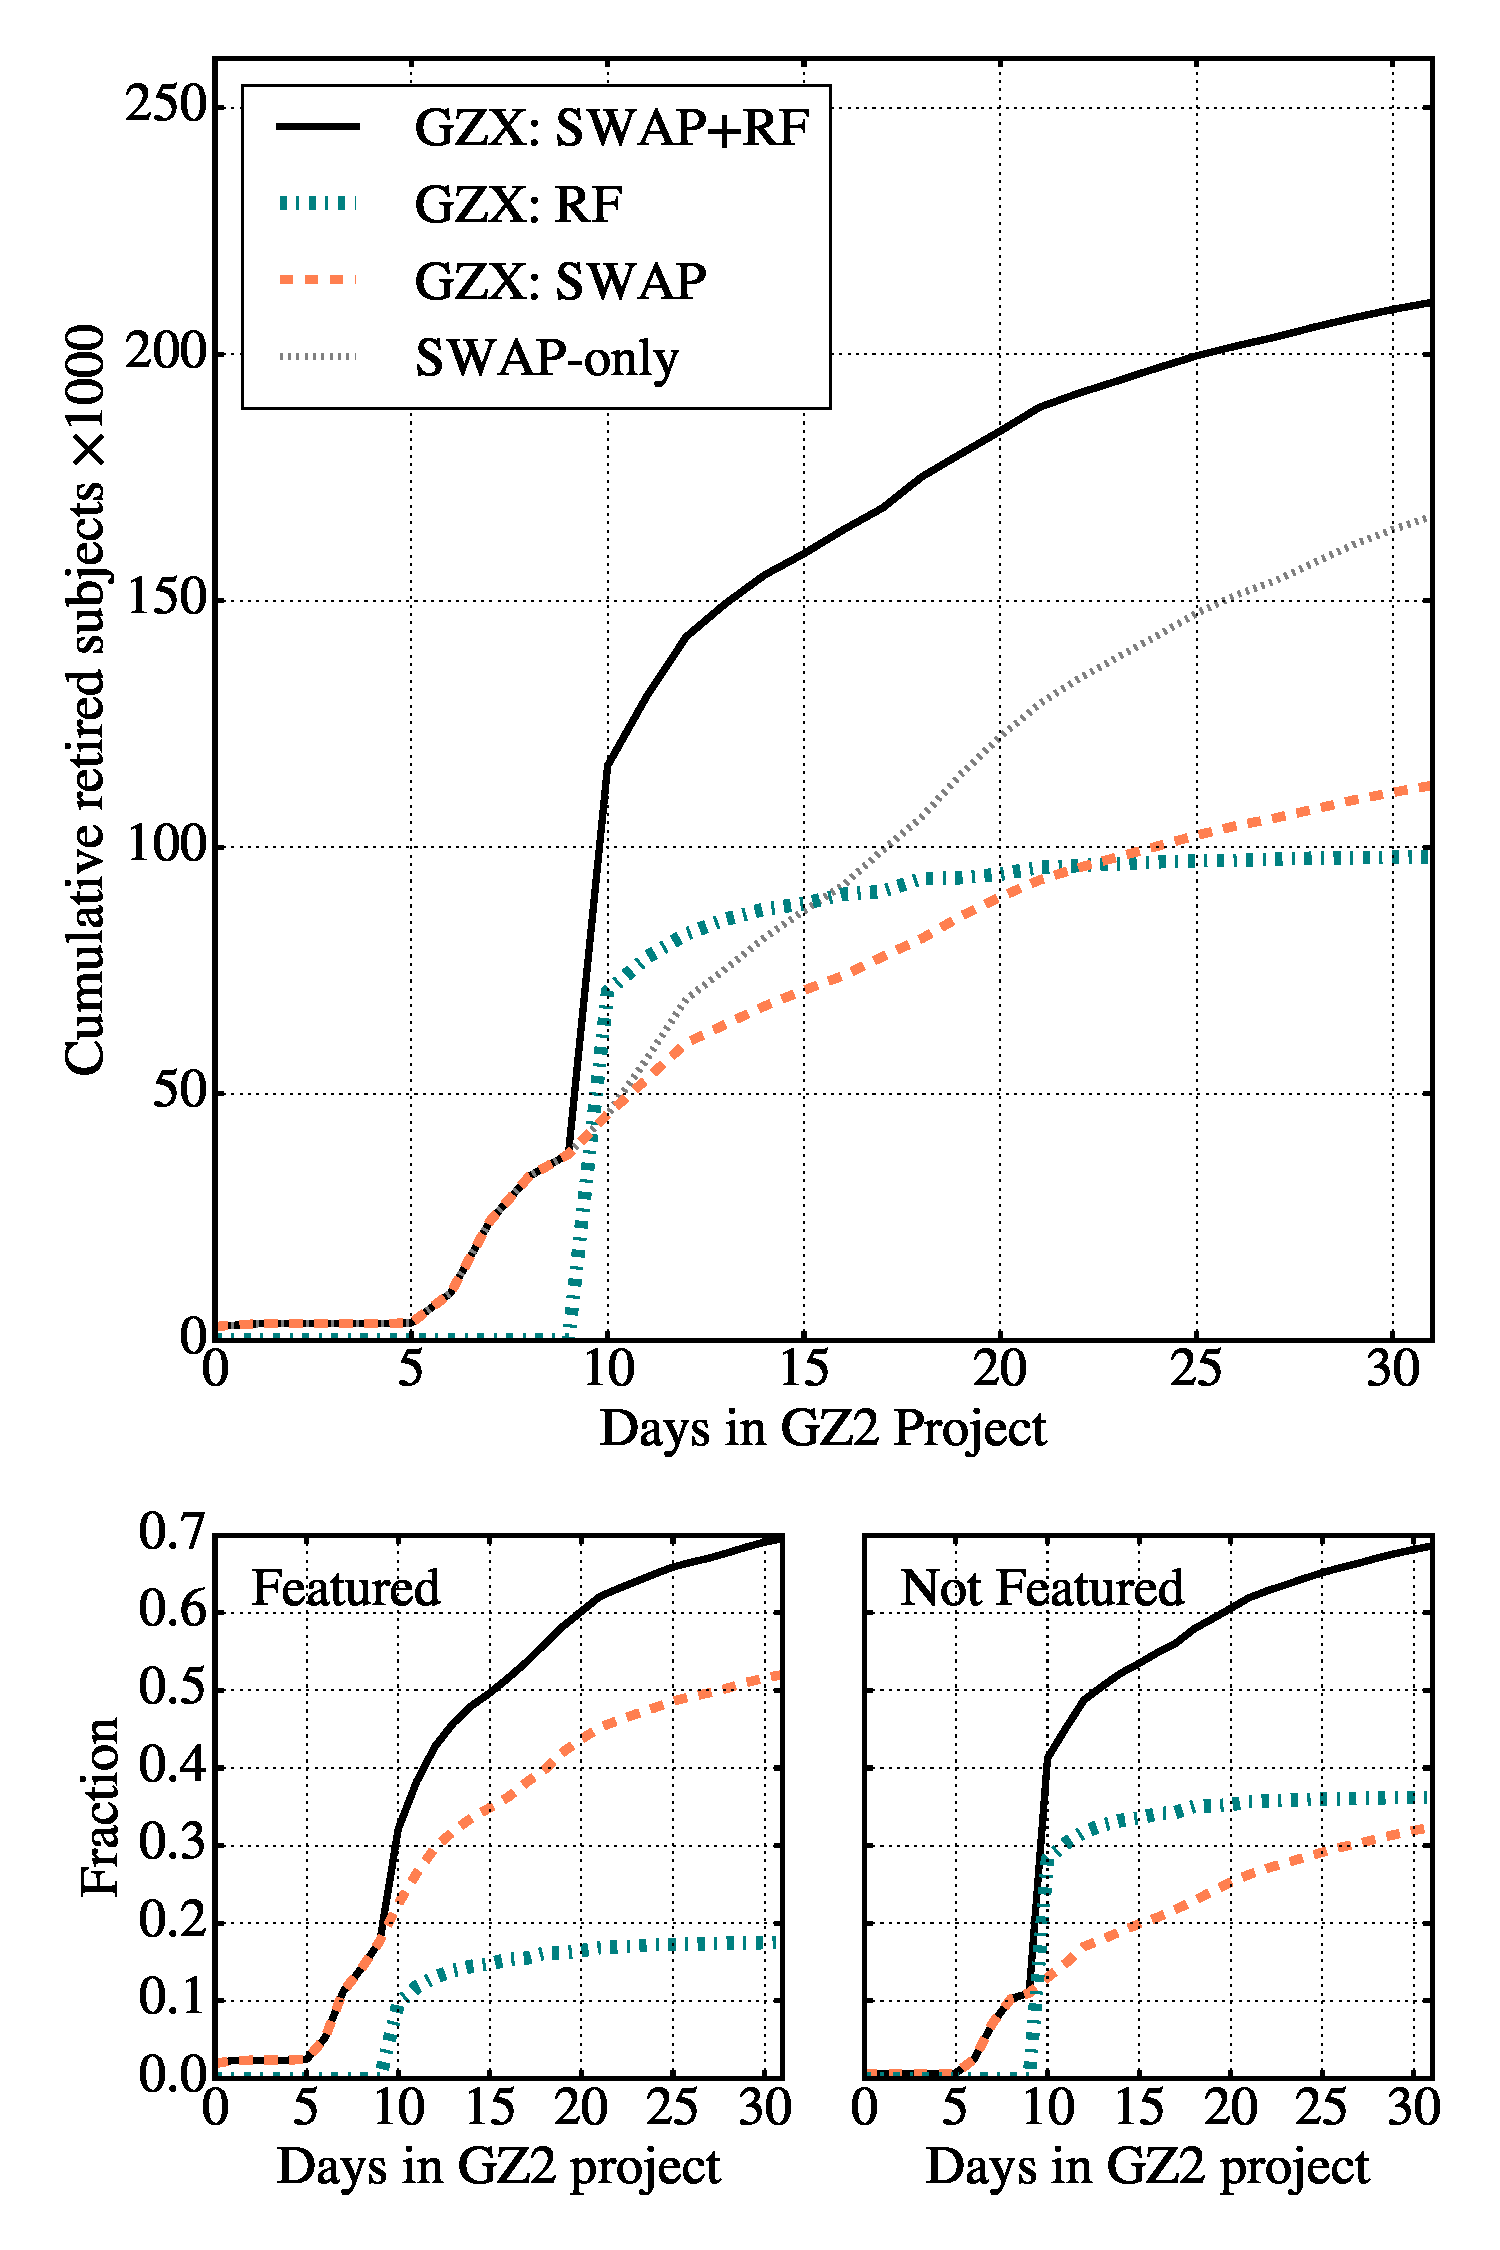
\includegraphics[width=3.5in]{Figures/human_machine/f8.pdf}
\caption[Individual contributions of human and machine to galaxy classification]{Contributions to subject retirement by both classifying agents of GZX: human (SWAP) and machine. The top panel shows cumulative subject retirement for GZX as a whole (solid black), along with that attributed to the RF (dash-dotted teal), and SWAP (dashed orange). The dotted grey line shows the fiducial SWAP-only run for comparison. Retirement totals for humans and machine are nearly equal over the course of the simulation but display different behaviours: SWAP's retirement rate is almost constant while the RF contributes substantially after its initial application and then plateaus.  The bottom panels show what fraction of GZ2 subjects are retired, separated by class label. Overall, GZX retires 73.6\% of the entire GZ2 sample in 32 days, retiring the same proportion of~\feat~and~\notfeat~subjects as indicated by the black lines. However, humans retire 30\% more~\feat~subjects than the machine, while both components retire a similar proportion of~\notfeat~subjects. \label{fig: gzx components}}
\end{figure}


\begin{table*}[]
	\centering
	\caption[Simulation summary]{Summary of key quantities for GZ2 and our various simulations. All quality metrics are calculated using~\raw~labels.}
	\label{tab: summary}
	\let\mc\multicolumn
	\begin{tabular}{lcccccc}
		
		\mc7c{ \textbf{Simulation Summary} } \\
		\hline \hline
			& Days	& Subjects Retired & Human Effort 	&  Accuracy 	& Purity 	& Completeness\\
		\mc2c{} 		& 	 	& (classifications) 	&  (\%)	    	& (\%)	& (\%)	\\
		\hline
			
		Galaxy Zoo 2	&	430 	& 285962  	& 16,340,298 	& --   	& --    	 & --   \\
		SWAP only	&	92    	& 226124          & 2,298,772	& 95.7 	& 86.7	 & 99.0     \\
		SWAP+RF   	& 32  	& 210543 	& 932,017 	& 93.5    	& 84.2    	& 94.3      \\
		\hline
	\end{tabular}
\end{table*}
%%%-------------------------------------------------------
%%%  FIGURE:    MACHINE GETS IT RIGHT!!!
%%%-------------------------------------------------------
\begin{figure*}[t!]
\centering
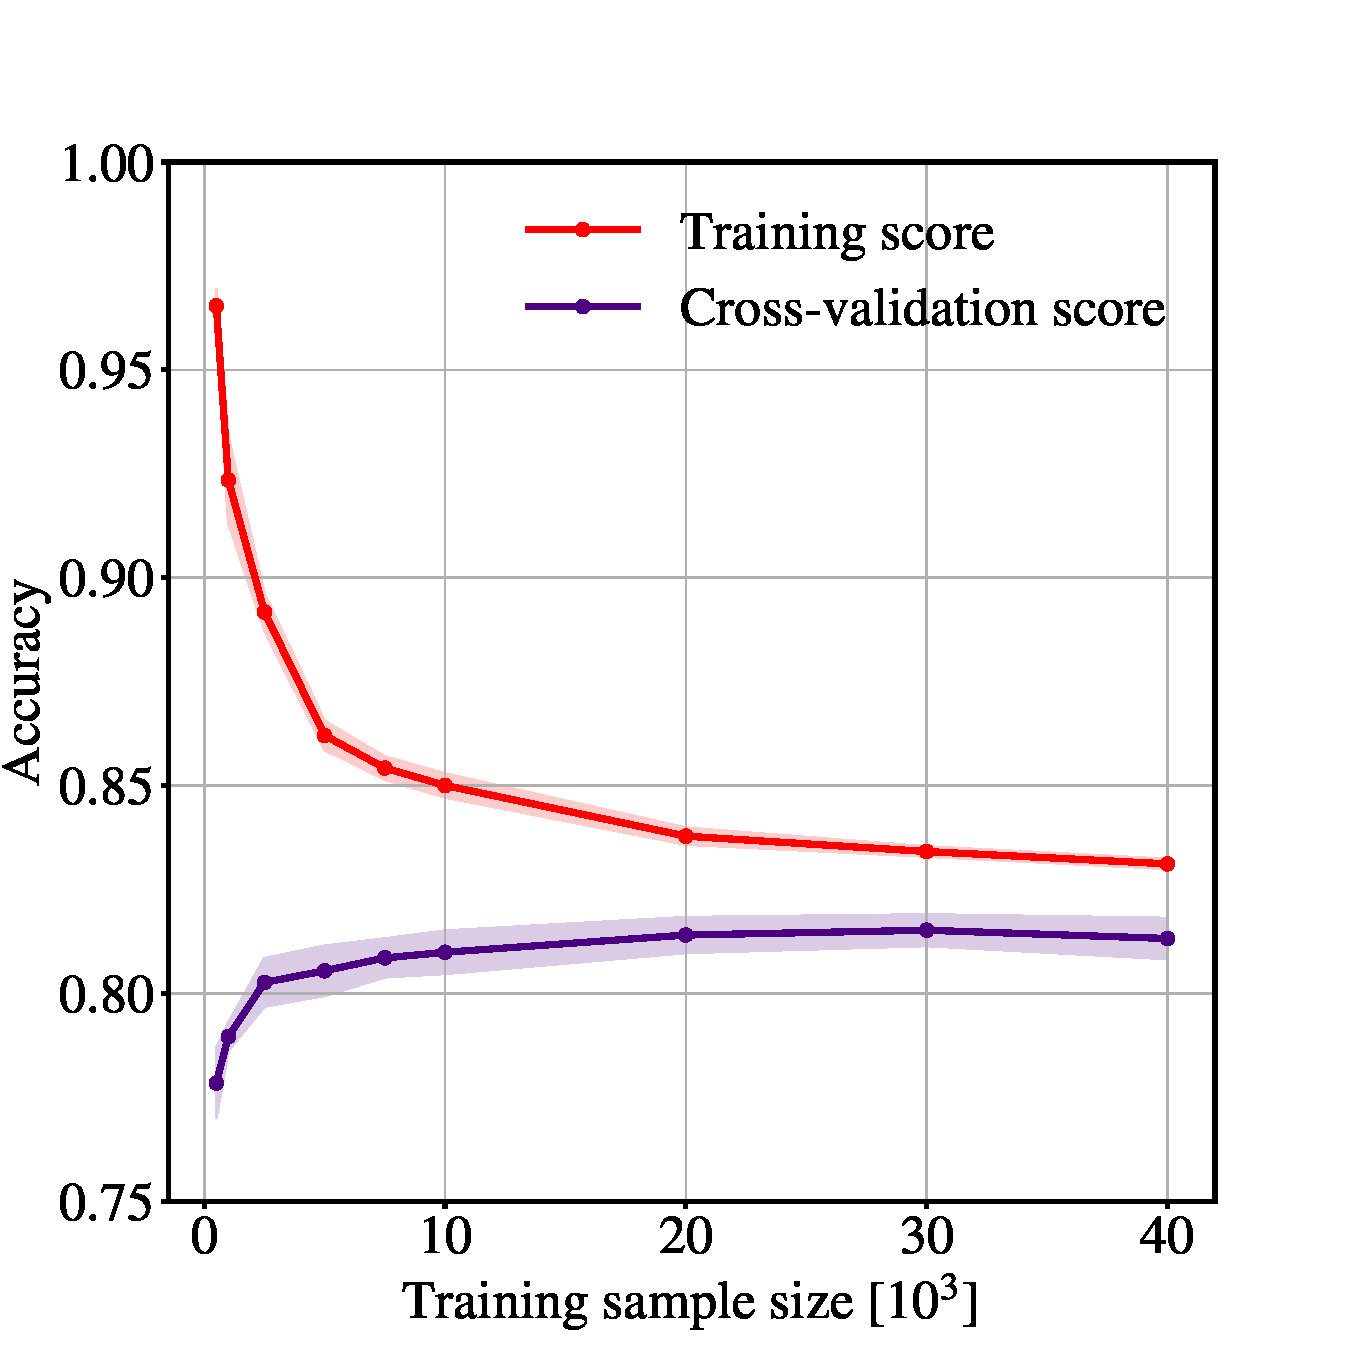
\includegraphics[width=6.5in]{Figures/human_machine/f9.pdf}
\caption[Random subsample of galaxy jpegs identified as false positives by the Random Forest]{A random subsample of subjects identified as false positives: labelled by machine as~\feat, but as~\notfeat~according to~\raw. We display \fsmooth~in the lower left corner, that is, the fraction of volunteers who classified the subject as `smooth' (\notfeat). Values are typically between 0.5 and 0.65 indicating that GZ2 volunteers did not reach a strong consensus. Fortunately, the machine is able to identify these subjects as~\feat~due to their measured morphology diagnostics. \label{fig: machine false pos}}
\end{figure*}


%%%-------------------------------------------------------
%%%  FIGURE:   CAS DISTRIBUTIONS 
%%%-------------------------------------------------------
\begin{figure*}[t!]
\centering
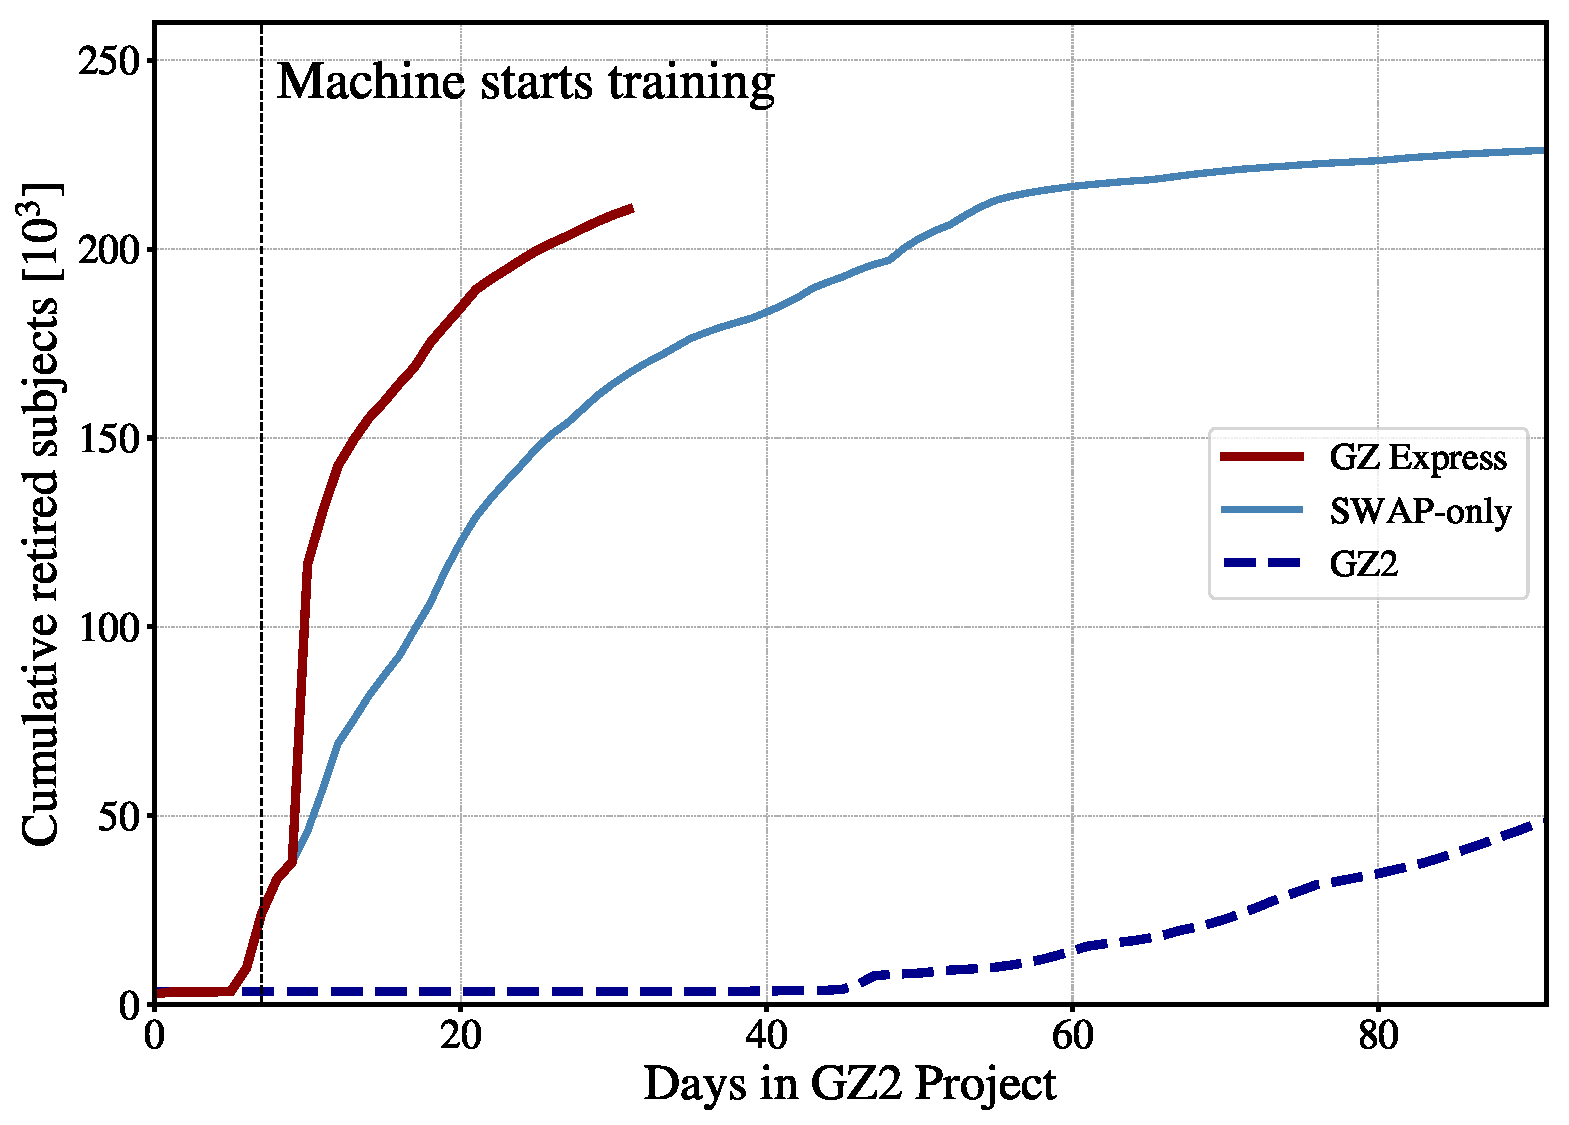
\includegraphics[width=7in]{Figures/human_machine/f10.pdf}
\caption[Distributions of measured galaxy morphology features.]{The RF is trained on a 5-dimensional morphology parameter space. We show the distribution of each morphology indicator for machine-retired~\feat~(blue) and~\notfeat~(orange) subjects compared to the full GZ2 subject sample (black). The difference between~\feat~and~\notfeat~subjects is in stark contrast for all distributions except, perhaps, \M{20}.  \label{fig: morph params}}
\end{figure*}

In the bottom panels of Figure~\ref{fig: gzx components}, we consider the class
composition of subjects retired by SWAP and the RF. 
The left (right) panel shows the retired fraction of GZ2 subjects identified 
as~\feat~(\notfeat) according to their~\raw~labels as a function of GZ2 project time. 
Overall, GZX retires 73.6\% of the GZ2 subject sample and this is evenly 
distributed between~\feat~and~\notfeat~subjects as indicated by the solid
black lines in both panels. 
However, SWAP retires more than 50\% of all~\feat~subjects while the machine
retires only 18\%. This divergence does not exist for~\notfeat~subjects where
each component contributes 33-37\%. 

What is the source of this discrepancy? 
Each night the machine trains on a sample composed consistently of 30-40\%~\feat~subjects but does not retire a similar proportion, indicating
that the 30\% of non-retired~\feat~subjects do not receive high~\pmachine. 
In the following section we explore whether this is an artefact of our choice in machine 
or in the human-machine combination implemented here. 

\subsection{Machine performance}\label{sec: machine performance}

Throughout our analysis we have defined~\feat~and~\notfeat~subjects by 
their~\raw~labels as this was the most compatible choice for comparison with SWAP output.  
However, the machine does not learn in the same way, nor is it presented with the 
same information. Machine and human classifications 
each provide valuable and complementary information for identifying \feat~galaxies.

We isolate the 6127 subjects that were deemed false positives, i.e., galaxies 
retired by the machine as~\feat~that have~\notfeat~\raw~labels, a sample that
comprises only 6.25\% of all subjects the machine retires.
We visually examine several hundred
and assess that, to the expert eye, a majority are, in fact, \feat.  
A random sample is shown in Figure~\ref{fig: machine false pos}. 


That the machine strongly identifies these galaxies as \feat~
(\pmachine~$\ge 0.9$) where humans instead classify them as \notfeat~(\ffeat~$< 0.5$) 
has several contributing factors: 1) as discussed in Section~\ref{sec: swap gz2 disagree}, 
the threshold we chose carries with it a confidence interval such that subjects with 
$0.4 <$~\ffeat+\fstar~$< 0.6$ are most likely to receive disagreeing labels from 
other classifying agents, 2) the first task of the GZ2 decision tree asks a 
question that does not necessarily correlate with a split between early- and
 late-type galaxies, and 3) the machine learns on morphology diagnostics
 that are very different from visual inspection.

We find that 41.4\% of these false positives have $0.4 \le$~\ffeat+\fstar$<0.5$ 
indicating that the disagreement between humans and machine is likely due to the 
labels we assign at our given threshold. However, we also find that 43.5\% of false 
positives have \ffeat+\fstar~$\le0.35$, and this discrepancy is not as easily explained. 
 In Figure~\ref{fig: machine false pos} we examine a random sample of false positives 
in this regime where, for clarity, we display only the \ffeat~value in the lower left corner. 
The majority of these subjects are discs lacking features such as spiral arms or strong bars. 
Whether this is the reason the majority of volunteers classify these objects as 
``smooth" is beyond the scope of this paper, however, this behaviour might be 
modified by providing actual training images and live feedback as performed in
 \cite{Marshall2016}. We suggest that, at least for this particular question, 
if either human or machine identifies a subject as \feat, it is likely the subject 
is discy and worth further investigation.


%%%-------------------------------------------------------
%%%  FIGURE:   FEATURE IMPORTANCES
%%%-------------------------------------------------------
\begin{figure}[t]
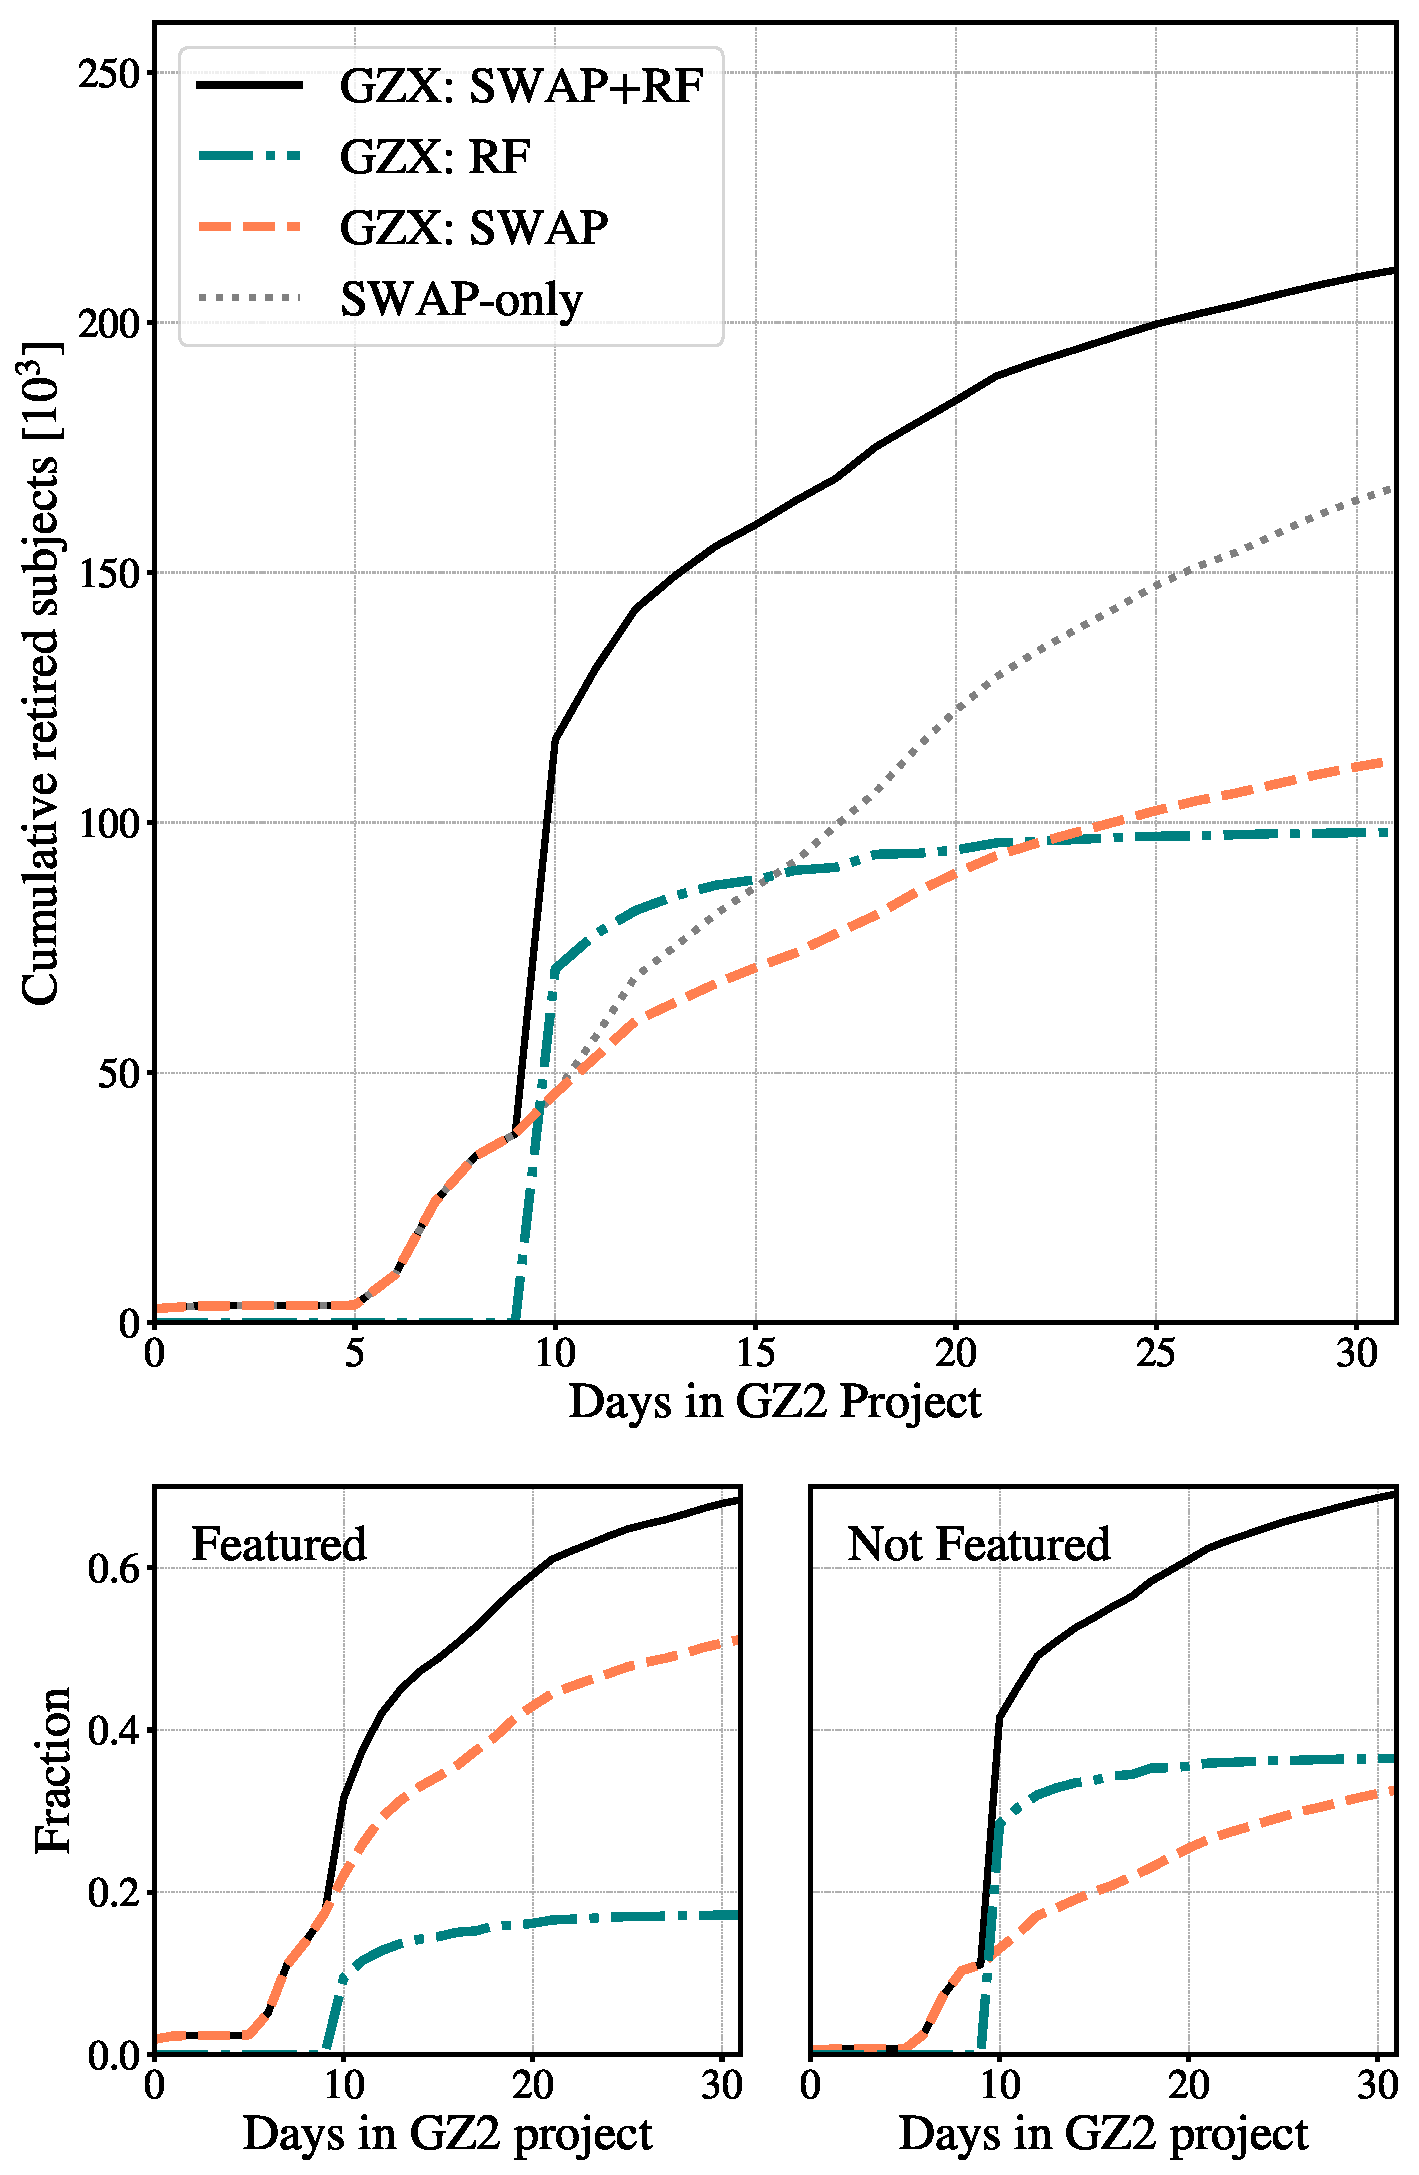
\includegraphics[width=3.5in]{Figures/human_machine/f11.pdf}
\caption[Random Forest's feature importances]{The RF's ranked feature importance averaged over all nights of training with black bars indicating the standard deviation. A larger value corresponds to higher importance. The machine computes feature importance according to how much each feature increases the purity of the resulting split averaged over all trees in the forest. The RF places great importance in the Gini coefficient though we note that it can under-represent the importance of highly correlated features such as concentration.\label{fig: feature importance}}
\end{figure}

Accordingly, this suggests that, in some cases, the morphology indicators we measure are 
sufficient for the machine to recognize~\feat~galaxies regardless of the labels humans provide. 
Figure~\ref{fig: morph params} shows the distribution of each 
morphology indicator for all subjects the machine retires as~\feat~(blue) 
and~\notfeat~(orange) compared to the full GZ2 subject set. 
The difference between~\feat~and~\notfeat~is stark in all but the \M{20} distribution. 
This can be seen explicitly in Figure~\ref{fig:  feature importance} in which
we show the RF's ranked feature importances, where large values indicate higher importance. 
Feature importance is computed as how much each feature decreases the impurity 
of a split in a tree. The impurity decrease from each feature is then averaged over
all trees and ranked. 
We show the feature importance averaged over all nights of training with 
black bars indicating the standard deviation. The machine finds the Gini coefficient 
most important for class prediction, placing little emphasis on \M{20}. 
It is well known that the Gini coefficient is more sensitive to noise than other diagnostics, 
however, we point out that when a machine is faced with two or more correlated features 
any of them can be used as the predictor. Once chosen, the importance of the others is reduced. 
This explains why Concentration is ranked much lower than Gini even though they 
are strongly correlated as seen in Figure~\ref{fig: morph thresh}. 
That the machine relies heavily on these two morphology diagnostics is unsurprising as
concentration has long been an automated predictor between early- and late-type galaxies~\citep{Abraham1994, Abraham1996, Shen2003}.


The complementary nature of human and machine classification can 
best be utilized by a feedback mechanism in which a portion of machine-retired
subjects are reviewed by humans. Subjects that display excessive disagreement
should be verified by an expert (or expert-user).  In the same way that 
humans increase the machine's training sample over time, subjects that the
machine properly identifies can become part of the humans' training sample. 



%%----------------------------------------------------------------------------------------------------------------------------------------------------
%%   MAD RAVINGS OF THE FUTURE 
%%----------------------------------------------------------------------------------------------------------------------------------------------------
\section{Looking Forward}\label{sec: visions}

We have demonstrated the first practical framework for combining human and machine
 intelligence in galaxy morphology classification tasks. 
While we focus below on a brief discussion of our next steps and potential applications
to large upcoming surveys, we note that our results have implications for the future
of citizen science and Galaxy Zoo in particular. 


GZX is perhaps one of the simplest ways to combine human and machine intelligence
 and its impressive performance motivates a higher level of sophistication. 
A first step will be an implementation of SWAP that can handle a complex decision tree. 
In addition, we envision multiple forms of active feedback in addition to 
our passive feedback mechanism.  SWAP allows us to leverage the 
most skilled volunteers to review galaxies difficult for either
 human or machine to classify.  Additionally, machine-retired subjects should 
contribute to the training sample for humans in an analogous fashion to what 
we have already implemented. 


Secondly, our RF can be improved by providing it information equal to what
humans receive: multi-band morphology diagnostics will be
included in our future feature vector.  However, the Random Forest algorithm is not 
easily adapted to handle measurement errors or class labels with continuous distributions. 
To fully utilize the information provided by SWAP, sophisticated algorithms should be considered such as 
deep convolutional neural networks (CNN) or Latent Dirichlet allocation (LDA), 
an algorithm that is frequently used in document processing.  
Furthermore, there is no reason to limit to a single machine. 
As hinted at in Figure~\ref{fig: schematic}, several machines could train simultaneously, 
their predictions aggregated through SWAP, creating an on-the-fly machine ensemble.

%%----------------------------------------------------------------------------------------------------------------------------------------------------
%%  IMPLICATIONS FOR UPCOMING LARGE-SCALE SURVEYS
%%----------------------------------------------------------------------------------------------------------------------------------------------------

With the above upgrades implemented, we expect performance of both the
classification rate and quality to further increase. However, even our current 
implementation can cope with upcoming data volumes from large surveys. 
By some estimates, \textit{Euclid} is expected to obtain measurable morphology with its 
visual instrument (VIS) for approximately $10^6 - 10^7$ galaxies~\citep{Euclid}.
Visual classification at the rate achieved with Galaxy Zoo today
would require 12--120 years to classify.\footnote{We note that the classification 
rate of GZ2 was 4 times higher than GZ's current steady rate.}
If the \textit{Euclid} sample is on the high end, GZX as currently implemented
could classify the brightest 20\% during the six years of its observing mission. 
As currently implemented, we obtain accuracy around 95\% potentially leaving
hundreds of thousands of galaxies with unreliable classifications.  
In a companion paper that seeks to identify supernovae, Wright et al. (submitted) 
demonstrate a dramatic increase in accuracy through an entirely different human-machine 
combination whereby the
scores from human and machine are averaged together with the combined score 
yielding the most reliable classification. Again, a combination of both 
approaches will allow us to take full advantage of legacy output from large scale surveys.


%%----------------------------------------------------------------------------------------------------------------------------------------------------
%%   CONCLUSIONS 
%%----------------------------------------------------------------------------------------------------------------------------------------------------
\subsection{Conclusions}

In this paper we design and test Galaxy Zoo Express, an innovative system\footnote{Our code can be found at \url{https://github.com/melaniebeck/GZExpress}} 
for the efficient classification of galaxy morphology tasks that integrates the 
native ability of the human mind to identify the abstract and novel with 
machine learning algorithms that provide speed and brute force.  
We demonstrate for the first time that the 
SWAP algorithm, originally developed to identify rare gravitational lenses in the 
Space Warps project, is robust for use in galaxy morphology classification. 
We show that by implementing
SWAP on GZ2 classification data we can increase the rate of classification by a factor
of 4-5, requiring only 90 days of GZ2 project time to classify nearly 80\% of the
entire galaxy sample. 

Furthermore, we have implemented and tested a Random Forest algorithm 
and developed a decision engine that delegates tasks between human and 
machine.  We show that even this simple machine is capable of providing significant 
gains in the classification rate when combined with human classifiers: GZX
 retires over 70\% of GZ2 galaxies in just 32 days of GZ2 project time.  
This represents a factor of 11.4 increase in the classification rate as well as
 an order of magnitude reduction in human effort compared to the original GZ2 project. 
This is achieved without sacrificing the quality of classifications as we maintain 
accuracy well above 90\% throughout our simulations. 
Additionally, we have shown that training on a 5-dimensional parameter space of 
traditional non-parametric morphology indicators allows the machine to identify 
subjects that humans miss, providing  a complementary approach to visual classification. 
The gain in classification speed allows us to tackle the massive amount of data promised
 from large surveys like \textit{LSST} and \textit{Euclid}.
 
 
%%----------------------------------------------------------------------------------------------------------------------------------------------------
%%   ACKNOWLEDGEMENTS
%%----------------------------------------------------------------------------------------------------------------------------------------------------
\section{Acknowledgements}
MB thanks Steven Bamford and Boris H{\"a}u{\ss}ler for insightful discussions on citizen science and Galaxy Zoo; and John Wallin and Marc Huertas-Company for several enlightening conversations on machine learning and classification. 
We are grateful to Elisabeth Baeten, Micaela Bagley, Karlen Shahinyan, Vihang Mehta, Steven Bamford, Kevin Schawinski, and Rebecca Smethurst for providing expert classifications in addition to those provided by the authors. PJM acknowledges Aprajita Verma and Anupreeta More for their ongoing collaboration on the Space Warps project. 

MB, CS, LF, KW, and MG gratefully acknowledge support from the US National Science
Foundation Grant AST-1413610.  MB acknowledges additional support 
through New College and Oxford University's Balzan Fellowship as well as the University
of Minnesota Doctoral Dissertation Fellowship. Travel funding was supplied 
to MB, in part, by the University of Minnesota Thesis Research Travel Grant. CJL recognizes support from a grant from the Science \& Technology Facilities Council (ST/N003179/1). 
BDS acknowledges support from Balliol College, Oxford, and the National Aeronautics and Space Administration (NASA) through Einstein Postdoctoral Fellowship Award Number PF5-160143 issued by the Chandra X-ray Observatory Center, which is operated by the Smithsonian Astrophysical Observatory for and on behalf of NASA under contract NAS8-03060. The work of PJM is supported by the U.S. Department of Energy under contract number DE-AC02-76SF00515.

%!TEX root = thesis.tex

\chapter{A population of ``clumpy'' galaxies in local Universe}\label{chap:5}
Simultaneous to the development of this research was the publishing of the Galaxy Zoo: Hubble galaxy morphology classification catalog. A portion of the original GZ2 SDSS galaxy sample was included in Galaxy Zoo: Hubble because the decision tree for the latter was more complex than that for GZ2. This enabled a comparison between different decision trees and led to the identification of a rare sample of low redshift clumpy galaxies. This chapter details the identification of such a sample, preliminary analysis of the star-forming clumps, and methods to identify more such galaxies in the local universe as these may be analogs of high redshift galaxies with similar properties.


\section{Introduction}
Structural properties of typical galaxies today wereforgedover the5billionyearsbetween the peakof the cosmic star-formation history at z ⇠ 1.5  2 and now.From the theoretical perspective,galaxies’ growth is predominantly governed by the baryonic physics of gas accre-tion and energy feedback, rather than by merg-ers that induce starbursts (e.g., Somerville and Dav ́ e, 2015). Gas inflow modulates galaxies’ star formation history and plays a crucial role in the dynamical state of the galaxy.A varying gas fraction changes the amount of fragmentation within the gaseous disk, the star-formation rates (SFR), strengths and lifetimes of disk structural components, and possibly the fueling rate of the AGN. As a consequence of the gas accretion pro-cess, the small-scale structure within disk galax-ies is also predicted to change over time, with the appearance of stable “grand design” spiral arms only at later epochs (e.g. Oppenheimer et al., 2010; Bouch ́ e et al., 2010; Dav ́ e et al., 2011a,b; Lilly et al., 2013; Hirschmann et al., 2013). 

n the theoretical paradigm discussed above, the origin of these massive clumps is still an open debate. Two main physical scenarios have been proposed.On one side (hereafter referred to as in-situ models),giant clumps are expectedto form inside pre-existing galaxies.In these sce-narios, haloes located at the center of multiple filaments continuously accrete gas from the cos-mic web.This accretion results in the forma-tion of gas-dominated disks that eventually frag-ment into giant clumps by gravitational insta-bility (Bournaud et al., 2007; Dekel et al., 2009; Behrendt et al., 2015). On the other side (here-after referred to as ex-situ models) clumps may have an external origin, as in the case of mergers with small star-forming companions (Ceverino et al., 2010; Bournaud, 2016). 

Observationally, the situation is still unclear. The large gas-to-baryonic fraction of 20 to 80 recently measured with interferometric studies in clumpy galaxies lends support to the in-situ models(e.g., Erb et al., 2006; Tacconi et al., 2008, 2010).Similarly, the kinematics in the majorityofthesegalaxiesischaracterized by large, regularly-rotating disks, with no signs of on-going or recent mergers (Genzel et al., 2006; F ̈ orster Schreiber et al., 2009; Epinat et al., 2012; Newman et al., 2012).These studies, however, are 1) limited to galaxies with SFR> 10M yr 1 and M>10 10 M) and 2) include only a few galaxies with high spatial resolution kinematic and interferometric data (Genzel et al., 2014). 

The lack of existing observational constraints below 10 10 M is of particular concern. It is pre-cisely in this mass range that most of the con-straining power resides. In fact, state of the art simulations that directly resolve the interstellar medium of individual galaxies while capturing their cosmological environment show that low mass galaxies are the mostly a↵ected by preven-tive feedback (e.g., FIRE Muratov et al.2015; 11
GASOLINE Christensen et al. 2015; and MU-FASA Dav ́ e et al.2016).These simulations show that in galaxies with M<10 10 supernova-driven fast outflows can lower the gas inflow rate, and consequently the rate at which clumps are formed in-situ, compared to more massive galax-ies. If clumps are the result of minor merging, on the other hand, the dependency with stellar mass would depend on the specifics of the dy-namics of the mergers. 

Throughout this chapter we assume a flat Planck cosmology with H$_0=67.8$ and $\Omega_m = 0.308$ where appropriate. 


\section{Sample Selection \& Data} \label{sec:chap5-sample}

We identify a sample of clumpy galaxies in the local universe by considering classifications from both the Galaxy Zoo 2 \citep[GZ2][]{Willett2013} and Galaxy Zoo: Hubble \citep[GZH][]{Willett2017} projects. We provide a brief overview of each of these projects here. 

The GZ2 subject sample consists of 285,962 galaxies identified as the brightest 25\% ($r$-band magnitude $< 17$) residing in the SDSS North Galactic Cap region from Data Release 7 and included subjects with both spectroscopic and photometric redshifts out to $z < 0.25$. In addition to the DR7 Legacy catalog, galaxies were included from Stripe 82, a multiply-imaged strip along the celestial equator in the Southern Galactic Cap. Galaxies in this region were selected to have $m_r\le17.7$ and petror90\_r $>3$, where petror90\_r is the radius containing 90\% of the r-band Petrosian aperture flux.


\begin{figure}
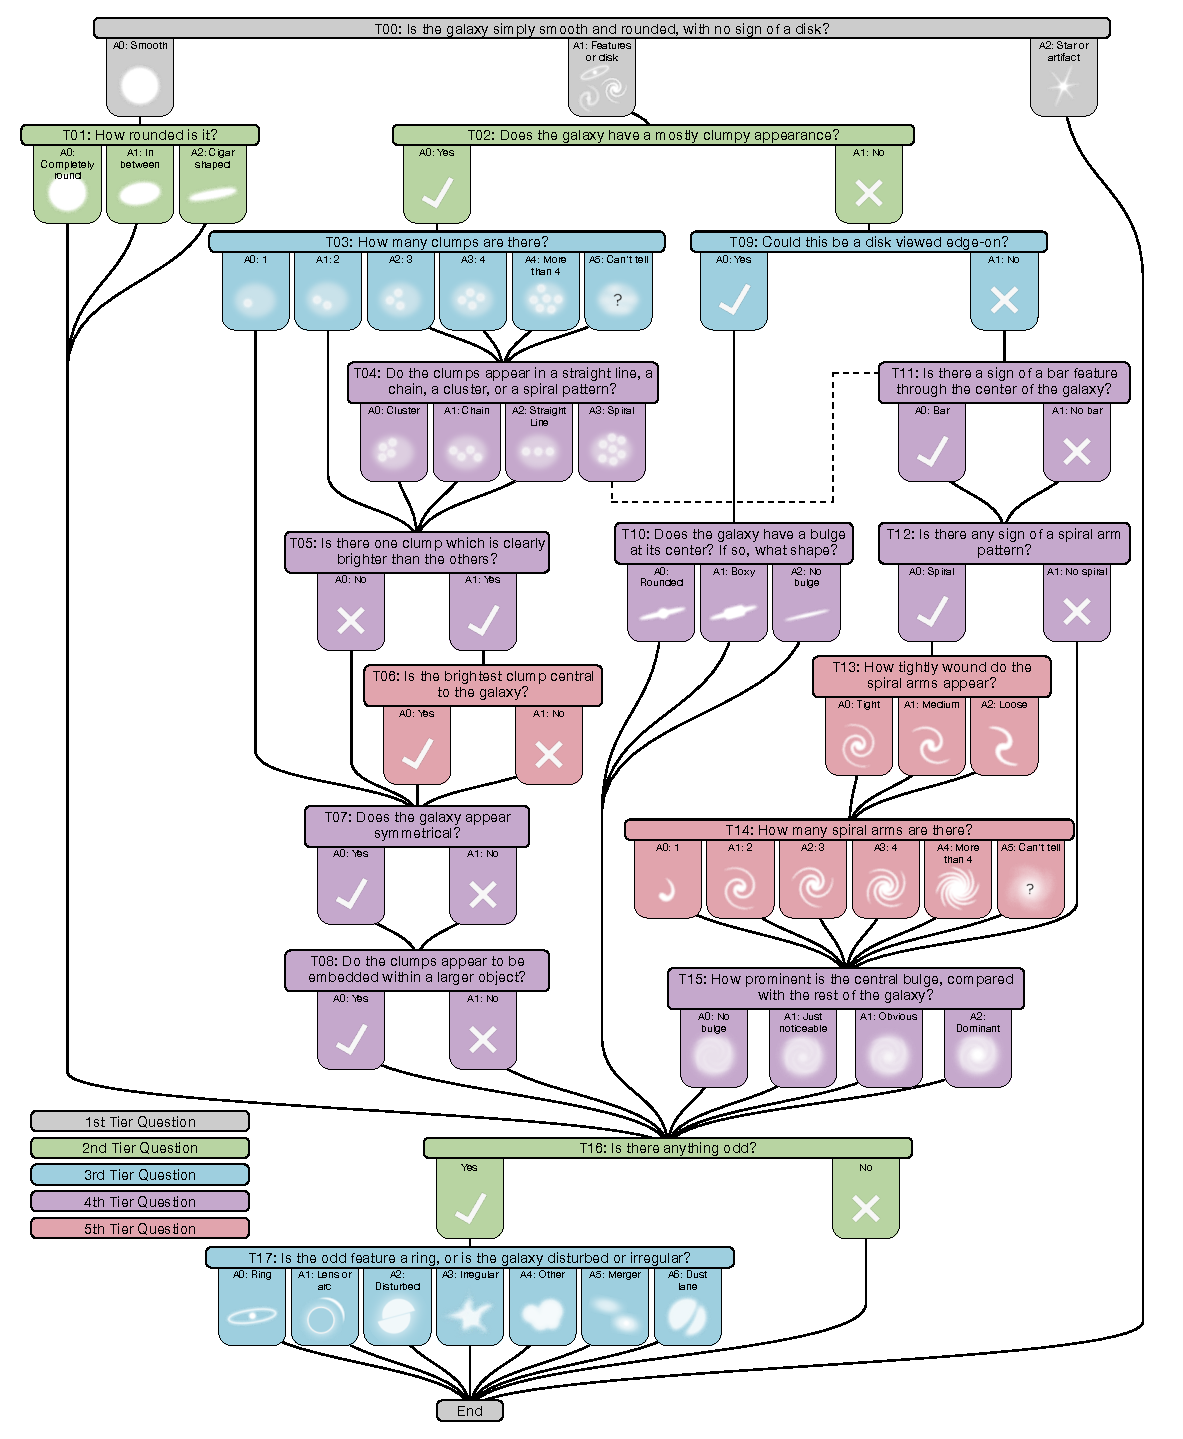
\includegraphics[width=\textwidth]{Figures/gz3_tree_resized.pdf}
\caption[Galaxy Zoo: Hubble decision tree.]{Galaxy Zoo: Hubble decision tree. The most notable difference between this decision tree and that used during the Galaxy Zoo 2 project is the ``clumpy'' branch of tasks.}
\label{fig: gzh decision tree}
\end{figure}

The GZH project contains images drawn from several dedicated surveys and sample selection criteria. Most samples are drawn from various Hubble fields such as AEGIS, GOODS and COSMOS; however also included are the single-epoch and co-added images from Stripe 82 of the SDSS Data Release 7 that were part of the GZ2 project. The single-epoch imaging allows for local comparison to higher redshift galaxies, while the co-added imaging allows for image depth analyses. 

The most notable difference between these two projects is the decision tree presented to volunteers. The goal of GZH was to collect detailed morphologies for galaxies in Hubble imaging which extends to much higher redshift than those of the SDSS sample. Galaxies at higher redshift do not necessarily follow the traditional Hubble sequence and thus a new branch of questioning was added to the decision tree for this project, shown in Figure \ref{fig: gzh decision tree}. This included several questions concerning the clumpy nature of galaxies, a morphological feature well known to exist at higher redshift. Because GZH included galaxies from the GZ2 project, we can draw on both sets of decision trees to identify clumpy features for galaxies in Stripe 82.


To select a sample of ``clumpy" galaxies from the GZH Stripe 82 sample, we consider only those subjects with large featured (\ffeat) and clumpy (\fclump) vote fractions: the fraction of volunteers who voted a subject as `featured or disk' in response to the first question ``Is the galaxy simply smooth and rounded, with no sign of a disk?'' and who answered `yes' to the question ``Does the galaxy have a mostly clumpy appearance?'' Specifically, we select galaxies which satisfy \ffeat~$\ge0.5$ and \fclump~$\ge0.5$ Additionally, we require $N_{\mathrm{votes}} \ge 20$, where $N_{\mathrm{votes}}$ is the number of volunteers who answerd the clumpy question. This insures that \fclump~is statistically significant and not a product of too few votes.  This yields a sample of 629 galaxies: 273 single-epoch imaging and 356 from the co-added imaging. After visual inspection we find that this is hardly a pure sample of clumpy galaxies in the traditional sense, instead including a sizeable sample of tight groups of elliptical galaxies, as well as galaxies in various merging states, possessing multiple nuclei. [\textbf{show example image?}] After excluding these and duplicate imaging, we retain 92 coadd-depth and 105 single-depth clumpy galaxies, of which 156 are unique systems (some objects are common to both the single-epoch and coadd-depth imaging). Finally, we exclude galaxies with $z>0.06$ in order to retain a sample wherein the physical scale as observed by SDSS is similar to Hubble's at $z\sim3$ to allow for comparison with high redshift samples. Our final sample contains 105 unique galaxies. 

\begin{figure}
\centering
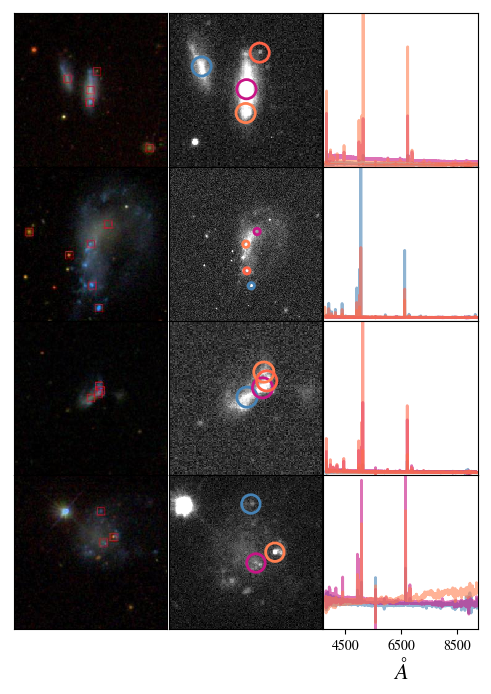
\includegraphics[width=4.75in]{Figures/jpeg_fits_spec_examples.png}
\caption[Sample of ``clumpy'' galaxies determined by Galaxy Zoo: Hubble]{Sample of ``clumpy'' galaxies. The first column shows the SDSS $gri$ color composite image where the red squares denote locations of SDSS spectroscopy. The middle column shows our postage stamp for the object where the colored circles show the same spectral locations, however these circles are color coded to the third panel which shows the spectra associated with each object.}
\label{fig: clumpy examples}
\end{figure}

We obtain SDSS Data Release 12 (DR12) \textit{ugriz} coadd imaging, as well as all optical spectra associated with each galaxy. The wavelength range of the SDSS spectra is $3800-9200$\AA~with a resolution of $R\sim 1500$ at $\sim3800$\AA. The $3$\arcsec~SDSS fibers cover 2.9 kpc at $z=0.05$. We visually inspect all spectra to verify that they are associated with an object in our sample as opposed to a nearby object or overlapping star. Through this inspection we determine that one clumpy galaxy is actually a juxtoposition of three galaxies at disparate redshifts flagged as clumpy in GZH due to the low resolution of SDSS imaging. We exclude this subject from our sample. Our final list includes 171 spectra. Approximately half of the galaxies in our sample have more than one spectrum with a handful having three or four spectra. Figure \ref{fig: clumpy examples} shows some examples of our clumpy galaxies where the first column is the $gri$ color composite SDSS jpeg image with red squares denoting the location of SDSS spectra, the middle column is the $r$-band postage stamp (described below) where the colored circles again denote the location of SDSS spectra and reflect the size of the fiber. The third column shows the spectra associated with each object, color-coded to the apertures in the middle column. 


We create postage stamps of each galaxy from the $r$-band SDSS fields.  The size of the postage stamp is taken to be 3$\times\mathtt{petrorad\_r}$, the Petrosian radius as measured in the $r$-band by the SDSS pipeline. We then run Source Extractor \citep{sextractor} on each postage stamp. During visual inspection of these cutouts and the associated SExtractor segmentation maps we discover that the SDSS coordinates are occasionally incorrectly assigned, that is, star-forming clumps are mistaken for individual galaxies likely due to the low surface brightness of some of these systems. An example is shown in the final row of Figure \ref{fig: clumpy examples}. It is clear in the first panel that the central coordinates are not well aligned with the galactic center. The middle panel depicts our postage stamp in which we have corrected the galaxy's coordinates using that determined by SExtractor. 


We also draw on the \textit{GALEX}-SDSS-\textit{WISE} Legacy Catalog \citep[GSWLC,][]{Salim2016} which provides stellar mass, star formation rates (SFR) and dust attenuations for 700,000 low-redshift galaxies. Specifically we obtain the GSWLC-X version which contains measurements using the deepest imaging available for each galaxy in the sample. We provide a brief overview of their methodology here.  Galaxy physical properties were obtained from UV and optical spectral energy distribution (SED) fitting utilizing imaging data from the \textit{Galaxy Evolution Explorer}, SDSS, and \textit{Wide-field Infrared Survey Explorer} surveys for galaxies with $z<0.3$, covering up to 90\% of the SDSS footprint. \cite{Salim2016} use a Bayesian fitting methodology that includes corrections for photometry blending and emission-line.  We match our sample against this catalog to objects within $15\arcsec$, of which we find 95. Of these, 6 are flagged as having failed the SED fitting and are thus excluded. Thus we retain 89 galaxies with estimates of global galactic paramters. Figure \ref{fig: clumpy gswlc properties} shows the distribution of our sample wherein we plot the galaxy log stellar mass as a function of redshift with color denoting the log SFR. The median galaxy log stellar mass and SED SFR are $\sim$9 M$_{\odot}$ and XXX, respectively. 

\begin{figure}
\centering
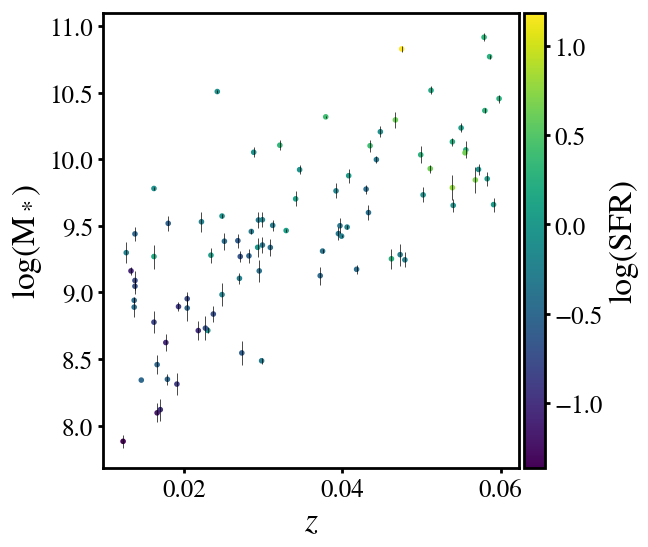
\includegraphics[width=5in]{Figures/mass_z_sfr.png}
\caption[Stellar mass, redshift, and Star-formation rate for a subset of our ``clumpy'' galaxies as measured by the GSWLC.]{Stellar mass, redshift, and star-formation rate (SFR) for a subset of 89 ``clumpy'' galaxies as measured by the GSWLC \citep{Salim2016}.}
\label{fig: clumpy gswlc properties}
\end{figure}

%The physical scale at z= 0.06 is 1"=1.1kpc. SDSS pixel scale is 0.396"/pixel. --> 0.43 kpc/pixel -->  ~2.3 pixels = 1kpc.  We visually inspect these spectra and verify that the fiber was positioned over a star-forming region in the majority of cases rather than the galactic bulge or other structure. 



\section{Are these star-forming regions analogs of high-redshift clumps?}
Many studies have been conducted (cite cite cite) comparing local HII regions to high-redshift star-forming clumps and the debate between whether these regions arise due to the same physical processes is still under debate. In this section we use the GSWLC and spectral features as measured by SDSS to explore various properties of the clumps in our sample. 


\subsection{Clump galactic radial distance} \label{subsec:radii}

Most SDSS fibers are either centered on a bright star-forming region or on/near the galactic center. We thus compute the galactocentric distance of each fiber from the galaxy center and normalized by the galaxy's half light radius (\texttt{FLUX\_RADIUS}) as determined by SExtractor. The resulting distribution is shown in the third panel of Figure \ref{fig: clump properties}. That the distribution is obviously skewed towards the small galactocentric values is likely due to the several spectra that are not covering a clump but instead probe the central region.  

 The \ha~equivalent width is a rough stand-in for specific SFR since it is the ratio of a strong star formation indicator (\ha~line flux) and a reasonable proxy for stellar mass, i.e., the stellar continuum at \ha \citep{MarmolQueralto2016}. However, we find no relation between EW(\ha) and clump radial distance. More telling would be a trend between clump radial distance and stellar age as this diagnostic will potentially distinguish between \textit{in situ} and external clump origin theories. The high quality of the SDSS spectra will allow for detailed stellar age estimates in a future analysis.  

\subsection{Clump luminosity}
We use the \ha~flux as measured by a Gaussian fit to the \ha~emission line to compute the star-formation rate using the well known calibration \citep[e.g.,][and references therein]{Calzetti2013}

\begin{equation}
\mathrm{SFR} (\mathrm{M}_{\odot} \mathrm{yr}^{-1}) = 5.5 \times 10^{-42}L(\mathrm{H}_{\alpha}) (\mathrm{ergs\ s}^{-1})
\end{equation}
 We can then compare SFRs between those derived from the \ha~emission and the global SED SFR. For each galaxy in the sample, we sum the SFR$_{\mathrm{H}_{\alpha}}$ from each spectrum and compare that to SFR$_{\mathrm{SED}}$, for those 89 galaxies that were matched to the GSWLC. Of those, we find the median ratio of the two star-formation measures is $\sim$10\%, with a majority of galaxies having only one spectrum which we interpret as one clump. This rough estimate is not dissimilar to giant star-forming regions found at high redshift where it is typical for individual clumps to contribute 10\% or more to the total star formation of the galaxy \citep{Genzel2011, Guo2012, Wisnioski2012}

\subsection{Velocity dispersion and clump diameters}

In the first panel of Figure \ref{fig: clump properties} we show the distribution of the \ha~velocity dispersion as measured by the SDSS spectroscopic pipeline, where the instrument resolution is subtracted in quadrature. The median for our sample is $\sigma_{\mathrm{H}_{\alpha}}\sim40$km/s and while this is slightly smaller than giant star-forming regions observed at $z\sim$2 (Sanchez et al., 2013; Elmegreen and Elmegreen, 2010), it is also significantly larger than typical HII regions observed in local galaxies (cite cite cite).

%A relationship between clump luminosity and velocity dispersion has been observed and it has been suggested that star formation drives the large observed line widths. In particular, Lehnert postulate that the velocity dispersion is due to mechanical energy released by star formation and that $\sigma$ is proportional to the star formation surface density. Another possibility is that the KS relation holds for star-forming regions


\begin{figure}
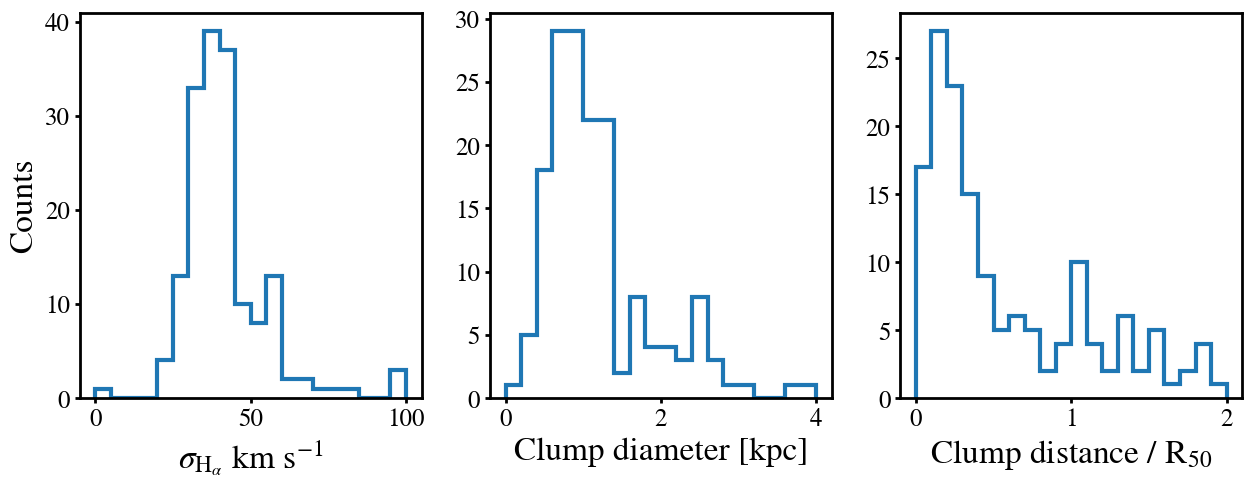
\includegraphics[width=\textwidth]{Figures/clump_properties.png}
\caption[Properties of ``clumps'': velocity dispersion, clump diameter, and clump galactic radial distance.]{Clump properties. }
\label{fig: clump properties}
\end{figure}


%\subsection{Clump diameters}
%If clumps form through disk instabilities as is traditionally thought, the relation between clump velocity dispersion and physical size can be theoretically derived as detailed in \citep[e.g.,][]{Wisnioski2012}, which we briefly review here. 

\cite{Wisnioski2012} develop empirical relations between clump size, luminosity, and velocity dispersion for a sample of local HII regions along with a sample of high redshift clumps. They demonstrate that these relations hold over three orders of magnitude in clump diameter and five orders of magnitude in \ha~luminosity for thousands of local HII regions and high-redshift clumps taken from 11 different studies. Specifically, we invert the following relation to estimate the clump diameter from the SDSS measurement of the \ha~velocity dispersion

\begin{equation}\label{eqn: clump diameter}
\log(\sigma) = (0.42 \pm 0.03) \times \log(d) + (0.33 \pm 0.09)
\end{equation}

The resulting clump diameter distribution is shown in the middle panel of Figure \ref{fig: clump properties}. The median diameter is $\sim$1 kpc which is larger than the average local HII region but slightly smaller than high redshift clumps.  Keep in mind that some of these ``clumps'' could actually be the central bulge region of some of these systems as we do not specifically separate the two so as to bias against the possibility of older (and hence redder, less star formation) clumps at smaller galactic radius. The central regions will typically have much lower rates of star formation as measured by \ha~and subsequently, smaller velocity dispersion, and thus they will have significantly smaller sizes according to this relation. In a more detailed analysis, clump sizes should be confirmed independently through a ``core'' analysis whereby clump sizes are measured by fitting a Gaussian to the 1D radial surface brightness profile of each star-forming region.  
%% If you wish to include an acknowledgments section in your paper,
%% separate it off from the body of the text using the \acknowledgments
%% command.



In future analyses, the quality of the SDSS spectra will allow for the derivation of accurate stellar ages from fitting of the continuum, as well as gas metallicity (e.g., Henry et al., 2015). With these measurements we can begin to study statistical properties that correlate with clump galactocentric distance. 

\section{Summary}


Though preliminary, this analysis demonstrates that star-forming regions in this galaxy sample are likely more similar to high-redshift clumps than to typical local HII regions. This motivates not only a more in depth analysis of this sample but also justifies the search for similar galaxies in the local universe. These clumpy galaxies were found as a consequence of SDSS Stripe 82 galaxies being included in the GZH project. We next detail a new project that will potentially find an order of magnitude more galaxies similar to the sample presented here.


%=========================================================================
%	CLUMP SCOUT
%=========================================================================
\section{Clump Scout}
The above analysis was performed on a subsample of galaxies determined as ``clumpy'' from the SDSS Stripe 82 sample included in the GZH project. The area covered by Stripe 82 was only a fraction of the full SDSS sky coverage. In this section we describe the \textit{Clump Scout} project, a citizen-science initiative to discover more ``clumpy'' galaxies in the remaining SDSS footprint. We thus consider the remaining non-Stripe 82 SDSS galaxies that were originally part of the GZ2 project. We first exclude any galaxies with $z>0.06$ in order to satisfy the resolution requirements discussed above. We also make a cut such that \fsmooth~$\le0.8$ in order to exclude those galaxies which are obviously elliptical and thus would likely not have travelled down the clumpy track of the GZH decision tree. These criteria yield a sample of $\sim63$K galaxies as shown in Figure \ref{fig: clump scout sample} where we depict galaxy number density contours in the $z$-\fsmooth plane. The red dashed lines denotes the \textit{Clump Scout} sample region. Based on the statistics of the clumpy galaxies found in the sky area of Stripe 82, we expect to find approximately 1000 such systems in the non-Stripe 82 SDSS sky coverage.

The goal of the project is to collect additional volunteer morphology information on par with that collected for the Stripe 82 sample in GZH. We will display jpeg images to volunteers via the Zooniverse Project Builder web platform which also hosts the Galaxy Zoo project.  However,  because we have such a large galaxy sample to go through, we will ask volunteers a slightly modified version of the top level question of the clumpy branch of the GZH decision tree in order to increase the speed of classification. Specifically, we ask one question, "Does the galaxy have a mostly clumpy appearance? If so, use the Clump Clicker tool to click the clumps you see." This takes advantage of the Zooniverse Point Tool which markes the location on the image with each click a volunteer makes. This will provide an affirmation of a clumpy galaxy, a preliminary clump count, and coarse clump localization information. We have already created a pilot version of this project which consisted of 1000 galaxy images in two different ``zoom'' levels and received favorable reviews from volunteers who participated. 

\begin{figure}
\centering
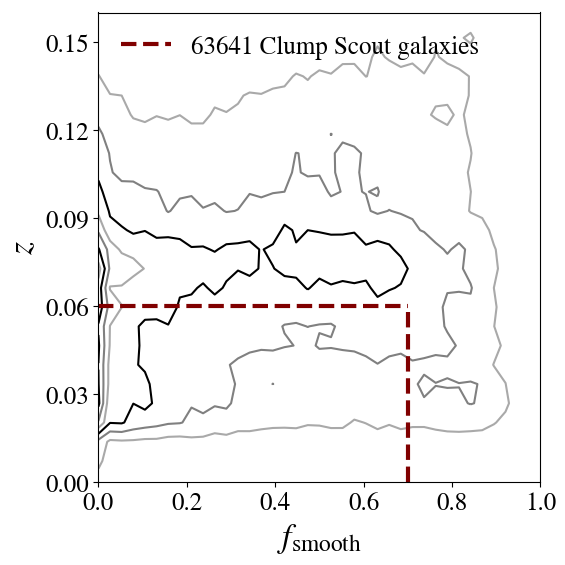
\includegraphics[width=5in]{Figures/clump_scout_sample_in_z-fsmooth.png}
\caption[\textit{Clump Scout} sample selection criteria from non-Stripe 82 GZ2 galaxy sample.]{\textit{Clump Scout} sample selection criteria from non-Stripe 82 GZ2 galaxy sample.}
\label{fig: clump scout sample}
\end{figure}



\subsection{Redshift evolution of \fclump}
With so many more clumpy galaxies at low redshift, we will be able to constrain clump origin formation theories. Specifically, we will investigate the evolution of the fraction of clumpy galaxies as a function of cosmic time, \fclump~(not to be confused with the GZH clumpy vote fraction). 

\cite{Guo2015} recently showed that the fraction of star-forming galaxies that have at least one off-center clump (\fclump) can be used to place constraints on theoretical models. By focusing on the redshift range between $0.5 <z<3$, they find that \fclump~changes with the stellar mass of the galaxies. Low-mass (M$<10$ 10 M) galaxies keep an almost constant fclumpy of $\sim$60\% from $z\sim3$ to $z\sim0.5$, while massive galaxies drop their \fclump~from 55\% at $z\sim3$ to 15\%, at $z\sim0.5$, as shown in Figure XXX \citep[adapted from][]{Guo2015}. \cite{Guo2015} argue that these observations support a model in which the clumpy star-formation results from multiple processes. In massive galaxies, the evolutionary trends are consistent with violent disk instability, however the apparent lack of \fclump~evolution in low mass galaxies is more consistent with a minor merger original. However, this conclusion, is based primarily on the lowest redshift bin probed by the \cite{Guo2015} data. In fact, when these data are combined with \fclump~measured from a variety of different surveys at $z<1$, the result is not so convincing anymore. The variation in the low-z measurements, however, is clearly large mostly as a consequence of non-uniform selection criteria and uncontrolled-for biases. \textit{Clump Scout} promises to provide the largest sample to date selected in a uniform fashion and with biases properly accounted for, especially in the low-mass regime where measurements of \fclump~can provide the strongest model constraints.

%In order to secure reliable measurements for \fclump~in the local universe, we must estimate the completeness of recovering low redshift clumpy galaxies from the SDSS sample. Ideally, we  To that end we need to conjure up some simulated clumpy galaxies that span the galactic mass and clump mass range appropriate for XXX reasons. 


\section{Summary and conclusions}
In this work, we have isolated a sample of galaxies with morphologies which resemble those of star-forming clumpy galaxies of the high-redshift universe. We identify these galaxies in the local universe through the Galaxy Zoo: Hubble project which included imaging from Stripe 82 of the SDSS. We isolate 105 galaxies that have a traditional clumpy morphology and acquire SDSS imaging and spectroscopic data for these galaxies, including spectra for over 150 clumps. We obtain stellar mass and star-formation rates for these galaxies through the GSWLC catalog. Through a preliminary analysis of the SDSS spectra we determine the clumps in these galaxies are in many ways consistent with high redshift clumps. However a more detailed analysis is necessary. 

Additionally, we describe the \textit{Clump Scout} project designed to search for additional clumpy galaxies in the local universe by presenting color-composite SDSS non-Stripe 82 imaging to the general public. We have made preliminary tests of this project with highly favorable reviews from volunteers and we expect to find an additional 1000 clumpy galaxies. This will provide a large statistical sample of local clumpy galaxies which will constrain the fraction of clumpy galaxies at low redshift allowing us to distinguish between various clump original theories. Additionally, because these are all SDSS objects, there will undoubtedly be spectra for thousands of clumps allowing for large statistical studies of star formation in the nearby universe. 

%Conclusion Chapter
%%%%%%%%%%%%%%%%%%%%%%%%%%%%%%%%%%%%%%%%%%%%%%%%%%%%%%%%%%%%%%%%%%%%
%!TEX root = thesis.tex
%%%%%%%%%%%%%%%%%%%%%%%%%%%%%%%%%%%%%%%%%%%%%%%%%%%%%%%%%%%%%%%%%%%%
\chapter{Summary \& Future Work}
\label{chap:summary}

The goal of this thesis was to develop a framework that brings both human and machine intelligence to the task of galaxy morphology to handle the scale and scope of next generation of astrophyical surveys. To this end we have measured traditional automated morphologies for $\sim$280K SDSS galaxies to use as features in a machine learning algorithm. We also utilized original Galaxy Zoo 2 volunteer classifications in various simulations in order to explore the impact of intelligent retirment of visual galaxy morphology classifications of a crowd-sourced project.  

Our simulations of Galaxy Zoo 2 classifications utilized 





We demonstrate nearly a factor of five increase in the classification rate, a reduction of
at least a factor of three in the human effort necessary to maintain that increased rate,
all while maintaining 95\% accuracy, nearly perfect completeness of ‘Featured’ subjects,
and with a purity that can be controlled by careful selection of input parameters to be
better than 90\% (see Appendix 3.4). Exploring those subjects wherein SWAP and GZ2
disagree, we conclude that the majority of this disagreement stems from the stochastic
nature of GZ2 raw labels. We now turn our focus towards incorporating a machine
classifier utilizing these SWAP-retired subjects as a training sample.

The goal of this thesis was to study the mass-loss histories of hypergiants stars using new capabilities in near-IR imaging and polarimetry, and airborne mid-IR imaging.  With LBT/LMIRCam and MMT-Pol on the MMT we have imaged the nebulae of VY CMa and IRC +10420 with sub-arcsecond resolution, revealing recent mass-loss in the close environments around these stars.  To probe further into these hypergiants' past history, we have used mid-infrared imaging with SOFIA/FORCAST to search for cold dust and performed 1-D radiative transfer modeling of their SEDs and resolved profiles.

Our 2 $-$ 5 $\micron$ adaptive optics imaging of the cool hypergiant VY CMa penetrates deeper into its dusty nebula than in the optical, probing its recent mass-loss history.  In Chapter 2 we analyzed the resolved images of its peculiar ``Southwest'' Clump, which has no obvious counterpart on the opposite side of the star.   The distinct shape of the SW Clump is suggestive of a short-lived, localized event and may be analogous to a coronal mass ejection (CME) from a single location on the Sun's surface.  A short-lived ejection event is consistent with the SW Clump appearing as a confined, coherent shape several hundred years after ejection.  Using adaptive optics imaging polarimetry, in Chapter 3 we demonstrated the Clump is optically thick through at least 3.1 $\micron$ and reaffirmed the lower limit mass of 5 $\times$ 10$^{-3}$ $M_{\sun}$ based on modeling its surface brightness as optically thick scattered light.  Our 1.3 $\micron$ polarimetry detects several other prominent features of VY CMa's nebula include the NW Arc, Arc 2, S Knot, and S Arc.  Using the polarized intensity as a lower limit on total scattered light intensity, we found each of these features to be optically thick as well.  Their relatively high intrinsic polarizations are consistent with their high scattering optical depths since the depolarizing effect of multiple scatters is reduced for typical silicate grain albedos.  In Chapter 4, we used 20 $-$ 37 $
\micron$ infrared imaging with SOFIA/FORCAST to search for evidence of earlier mass loss.  VY CMa's morphology at the longest wavelengths coincides with the general shape of the highly asymmetric nebulae seen in the visual, suggesting thermal emission from dust associated with the expanding arcs to the northwest and southwest.  Modeling its SED we computed an average mass-loss rate of 6 $\times$ 10$^{-4}$ $M_{\sun}$ yr$^{-1}$ over the past $\sim$1200 years, with no clear evidence of mass loss much farther in its past.

Our study of the warm hypergiant IRC +10420 similarly traced its mass-loss over a range of angular scales.  At the sub-arcsecond scale using adaptive optics, in Chapter 3 we used 2.2 $\micron$ polarimetry to reveal a relatively uniform nebula largely in the plane of the sky extending out to 2$\farcs$5 from the star.  This low-latitude ejecta is optically thick.  Combining the polarimetry with 3 $-$ 5 $\micron$ imaging that shows extended emission, we modeled the flux of this nebula and found its emission is an order of magnitude brighter than can be explained by simple extrapolation of the scattered light seen at $2.2~\micron$.  We hypothesized grains warmed to a temperature higher than the expected grain equilibrium temperature, but consistent with the local gas temperature in this region.  In Chapter 4 we presented 8 $-$ 12 $\micron$ adaptive optics images that reveal spatially extended emission spanning nearly the same range as the 2.2 $\micron$ polarimetry.  Applying radiative transfer modeling to the intensity profile of this extended emission and the SED, we found that IRC +10420's mass-loss history is divided into two distinct periods.  Our best-fit model showed that it lost mass at a high average rate of 2 $\times$ 10$^{-3}$ $M_{\sun}$ yr$^{-1}$ from 6000 $-$ 2000 yr ago during its presumed RSG stage, followed by an order of magnitude decrease to an average rate of 1 $\times$ 10$^{-4}$ $M_{\sun}$ yr$^{-1}$ in the past 2000 yr.

In addition to VY CMa and IRC +10420, our SOFIA/FORCAST program included the RSG $\mu$ Ceph and the warm hypergiant $\rho$ Cas.  Our study of $\mu$ Cep probes a mass-loss history extending back $\sim$13,000 yr.  To match the observed intensity profile of its resolved nebula in FORCAST 25 $-$ 37 $\micron$ images, our radiative transfer modeling requires a declining mass-loss rate.  We find that over the 13,000 yr dynamical age of the shell, its mass loss-rate has declined from 5 $\times$ 10$^{-6}$ to 1 $\times$ 10$^{-6}$ $M_{\sun}$ yr$^{-1}$.  In contrast to the high mass-loss rate of VY CMa, $\mu$ Cep's rate is significantly lower than RSGs of comparable luminosity.  In the case of $\rho$ Cas, we demonstrated that our new 19.7 $-$ 37.1 $\micron$ SOFIA/FORCAST photometry are consistent with the continued expansion and thinning of the dust shell formed as a result of the 1946 eruption.  We did not find evidence of new dust formation from more recent eruptions.

In the future, infrared imaging over a range of angular scales will be used to expand the sample of RSGs and post-RSGs with resolved mass-loss.  The SOFIA/FORCAST Cycle 3 program 03\_0082 (PI: R. Humphreys) included three additional RSG targets (NML Cyg, VX Sgr and S Per) and contingent approval has been granted for observations of the yellow hypergiant HR 5171A during a Cycle 4 Southern deployment if flight scheduling permits.  In Fall 2016, VY CMa is scheduled for observation with NOMIC, the 8 $-$ 13 $\micron$ imager on the Large Binocular Telescope.  With NOMIC's 0$\farcs$27 angular resolution (for single dish observing mode), VY CMa's SW Clump should be resolved.  These observations will better sample the Clump's SED and could help resolve the puzzle of its non-detection by ALMA reported in \citet{OGorman:2015}.  

The work presented in this thesis has demonstrated the capabilities of MMT-Pol and LMIRCam to resolve circumstellar ejecta around RSGs and post-RSGs.  These capabilities will be extended to several recently identified RSG clusters, each of which contains substantial coeval RSG populations.  These include RSGC1 \citep{Figer:2006,Davies:2008}, RSGC2 $=$ Stephenson 2 \citep{Davies:2007}, NGC 7419 \citep{Marco:2013} and the Per OB1 association, which contains many RSGs in its halo including S Per \citep{Humphreys:1978}.  Imaging these clusters of RSGs in polarized intensity in the near-infrared with MMT-Pol will cleanly separate light scattered by dusty nebulae from the stars' light, and when combined with adaptive optics imaging from 3 $-$ 13 $\micron$ with LMIRCam/NOMIC will enable us to trace the RSGs mass-loss.  Since the RSG cluster populations are coeval, this will allow the role of high mass loss events on their evolution to be studied.










% Bibliography
\bibliography{human-machine}  

% Appendices
\appendix
%!TEX root = thesis.tex


% APPENDIX
\chapter{Spectro-polarimetry Confirms Central Powering in a Ly$\alpha$ Nebula at z $= 3.09$} 
\label{app:LAB1}

\begin{quote}
\emph{A slightly modified version of this chapter has been published in The Astrophysical Journal with the following bibliographic reference:  Beck, Melanie; Scarlata, Claudia; Hayes, Matthew; Dijkstra, Mark; and Jones, Terry J. 2016, ApJ, 818, 138.}\\
\end{quote}

\begin{quote}
\begin{center}\textbf{Abstract}\end{center}
We present a follow-up study to the imaging polarimetry performed by \cite{HayesScarlata2011} on LAB1 in the SSA22 protocluster region. Arguably the most well-known Lyman-$\alpha$ ``blob", this radio-quiet emission-line nebula likely hosts a galaxy which is either undergoing significant star formation or hosts an AGN, or both. We obtain deep, spatially resolved spectro-polarimetry of the \lya~emission and detect integrated linear polarization of \textbf{$9$-$13\%\pm2$-$3\%$} at a distance of approximately 15 kpc north and south of the peak of the \lya~surface brightness with polarization vectors lying tangential to the galactic central source. In these same regions, we also detect a wavelength dependence in the polarization which is low at the center of the \lya~line profile and rises substantially in the wings of the profile. These polarization signatures are easily explained by a weak out-flowing shell model. The spectral dependence of the polarization presented here provide a framework for future observations and interpretations of the southern portion of LAB1 in that any model for this system must be able to reproduce this particular spectral dependence.
However, questions still remain for the northern-most spur of LAB1. In this region we detect total linear polarizatin of between 3 and 20\% at the 5\% significance level. Simulations predict that polarization should increase with radius for a symmetric geometry. That the northern spur does not suggests either that this region is not symmetric (which is likely) and exhibits variations in columns density, or that it is kinematically distinct from the rest of LAB1 and powered by another mechanism altogether.  
\end{quote}



\section{Introduction}\label{sec: intro}

First discovered over a decade ago during the course of deep optical narrowband imaging \citep{Francis1996, Steidel2000}, Lyman-$\alpha$ ``blobs" (LABs) are large, rare, gaseous nebulae in the high-redshift Universe detectable by their extensive \lya~luminosity.  Found predominantly in regions of galaxy overdensities \citep{Palunas2004, Matsuda2004, Prescott2008, Yang2009}, these objects are some of the most promising candidates for the study of ongoing galaxy formation \citep{Mori2006}.  Displaying a range of sizes from tens to hundreds of kiloparsecs and luminosities spanning $\sim10^{43-44}$ erg s$^{-1}$, LABs are reminiscent of high-redshift radio galaxies, yet most are not associated with strong radio sources \citep{Saito2006}. Instead, it seems that LABs are singularly associated with galaxies of one variety or another as even the famed Nilsson's Blob \citep{Nilsson2006}, widely cited as the most overt example of a host-less LAB,  is now believed to be associated with an AGN \citep{Prescott2015}. Other LABs have been associated with an assortment of galaxy populations including Lyman break galaxies (LBGs) \citep{Matsuda2004}, luminous infrared and submillimeter galaxies (SMGs) \citep{Geach2005, Geach2007, Yang2012}, unobscured and obscured quasars (QSOs) \citep{Bunker2003, Weidinger2004, Basu-Zych2004, Smith2009}, as well as starbursting galaxies \citep{Scarlata2009, Colbert2011}.  

Though most LABs seem to have in common a host galaxy or galaxies, the debate over the powering mechanism of the extended \lya~emission remains unresolved in part due to the fact that many of these galaxies seem unable to produce sufficient ionizing flux to light up the surrounding medium \citep{Matsuda2004, SmithJarvis2007}. In addition to photoionization from luminous AGN and/or young stars as a power source \citep{ HaimanRees2001, Jimenez2006, Geach2009, Cantalupo2012}, other possible mechanisms include mechanical energy injected by supernovae winds during powerful starbursts \citep{Taniguchi2000, Scarlata2009}, and radiative cooling \citep{Haiman2000, Fardal2001, DijkstraLoeb2009, Faucher-Giguere2010, Rosdahl2012}. In reality, it is more than likely that LABs are powered by multiple mechanisms simulataneously \citep{Furlanetto2005}. Theoretical studies have shown that polarization of  \lya~photons can be induced by scattering thus providing a potential diagnostic to probe these various powering mechanisms \citep{LeeAhn1998, RybickiLoeb1999, LoebRybicki1999, DijkstraLoeb2008}. 

In partiuclar, we focus our attention on a giant LAB (dubbed LAB1) in the SSA22 protocluster region first discovered by \cite{Steidel2000}.  This nebula is one of the most well-studied with observations ranging from optical to X-ray.  LAB1 is known to be loosely associated with an LBG \citep[C11,][]{Steidel2000, Matsuda2004},  though the peak \lya~surface brightness (SB) is more likely associated with an $850~\mu$m source \citep{Geach2014} with a weak radio counterpart \citep{Chapman2004} as well as associated detections in the near infrared \citep{Geach2007}, all suggestive of a dust-obscured star-forming galaxy leaking \lya~photons which interact with the surrounding medium. Deep integral-field spectroscopy of the \lya~emission has been presented by \citet{Weijmans2010} supporting this conclusion for the brightest regions of LAB1 though they suggest this mechanism is less promising in regions of lower \lya~SB. Additionally, \cite{McLinden2013} perform longslit NIR spectroscopy of portions of LAB1 detecting [OIII] emission in the LBGs C15 and C11 thus determining their systemic velocity.  
\citet[hereafter H11]{HayesScarlata2011} perform narrow-band imaging polarimetry and report low polarization in the central region rising to P=11.9$\pm$2\% within a radius of 7$''$ (45 kpc physical). Coupled with tangential polarization vectors around the central region, they conclude their observations are consistent with powering from an obscured galaxy resulting in scattered \lya~photons by HI.

Due to the observational expense involved, polarization measurements of spatially extended \lya~emission have so far been attempted only three times. In addition to the work of H11, \cite{Prescott2011} present narrow-band imaging polarimetry of a LAB associated with a radio-quiet galaxy at z=2.66 though polarization was not detected.  \cite{Humphrey2013} present the spectro-polarimetry of the gas surrounding the z=2.34 radio galaxy TXS 0211-122 and report low polarization centrally, rising to P=16.4$\pm$4.6\% in some parts of the nebula and conclude that at least a portion of the nebula is powered by the scattering of \lya ~photons produced by the galaxy within.  In this paper we present a follow-up to H11 with the first spectropolarimetric measurement of a radio-quiet LAB.  
In \S\ref{sec: theory} we discuss \lya~radiative transfer, scattering, and polarization basics. In \S\ref{sec: data} we discuss the observations and data analysis. Our methods and initial results are presented in \S\ref{sec: pol}, and in \S\ref{sec: interp} we present a discussion of our results in the context of recent observational work. Finally, in \S\ref{sec: future} we discuss the future of polarization as a diagnostic tool in relation to upcoming space-based polarimeters. 

%%%%%%%%%%% LYA RADIATIVE TRANSFER, SCATTERING AND POLARIZATION %%%%%%%%%%
\section{\lya~Polarization Basics}\label{sec: theory}
%%%%%%%%%%%%%%%%%%%%%%%%%%%%%%%%%%%%%%%%%%%%%%%%%%%%%%
\lya~polarization requires photons be scattered imbuing them with a preferential direction or impact angle. Localized (\textit{in situ}) production of \lya~photons, either from stars or gas, is not expected to have significant polarization as these photons will either not scatter sufficiently or have no preferential orientation. In this section we briefly review the necessary physics behind generating a significant \lya~polarization signal. 

The detection of signifiant polarization fraction of \lya~emission depends on two crucial factors: wing vs resonant scattering and Doppler boosting by thermal atoms in the surrounding medium. \lya~is the transition between the first excited and ground states of hydrogen and is a resonant transition, a doublet consisting of two fine-structure lines: $1S_{1/2} - 2P_{1/2}$ and $1S_{1/2}-2P_{3/2}$. The latter transistion can exhibit polarization while the former cannot as scattering through this transition does not retain information on the scattering angle thus producing an isotropized photon. Scattering ``near'' this doublet is called resonant or core scacttering and has been shown to be a superposition of Rayleigh and isotropic scattering producing a minimum level of polarization \citep{Brandt1959, Brasken1998}.  In most astrophysical circumstances \lya~undergoes this type of scattering and the \lya~photons are repeatedly absorbed and re-emitted until they are either destroyed by dust or escape the surrounding neutral medium. However, thermal motions within the gas cause  `partially' coherent scattering where the absorbed and emitted photons are equal only in the rest-frame of the scattering atom. To the outside observer, the \lya~photons  are Doppler boosted with respect to the scattering atom and thus perform a random walk in both frequency and physical space \citep{Neufeld1990, LoebRybicki1999}.  This can cause the \lya~photons to scatter in the wing of the profile where it has been shown that the phase function and degree of polarization are qualitatively consistent with pure Rayleigh scattering \citep{Stenflo1980}. Furthermore, \cite{Stenflo1980} has shown that wing scattering can produce three times more polarization than resonant scattering.  Thus, photons scattering in the wing of the profile are those which are most highly polarized and which see the lowest optical depth in the surrounding medium, enabling them to escape preferentially.

Theoretical predictions have been made by \cite{DijkstraLoeb2008} for the expected amount of polarization in the \lya~line for various astrophysical situations. They explore both an expanding shell and a collapsing cloud. The expanding shell is a simple model of backscattering off a galactic outflow and predicts polarization to increase with radial distance from the central source with total \lya~polarization as high as $40\%$, depending on the assumed column density and velocity of the outflow. Such large values of polarization can be understood due to the kinematics of the gas. Photons scattering off the ``back" of the expanding shell are quickly shifted out of resonance with the gas and into the wing of the line profile thus allowing many to escape after a single wing-scattering.  Similar levels of total polarization (\pol$\sim35\%$) are expected in the case of cooling radiation from a collapsing, optically thick gas cloud with the polarization again increasing as a function of radius from the central source due to photons emitted over a spatially extended region within the cloud. . 

In both cases, detecting a high level of polarization through narrow-band imaging polarimetry would be able to rule out \textit{in situ} production of \lya~photons. However, imaging polarimetry alone can not distinguish between outflows or inflows as both predict similar levels of polarization and increasing polarization as a function of radius from the central source. Instead, the frequency dependence of \lya~polarization is required. For the case of an outflowing thin shell, \cite{DijkstraLoeb2008} predict that \lya~polarization will increase redwards of the line center. This is because the redder \lya~photons appear farther from resonance in the frame of the gas and scatter less thus achieving higher levels of polarization. In fact, \cite{DijkstraLoeb2008} state that this frequency dependence can be interpreted as a ``fingerprint" for outflows and predict that \lya~polarization could be as high as $\sim60\%$ in the reddest part of the line profile.  In stark contrast, polarization  increases blueward of line center for a collapsing cloud. Thus the frequency dependence of \lya~polarization can also constrain the kinematic structure of the surrounding gas.

% ------------------------------------------------ SPECTROPOLARIMETRY ------------------------------------------------------
\section{Observations, Reduction, and Calculations}\label{sec: data}
We now turn our attention to the spectro-polarimetry of LAB1.  \cite{HayesScarlata2011} present imaging polarimetry of this nebula in which they find significant polarization increasing as a function of radius from the point of brightest \lya~SB as calculated in Voronoi bins. Furthermore they find polarization vectors which lie tangentially around this central point and conclude that LAB1 is indeed powered by a bright central galaxy obscured from our line of sight. In this portion of the paper we present follow-up spectro-polarimetry in order to confirm and further probe the kinematics of this enigmatic object. In this section we discuss the observations and data reduction methods, as well as the polarization and error calculations performed.

\subsection{Observations}
We choose as our target one of the largest known \lya~blobs located in the SSA22 protocluster region at z=3.09 (see \cite{Steidel2000}).  Dubbed LAB1, this object was observed over the course of five consecutive half nights from 5-9 October 2010, using the FOcal Reducer and low dispersion Spectrograph (FORS2) \citep{Appenzeller1998} instrument mounted on the Antu (UT1) node of the Very Large Telescope (VLT) European Southern Observatory (ESO). The first stage of the dedicated dual-beam polarization optics is the introduction of a strip mask designed to avoid overlapping on the CCD of the two beams of polarized light.  Six MOS slitlets, each 1$''$ wide and 20$''$ long are then positioned over the objects of interest. The light is passed through a super-achromatic half-wave plate (HWP) retarder mosaic (\texttt{RETA2+5}), which rotates the angle of the polarized light. We adopt the standard four angles for unambiguous recovery of the Q and U Stokes parameters: 0\degs, 22.5\degs, 45\degs, and 67.5\degs. The rotated beam is subsequently passed through a Wollaston prism (\texttt{WOLL\_34+13}), which splits the randomly polarized and unpolarized light into two orthogonal, linearly polarized outgoing beams, arbritrarily denoted  the `ordinary' (\ord) and `extraordinary' (\ext) beams. Finally, the beams are passed through a grism dispersion element  (\texttt{GRISM\_1400V+18}) with a central wavelength of 5200 \AA~($\sim$1271 \AA~rest frame), spectral range of 4560-5860~\AA, and dispersion of .63 \AA/pixel. The spectral resolution is approximately 2100 with our 1$''$ slit width. This produces simultaneous \ord~and \ext~spectra which are then projected onto the CCD. Thus each frame consisted of six spectra: three slits contained only sky, two contained stars which were used in the alignment process (see below), and one was positioned over LAB1. We observed LAB1 at a position angle of $-3.09$\degs~in the standard N=0\degs -- E=90\degs~reference frame. 

Throughout the course of each night the sequence of four HWP position angles was observed repeatedly with two full sequences being completed each night. Integration times were 1,800 seconds for each HWP position with the exception of the first night where each exposure had 1,600 and 2,000 seconds of integration time per HWP position for the first and second sequences respectively. Thus at each retarder position angle we obtain a total integration time of 18,000 seconds. 

The entirety of the observing time was classified as clear or photometric with no clouds present on any given night. Since the \ord~and \ext~beams are obtained simultaneously, deviations from photometricity would anyway have no impact on the determination of the Stokes parameters. Observations were taken around the new moon in order to minimize the sky background at bluer wavelengths with moonrise not occurring until after observations were complete each night. Because we observe LAB1 with constant position angle, atmospheric dispersion will vary with airmass over the course of the exposure time. Airmass ranged from 1.1 to 1.53 and was thus well within the FORS instrument's atmospheric dispersion corrector to compensate.  The bulk of the 20 hours of observation time experienced astronomical seeing which varied between 0.5 and 1.0 arcsecond with median seeing at $\sim0.''75$. There were three observations which experienced seeing as high as $1.7''$. These were excluded from the following analysis although their inclusion does not significantly alter our results -- polarization fractions varied only by a few per cent. We thus obtain a total of 37 individual observations for a total of 12,600 seconds of integration.  

% TOTAL INTENSITY FIGURE
\begin{figure}
\begin{center}
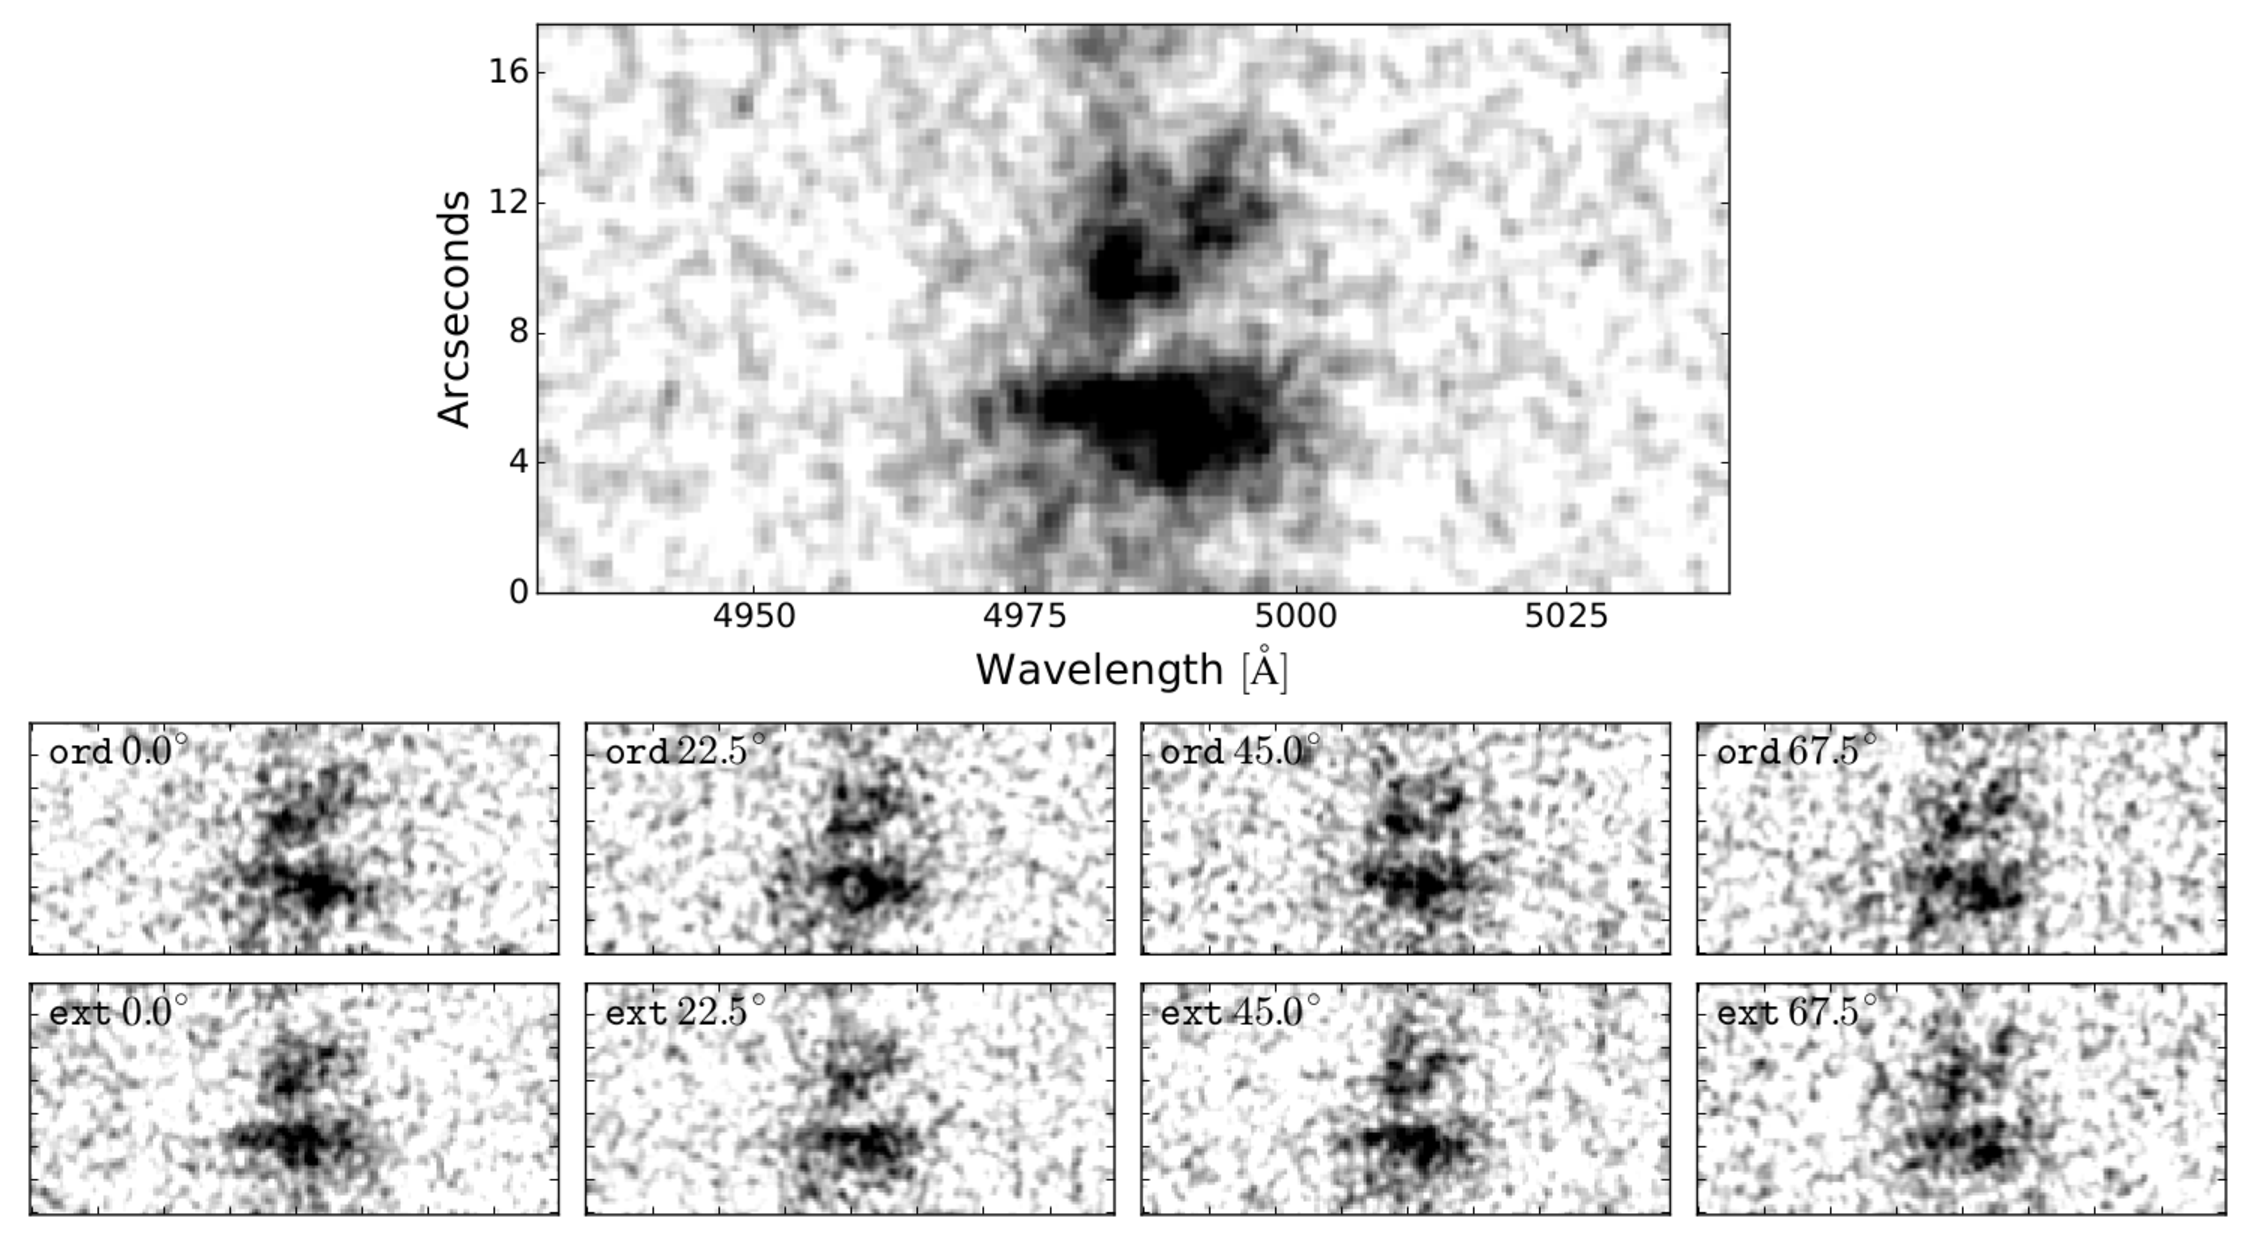
\includegraphics[width=\linewidth]{Figures/lyapol/f1_f7_combo.pdf}
\caption[Science frames for \lya~polarimetry of LAB1]{\emph{Top.} Spatial and wavelength distribution of the master total intensity \lya~spectrum. Co-added \lya~spectrum of 77 science spectra smoothed by a Gaussian with FWHM = 0\farcs5. Due to light loss at the edges of the slit, we present here only the central $18''$. \emph{Bottom.} Ordinary and extraordinary beams at each HWP angle which provide the basis for our polarization measurements. Each frame consists of several co-added frames taken over the 5 nights of observations.}
\label{fig: scienceframes and totint}
\end{center}
\end{figure}

%%%%%%%%%%%%%%%%%%%%%%%%%%%%%%%%%%%%%%%%%%%%%%%%%%%%%%%
% 	Data Reduction
%%%%%%%%%%%%%%%%%%%%%%%%%%%%%%%%%%%%%%%%%%%%%%%%%%%%%%%

\subsection{Data Reduction}\label{sec: dataredux}

% SLIT POSITION FIGURE
\begin{figure*}
\begin{center}
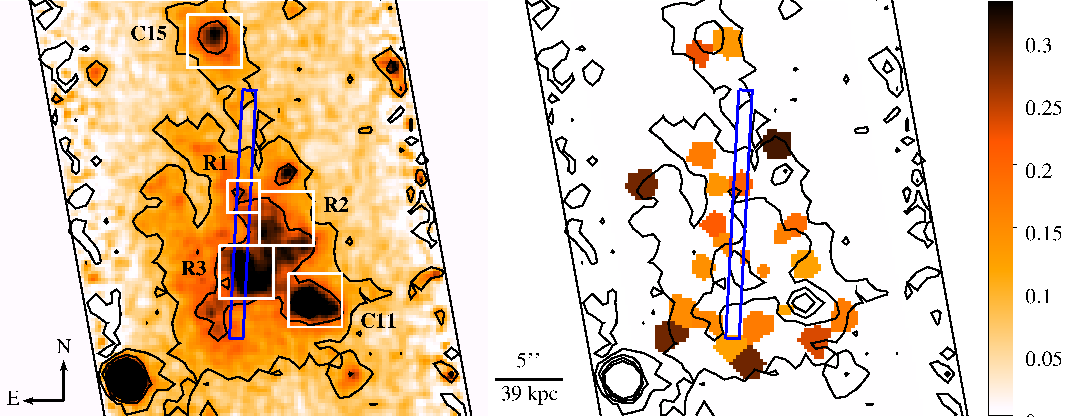
\includegraphics[width=\linewidth]{Figures/lyapol/f2_v2.pdf}
\caption[Slit position over LAB1 as compared with results from Hayes et. 2011]{Slit position over LAB1 as compared with results from H11. In the left panel we show the combined \lya~intensity frame from H11 adaptively smoothed to show detail including emission from LAB1 and nearby LBGs C11 and C15. Overlaid in white are boxes from \cite{Weijmans2010}, regions in which they performed integral-field spectroscopy on the \lya~emission. As before, the slit shown here spans $\sim$18$''$.  Contours denote arbitrary flux levels. In the right panel we show fractional polarization results from H11 for those bins which were detected at or above 2$\sigma$ (See H11 Fig. 2, panel \textbf{e}). Our slit passes over the region of brightest \lya~emission in the southern portion of the slit as well as a dimmer region in the north.}
\label{fig: slit}
\end{center}
\end{figure*}

The intial steps of data reduction were carried out in the standard manner for spectroscopic observations. Individual frames were biased subtracted. Master flat frames were created from several dome flats using EsoRex\footnote{\url{http://www.eso.org/sci/software/cpl/esorex.html}}, an ESO recipe execution tool, and applied to individual frames to correct for pixel-to-pixel variations. Each frame was then normalized by exposure time. Cosmic rays were throroughly removed using L.A. Cosmic\footnote{\url{http://www.astro.yale.edu/dokkum/lacosmic/}} \citep{vanDokkum2001}. To account for small variations in the spatial direction during observing, frames were aligned using the \texttt{shift\_sub} function in IDL where the pixel shift was calculated as the average of fitted Gaussians of each stellar continua in the slits above and below the science spectra.   At this stage all the individual frames were split into their \ord~and \ext~beams (37 observations $\times$ 2 beams = 74 spectra). Only slits 3 (sky) and 4 (LAB1) were considered for the remainder of the analysis. 

Each beam of the sky and LAB1 spectra was wavelength calibrated individually via a He-Ar arc lamp spectrum using \texttt{NOAO/IRAF}\footnote{IRAF is distributed by the National Optical Astronomy Observatories, which are operated by the Association of Universities for Research in Astronomy, Inc., under cooperative agreement with the National Science Foundation} \texttt{onedspec} and \texttt{twodspec} packages. The \texttt{identify - reidentify - fitcoords - transform} sequence was used on the 2D spectra yielding a fit r.m.s. typically between 0.05 and 0.09 \AA.


Sky subtraction was performed using the sky spectra in slit 3. For each \ord~and \ext~beam, the sky spectrum was median extracted, normalized to the spatial dimension of the 2D LAB1 spectra, and subtracted from the corresponding LAB1 beam.  The residual sky background in the wavelength direction was modeled with a linear fit after masking the \lya~line. This was then subtracted from the spectra. This step was appropriate as there is no evidence of UV continuum according to our preliminary analysis of recently acquired MUSE data which will be published in Hayes et al., in prep. Atmospheric correction was applied using an extinction coefficient as a function of wavelength obtained from \cite{Patat2011} and the airmass at the midpoint of each observation. Spectra were then co-added using a mean combination with simple \texttt{minmax} rejection of the highest and lowest value at each pixel using IRAF's \texttt{imcombine}. As mentioned previously, we exclude 3 observations from further analysis. These include one 45\degs~observation and two 67.5\degs~observations whose delivered seeing was well above $1.0''$. 

We combine eight groups of 10 spectra to produce science frames for polarimetry measurements: \ord~and \ext~at each of the four angles, as shown in the bottom panel of \autoref{fig: scienceframes and totint}. It is immediately obvious that there are variations between the \ord~and \ext~beams at each HWP angle which fundamentally leads to a measurement of the polarization.  Finally, a master total intensity frame is created by averaging these eight frames together, as shown in the top panel of \autoref{fig: scienceframes and totint}.
 


%%%%%%%%%%%%%%%%%%%%%%%%%%%%%%%%%%%%%%%%%%%%%%%%%%%%%%%
% 	Polarization Calculations
%%%%%%%%%%%%%%%%%%%%%%%%%%%%%%%%%%%%%%%%%%%%%%%%%%%%%%%
\subsection{Polarization and Error Calculations}\label{sec:analysis}
Polarization of \lya~is expected to be linear, thus the decomposition of polarized light falls only into $Q$ and $U$ normalized Stokes parameters. The $V$ parameter represents circular polarization and is not expected for \lya ~radiation. The fourth parameter $I$ is the total intensity which is equal to the sum of the \ord~and \ext~beams.  For each HWP position, $\theta$, the normalized flux difference, $F_{\theta}$, is defined as:

\begin{equation}\label{eqn:normflux}
F_{\theta}=\frac{f_{\theta}^{ord} - f_{\theta}^{ext} }{f_{\theta}^{ord} + f_{\theta}^{ext}}
\end{equation}
where $f^{ord}_{\theta}$ is the flux in the ordinary beam for a given $\theta$ and likewise of $f^{ext}_{\theta}$ for the extraordinary beam.
 
Once the four HWP angles have been obtained, $Q$, $U$, and $I$ relate to the observables by
\begin{equation}
\begin{aligned}
&q = \frac{Q}{I}= \frac{1}{2}F_{0.0} - \frac{1}{2}F_{45.0} \\
&u = \frac{U}{I}= \frac{1}{2}F_{22.5} - \frac{1}{2}F_{67.5}
\end{aligned}\label{eqn:stokes}
\end{equation}
From these, the polarization fraction, \pol, and the polarization angle, $\chi$, can be calculated by
\begin{equation}
\begin{aligned}
&p = \sqrt{q^2 + u^2} \\
&\chi = \frac{1}{2} \arctan{\frac{u}{q}}
\end{aligned}\label{eqn:pol-angle}
\end{equation}

However, we actually desire an estimate of the ``true'' polarization,  \po.  When it is assumed that the Stokes parameters $q$ and $u$ are drawn from Gaussian distributions centered around the true values ($q_0$ and $u_0$) each with variance $\sigma$,  it can be shown \cite[e.g.][]{Plaszczynski2014} that the distribution of the polarization follows the Rice distribution:
\begin{equation}
f_p(p) = \frac{p}{\sigma^2}\mathrm{e}^{-\frac{p^2 + p_0^2}{2\sigma^2}}I_0(\frac{pp_0}{\sigma^2})
\end{equation}
where $p_0$ is the true amplitude of the polarization and $I_0$ is the modified Bessel function of the zeroth order.  \autoref{eqn:pol-angle} is considered the naive estimator for this distribution and is known to be strongly biased at low polarization signal-to-noise ratio (SNR$_p$) in part because, in this regime, the Rice distribution can be approximated as a Rayleigh distribution which is highly skewed to larger values of polarization. Additionally, the naive estimator cannot take experimental noise into account. Several attempts have been made to produce an unbiased estimator for \po~\citep[see][for a review]{SimmonsStewart1985} but most have other undesirable qualities such as being unphysical at very low signal-to-noise or containing discontinuities.  \cite{Plaszczynski2014} develop a polarization estimator dubbed the Modifed Asymptotic Estimator (MAS) which is less biased in both low (Rayleigh) and high (Gaussian) SNR$_p$ regimes and is continuous between these regions. Furthermore, this estimator also takes into account measurement error in $q$ and $u$. For these reasons we adopt this estimator for the polarization which goes as:
\begin{equation}\label{eqn: pmas}
\hat{p}_{MAS} = p_i - b_i^2\frac{1-\exp^{-p_i^2/b_i^2}}{2p_i}
\end{equation}
where $p_i$ is given by \autoref{eqn:pol-angle} and $b^2$ is the noise bias of the estimator given by
\begin{equation}\label{eqn: noisebias}
b_i^2 = \frac{q_i^2\sigma_u^2 + u_i^2\sigma_q^2}{q_i^2 + u_i^2}
\end{equation}
where each $i$ is an individual binned measurement of the quantity of interest.

In practice, the quantities $p_i$, $q_i$ and $u_i$ are calculated as given in equations   \ref{eqn:normflux}, \ref{eqn:stokes}, and~\ref{eqn:pol-angle} in each bin (see below for a discussion on our binning strategy).  The $\sigma_q$ and $\sigma_u$ are computed from Monte Carlo simulations whereby each of the eight science frames is allowed to deviate according to a Gaussian spread wherein the deviates are simply computed as the standard deviation of a large portion of the background of each individual science \ord~and \ext~frame. Ten thousand realizations are performed and for each realization $q$ and $u$ are computed. The resulting probability distributions of $q$ and $u$ are Gaussian as expected and from these we obtain $\sigma_q$ and $\sigma_u$ by measuring the spread of the distributions.

We consider the polarization SNR$_p$ by computing 
\begin{equation}\label{eqn: snr}
SNR_p = \frac{p_{MAS}}{\sqrt{\frac{1}{2}(\sigma_q^2 + \sigma_u^2)}},
\end{equation}
where again we allow for measurement error by incorporating both $\sigma_q$ and $\sigma_u$.
Following the prescription of \cite{Plaszczynski2014}, values of SNR$_p > 3.8$ indicate that the Rice distribution is sufficiently Gaussian and thus unbiased. In this regime one may compute a point estimate along with the estimator variance. Values less than this, however, fall in the Rayleigh regime wherein one must instead rely on confidence intervals (CIs).  As we show below, different binning techniques yield different SNR$_p$ and thus in some cases we report point estimates of the fractional polarization while in others we provide the 95\% CIs according to Eqn.~26 in \cite{Plaszczynski2014}.

Finally, we consider the measurement and error estimates for the polarization angle. It has been shown \cite[e.g.][]{WardleKronberg1974, Vinokur1965} that the distribution of $\chi$ is symmetric about the true value of the angle and thus the estimator presented in \autoref{eqn:pol-angle} is already unbiased. At large SNR$_p$ this distribution also tends towards a Gaussian with a standard deviation of  $\sigma_{\chi} \approx \sigma_p/2p$. However, at low SNR$_p$ this approximation underestimates the error. In this work we follow \cite{WardleKronberg1974} and approximate the error by their Eqn.~A6 (see also their Figure 3) which provides the most conservative error estimate for measurements with SNR$_p > 0.5$.

%-------------------------------------------------------figures-----------------------------------------------------------------------
% Integrated Polarization - BIG BOXES
\begin{figure*}
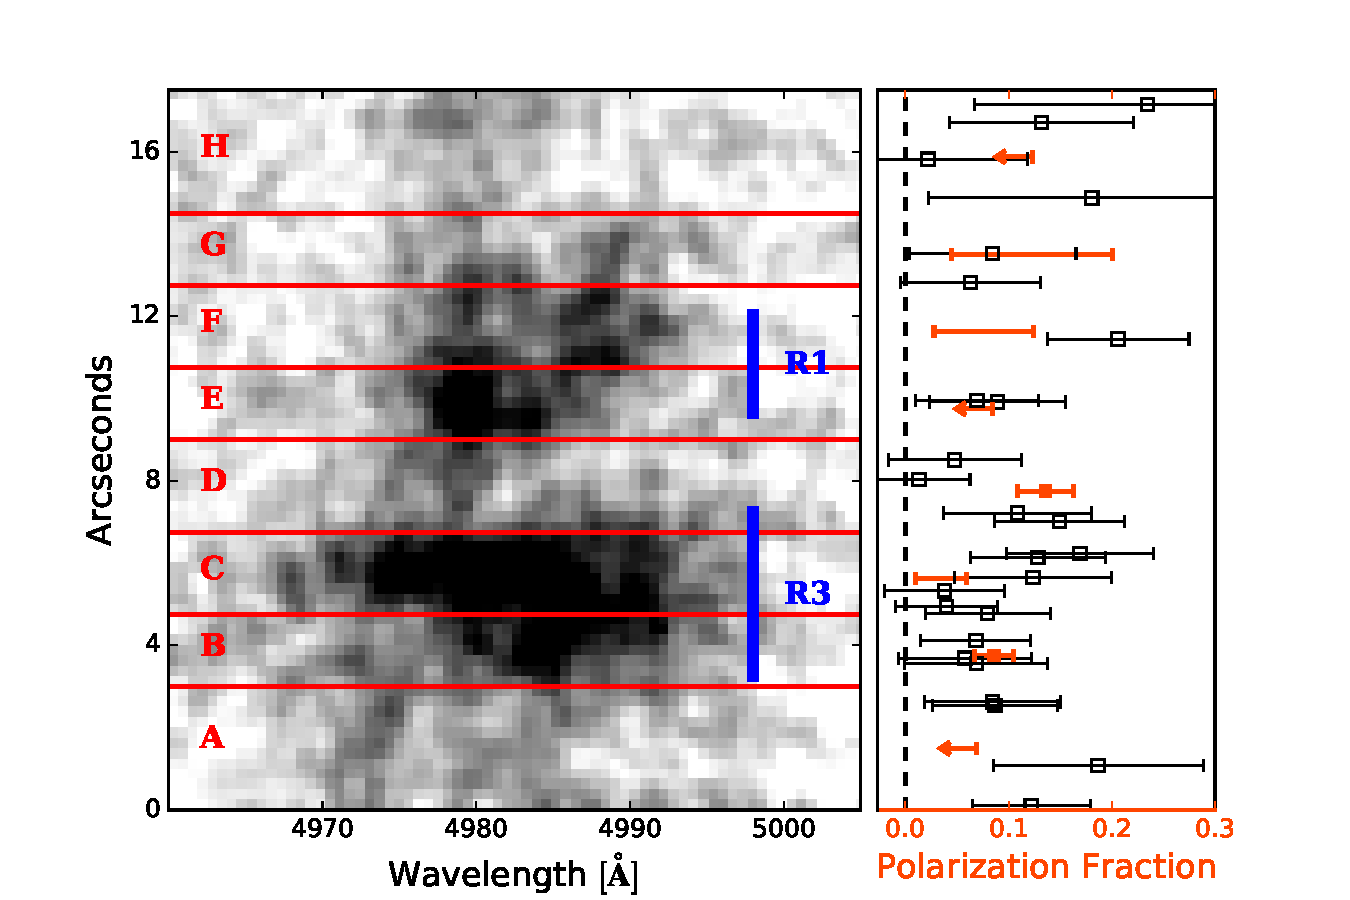
\includegraphics[width=\linewidth]{Figures/lyapol/f3_v2.pdf}
\caption[Polarization of spectrally integrated \lya]{Polarization of spectrally integrated \lya. In the left panel we show the spatial binning of the \lya~emission spectrum with bins ranging from 2-3$''$ overlaid in red.  \lya~emission is integrated over 4965-5000~\AA. The blue lines indicate the spatial extent of \cite{Weijmans2010} IFU boxes.  Depicted in the right panel are our polarization measurements in orange.  Polarization point estimates are denoted by orange boxes with $1 \sigma$ error bars;  95\% CIs are shown as closed brackets; and upper limits are denoted with orange arrows where we define our upper limits as the upper 95\% confidence bound for that spatial bin. Black squares show fractional polarization from H11 as measured in Voronoi bins which overlap with our slit. See text for discussion on differences and limitations between datasets.}
\label{fig: totpol}
\end{figure*}

%-------------------------------------------------------figures-----------------------------------------------------------------------


%%%%%%%%%%%%%%%%%%%%%%%%%%%%%%%%%%%%%%%%%%%%%%%%%%%%%%%
% 	POLARIZATION OF LAB1
%%%%%%%%%%%%%%%%%%%%%%%%%%%%%%%%%%%%%%%%%%%%%%%%%%%%%%
\section{Polarization of \lya~in LAB1}\label{sec: pol}
\subsection{Polarization integrated over the line profile}\label{sec: spatial pol}

Because our data have low signal-to-noise per pixel (SNR$_p \lesssim 1$), binning of the science frames is a necessity. However, any \lya~polarization signal will result from the particular geometry inherent in the HI gas with a unique set of Stokes parameters and polarization angle. If these regions are not azimuthally resolved, one risks overlapping each region's polarization angles thus averaging the polarization signal and potentially washing it out entirely~\citep{DijkstraLoeb2008}. Thus, some binning is necessary but overbinning will make it unmeasurable. 


To aid in the determination of appropriate bins we examine the slit position over LAB1 as shown in \autoref{fig: slit}.  LAB1 fills the slit and contains regions of varying \lya~surface brightness (SB) as denoted by the set of arbitrary contours. Also shown in this figure are white boxes corresponding to \lya~emission integral-field spectroscopy as presented by \cite{Weijmans2010}. Our slit overlaps their regions \textbf{R1} and \textbf{R3} and we adopt this nomenclature throughout. \textbf{R3} is situated over the brightest peak of the \lya~SB while \textbf{R1} is associated with a somewhat dimmer region. Between these two features there exists a distinct gap that can also clearly be seen in the \lya~emission shown in \autoref{fig: scienceframes and totint}. We determine to bin these regions separately as they can exhibit different polarization fractions as shown in the right panel of \autoref{fig: slit}. Altogether, we bin the slit into 8 individual spatial regions, each spanning $2''$--$3''$, as this is large enough to achieve adequate SNR$_p$ in some bins yet small enough that we do not wash out any polarization signal. These spatial elements are labelled \textbf{A} through \textbf{H},  with \textbf{A} being the southern-most portion of the slit and \textbf{H} the northern-most. These spatial bins are shown explicitly in \autoref{fig: totpol}.

%\capstartfalse
\begin{table}
	\begin{center}
	\caption[Polarization signal-to-noise and fractional polarization for spatial binning of LAB1]{\sf{Polarization signal-to-noise and fractional polarization measurements for spatial bins. For those bins with sufficient SNR$_p$ we report the polarization point estimate and corresonding $1 \sigma_p$ error. Otherwise we report 95\% confidence intervals for bins in which the lower 95\% confidence bound is greater than zero.}}
	\resizebox{.48\textwidth}{!}{
 		\begin{tabular}{l c c c c c}
		\hline
		Bin & SNR$_p$ &  $p_{min}$ & $p_{max}$ & $p$ & $\sigma_p$  \\
		\hline
		\hline
		B &  4.6 &  &  & 8.59 & 1.9\\
		C &  2.6 & 1.00 & 5.92  \\
		D & 4.9  &  &  & 13.6 &  2.7 \\
		F &  2.8  & 2.78 & 12.4 &   \\
		G & 2.8  & 4.51 & 20.0 &  \\
		\hline 
		\end{tabular} }
	\end{center}

	\label{table: bigboxCLs}
\end{table}
%\capstarttrue

\begin{figure}
\begin{center}
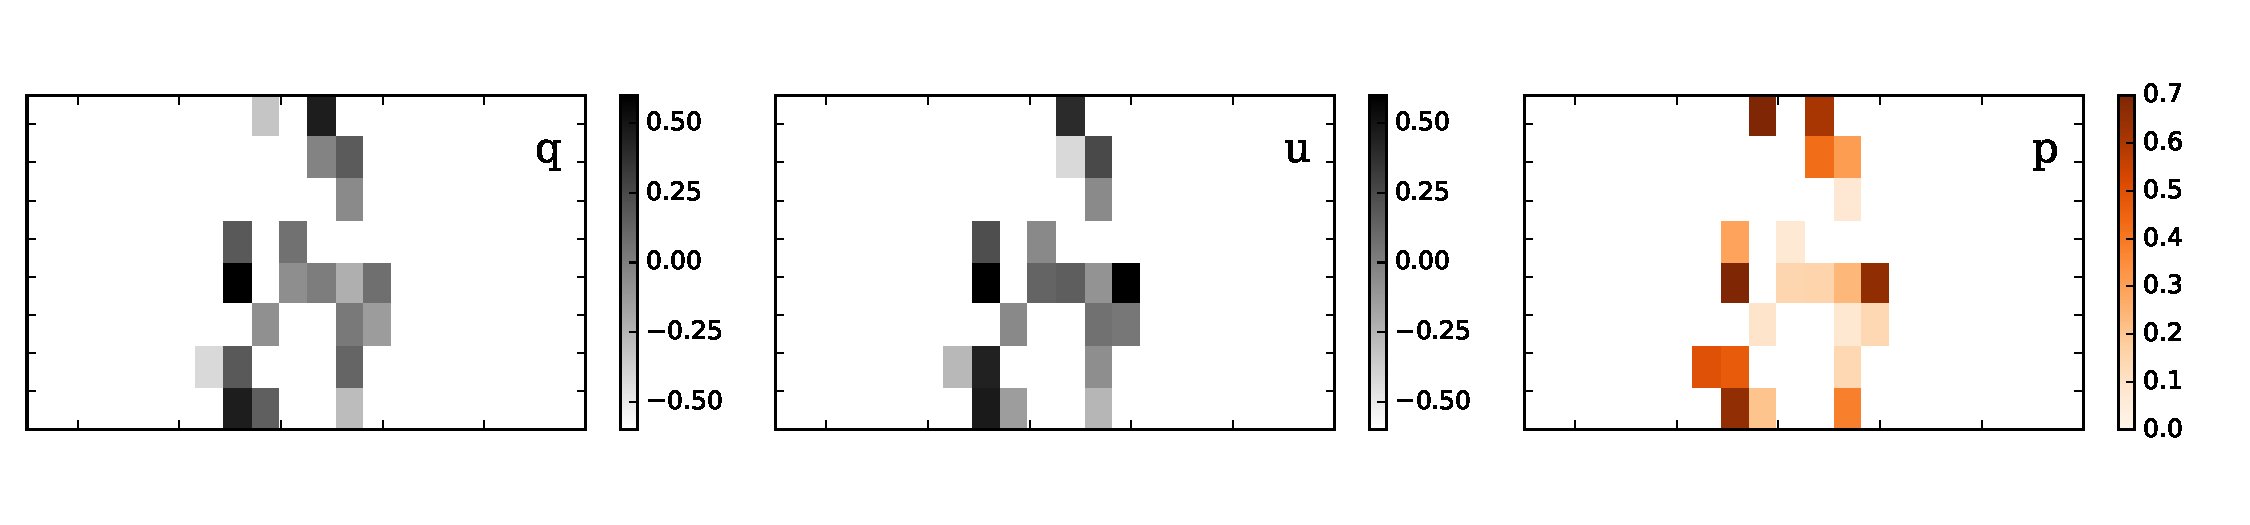
\includegraphics[width=\linewidth]{Figures/lyapol/f8_v2.pdf}
\caption[2D Stokes parameters and polarization map of LAB1]{2D Stokes parameters and polarization maps. The $q$ and $u$ maps are computed directly from the science frames shown in the bottom panel of \autoref{fig: scienceframes and totint} according to the prescription of \autoref{eqn:stokes} after binning as described in \autoref{sec: wavelength pol}. The polarization map in the right panel is then computed via $q$ and $u$ according to \autoref{eqn: pmas}. In all frames, only those bins are shown in which the polarization was deemed significant as discussed in \autoref{sec:analysis}. The variation between the $q$ and $u$ maps is readily seen by eye and is directly related to the amplitude of the polarization measured in that bin.}
\label{fig: QU}
\end{center}
\end{figure}

With these considerations in mind we first spectrally integrate over the \lya~emission to calculate the total \pol~for comparison with H11.  Integration is carried out over the wavelength range 4965--5000~\AA. We note that though the range of the \lya~emission varies within each aperture, varying the integration range only changes the fractional polarization by a few percent difference for all but bin \textbf{H} which has an increase in \pol~of $10\%$. However, since we are unable to place reasonable constraints on the polarization fraction in this bin we  consider this to be moot. Only two of these spatial bins have SNR$_p > 3.8$ and for these we report the measured polarization and $1\sigma_p$ error.  The remaining bins have SNR$_p < 3.8$ and for these we report 95\% CIs for those bins in which the 95\% lower confidence bound is greater than zero. Our results are summarized in Table 1 as well as in \autoref{fig: totpol} along with the spatial binning pattern and the polarization measurements from H11 for those bins which our slit overlapped. The fractional polarization values roughly agree when one takes into account the distinct methods used between our two analyses. H11 utilize a Voronoi binning technique whereby the size of each bin is determined by the achieved SNR within that bin. This allows them to have bins of various sizes. Each of their bins only partially overlaps our slit and we include in \autoref{fig: totpol} all such bins. The largest disparity between datasets occurs in Bin F. In this region, H11 measure the fractional polarization to be $p\sim20\%$ whereas we find, at most, $\sim12\%$. The reason for this discrepancy is not fully understood. In \autoref{table: bigboxCLs} we report the 95\% confidence intervals for those spatial bins whose lower 95\% confidence bound is greater than zero. We see polarization in spatial bin \textbf{C} which is on the order of a few per-cent though not quite consistent with zero. The fractional polarization then increases to 13.6\% north and 8.6\% south of this region as seen in spatial bins \textbf{B} and \textbf{D}. The distance between bin \textbf{C} and these bins is roughly 15 kpc in either direction. 


% 1D POLARIZATION AND LINE PROFILES
\begin{figure}
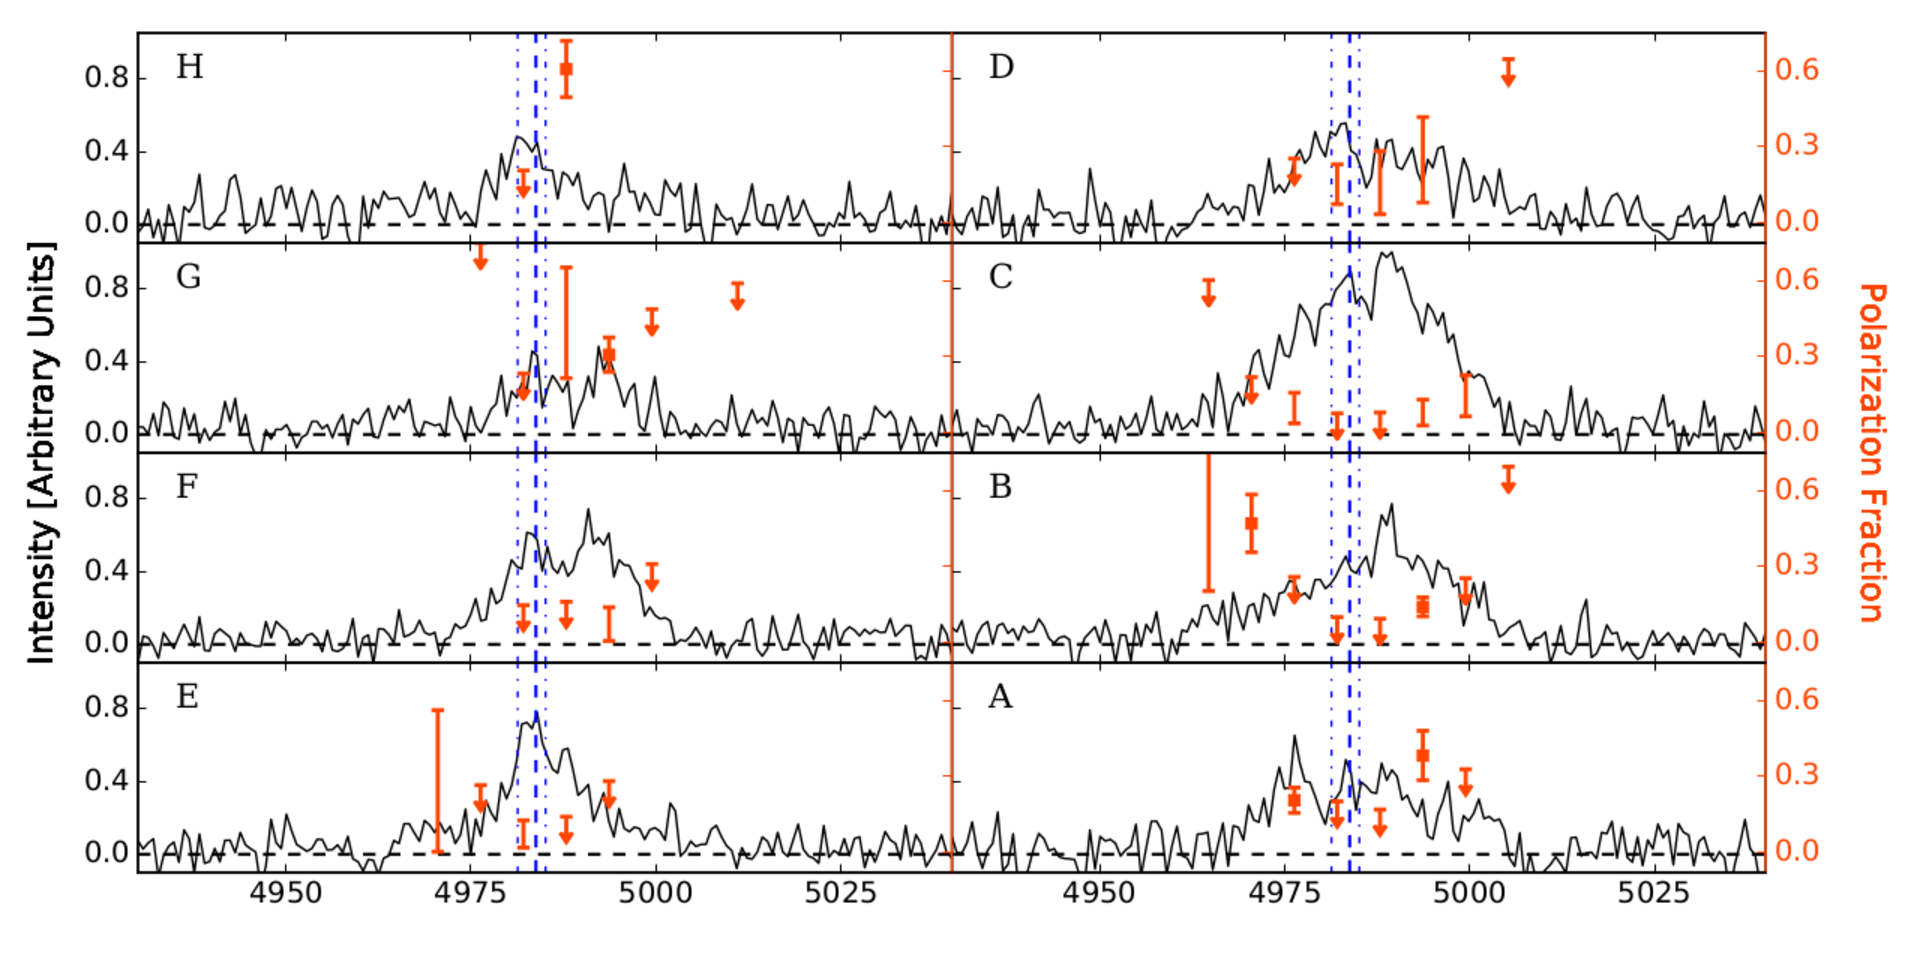
\includegraphics[width=\linewidth]{Figures/lyapol/f4_v2.pdf}
\caption[Polarization as a function of wavelength for each spatial bin]{Polarization of \lya~as a function of wavelength. Figures \textbf{A} through \textbf{H} contain the extracted 1D \lya~spectrum of the corresponding aperture from \autoref{fig: totpol}. All spectra have been scaled to show their relative intensity. Overplotted in orange we show the polarization fraction as a function of wavelength in bins of 5\AA.  Polarization point estimates are denoted by orange boxes with $1 \sigma$ error bars;  95\% CIs are shown as closed brackets; and upper limits are denoted with orange arrows where we define our upper limits as the upper 95\% confidence bound for that bin. The dashed blue line represents the average systemic velocity as measured from \oiii of four galaxies which are associated with LAB1. The dash-dotted lines are the minimum and maximum of those objects. In bins \textbf{B}-\textbf{E},  we see a trend of low polarization associated with the core of the \lya~emission and higher polarization toward the wings of the line profile. This trend is less apparent in other bins, though the line profiles are not as well defined and many display a double peak. In general, \pol~is typically highest at those wavelengths in which the \lya~intensity is relatively low.}
\label{fig: oned}
\end{figure}


\subsection{Polarization across the line profile}\label{sec: wavelength pol}
We next explore \pol~as a function of wavelength. Using the same spatial elements, we further bin each into 5~\AA~increments in the wavelength direction and compute $q$ and $u$ as shown in \autoref{fig: QU}. In this figure we show only those bins in which we that we detect a significant polarization signal. One can see by eye the differences in the $q$ and $u$ frames which is directly responsible for the strength of the polarization shown in the third panel. 

In \autoref{fig: oned} we present the extracted 1D spectra for each spatial element along with the wavelength response of \pol~in orange.  For those bins with sufficient SNR$_p$ (as shown in the middle panel of \autoref{fig: pol2d}), we show the polarization point estimate along with $1 \sigma_p$ errors. For those bins which have lower 95\% confidence bounds greater than zero, we show the CI as orange closed brackets. Otherwise, we show upper limits defined as the upper 95\% confidence bound for that bin. In general we see a trend of high (low) polarization corresponding to lower (higher) relative \lya~intensity. In particular, bin \textbf{B}  displays \pol~which is consistent with zero in near 4985\AA~but which rises substantially in the wings of the profile, reaching up to $45\%$ bluewards and with upper limits as high as $65\%$ redwards.  In spatial bins \textbf{C} and \textbf{D} we see the suggestion of similar behavior with lower polarization in the core of the line and potentially higher polarization in the wings of the profile though the data do not allow us to furher constrain the trend. 

It is important to recall that these measurements inform us as to the fraction of the total intensity which is polarized. In the case of box \textbf{B}, for example, the wavelength bin at 4970\AA~is 45\% polarized. The intensity in this portion of the line is quite low, however, relative to the peak at 4990\AA. It is instructive to compare this to the integrated polarization in \autoref{fig: totpol}. In that figure, box \textbf{B} has fractional polarization of $\sim9\%$. Thus we see that spectropolarimetry gives us more information than what can be gained solely through imaging or integrated polarimetry. Highly polarized individual wavelength bins are `washed out' by the relative strength of the core of the profile which is typically not strongly polarized. The overall fraction of polarized photons decreases when integrating over the entire line and it is impossible to reconstruct from imaging alone which wavelength regimes are the most highly polarized.

% 2D POLARIZATION FIGURE - RECT BINS
\begin{figure}
\begin{center}
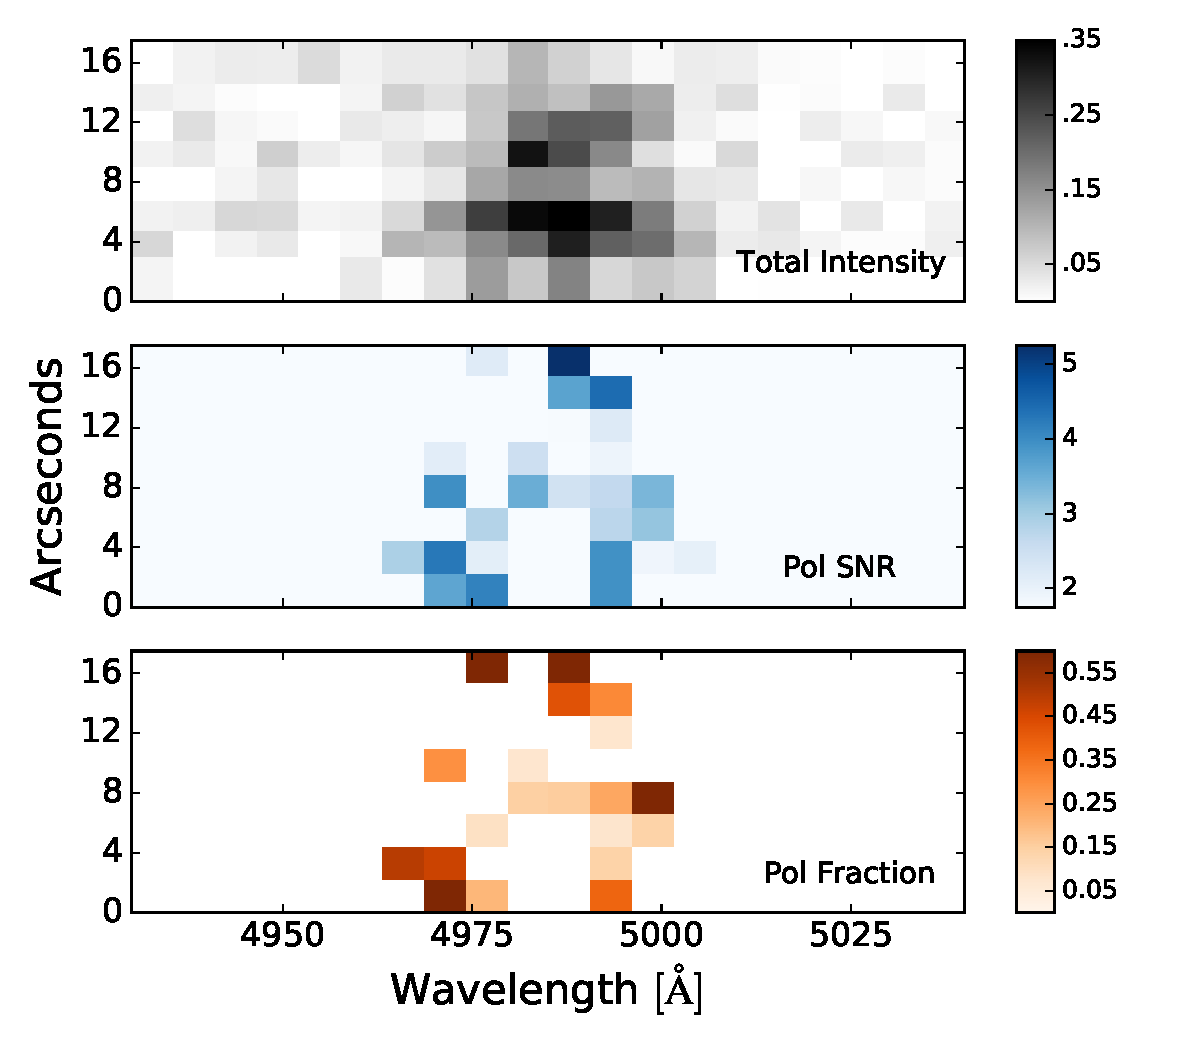
\includegraphics[width=3.65in]{Figures/lyapol/f5_v2.pdf}
\caption[2D total intensity, polarization signal-to-noise, and polarization map]{\textit{Top.}~Total intensity of the 2D \lya~spectrum in bins of 5\AA~by 2-3$''$. \textit{Middle.}~SNR$_p$ map which demonstrates the relative quality of our polarization measurements. SNR$p > 2$ is generally enough for us to discriminate \pol~statistically signicant from zero with 95\% confidence and we show CIs for such bins in \autoref{fig: oned}.  SNR$_p > 3.8$ indicates the Rice distribution is sufficiently Gaussian and we measure polarization with standard errors, also shown in \autoref{fig: oned}. \textit{Bottom.} Map of \pol~determined to be statistically significant from zero with 95\% confidence (lower 95\% confidence bounds greater than zero). For those bins with sufficient SNR$_p$, the bin color reflects the point estimate of \pol, otherwise it  represents the middle value of the CI associated with that bin.}
\label{fig: pol2d}
\end{center}
\end{figure}

In \autoref{fig: pol2d} we present 2D maps of the spectrally binned intensity, SNR$_p$, and polarization of LAB1. In the middle panel we show the SNR$_p$ where we stress that the ``noise" in this equation is not the equivalent of a polarization error. This figure instead serves to give the reader a feeling for the relative quality of our measurements. Comparing the middle and top panels we see that many areas of high intensity have very low polarization signal-to-noise indicating that these regions most likely have very low or no fractional polarization for us to detect with the current data. However, portions of the spectrum exhibiting relatively less intensity have much more significant SNR$_p$. The fraction of polarized light in these bins is relatively more substantial. We also point out that in this SNR$_p$ map we see a range of values from $\sim2$ to $\sim5$ which indicates that for some bins we report point estimates of the fractional polarization while for others we instead provide 95\% CIs. In the bottom panel, we show \pol~in individual bins in which we either have sufficiently high SNR$_p$ or in which we calculate a lower 95\% confidence bound greater than zero.  In general we see higher values of \pol~in the reddest part of the line though we also note some substantial polarization in the blue wing as well. In most cases we see that the central emission region is characterized by low SNR$_p$ and low fractional polarization.

Finally, in \autoref{fig: angles} we present the direction of the polarization vectors, $\chi$, for those spatial elements (\textbf{B-D, F, G}) which have SNR$_p > 2$.   Errors on the polarization angles range from $\sim$6--15\degs.  In this figure we also plot polarization vectors from H11 for comparison, including only those which they measured at or above 2$\sigma$. We see that both sets are generally consistent. Like H11, our angles lie tangentially around the peak of \lya~SB. 

% POLARIZATION ANGLES - POL VECTORS
\begin{figure}[t]
\begin{center}
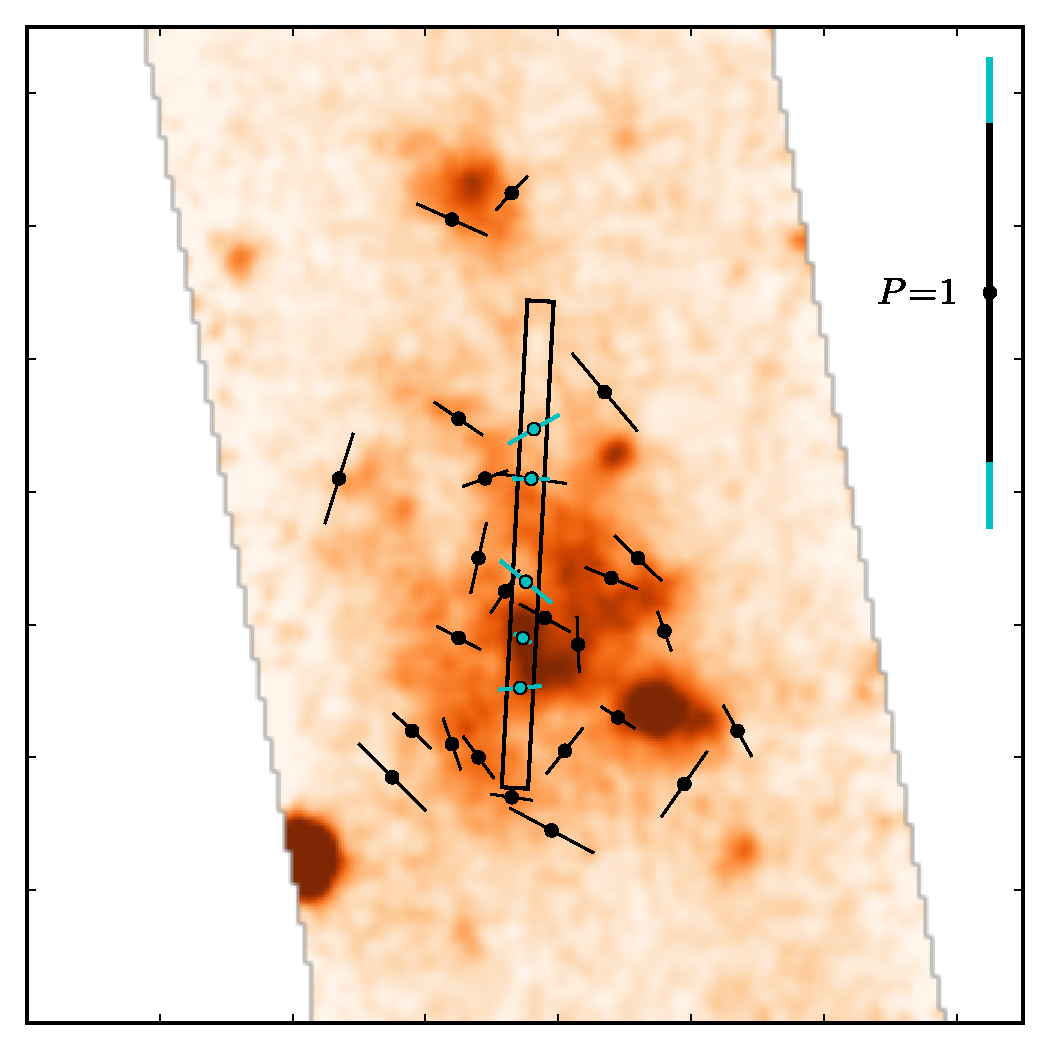
\includegraphics[width=3.25in]{Figures/lyapol/f6_v2.pdf}
\caption[Direction of polarization vectors]{Direction of \lya~polarization vectors. Smoothed total \lya~intensity from H11 overlaid with polarization vectors from H11 (black) and from this analysis (cyan) for those spatial bins from \autoref{fig: totpol}~which have SNR$_p > 2$. Because we measure small polarization amplitude in our bins we use a larger scaling for our vectors in order for the reader to more easily compare the angles we measure with with those presented in H11. Both sets of angles generally lie tangentially about the region of highest \lya~SB.}
\label{fig: angles}
\end{center}
\end{figure}

%%%%%%%%%%%%%%%%%%%%%%%%%%%%%%%%%%%%%%%%%%%%%%%%%%%%%%%
% 	DISCUSSION
%%%%%%%%%%%%%%%%%%%%%%%%%%%%%%%%%%%%%%%%%%%%%%%%%%%%%%%
\section{Discussion and Conclusions}\label{sec: interp}

We have presented deep spectro-polarimetry of  the LAB1 \lya~emission nebula. The data allow us to probe the kinematics and distribution of the neutral gas and reinforce the idea that LAB1 is likely composed of several smaller, more complex regions instead of one large, kinematic structure. In particular, our observations suggest at least a weak outflow in the southern portion of the LAB as we discuss below.

Simulations predict that polarization due to scattering should exhibit a radial dependence on the sky. The region of highest \lya~SB would not be strongly polarized but the polarization would rise with increasing radius \citep{DijkstraLoeb2008}.  The observed polarization of \lya~in the southern portion of the slit is consistent with \lya~photons produced by a luminous galaxy (or galaxies) and scattered at large radii by the surrounding neutral hydrogen. As in H11, we see this signature here, most notably in spatial elements \textbf{B-D} where the peak of the \lya~SB has little observable polarization as shown in spatial element \textbf{C}. North of this location  (\textbf{D}),  we find \pol~= $13.6\pm2.7\%$ which is also consistent with the Voronoi bins from H11 lying on either side of our slit at approximately the same radial distance (see the right side of \autoref{fig: slit}).  Similarly to the south (\textbf{B}), we find total \pol~= $8.59\pm1.9\%$.  Thus we have increasing polarization away from the peak \lya~emission with a radius of $\sim15$ kpc. However, this general trend cannot determine between inflowing or outflowing gas as both are predicted to have this observational signature.

\cite{DijkstraLoeb2008} also predict that, for an envelope of expanding gas, those photons in the bulk of the line profile should exhibit increasing polarization redward of the line core. The strength of this increase depends strongly on the distance from the center of \lya~SB as well as the column density and outflow velocity. In other words, for a given column density and outflow speed, polarization will increase weakly (up to $\sim10\%$) in the reddest part of the wing at the peak of \lya~SB, but will increase substantially (up to $\sim70\%$) at larger radii from this region.  We caution that direct comparison of our data with these simulations comes with a caveat since  we are not integrating over the entire shell with our long-slit observations. Nevertheless, the spectrally resolved polarization in bins \textbf{C} and \textbf{B} at least suggest this behavior.

To see this trend, we first estimate the systemic velocity of the region as the average from four galaxies measured in \oiii~and known to be components of LAB1 \citep{Kubo2015, McLinden2013} (see \autoref{fig: oned}).  We note that these measurements are all within $\sim230$ km/s. Given the width of the \lya~profile, this uncertainty has minimal impact. In this context we can see that the polarization in \textbf{C} is well constrained in the red wing to be at most $\sim20\%$ polarized. Though we are unable to tightly constrain the red wing in bin \textbf{B}, large polarization values are suggested by the detection at 4995\AA, and are not ruled out at longer wavelengths.  This particular polarization pattern can be explained easily with a weak outflowing shell model whereby \lya~photons emitted from an embedded source interact with the expanding shell. Those photons which interact with the receding portion of the shell (from our point of view) are Doppler shifted into the red wing of the profile. Being in the wing of the line profile, these photons see a lower optical depth and thus preferentially escape the medium having only scattered a few times which preserves their polarization. Photons which remain in the core of the profile in the frame of the gas scatter many more times, effectively erasing any polarization signal.

The polarization data presented here provide a framework for future observations of the southern portion of LAB1. The imaging polarimetry of H11 coupled with a recent strong submillimeter source within 1.5$''$ of the peak \lya~intensity \citep{Geach2014} provide the `smoking gun' that there is indeed at least one powerful source embedded in this region, the photons from which are likely scattering at large radii. If there are indeed multiple  sources within about 30 kpc of this region, observations must also provide a mechanism by which these sources can reproduce the spectral polarization signature presented here, namely, a configuration which is consistant with low polarization in the core of the \lya~profile and high polarization in the wings.

However, the picture remains obscure for \textbf{R1} corresponding to our spatial elements \textbf{E-F}. Were \textbf{R1} to be part of the same smooth, kinematic structure as \textbf{R3} we would expect its total \lya~polarization to increase relative to \textbf{R3} due to its increased radius from the galactic center. Instead, we see the total polarization drop and flatten across \textbf{R1}. It's possible that the gas in this region is clumpier or denser than the southern portion of the blob. An increase in the column density of the gas will decrease the observed polarization fraction as additional scatterings tend to isotropize the photons. Another possibility is that this region is powered by flourescence from ionizing radation eminating from the central source. This would naturally explain the lower polarization as this type of \textit{in situ} production of photons is not expected to be highly polarized.   \cite{Weijmans2010} present compelling evidence that suggests this region is kinematically distinct from the rest of LAB1 and thus a third possibility is that this region is instead powered by radiative cooling. Most likely is the possibility that this region is dominated by an embedded souce of its own. Though interesting to speculate, the wavelength dependence of the polarization in these spatial bins is not sufficient for us to further probe the kinematics and polarization properties. 


%%%%%%%%%%%%%%%%%%%%%%%%%%%%%%%%%%%%%%%%%%%%%%%%%%%%%%%
% 	Polarization in the Future
%%%%%%%%%%%%%%%%%%%%%%%%%%%%%%%%%%%%%%%%%%%%%%%%%%%%%%%

\section{The Future of \lya~Polarization}\label{sec: future}
With another successful detection of the spectral dependence of \lya~polarization the question arises: What does the future hold for \lya~polarization? Additionally, should emphasis be placed on imaging or spectral polarimetry? The integration times for either mode are similar in magnitude and require a substantial commitment so the choice between methods is not a trivial one.  

We have explicitly demonstrated that much information can be gleaned from the spectral dependence of the polarization signal. In particular, features emerge which narrowband imaging polarimetry simply cannot detect. Not only are we able to detect the wavelength dependence for many of our spatial bins but we also find high polarization upwards of 60\% in portions of the \lya~profiles -- information which is completely lost in imaging polarimetry. While imaging polarimetry can confirm the presence of scattering and probe the overall geometry of the scattering medium, it cannot probe the kinematics of the system to determine potential outflows or inflows. Furthermore, the spectrally integrated polarization can still provide spatial clues as to any existing radial dependence with advantageous slit placement. Because the geometry of the blob is important to the overall detection of a polarization signal, spectropolarimetry should not be conducted blindly but instead by guided by spatial information obtained from the already existing narrowband surveys of LABs as well as IFUs. 

Though it remains to be seen, suggestions have arisen that the next generation of $\sim$30 m telescopes could extend \lya~polarization studies. This is supported in that all projected Extremely Large Telescopes (ELT) have proposed polarimetry as a necessary part of their instrument suite.  On the E-ELT, the \textit{Exo-Planet Imaging Camera and Spectrograph} \citep[\textit{EPICS},][]{Kasper2008} includes the \textit{EPOL} polarimeter \citep{Keller2010}.  The Thirty Meter Telescope has discussed plans to include the \textit{Second-Earth Imager for TMT} \citep{SEIT}. And the Giant Magellan Telescope has discussed spectro-polarimetric capabilities as necessary to meeting their science goals \citep{GMTscience}.  Off the ground, several probe-scale NASA space missions have been proposed to study exoplanetary systems such as the AFTA and ``EXO" missions \citep{Stapelfeldt2014, Seager2014}, with considerable emphasis given to polarimeters to enrich the science output. While many of these projects focus on imaging polarimetry, the UVMag consortium has proposed the Arago space mission which would be devoted to unprecedented spectropolarimetry from the FUV through the NIR \citep{Pertenais2014}.  This field is currently driven almost exclusively by exo-planetary science for studying the scattering off planetary atmospheres and circumstellar disks but it is the development of such instrumentation which is of greatest importance. At this stage, we cannot say whether we will be able to point one of these instruments directly towards a \lya~blob without slight modification of the initial design or incorporation of additional settings but it is optically plausible \citep{Hayes2011}.

In the meantime, much can still be accomplished from the ground with 8 m class telescopes. To date, only three \lya~emitting sources have been studied in depth: LAB1 \citep[][and this work]{HayesScarlata2011}, LABd05 \citep{Prescott2011} and radio galaxy TXS 0211--122, known to be associated with a 100 kpc scale \lya~nebula \citep{Humphrey2013}. Radio-quiet LABs were first targeted due to their apparently controversial nature unlike high redshift radio galaxies (HzRGs) which did not pose an energy problem.  With the discovery that a HzRG is at least partially polarized due to \lya~scattering, it behooves us to test further what relationship, if any, exists between radio-loud and -quiet nebulae. Compact \lya~sources also remain unexplored with the polarimeter. Though targeting resolved objects ensures that the Stokes parameters do not all cancel, symmetry is likely broken in most systems. Thus we may expect a measureable signal from LAEs \citep{LeeAhn1998}.
 
Additionally, the interpretation of \lya~polarization is still a challenging prospect of its own. Most state-of-the-art simulations assume density and kinematic structures that are still unrealistic in that variations proceed smoothly. What is urgently needed is the implementation of \lya~polarization in all \lya~radiative transport codes to generate predictions for various applications including clumpy and filimentary media as well as non-spherically symmetric geometries. While some work has already been done in this area \citep{DijkstraKramer2012}, there is still much to be explored in terms of predicting observable polarized \lya~line profiles. With the current limitation on instumentation coupled with exacting observations, we need dedicated theoretical and observational developments that proceed in tandem. 
\newline

We thank the anonymous referee for the useful comments that significantly improved the analysis and presentation of our results. Additionally, MB and CS are grateful to J\'{e}r\'{e}my Blaizot and Maxime Trebitsch for proofing the manuscript and providing feedback which helped to clarify the text. 

\end{document}
